%%Correcciones menores Gabriel:

%Figura 3.12 ---->> Sacar H2O adsorbida cambiar x Vapor de H2O
%Figura 4.1  ---->> Confusa..... destacar mejor con alguna figura inset u otra cosa
%Figura 3.12 ---->> Cambiar pulverizado x denso (óxido de silicio denso)
%Citar lo de la doble distribuciones con figura incluida


%%%%%%%%%%%%%%%%%%%%%%%%%%%%%%%%%%%%%%%%%%%%%%%%%
% 											                       	%
%   TESIS PARA DOCTORADO DE GUSTAVO GIMENEZ     %
%                                               %
%%%%%%%%%%%%%%%%%%%%%%%%%%%%%%%%%%%%%%%%%%%%%%%%%

%Compila Versión Final
\documentclass[a4paper,10pt,twoside,openright,titlepage]{book}

%Compila como borrador
%\documentclass[draft,a4paper,10pt,twoside,openright,titlepage]{book}

%Muestra marco para ver encabezados, cuerpo del texto, etc.
%\usepackage{showframe}

%Configuraciones
%----------------------------------------------------------------------------------------------
  %Acá van los paquetes y las definiciones de colores, renombrar comandos, nuevo comandos, etc.
  %Sección de Plugins
%--------------------------------------------------------------------------
   %Idioma, fuentes y entrada de teclado
   \usepackage[spanish,activeacute,es-tabla,es-lcroman]{babel}
   \usepackage[utf8]{inputenc}
   \usepackage{lmodern}

   %Suprime el Warning de multiples PDF por pagina
   \pdfsuppresswarningpagegroup=1
   
   %Paquete para adaptar la Bibliografia al Español
   \usepackage[datename]{babelbib}

   %Para manejar la forma en que se presentan las citas
   \usepackage[superscript]{cite}
       
   % Paquete para gestionar imágenes jpg
   \usepackage{graphicx}

   % Paquete para hacer cuadros
   \usepackage{boxedminipage} 

   %Paquete para colocar imagenes en el medio del texto
   \usepackage{wrapfig}

   %paquete para lenguaje matematico y símbolos
   \usepackage{amsmath,amssymb,amsfonts,latexsym,cancel,esint}

   % Paquete para poner colores
   \usepackage[usenames,dvipsnames]{color}

   %Para la justificación, formato y texto de los caption de las figuritas y tablas
   \usepackage{caption}

   %Paquete para poder poner imagenes una al lado de la otra
   \usepackage{subcaption}
   
   %Para hacer graficos cons tikz, con gnuplot y poder exportarlos como pdf
       \usepackage{tikz}
       \usepackage{tikzpagenodes}
     
           %Librerias Tikz Extra
             \usetikzlibrary{shapes,arrows}
             \usetikzlibrary{shapes.arrows, fadings}
             \usetikzlibrary{shadows.blur}
             \usetikzlibrary{shapes.symbols}
             \usetikzlibrary{decorations.pathreplacing}
             \usetikzlibrary{fit}
             \usetikzlibrary{calc}
             \usetikzlibrary{positioning}
             \usetikzlibrary{matrix}

   %Para hacer lineas gruesa y tablas lindas
   \usepackage{booktabs}

   %Para Formatear los capitulos
   \usepackage{titlesec}

   %Herramientas para parches
   %Yo lo use para Cambiar el nombre de la Bibliografia
   \usepackage{etoolbox}
   
   %Para Tablas multicolumnas, multifilas
   \usepackage{multirow,multicol,array} 

   %Para rota Texto
   \usepackage{rotating} 

   %Para los Indices parciales en las portadas de los capitulos
   \usepackage[nohints]{minitoc}

   %Paquete para personalizar encabezados y notas al pie
   \usepackage{fancyhdr}   

   %Para que no numere las paginas en blanco (borrar los header y footnotes)
   \usepackage{emptypage}

   %Para carga Atributos, Propiedades y Titulos al PDF
   \usepackage[hidelinks,colorlinks]{hyperref}

   %Para la lista de abreviaturas
   \usepackage[acronym,nonumberlist,nomain]{glossaries}
   \makeglossaries
   
   %Para hacer un indice alfabetico
   \usepackage{imakeidx}
   \makeindex[columns=2, options= -s Tesis.ist]
   \indexsetup{othercode=\footnotesize}
   %Muestra el indexado en el costado
   %\usepackage{showidx}
   
   %Para Imprimir el LayOut del documento
   \usepackage{layout}

   %Para hacer quimica
   \usepackage{chemfig}

   %para meter text de relleno
   \usepackage{blindtext}

   %Paquete gestor de unidades
   \usepackage[version-1-compatibility]{siunitx}
   \sisetup{output-decimal-marker = {,}}

   %Para Colocar objetos en el fondo, en mi caso los indicadores laterales
   \usepackage[contents={},opacity=1,scale=1,color=black]{background}
   %--------------------------------------------------------------------------

%SUprimir log de Overfull y UNdelfull
%--------------------------------------------------------------------------
    \newcommand{\NoBadBoxesLog}{
      \hfuzz=\maxdimen \vfuzz=\maxdimen 
      \newdimen\hfuzz  \let\vfuzz=\hfuzz
      \hbadness=10000    \vbadness=10000 
      \newcount\hbadness \let\vbadness=\hbadness 
      }

%Propiedades del Documento
%--------------------------------------------------------------------------
   \hypersetup{
   pdftitle={Tesis Gustavo Giménez},
   pdfauthor={Gustavo Giménez},
   pdfsubject={Tesis Doctoral}, %subject of the document
   pdfcreator={Tex},
   pdfproducer={PDFLatex},
   pdfkeywords={UBA,nanomateriales,MEMS,NEMS,INTI},
   % %pdftoolbar=false, % toolbar hidden
   pdfmenubar=true, %menubar shown
   pdfhighlight=/O, %effect of clicking on a link
   % pdfpagemode=UseOutlines,%UseNone, %aucun mode de page
   % pdfpagelayout=TwoPageRight,%SinglePage, %ouverture en simple page
   % pdffitwindow=true, %pages ouvertes entierement dans toute la fenetre
   % bookmarksopenlevel=2,
   %    colorlinks=false,       % false: boxed links; true: colored links
   linkcolor=black,          % color of internal links (change box color with linkbordercolor)
   citecolor=grisoscuro,        % color of links to bibliography
   urlcolor=grisoscuro,          % color of external link
   %backref=true
   }
   %--------------------------------------------------------------------------

  %Aca Pongo los archivos de Formato Personalizados:
  %Margenes, tamaños, titulos, lineas, capitulos, caption, etc.
  %%%%%%%%%%%%%%%%%%%%%%%%%%%%%%%%%%%%%%%%%%%%%%%%%%%%%%%%%%%%%%%%%%%
%   Aca van los Formatos Personalizados de todo el documento	  %
%%%%%%%%%%%%%%%%%%%%%%%%%%%%%%%%%%%%%%%%%%%%%%%%%%%%%%%%%%%%%%%%%%%

%Formato General del Documento
%------------------------------------------------------------
 
 %Intercambio los margenes derechos e izquierdos
 %------------------------------------------------------------
 \let\tmp\oddsidemargin
 \let\oddsidemargin\evensidemargin
 \let\evensidemargin\tmp
 \reversemarginpar

 %La class book por default pone un espacio para notas marginales en el lado derecho para las paginas 
 %impares y en el izquierdo para las pares, yo lo invertí para que me quede mas amplio el espacio para 
 %la unión de las paginas en el lomo del libro, la costura.
 

    % Defino los margenes bien personalizados.
    % Zona de la pagina ocupada por el texto
    % Información detallada: http://en.wikibooks.org/wiki/LaTeX/Page_Layout
    % O descomentar la linea  \layout 
	% \layout
 	%------------------------------------------------------------------------------------------------------------------ 
 		% 	    \hoffset = 2 cm                          % OffSet desde el borde izquierdo de la pagina
 		% 		\voffset = 2 cm                          % OffSet desde el borde Superior de la pagina
 		% 		\topmargin = -2.54 cm                    % Desde el borde superior de la pagina hasta el texto + 1 inch
		% 		\oddsidemargin = -2.54 cm                % Desde el borde izquierdo de la pagina hasta el texto + 1 inc
		% 		\headsep =  0 cm                         % Separación entre el encabezado y el texto	
 		% 		\textwidth = 17 cm                       % Ancho del texto y define margen derecho - margen - offset
 		% 		\textheight = 23.5 cm                    % Largo del texto y margen inferior - margen - offset
 		% 		\headheight = 0.1 cm                     % Espacio del cuadro de texto del Encabezado
		% 		\footskip = 1.5 cm                       %Espacio para el pie de pagina 
 		%    	\marginparwidth = 95pt					 %Ancho de las notas al margen
 		% 	    \marginparsep = 25pt					 %Separación margen-texto
 	%------------------------------------------------------------------------------------------------------------------

%Formato de las Cabeceras, los Pie de Pagina y la numeracion
%------------------------------------------------------------
	%Cambio el Header para que no salga la palabra "Capitulo"
	\addto{\captionsspanish}{\def\chaptername{}}

	%Cambio el Color de la Headrule
	\let\headruleORIG\headrule
	\renewcommand{\headrule}{\color{grisoscuro}\headruleORIG}
	
	%Estilo de las Cabeceras y Pie de pagina para los precapitulos
	\fancypagestyle{frontmatter}{
		\fancyhead{}   							%Borro Cabeceras
		\renewcommand{\headrulewidth}{0pt} 		%Borro Headrule							
		\fancyfoot[C]{\thepage}    				%Numero de pagina centrado
		}
	
	%Estilo de las Cabeceras y Pie de pagina para el cuerpo principal
	\fancypagestyle{mainmatter}{
		\fancyfoot{}													   % Borro las paginas al pie
		\renewcommand{\headrulewidth}{1pt}  							   % Borro la Linea del encabecera		
		\fancyfoot[LE,RO]{\color{grisoscuro}\bfseries\thepage}             % Pongo el numero de pagina en todas la paginas en el lado exterior
	 	\fancyhead[LE]{\color{grisoscuro}\bfseries\nouppercase{\leftmark}} % Pongo el capitulo arriba a la derecha en las paginas pares 
	    \fancyhead[RO]{\color{grisoscuro}\bfseries\nouppercase{\rightmark}}% Pongo la sección arriba a la izquierda en las impares
	    }
	
	%Estilo de las Cabeceras y Pie de pagina para los postcapitulos
	\fancypagestyle{backmatter}{
		\fancyhead{}
		\fancyfoot{}										    %Borro Cabeceras
		\renewcommand{\headrulewidth}{0pt} 				        %Borro Headrule							
		\fancyfoot[LE,RO]{\color{grisoscuro}\bfseries\thepage}  % Pongo el numero de pagina en todas la paginas en el lado exterior
		}
 %--------------------------------------------------------------

%Formato de las Etiquetas (Referencias, Capitulos, etc)
%------------------------------------------------------------
 %Cambiar el nombre de Bibliografia por Referencias
 \patchcmd{\thebibliography}{\chapter*{\bibname}}{\chapter*{Referencias}}{}{}
 %-------------------------------------------------------------

%Formato de los Titulos de los capitulos
%------------------------------------------------------------
    %Ubicación Espacial del conjunto "Titulo" de Capitulos
      \titlespacing*{\chapter}  %Seccion a modificar
 			 {-3cm}             %Indentación Izquierda
 			 {-1cm}            %Espacio Anterior
 			 {50pt} 	        %Espacio Posterior
 			 [0cm]	           %Indentación Derecha
    
    %Formato para Todos los Capitulos, solo lo uso para el Indice General
	 \titleformat{\chapter}[display]
			{\Huge\filleft\scshape\color{grisoscuro}}      	 %Formato para etiqueta y texto
	 		{}	
	 		{20pt}  	     %Separación Etiqueta/Texto                
	 		{}               %Codigo anterior
	 		[]   %Codigo Posteior  \titlerule\vspace{2ex}\filright\vspace{2ex}]
	
	%Variables para ubicar el numero de capitulo	
	 \newlength\NumCapX
	 \setlength\NumCapX{-1cm}  %Aumentar es mas para arriba
	 \newlength\NumCapY	
	 \setlength\NumCapY{-2cm}  %Aumentar es mas para el exterior		

	%Formato para el titulo de los Indices
	 \newcommand{\FormatoIndice}{
	 		\titleformat{name=\chapter,numberless}[display]						 %Sin Numerar
			{\Huge\filleft\scshape\color{grisoscuro}}      	 %Formato para etiqueta y texto
	 		{\begin{tikzpicture}[remember picture,overlay] 						 %Cuadrado con el numero
				\node[at={($(\NumCapX,\NumCapY)$)},anchor=center,font=\rmfamily\fontsize{300pt}{0pt}\bf\selectfont\color{grisoscuro},opacity=0.2] (texto) {\textit{I}};
				\node at (-12.16,-2) {\rule{25cm}{0.5mm}};
				\end{tikzpicture}
			}		
	 		{20pt}  	    				 %Separación Etiqueta/Texto                
	 		{\vspace*{-0.15cm}}              %Codigo anterior
	 		[]   				 %Codigo Posteior
	 } 

	%Formato Para los Capitulos Numerados y que el título ocupa una sola linea
 	 \newcommand{\FormatoCapituloUnaLinea}{
 		\titleformat{\chapter}     						     %Seccion a modificar
			[display]					 			 		 %Formato separado en dos renglones separados
			{\Huge\filleft\scshape\color{grisoscuro}}      	 %Cuadrado con el numero
			{\begin{tikzpicture}[remember picture,overlay]
				\node[at={($(\NumCapX,\NumCapY)$)},anchor=center,font=\rmfamily\fontsize{300pt}{0pt}\bf\selectfont\color{grisoscuro},opacity=0.2] (texto) {\textit{\thechapter}};
				\node at (-12.16,-2) {\rule{25cm}{0.5mm}};
			    \end{tikzpicture}
			}
	 		{20pt}  	     %Separación Etiqueta/Texto                
	 		{}               %Codigo anterior
	 		[]   %Codigo Posteior 
	 		}	
 	 		
	%Formato Para los Capitulos Numerados y que el título ocupa dos lineas
 	 \newcommand{\FormatoCapituloDosLineas}{
 		\titleformat{\chapter}     						     %Seccion a modificar
			[display]					 			 		 %Formato separado en dos renglones separados
			{\Huge\filleft\scshape\color{grisoscuro}}      	 %Cuadrado con el numero
			{\begin{tikzpicture}[remember picture,overlay]
				\node[at={($(\NumCapX,\NumCapY)$)},anchor=center,font=\rmfamily\fontsize{300pt}{0pt}\bf\selectfont\color{grisoscuro},opacity=0.2] (texto) {\textit{\thechapter}};
				\node at (-12.16,-2) {\rule{25cm}{0.5mm}};
				\end{tikzpicture}
			}
	 		{20pt}  	     		 %Separación Etiqueta/Texto                
	 		{\vspace*{-1.05cm}}      %Codigo anterior
	 		[]  		 %Codigo Posteior  
	 		}	
	
	%Formato para el titulo de los Anexos
	 \newcommand{\FormatoAnexoA}{
	 		\titleformat{name=\chapter,numberless}[display]						 %Sin Numerar
			{\Huge\filleft\scshape\color{grisoscuro}}      	 %Formato para etiqueta y texto
	 		{\begin{tikzpicture}[remember picture,overlay] 						 %Cuadrado con el numero
				\node[at={($(\NumCapX,\NumCapY)$)},anchor=center,font=\rmfamily\fontsize{300pt}{0pt}\bf\selectfont\color{grisoscuro},opacity=0.2] (texto) {\textit{A}};
				\node at (-12.16,-2) {\rule{25cm}{0.5mm}};
				\end{tikzpicture}
			}		
	 		{20pt}  	    				 %Separación Etiqueta/Texto                
	 		{\vspace*{-1.05cm}}              %Codigo anterior
	 		[]   				 %Codigo Posteior
	 }
	 \newcommand{\FormatoAnexoB}{
	 		\titleformat{name=\chapter,numberless}[display]						 %Sin Numerar
			{\Huge\filleft\scshape\color{grisoscuro}}      	 %Formato para etiqueta y texto
	 		{\begin{tikzpicture}[remember picture,overlay] 						 %Cuadrado con el numero
				\node[at={($(\NumCapX,\NumCapY)$)},anchor=center,font=\rmfamily\fontsize{300pt}{0pt}\bf\selectfont\color{grisoscuro},opacity=0.2] (texto) {\textit{B}};
				\node at (-12.16,-2) {\rule{25cm}{0.5mm}};
				\end{tikzpicture}
			}		
	 		{20pt}  	    				 %Separación Etiqueta/Texto                
	 		{\vspace*{-0.15cm}}              %Codigo anterior
	 		[]   				 %Codigo Posteior
	 }

	  \newcommand{\FormatoAnexoC}{
	 		\titleformat{name=\chapter,numberless}[display]						 %Sin Numerar
			{\Huge\filleft\scshape\color{grisoscuro}}      	 %Formato para etiqueta y texto
	 		{\begin{tikzpicture}[remember picture,overlay] 						 %Cuadrado con el numero
				\node[at={($(\NumCapX,\NumCapY)$)},anchor=center,font=\rmfamily\fontsize{300pt}{0pt}\bf\selectfont\color{grisoscuro},opacity=0.2] (texto) {\textit{C}};
				\node at (-12.16,-2) {\rule{25cm}{0.5mm}};
				\end{tikzpicture}
			}		
	 		{20pt}  	    				 %Separación Etiqueta/Texto                
	 		{\vspace*{-0.15cm}}              %Codigo anterior
	 		[]   				 %Codigo Posteior
	 }

	%Formato para el titulo del Capitulo Referencias
	  \newcommand{\FormatoReferencias}{
	  		\titleformat{name=\chapter,numberless}[display]  %Sin Numerar
		 	{\Huge\filleft\scshape\color{grisoscuro}}      	 %Formato para etiqueta y texto
	  	 	{\begin{tikzpicture}[remember picture,overlay]   %Cuadrado con el numero
		 		\node[at={($(\NumCapX,\NumCapY)$)},anchor=center,font=\rmfamily\fontsize{300pt}{0pt}\bf\selectfont\color{grisoscuro},opacity=0.2] (texto) {\textit{R}};
		 		\node at (-12.16,-2) {\rule{25cm}{0.5mm}};
		 		\end{tikzpicture}
		 	}
	  		{20pt}  	     %Separación Etiqueta/Texto                
	  		{}               %Codigo anterior
	  		[]   %Codigo Posteior  
	  }

	%-------------------------------------------------------------

%Indicador lateral de capitulos
%------------------------------------------------------------
	
	%Definiciones Generales de variables para los loops if
	 \newif\ifMaterialInd
	 \newif\ifMaterialCap
	 \newif\ifMaterialAxUno
	 \newif\ifMaterialAxDos
	 \newif\ifMaterialAxTres
	 \newif\ifMaterialBib
	 \newif\ifMaterialAlf

	%Posiciones Iniciales de los indicadores laterales
	 \newlength\PosVertical
	 \setlength\PosVertical{6.56cm}       %Aumentar es mas para arriba
	 \newlength\PosHorizontal	
	 \setlength\PosHorizontal{10.2cm}  %Aumentar es mas para el exterior

	%Con \AddLabelsInd se agregan los indicadores laterales de los indices
	 \newcommand\AddLabelsInd{
	 \MaterialIndtrue
	 \AddEverypageHook{
	 	\ifMaterialInd
	 		\ifodd\value{page} 
  				\backgroundsetup{
	 				  angle=90, %Ojo!! Invierte las coordenadas!!
	 				  contents={
	 				  \begin{tikzpicture}[remember picture,overlay] 
	 				    \node[at={($(\PosVertical,-\PosHorizontal)$)}] % Las coordenadas son (y,-x)
	 					(cuadrado) {\tikz {\draw[draw=none,fill=grisoscuro] (0,0) rectangle ++(3,1);} };
	 					\node[at={($(cuadrado.center)+(0,0.2)$)},anchor=center,font=\large\filleft\scshape,text=white](texto) {Índice};
	 					\end{tikzpicture}
	 				  }
	 				 }
  			\else
	 				 \backgroundsetup{
	 				  angle=90, %Ojo!! Invierte las coordenadas!!
	 				  contents={
	 				    \begin{tikzpicture}[remember picture,overlay] 
	 				    \node[at={($(\PosVertical,\PosHorizontal)$)}] % Las coordenadas son (y,-x)
	 					(cuadrado) {\tikz {\draw[draw=none,fill=grisoscuro] (0,0) rectangle ++(3,1);} };
	 					\node[at={($(cuadrado.center)+(0,-0.1)$)},anchor=center,font=\large\filleft\scshape,text=white](texto) {Índice};
	 					\end{tikzpicture}
	 				  }
	 				 }
  			\fi
	 	\BgMaterial
	 	\else\relax\fi}
	 	}	 

	%Con \AddLabelsCap se agregan los indicadores laterales de los capitulos
	 \newcommand\AddLabelsCap{
	 \MaterialCaptrue
	 \AddEverypageHook{
	 	\ifMaterialCap
	 		\ifodd\value{page} 
  				\backgroundsetup{
	 				  angle=90, %Ojo!! Invierte las coordenadas!!
	 				  contents={
	 				  \begin{tikzpicture}[remember picture,overlay] 
	 				    \node[at={($(\PosVertical,-\PosHorizontal)-(\thechapter,0)$)}] % Las coordenadas son (y,-x)
	 					(cuadrado) {\tikz {\draw[draw=none,fill=grisoscuro] (0,0) rectangle ++(3,1);} };
	 					\node[at={($(cuadrado.center)+(0,0.2)$)},anchor=center,font=\large\filleft\scshape,text=white](texto) {Capítulo \thechapter};
	 					\end{tikzpicture}
	 				  }
	 				 }
  			\else
	 				 \backgroundsetup{
	 				  angle=90, %Ojo!! Invierte las coordenadas!!
	 				  contents={
	 				    \begin{tikzpicture}[remember picture,overlay] 
	 				    \node[at={{($(\PosVertical,\PosHorizontal)-(\thechapter,0)$)}}] % Las coordenadas son (y,-x)
	 					(cuadrado) {\tikz {\draw[draw=none,fill=grisoscuro] (0,0) rectangle ++(3,1);} };
	 					\node[at={($(cuadrado.center)+(0,-0.1)$)},anchor=center,font=\large\filleft\scshape,text=white](texto) {Capítulo \thechapter};
	 					\end{tikzpicture}
	 				  }
	 				 }
  			\fi
	 	\BgMaterial
	 	\else\relax\fi}
	 	}

	%Con \AddLabelsAxUno se agregan los indicaroes laterales Anexo A
     \newcommand\AddLabelsAxUno{
	 \MaterialAxUnotrue
	 \AddEverypageHook{
	 	\ifMaterialAxUno
	 		\ifodd\value{page}
  				\backgroundsetup{
	 				  angle=90, %Ojo!! Invierte las coordenadas!!
	 				  contents={
	 				  \begin{tikzpicture}[remember picture,overlay] 
	 					\node[at={($(\PosVertical,-\PosHorizontal)-(\thechapter+1,0)$)}] % Las coordenadas son (y,-x)
	 					(cuadrado) {\tikz {\draw[draw=none,fill=grisoscuro] (0,0) rectangle ++(3,1);} };
	 					\node[at={($(cuadrado.center)+(0,0.2)$)},anchor=center,font=\large\filleft\scshape,text=white](texto) {Anexo A};
	 					\end{tikzpicture}
	 				  }
	 				 }
  			\else
	 				 \backgroundsetup{
	 				  angle=90, %Ojo!! Invierte las coordenadas!!
	 				  contents={
	 				    \begin{tikzpicture}[remember picture,overlay] 
	 				    \node[at={($(\PosVertical,\PosHorizontal)-(\thechapter+1,0)$)}]  % Las coordenadas son (y,-x)
	 				    (cuadrado) {\tikz {\draw[draw=none,fill=grisoscuro] (0,0) rectangle ++(3,1);} };
	 				    \node[at={($(cuadrado.center)+(0,-0.1)$)},anchor=center,font=\large\filleft\scshape,text=white] (texto) {Anexo A};
	 					\end{tikzpicture}
	 				  }
	 				 }
  			\fi
	 	\BgMaterial
	 	\else\relax\fi}
	 	}

	%Con \AddLabelsAxDos se agregan los indicaroes laterales Anexo B
	 \newcommand\AddLabelsAxDos{
	 \MaterialAxDostrue
	 \AddEverypageHook{
	 	\ifMaterialAxDos
	 		\ifodd\value{page}
  				\backgroundsetup{
	 				  angle=90, %Ojo!! Invierte las coordenadas!!
	 				  contents={
	 				  \begin{tikzpicture}[remember picture,overlay] 
	 					\node[at={($(\PosVertical,-\PosHorizontal)-(\thechapter+2,0)$)}] % Las coordenadas son (y,-x)
	 					(cuadrado) {\tikz {\draw[draw=none,fill=grisoscuro] (0,0) rectangle ++(3,1);} };
	 					\node[at={($(cuadrado.center)+(0,0.2)$)},anchor=center,font=\large\filleft\scshape,text=white](texto) {Anexo B};
	 					\end{tikzpicture}
	 				  }
	 				 }
  			\else
	 				 \backgroundsetup{
	 				  angle=90, %Ojo!! Invierte las coordenadas!!
	 				  contents={
	 				    \begin{tikzpicture}[remember picture,overlay] 
	 				    \node[at={($(\PosVertical,\PosHorizontal)-(\thechapter+2,0)$)}]  % Las coordenadas son (y,-x)
	 				    (cuadrado) {\tikz {\draw[draw=none,fill=grisoscuro] (0,0) rectangle ++(3,1);} };
	 				    \node[at={($(cuadrado.center)+(0,-0.1)$)},anchor=center,font=\large\filleft\scshape,text=white] (texto) {Anexo B};
	 					\end{tikzpicture}
	 				  }
	 				 }
  			\fi
	 	\BgMaterial
	 	\else\relax\fi}
	 	}
	
	%Con \AddLabelsAxDos se agregan los indicaroes laterales Anexo C
	 \newcommand\AddLabelsAxTres{
	 \MaterialAxTrestrue
	 \AddEverypageHook{
	 	\ifMaterialAxTres
	 		\ifodd\value{page}
  				\backgroundsetup{
	 				  angle=90, %Ojo!! Invierte las coordenadas!!
	 				  contents={
	 				  \begin{tikzpicture}[remember picture,overlay] 
	 					\node[at={($(\PosVertical,-\PosHorizontal)-(\thechapter+3,0)$)}] % Las coordenadas son (y,-x)
	 					(cuadrado) {\tikz {\draw[draw=none,fill=grisoscuro] (0,0) rectangle ++(3,1);} };
	 					\node[at={($(cuadrado.center)+(0,0.2)$)},anchor=center,font=\large\filleft\scshape,text=white](texto) {Anexo C};
	 					\end{tikzpicture}
	 				  }
	 				 }
  			\else
	 				 \backgroundsetup{
	 				  angle=90, %Ojo!! Invierte las coordenadas!!
	 				  contents={
	 				    \begin{tikzpicture}[remember picture,overlay] 
	 				    \node[at={($(\PosVertical,\PosHorizontal)-(\thechapter+3,0)$)}]  % Las coordenadas son (y,-x)
	 				    (cuadrado) {\tikz {\draw[draw=none,fill=grisoscuro] (0,0) rectangle ++(3,1);} };
	 				    \node[at={($(cuadrado.center)+(0,-0.1)$)},anchor=center,font=\large\filleft\scshape,text=white] (texto) {Anexo C};
	 					\end{tikzpicture}
	 				  }
	 				 }
  			\fi
	 	\BgMaterial
	 	\else\relax\fi}
	 	}
	 	
	%Con \AddLabelsBib se agregan los indicaroes laterales para la bibliografia
	 \newcommand\AddLabelsBib{
	 \MaterialBibtrue
	 \AddEverypageHook{
	 	\ifMaterialBib
	 		\ifodd\value{page}
  				\backgroundsetup{
	 				  angle=90, %Ojo!! Invierte las coordenadas!!
	 				  contents={
	 				  \begin{tikzpicture}[remember picture,overlay] 
	 					\node[at={($(\PosVertical,-\PosHorizontal)-(\thechapter+4,0)$)}] % Las coordenadas son (y,-x)
	 					(cuadrado) {\tikz {\draw[draw=none,fill=grisoscuro] (0,0) rectangle ++(3,1);} };
	 					\node[at={($(cuadrado.center)+(0,0.2)$)},anchor=center,font=\large\filleft\scshape,text=white](texto) {Referencias};
	 					\end{tikzpicture}
	 				  }
	 				 }
  			\else
	 				 \backgroundsetup{
	 				  angle=90, %Ojo!! Invierte las coordenadas!!
	 				  contents={
	 				    \begin{tikzpicture}[remember picture,overlay] 
	 				    \node[at={($(\PosVertical,\PosHorizontal)-(\thechapter+4,0)$)}]  % Las coordenadas son (y,-x)
	 				    (cuadrado) {\tikz {\draw[draw=none,fill=grisoscuro] (0,0) rectangle ++(3,1);} };
	 				    \node[at={($(cuadrado.center)+(0,-0.1)$)},anchor=center,font=\large\filleft\scshape,text=white] (texto) {Referencias};
	 					\end{tikzpicture}
	 				  }
	 				 }
  			\fi
	 	\BgMaterial
	 	\else\relax\fi}
	 	}

	%Con \AddLabelsAlf se agregan los indicadores laterales del indice alfabetico
	 \newcommand\AddLabelsAlf{
	 \MaterialAlftrue
	 \AddEverypageHook{
	 	\ifMaterialAlf
	 		\ifodd\value{page} 
  				\backgroundsetup{
	 				  angle=90, %Ojo!! Invierte las coordenadas!!
	 				  contents={
	 				  \begin{tikzpicture}[remember picture,overlay] 
	 				    \node[at={($(\PosVertical,-\PosHorizontal)-(\thechapter+6,0)$)}] % Las coordenadas son (y,-x)
	 					(cuadrado) {\tikz {\draw[draw=none,fill=grisoscuro] (0,0) rectangle ++(4,1);} };
	 					\node[at={($(cuadrado.center)+(0,0.2)$)},anchor=center,font=\large\filleft\scshape,text=white](texto) {Índice Alfabético};
	 					\end{tikzpicture}
	 				  }
	 				 }
  			\else
	 				 \backgroundsetup{
	 				  angle=90, %Ojo!! Invierte las coordenadas!!
	 				  contents={
	 				    \begin{tikzpicture}[remember picture,overlay] 
	 				    \node[at={($(\PosVertical,\PosHorizontal)-(\thechapter+6,0)$)}] % Las coordenadas son (y,-x)
	 					(cuadrado) {\tikz {\draw[draw=none,fill=grisoscuro] (0,0) rectangle ++(4,1);} };
	 					\node[at={($(cuadrado.center)+(0,-0.1)$)},anchor=center,font=\large\filleft\scshape,text=white](texto) {Índice Alfabético};
	 					\end{tikzpicture}
	 				  }
	 				 }
  			\fi
	 	\BgMaterial
	 	\else\relax\fi}
	 	}	 	
	
	%Con estos comandos se borran los indicadores laterales	
	 \newcommand\RemoveLabelsInd{\MaterialIndfalse}
	 \newcommand\RemoveLabelsCap{\MaterialCapfalse}
	 \newcommand\RemoveLabelsAxUno{\MaterialAxUnofalse}
	 \newcommand\RemoveLabelsAxDos{\MaterialAxDosfalse}
	 \newcommand\RemoveLabelsAxTres{\MaterialAxTresfalse}
	 \newcommand\RemoveLabelsBib{\MaterialBibfalse}
	 \newcommand\RemoveLabelsAlf{\MaterialAlffalse}

%Formato de los mini-indices de los capitulos 
%------------------------------------------------------------
  \mtcindent=0pt  %indentacion de los Indices de los capitulos
  \def\mtctitle{Contenido}  %Cambio el Nombre del indice de los capitulos

  \setcounter{tocdepth}{3}
  \setcounter{minitocdepth}{3} 
  \setcounter{secnumdepth}{3}
  \renewcommand{\thesubsubsection}{\thesubsection.\roman{subsubsection}}
 %-------------------------------------------------------------

%Formato de la Bibliografia
%------------------------------------------------------------
 %links externos con misma fuente que el texto
 \urlstyle{same}

%Formato de la lista de siglas, abreviaturas y nomenclaturas
%------------------------------------------------------------
 	\newlength\myitemwidth

 	%Declara el formato de la lista de items
	\setlength\myitemwidth{3cm}
	\newlist{listasiglas}{description}{1}
	\setlist[listasiglas]{
  		labelindent = 0pt ,
  		labelsep    = 0pt ,
 		leftmargin  = \myitemwidth ,
 		labelwidth  = \myitemwidth ,
 		itemindent  = 0pt ,
 		format      = \bfseries ,
 		parsep      = -2pt
		}

	%Ledigo al paquete de acronimos que use la lista formateada	
	\DeclareAcroListStyle{estilosiglas}{list}{list = listasiglas}
  	\acsetup{ list-style = estilosiglas,only-used=false }	

%Formato de del indice alfabetico
%------------------------------------------------------------
	
	%Dos Columnas y tamaño mas pequeño
	\makeindex[columns=2, options= -s Tesis.ist]
	\indexsetup{othercode=\footnotesize}

%Formato de las notas al margen
%------------------------------------------------------------
 \let\oldmarginpar\marginpar
 \renewcommand{\marginpar}[1]{\oldmarginpar{\itshape{\textcolor{red}{#1}}}}
 %-----------------------------------------------------------
 
%Colores Personalizados
%------------------------------------------------------------
  \definecolor{grisoscuro}{gray}{0.3}          %El gris oscuro de los Capitulos
  \definecolor{marron}{rgb}{0.647,0.165,0.165} %Los use en los graficos de VC del Au INTI contra Au CNEA
  \definecolor{rojo}{rgb}{1,0,0} 			   %Los use en los graficos de VC del Au INTI contra Au CNEA	
  \definecolor{oliva}{rgb}{0.627,0.502,0.125}  %Los use en los graficos de VC del Au INTI contra Au CNEA
 %------------------------------------------------------------

%Formato de los caption para las tablas y figuras y ecuaciones
%------------------------------------------------------------
 \captionsetup[table]{singlelinecheck=false,justification=justified ,labelfont=bf,font=small,position=top,skip=0pt}
 \captionsetup[subtable]{labelfont=bf,font=small,position=top,aboveskip=10pt,belowskip=10pt,labelsep=period,labelformat=empty}
 \captionsetup[figure]{singlelinecheck=false,justification=justified,labelfont=bf,font=footnotesize,position=bottom,aboveskip=10pt,belowskip=-10pt}
 \captionsetup[subfigure]{singlelinecheck=false,justification=justified,labelfont=bf,font=scriptsize,position=top,aboveskip=0pt,belowskip=10pt,labelsep=period,labelformat = simple,width=.95\textwidth}

%Formato de las viñetas
%------------------------------------------------------------
	\renewcommand{\labelitemi}{$\bullet$}
 %-----------------------------------------------------------

%Abreviaturas para cosas que voy a usar mucho
%------------------------------------------------------------
   
   %Sondas electroquimcias
   \newcommand{\hq}{HQ\index{hidroquinona}}
   \newcommand{\fe}{FeCN\index{ferrocianuro de potasio}\index{ferricianuro de potasio}}
   \newcommand{\ru}{ARu\index{aminorutenio}}
   \newcommand{\fc}{FcOH\index{ferroceno metanol}}  

   %Formula Aminorutenio desarrollada
   \newcommand{\aminorutenio}{[Ru(NH$_3$)$_6]^{3+}$\index{aminorutenio}}
   \newcommand{\aminorutenioCompleto}{Ru(NH$_3$)$_6$Cl{$_3$}\index{aminorutenio}}

   %Formula desarrollada para la cupla Ferro/Ferri
   \newcommand{\ferroferri}{[Fe(CN)$_6]^{4-}$\textsuperscript{/}$^{3-}$\index{ferrocianuro de potasio}\index{ferricianuro de potasio}}
   \newcommand{\ferro}{[Fe(CN)$_6]^{4-}$\index{ferrocianuro de potasio}}
   \newcommand{\ferri}{[Fe(CN)$_6]^{3-}$\index{ferricianuro de potasio}}
   \newcommand{\Ferro}{K$_4$Fe(CN)$_6$\index{ferrocianuro de potasio}}
   \newcommand{\Ferri}{K$_3$Fe(CN)$_6$\index{ferricianuro de potasio}}
   \newcommand{\ferroCompleto}{K$_4$Fe(CN)$_6$.3H$_2$O\index{ferrocianuro de potasio}}
   \newcommand{\ferriCompleto}{K$_3$Fe(CN)$_6$.3H$_2$O\index{ferricianuro de potasio}}
  
   %Formula desarrollada para la Ferroceno
   \newcommand{\ferroceno}{C$_{11}$H$_{12}$OFe\index{ferroceno metanol}}

   %Formula desarrollada para el Hidroquinona
   \newcommand{\hidroquinona}{C$_6$H$_4$O$_2$\index{hidroquinona}}

   %Peliculas Delgadas Mesoporosas de oxido de SIlicio
   \newcommand{\pdm}{PDM\index{película!mesoporosa}}
   \newcommand{\pdmF}{SF\index{película!mesoporosa Si(F127)}}
   \newcommand{\pdmC}{SC\index{película!mesoporosa Si(CTAB)}}
   \newcommand{\pdmZ}{SZF\index{película!mesoporosa Zr/Si(F127)}}
   \newcommand{\pdmZB}{SZB\index{película!mesoporosa Zr/Si(Brij58)}}


%Leyendas para los graficos
%------------------------------------------------------------
	%Para los graficos de los problemas tecnologicos Circulitos con Colores
	\newcommand{\unorojo}{\begin{tikzpicture}[baseline={([yshift=-0.8mm]current bounding box.center)}]\node[circle,fill=red!80,text=white,inner sep=1,anchor=mid] at (0,0) {\scriptsize{1}};\end{tikzpicture}\space}
	\newcommand{\dosvioleta}{\begin{tikzpicture}[baseline={([yshift=-0.8mm]current bounding box.center)}]\node[circle,fill=violet!70,text=white,inner sep=1,anchor=mid] at (0,0) {\scriptsize{2}};\end{tikzpicture}\space}
	\newcommand{\tresamarillo}{\begin{tikzpicture}[baseline={([yshift=-0.8mm]current bounding box.center)}]\node[circle,fill=yellow,text=white,inner sep=1,anchor=mid] at (0,0) {\scriptsize{3}};\end{tikzpicture}\space}
	\newcommand{\cuatronaranja}{\begin{tikzpicture}[baseline={([yshift=-0.8mm]current bounding box.center)}]\node[circle,fill=orange!80,text=white,inner sep=1,anchor=mid] at (0,0) {\scriptsize{4}};\end{tikzpicture}\space}

	%Las rayas con los colores mas comunes
   	\newbox{\negro}
  		\savebox{\negro}{\raisebox{2pt}{\tikz{\draw[black,solid,line width=0.8pt](0,0) -- (4mm,0);}}}
	\newbox{\marron} 
	  	\savebox{\marron}{\raisebox{2pt}{\tikz{\draw[marron,solid,line width=0.8pt](0,0) -- (4mm,0);}}}
	\newbox{\rojo} 
	  	\savebox{\rojo}{\raisebox{2pt}{\tikz{\draw[rojo,solid,line width=0.8pt](0,0) -- (4mm,0);}}}
	\newbox{\oliva} 
	  	\savebox{\oliva}{\raisebox{2pt}{\tikz{\draw[oliva,solid,line width=0.8pt](0,0) -- (4mm,0);}}}	
	\newbox{\azul} 
	  	\savebox{\azul}{\raisebox{2pt}{\tikz{\draw[blue,solid,line width=0.8pt](0,0) -- (4mm,0);}}}
	\newbox{\gris} 
	  	\savebox{\gris}{\raisebox{2pt}{\tikz{\draw[gray,solid,line width=0.8pt](0,0) -- (4mm,0);}}}
	\newbox{\verde} 
	  	\savebox{\verde}{\raisebox{2pt}{\tikz{\draw[OliveGreen,solid,line width=0.8pt](0,0) -- (4mm,0);}}}
	\newbox{\punteado}
		\savebox{\punteado}{\raisebox{2pt}{\tikz{\draw[black,dashed,line width=0.8pt](0,0) -- (3.2mm,0);}}}
	  	  

%Separación de las sílabas
%------------------------------------------------------------
	\hyphenation{Pasteur Kelvin PMMA Biopack sonda-electrodo hexadeciltrimetilamonio INTI telluride adherencia Fourier}
 %-----------------------------------------------------------
  %------------------------------------------------\--------------------------------------------\label{sec:microfabricacion}

% Elimina todos los UnderFull y OverFull BadBox's.
%----------------------------------------------------------------------------------------------
  %\NoBadBoxesLog
  %--------------------------------------------------------------------------------------------

\begin{document}

%Incluyo la Portada
%----------------------------------------------------------------------------------------------
  \begin{titlepage}

%Portada

		%Universidad
		\begin{center}
		\sc{\LARGE{Universidad de Buenos Aires\\}\vspace*{4mm}
		\Large{Facultad de Ciencias Exactas y Naturales\\}\vspace*{2mm}
		\large{Departamento de Química Inorgánica, \\ Analítica y Química Física\\}}%\vspace*{1cm}}
		\end{center}

		%Logo Facultad
		\begin{figure}[ht!]
		\centering
		\includegraphics[width=0.4\textwidth]{Imagenes/Logo-Exactas.pdf}%\vspace*{0.5cm}
	 	\end{figure}
	 	%Titulo

	 	\begin{center}
	 	\large{\bfseries{Estudio de propiedades fisicoquímicas y de transporte en películas delgadas de SiO$_2$: integración y bases para su uso en sensores electroquímicos}} \\ \vspace*{1.2cm}
	 	\Large{\bfseries{Gustavo Giménez}} \\ \vspace*{1.2cm}
	 	
	 	\normalsize{Tesis presentada para optar al título de Doctor de la Universidad de Buenos Aires en el área de química inorgánica, analítica y química física} \\ 
	 	\end{center}
		
		\vspace*{1cm}

		%Director
		\setlength\tabcolsep{1.5pt}
		\noindent\begin{tabular}{@{}ll}
		Directores de tesis:&Dr. Gabriel Ybarra\\  %Abreviar nombres
		 &Dr. Juan de Ávila Arturo Galor Soler Illia\\						%Falta segundo nombre
		\end{tabular} \\
		\noindent\begin{tabular}{@{}ll}
		Consejero de Estudios: Dr. Darío Estrin \\ %Falta segundo NOmbre!!!!
		\end{tabular} \\ 

		\noindent\begin{tabular}{@{}ll}
		Lugar de trabajo: &Centro de Micro y Nanoelectrónica del Bicentenario \\
						  & Instituto Nacional de Tecnología Industrial (INTI-CMNB) \\ 
		\end{tabular} 
		\setlength\tabcolsep{6pt}

		%Fecha contra abajo				  
		\vspace*{\fill}
		\begin{center}
		\small{Buenos Aires, 2017}
	 	\end{center}

	 	%Logo de INTI?????

\end{titlepage}
 %---------------------------------------------------------------------------------------------

%Secciones Precapitulos
%----------------------------------------------------------------------------------------------
  %Estilo de las cabeceras y notas al pie para esta partez	
  \frontmatter 
  \pagestyle{frontmatter}
  
  %Incluyo los Creditos de Tex y la firma con Runas
  %Firma con Cirth
  \thispagestyle{empty}	
  \begin{flushright}
    \vspace*{\fill}
    \newfont{\cirth}{cirth scaled\magstep5}
    %{\cirth \color{black!10!white}{gg}}
    {\cirth \color{black}{gg}}
    \vspace*{0.1mm}
    \end{flushright}
\cleardoublepage

%Creditos a Latex, bibtex etc.
\vspace*{\fill}
 \begin{center}
	\begin{minipage}{0.70\textwidth}
	
    \begin{center}
	\scriptsize{
		El presente trabajo fue escrito en \LaTeX. Se usó para las referencias bibliográficas $\mathrm{B{\scriptstyle{IB}} \! T\!_{\displaystyle E} \! X}$, los gráficos fueron realizados con GNUPlot y los esquemas dibujados en Ti\textit{k}Z.
		
		\vspace*{1mm}
		
		Si Ud. está interesado en obtener los códigos fuentes de este trabajo puede bajarlos de 
		\url{https://github.com/ggustavogmailcom/DrGG} o escribir a \href{mailto:ggustavo@gmail.com}{ggustavo@gmail.com}.
		
		\vspace*{1cm}
		
		The present work was written in \LaTeX. It was used $\mathrm{B{\scriptstyle{IB}} \! T\!_{\displaystyle E} \! X}$ for the bibliography references, the graphics were made in GNUPlot and the cartoons were drawn with Ti\textit{k}Z.
			
		\vspace*{1mm}
		
		If you are interested to obtain the source code \\ please contact \href{mailto:ggustavo@gmail.com}{ggustavo@gmail.com} or download from \url{https://github.com/ggustavogmailcom/DrGG}.
		}

	\end{center}

	\end{minipage}
	\vspace*{\fill}
 \end{center} 

  %Incluyo los Agradecimientos
  \vfill
\cleardoublepage

\phantomsection\mtcaddchapter[Agradecimientos]	

\section*{\centering Agradecimientos} 

 \noindent Esta es la última página que escribo de este documento. Aquí concluyen muchos años de trabajo dedicado a elaborar esta tesis. Ahora me toca agradecer a todos los que aportaron para culminarlo, ¡espero no olvidarme de ninguno!

	 \begin{sangria_pers}{0.5cm}

	 A Galo y Gabriel, los directores de este trabajo. A Galo por todas las reuniones las cuales siempre resultaron inspiradoras, por su amplia visión científica, por su mirada integradora del trabajo y por sus correcciones. \linebreak A Gabi por el apoyo incondicional, la gran dedicación, su avidez para profundizar y discutir resultados, la capacidad de diseñar experimentos concluyentes y por sus comentarios siempre acertados.

	 Quiero hacer un agradecimiento muy especial a Lili a quien considero un engranaje fundamental de este trabajo. Me dio todas las libertades para hacerlo, las herramientas, me apoyó, me incentivó y me exigió resultados ¡espero que le guste como quedó!

	 A Mario Tagliazucchi por el gran y excelente aporte que hizo con las simulaciones electroquímicas y por las mediciones a altas velocidades de barrido, ambas contribuciones cruciales para desatar más de un nudo.  

	 A Cecilia Fuertes y Paula Angelomé porque me iniciaron en la síntesis de películas mesoporosas y por las largas jornadas de mediciones en el elipso.

	 A Alejandro Wolosiuk por las sugerencias y recomendaciones sobre cómo funcionalizar los electrodos.

	 A Paula Steinberg y Sebastian Alberti por las comparaciones de resultados y las colaboraciones mutuas.

	 A Claudia Marchi por las imágenes SEM.

	 A Matías Calderon por los espectros XPS.

	 A Alejandra que siempre me sacó todas las dudas, me mando los documentos, resoluciones, comunicados, me orientó con los papeles, etc, etc. ¡Una genia!

	 A toda la gente y compañeros del INTI, que en más de un sentido contribuyeron a este trabajo, especialmente con los que comparto laboratorio cotidianamente desde hace años y siempre están en el día a día, Mariano, Alex, Laura, Omar, Miji, Pipi, Chelo, Ani, Lea, Lea T. (¡sigue siendo del CMNB!), Mati, Charly, Nehuen, Luchito, Kuo, Pao, Sandri, María, Hernán, Lucho, Juli, Eli, Pablo, Fabi, Brunoloti, Bruno, Salva, Diego y Rodrigo.

	 Al Instituto Nacional de Tecnología Industrial, en el cual trabajo hace más de 10 años, que me brindó los medios materiales, el espacio y que apostó a este proyecto. A este INTI en el que siempre me sentí cómodo y me gustó trabajar, que siempre me ofreció proyectos y me recibió apenas recibido de químico, este INTI que esta atravesando un momento triste de su historia, vapuleado, donde se despide personal sin causa, desfinanciado, desmantelado... a este INTI le quiero agradecer profundamente y espero que sepa sobrevivir mas allá de todos los esfuerzo que están haciendo por llevarlo a su mínima expresión.  
	 

\pagebreak\thispagestyle{empty}	

  A la educación pública y gratuita, en la cual me formé desde el jardín de infantes hasta el doctorado. Sin lugar a dudas uno de las mejores baluartes de este país.\medskip

  También quiero agradecer a los lectores de esta tesis, espero que les sea una lectura inspiradora y de utilidad.\bigskip

     \end{sangria_pers}

 \noindent Quiero también hacer algunos agradecimientos en el plano de mi vida personal:\medskip 

		\begin{sangria_pers}{0.5cm}

		A la banda de amigos con los que hice toda la carrera, Esteban, Tomy, Dami, Coni, Cris, Ani (¡repetida!), Gloria y Ani W.\medskip

		A Nico ¡compañero de toda la vida!\medskip 

		A mis tíos Julio y Olga, Horacio y Silvia y a mis queridos primos Emilio y Guille.\medskip

	    A mi mamá Mirta y a mi papá Enrique que siempre me dieron lo mejor.\medskip

		A mis hermanas Vero y Pau y a mi hermano Agus que son el apoyo incondicional en todo momento.\medskip 
		
		A mis sobrinas y sobrinos ¡More, Juli, Manu, Cande y Rafa!\medskip

		A ese espacio maravilloso y lleno de magia que es la Quinta.\medskip

		Y por último quiero dedicarle especialmente este trabajo a Mariana, Gala a Lucía que me bancan siempre y me llenan de alegría día a día.

		\end{sangria_pers}

\begin{figure}[b]
\tikz[remember picture,overlay] \node[opacity=0.5,scale=0.6] at (6,4.5){\includegraphics{Imagenes/inti-corazon.png}};
\end{figure}

\cleardoublepage

 
  %Incluyo el Resumen en Esapñol
  \phantomsection\mtcaddchapter[Resumen]

%\section*{\centering\large{\bfseries{Estudio de propiedades fisicoquímicas y de transporte en películas delgadas mesoporosas basadas en SiO$_2$. Integración y aplicación en sensores electroquímicos}}}
\section*{\centering\large{\bfseries{Fabricación y caracterización de arreglos de electrodos recubiertos con películas delgadas mesoporosas de óxido de silicio y óxidos mixtos de silicio y circonio}}}

\vspace*{\fill}
%noindent Este trabajo tiene por objet
Los sensores químicos han cobrado importancia en las últimas décadas, en particular el subgrupo de sensores electroquímicos es uno de los que más ha crecido. 

%Dicho éxito se debe a la combinación de varios factores. Obtener directamente una señal eléctrica la cual no requiere de transductores, se pueden fabricar mediante procesos de la industria electrónica intengrandolos facimelmente en dispositivos electrónicos, poseen un limite de detección bajo (sasas), no requieren alineación y con el uso racional de intermediarios o una adecuada funcionalización de los electrodos se pueden conseguir sensores altamente específicos, por ejemplo, mediante el empleo de ADN o proteínas.

Este trabajo de tesis tuvo dos objetivos fundamentales. El primero fue sintetizar y estudiar películas delgadas mesoporososas (PDM) basadas en óxido de silicio para utilizar como elemento permeoselectivo para un analito o grupo de analitos. El segundo fue la integración de dichas películas en sensores electroquímicos fabricados con tecnologías de microfabricación, compatibilizando de esta forma los procesos \textit{bottom-up} con los \textit{top-down}.

Durante la primera etapa se sintetizaron PDM sobre electrodos de oro, empleando diferentes surfactantes para regular el tamaño de los poros entre 3 y \SI{10}{\nm}. Dado que la remoción del molde de poros mediante calcinación deteriora los electrodos, se desarrollaron procesos alternativos a la calcinación, permitiendoque permitieron condensar el SiO$_2$ por debajo de los \SI{130}{\celsius}, minimizando efectos difusivos y ampliando el espectro de sustratos compatibles. Las PDM se caracterizaron mediante elipsoporosimetría ambiental, espectroscopia IR, microscopía óptica, de barrido electrónico y de iones de galio.

En una segunda etapa se estudiaron los fenómenos de transporte que ocurren a través de las PDM mediante técnicas electroquímicas: voltametría cíclica, voltametría de corriente alterna y simulación por elementos finitos. Los resultaron permitieron obtener información significativa de los sistemas, tanto cualitativa (casos de exclusión, permeación y preconcentración) como cuantitativa (coeficientes de difusión, capacidad de adsorción, distancias entre sitios redox, etc.). Sin embargo, se observó que las PDM de sílice se disuelven en el término de horas durante las medidas electroquímicas, lo que limita su aplicabilidad en el caso de sensores continuos.

La motivación principal de la tesis estuvo dirigida a la fabricación de sensores basados en la respuesta electroquímica. Es por ello que se fabricaron en forma continua y constante electrodos de Au, optimizando distintos diseños, condiciones de depósito, sustratos y funcionalizaciones superficiales, de forma de mejorar el desempeño electroquímico y aumentar la adherencia de las PDM a los electrodos. Ya en una etapa avanzada se incorporó circonio a los soles lo que redunda en un aumento significativo de la estabilidad química de las PDM de silicio frente a la disolución. Finalmente se funcionalizaron dichas PDM con la intención de darle una característica distintiva a cada uno de los electrodos dentro de un un mismo sensor.

Los resultados obtenidos permiten escalar la fabricación de sensores basados en electrodos de oro recubiertos con PDM, obteniendo sistemas integrados multielectrodo basados en películas potencialmente selectivas, químicamente estables, reproducibles y de fácil funcionalización. El conocimiento adquirido es la base que permitirá avanzar en el desarrollo y diseño de sensores electroquímicos integrados basados en películas delgadas mesoporosas selectivas. 
\vspace*{\fill}

\vfill

\noindent\textbf{Palabras claves:} películas delgadas mesoporosas, SiO$_2$, ZrO$_2$, electrodos de oro, microfabricacion, sensores electroquímicos.

\cleardoublepage

  
  %Incluyo el Resumen en Ingles
  \phantomsection\mtcaddchapter[Abstract]

\section*{\centering Abstract}

\cleardoublepage



  %Indices
   \FormatoIndice
 
   %Crear los MiniIndices de Capiltulos
   \dominitoc
 
   %Agrego marcas laterales de los Indices
   \AddLabelsInd

    %Creo los Indices: General, de figuras y de tablas.
    \cleardoublepage\phantomsection
    \addcontentsline{toc}{chapter}{\contentsname}
    \tableofcontents

    \cleardoublepage\phantomsection
    \addcontentsline{toc}{chapter}{\listfigurename}
    \listoffigures 
    
    \cleardoublepage\phantomsection
    \addcontentsline{toc}{chapter}{\listtablename}
    \listoftables
 	
    %Ajusta la numeración de los MiniInsdices
    \adjustmtc   %Uno por el Indice General
    \adjustmtc   %Uno por el Indice de Figuras
    \adjustmtc   %Uno por el Indice de tablas
    \adjustmtc   %Uno por la pagina Agradecimiento
    \adjustmtc   %Una por la pagina Resumen 
    \adjustmtc   %Uno por la Pagina Abstract

%Capitulos
%----------------------------------------------------------------------------------------------
 	%Estilo de las cabeceras y notas al pie para esta parte
  \mainmatter
  \pagestyle{mainmatter}

  %Saco marcas laterales de los Indices
  \RemoveLabelsInd

  %Agrego marcas laterales en los capitulos
  \AddLabelsCap

	%Incluyo Los capitulos
	 %Linea Para poder completar automaticamente las citas con el Sublime
%No hace el documento, se puede borrar esta linea si no se usa el Sublime
%------------------------------------------------------------------------------
 \newcommand{\NoBiblioIntro}[1]{
 \ifthenelse{\equal{#1}{verdadero}}{}{\bibliography{Referencias/base_bibliografica}}
 \NoBiblioIntro{verdadero}}
 %-----------------------------------------------------------------------------

%Formato (Nombre de capitulo largo o corto), nombre del capitulo y estilo de la
%Portada del Capitulo
%------------------------------------------------------------------------------

 %Formato en si, titulo en un solo renglon
 \FormatoCapituloUnaLinea

 %Nombre y etiquete para referir
 \chapter{Introducción}\label{chap:Introduccion}
 %\label{chap:Introduccion}

 %Para que no salga el numero de pagina en la portada del capitulo
 \thispagestyle{empty}
	
 %Resumen del Capitulo en Italica
 \noindent\textit{la Intro}

 
 %Indice de capitulo alineada al borde inferior de la pagina, nueva pagina
 \vfill
 \minitoc
 \newpage
 %-------------------------------------------------------------------------------

\section{Breve reseña sobre nanotecnología\index{nanotecnología}}

	En su conferencia, \textit{<<There's Plenty of Room at the Bottom>>} del 29 de diciembre de 1959, el físico Richard Feynman, considerado por muchos el padre de la nanotecnología\index{nanotecnología}, sugirió que se podría escribir toda la enciclopedia británica en la cabeza de un alfiler.\cite{Feynman1959} Esta presentación fue sin duda más conceptual e inspiradora que estrictamente científica, anterior al uso masivo de las técnicas de microscopia\index{microscopía}\index{microscopía} electrón\index{electrón}ica y al desarrollo de las microscopia\index{microscopía}\index{microscopía}s de efecto túnel y fuerza atómica. Pocos años después se publica la fabricación del primer transistor (de varios centímetros cúbicos), el cuál que estaba muy lejos de convertirse en la unidad básica del cálculo computacional que es hoy en día, de unas pocas decenas de nanométros cuadrados. 

	Años más tarde Taniguchi\index{Taniguchi} incorpora por primera vez el termino nanotecnología\index{nanotecnología} para describir procesos de microfabricación\index{microfabricación} como deposito de películas delgadas o \textit{ion millling}\index{ion milling@\textit{ion millling}} y lo define como <<aquellos procesos de separación, consolidación y deformación de los materiales átomo\index{atomo@átomo} por átomo\index{atomo@átomo} o molécula\index{moléculas} por molécula>>. \cite{taniguchi1974} Fue Drexler\index{Drexler} quien finalmente popularizó el termino en su libro \textit{<<Engines of Cr\index{cromo}eation: The Coming Era of Nanotechnology>>}\cite{drexler1987}. 

	Una definición más actual y consensuada para nanotecnología\index{nanotecnología} puede ser: desarrollo tecnológico de estructuras y sistemas en una escala nanométrica (entre 1 y \SI{100}{\nm}). Se podría, también, establecer una definición funcional: uso e implementación tecnológica de nanociencia\index{nanociencia}. Esta rama de la ciencia se caracteriza fundamentalmente por ser multidisciplinaria y abarcar muchas áreas del conocimiento, ciencia de materiales, química, física y biología (por citar algunas) las cuales interactúan entre sí para generar un espacio sinérgico entre ellas. Cuando los descubrimientos en nanociencia\index{nanociencia} son potencialmente aplicables a productos interviene la nanotecnología\index{nanotecnología}, tendiendo un lazo entre la ciencia y la industria para llevar a cabo desarrollos tecnológicos o escalar prototipos que eventualmente puedan acabar en productos de consumo.
	
	Al realizar una búsqueda en la base de datos Scopus\textsuperscript\textregistered (\url{http://www.scopus.com}) de las publicaciones que contienen las palabras en ingles para nanotecnología\index{nanotecnología} (\textit{nanotechnology}), nanofísica (\textit{nanophysics}), nanoquímica (\textit{nanochemistry}), nanoescala\index{nanoescala} (\textit{nanoscale}) y nanociencia\index{nanociencia} (\textit{nanoscience}) se obtienen los resultados de la figura \ref{fig:publicaciones-ano}. 

		%Grafico de los paises
			\vspace*{-0.7cm}
 			\begin{figure}[ht!]
 			\begin{center}
 			\includegraphics[width=0.74\textwidth]{Graficos/busqueda-por-ano.pdf}
 			\vspace*{-0.4cm}
 			\caption[Publicaciones por año en nanotecnología\index{nanotecnología}]{Publicaciones científicas por año que contienen la palabra \textit{nanotechnology}, \textit{nanoscale}, \textit{nanoscience}, \textit{nanochemistry} o \textit{nanophysics} en el título, resumen o palabras claves.}
 			\label{fig:publicaciones-ano} 		    
 			\end{center}
 		    \end{figure}
	
	Del análisis de dicho gráficos se observa que las publicaciones que contiene la palabra nanotecnología\index{nanotecnología} en el título, resumen o como palabra clave son mucho mayor que las que contiene nanoescala\index{nanoescala}, nanociencia\index{nanociencia}, nanofísica o nanoquímica. Contrariamente a la evolución histórica de las ``ciencia aplicadas'', donde primero es el descubrimiento científico y luego el desarrollo tecnológico, la nanotecnología\index{nanotecnología} parece presentarse como impulsora, no solo de desarrollos tecnológicos sino también como impulsora de ``ciencias básicas''.

	Whiteside y Deutch\index{Deutch} en su articulo \textit{<<Let's practical>>} opinan que la química, como rama de la ciencia básica y como industria madura, debe reinventarse para acondicionarse a los requerimientos de la sociedad actual y poder seguir respondiendo preguntas fundamentales a la vez que resuelve problemas del mundo real, los autores afirman que que los ``problemas prácticos'' son generalmente despreciados por las ciencias básicas. \cite{Burdass2010} Sin embargo este no parece ser un problema de la nanotecnología\index{nanotecnología}, la cual, a hecho grandes contribuciones al desarrollo científico a pesar de ser una disciplina que en general busca resolver problemas prácticos.
	
	Este hecho se ve reflejado si se agrupan los resultados de la búsqueda de la figura \ref{fig:publicaciones-ano} por países, vemos que aquellos que más publicaciones tienen con la palabra nanotecnología\index{nanotecnología}, son, como es de esperable los países mas desarrollados tecnológicamente, ocupando los primeros cinco lugares, Estados Unidos, China, Japón, Al\index{aluminio}emania y Reino Unido. En América Latina, el primero es Brasil con 1453 publicaciones seguido de Ar\index{argón}gentina, con 567 (figura \ref{fig:paises}).

			\begin{figure}[ht!]
 				\begin{center}
 				\includegraphics[angle=270,width=0.75\textwidth]{Graficos/histogramas-ciencia.pdf}
 				\caption[Nanotecnología por países]{Distribución por países del numero de publicaciones científicas con la palabra nanotecnología\index{nanotecnología}. Datos obtenidos de la base de datos Scopus.}
 				\label{fig:paises}
 		    	\end{center}
 		    	\end{figure}

	Además de producción científica y desarrollos tecnológicos, la nanotecnología\index{nanotecnología} cuenta patentes internacionales y productos industriales de consumo masivo en el mercado global. Existen bases de datos que registran la actividad del sector creando informes sobre estos productos, patentes, estándares y compañías con base nanotecnologica. Podemos mencionar algunas de ellas como el \textit{Nanotechnology Consumer Products Inventory} (CPI) (\url{http://www.nanotechproject.org/cpi/}) creada por \textit{The Project on Emerging Nanotechnologies} en 2005\cite{Vance2015}; la \textit{Nanotechnology Products Database} (NPD) (\url{http://http://product.statnano.com/}) creada con apoyo del \textit{Iran Nanotechnology Initiative Council} (INIC) en 2010 y \textit{The Nanodatabase} (\url{http://nanodb.dk}) iniciativa desarrollada por \textit{DTU Environment, Danish Ecological Council} y \textit{Danish Consumer Council} en 2011. En el gráfico de la figura \ref{fig:productos} se resumen algunos datos registrados en cada una de ellas, agrupados por cantidad productos con base nanotecnologica, numero de empresas que los generan y cantidad países donde se encuentran distribuidas.

		\begin{figure}[ht!]
 			\begin{center}
 			\includegraphics[angle=270,width=0.80\textwidth]{Graficos/productos2.pdf}
 			\caption[Cantidad de productos, compañías y origen con base nanotecnologica]{Registros de empresas y paises generadores de producto que incorporan nanotecnología\index{nanotecnología}. Extraido de las bases de datos \textit{Nanotechnology Consumer Products Inventory} (CPI), \textit{Nanotechnology Products Database} (NPD) y \textit{The Nanodatabase}.}
 			\label{fig:productos}
 		    \end{center}
 		    \end{figure}

 	También existen numerosas patentes que registran productos con nanotecnología\index{nanotecnología}. En la figura \ref{fig:patentes} se muestra la evolución desde el año 2001 hasta el 2016 del numero de patentes registradas por la \textit{European Patent Office} (EPO) y por la \textit{United States Patent and Trademark Office} (USPTO).

		\begin{figure}[ht!]
 			\begin{center}
 			\includegraphics[width=0.75\textwidth]{Graficos/patentes.pdf}
 			\caption[Numero de patentes de productos en base nanotecnologica]{Numero de patentes registradas por año en la oficinas de patentes de los Estados Unidos y Europa. Datos extraídos de \url{http://statnano.com/}.}
 			\label{fig:patentes}
 		    \end{center}
 		    \end{figure}

 	Mucho de estos productos pertenecen al rubro alimenticio y cosmético. Nanopartículas de Ag, Ti\index{titanio}O$_2$ o SiO$_2$ se incorporan en los alimentos o en los envases como conservantes, agentes antimicrobianos, colorantes y antioxidantes. En la industria cosmética el mayor uso de las nanomateriales\index{nanomateriales} es para dar color, textura y como filtros solares.
 	La inclusión de nanomateriales\index{nanomateriales} en el mercado, especialmente en estos dos rubros, obliga la incorporación de recomendaciones, estandarización y regulaciones en el campo de la nanotecnología\index{nanotecnología}.  El documento CEN/TC 352 (\url{https://standards.cen.eu/dyn/www/f?p=204:32:0::::FSP_ORG_ID,FSP_LANG_ID:508478,25&cs=18E152154F73BA190A16C4D279047F5FD}) del \textit{European committee for Standardization} (CEN) ofrece guías para la identificación, detección y cuantificación de nano-objetos en matrices complejas. La \textit{International Organization for Standardization} (ISO) publicó una serie de documentos ISO/TC 223 (\url{https://www.iso.org/committee/381983.html}) con el objetivo de definir y establecer el alcance de las nanotecnología\index{nanotecnología}s. Define allí una serie de parámetros y descriptores para caracterizar e identificar nanoparticula\index{nanoparticula}s\index{nanoparticula}, tamaño, forma, distribución, composición química, carga superficial, estado de agregación, solubilidad y área especifica entre otros.

 	Este contexto de regulaciones emergentes en el campo de la nanotectnología obliga a los institutos metrologicos de los distintos países (entre ellos el INTI\index{INTI}, como Instituto Metrológico Nacional) a generar nanomateriales\index{nanomateriales} de referencia y validar las técnicas y procedimientos para su detección y cuantificación.

 	Hasta el momentos se ha hecho una breve introducción sobre la historia y situación actual de la nanotecnología\index{nanotecnología}, pero ¿como se construyen los nanomateriales\index{nanomateriales}?.

	Existen dos enfoques posibles para obtener estructuras y objetos en la nanoescala\index{nanoescala}. El primero se trata de realizar estructuras por grabado o maquinado de un material, para llevarlo a las dimensiones nano. Esta aproximación se denomina de <<arriba hacía abajo>> o más conocida como \textit{top-down}\index{top-down@\textit{top-down}}. La electrón\index{electrón}ica actual de consumo masivo (incluyendo computadoras y dispositivos móviles) se basa en esta aproximación. 

	 %Desde la invención del transistor en 1948 las técnicas de miniaturización \textit{top-down}\index{top-down@\textit{top-down}} no pararon de multiplicarse y llegar a dimensión realmente asombrosas como los transistores actuales con canales de \SI{10}{nm}. Pertenecen a este grupo las técnicas de fotolitografía\index{fotolitografía}, grabado por vía húmeda o seca y gran parte de la tecnología del silicio\index{silicio} se basa en esta aproximación (es decir toda la electrón\index{electrón}ica actual de consumo masivo incluyendo computadoras y dispositivos móviles). 

	El segundo enfoque es aquel denominado de <<abajo hacía arriba>> o \textit{bottom-up}\index{bottom-up@\textit{bottom-up}} el cual consiste en la construcción de objetos a partir de bloques fundamentales, los cuales pueden ser átomos o moléculas. La nanotecnología\index{nanotecnología} se caracteriza por aprovechar propiedades diferentes del material volumétrico que surgen en esta escala. La mayoría de estos descubrimientos, cambios ópticos, eléctricos, magnéticos o mecánicos se deben a al enfoque \textit{bottom-up}\index{bottom-up@\textit{bottom-up}}, así como nuevas formar de sintetizar materiales, p. ej. grafeno\index{grafeno}, nanotubos de carbono\index{nanotubos de carbono} o fullereno\index{fullereno}s. Faraday\index{Faraday} fue uno de los primeros científicos en sugerir que, en la escala nanométrica, el cambio en las propiedades de la materia está ligado al tamaño, estudiando el cambio de color en coloides de Au\cite{faraday1857}. A este grupo pertenecen las técnicas químicas de síntesis de nanopartículas, nanobarras y películas delgadas, métodos de autoensamblado y química supramolecular\index{supramolecular}; también técnicas de crecimiento en fase vapor: epitaxial\index{crecimiento epitaxial}, \textit{physical vapour deposition (PVD)}, \textit{chemical vapour deposition} (CVD) y \textit{atomic layer deposition (ALD)}.
			
	Es de esperar que la verdadera revolución nanotecnologica de un salto de calidad cuando converjan ambos enfoques. Las técnicas ya industrializadas de miniaturización aprovechando las propiedades de diferenciales y novedosas. Este se trata de un enfoque ``funcional'', en el cual lo importate es el objetivo, ya sea un trabajo científico, prototipo o un producto.

	Soler-Illia expone en su libro <<Nanotecnología: el desafío del siglo XXI>>\cite{nanotecnologia-galo} que es en este periodo de la historia donde se esta llevando a cabo esta convergencia. A modo de ejemplo presentan un gráfico esquemático donde muestra la evolución de ambos enfoques hacia la convergencia en la nanoescala\index{nanoescala}.

			\begin{figure}[ht!]
 				\begin{center}
 				\includegraphics[width=0.75\textwidth]{Imagenes/convergencia2.png}
 				\caption[Convergencia \textit{top-down }y \textit{bottom-up.}]{Convergencia temporal de las aproximaciones \textit{top-down }y \textit{bottom-up.} Figura extraída de <<Nanotecnología: El desafío del siglo XXI>>.}
 				\label{fig:galo-convergencia}
 		   	    \end{center}
 		   	    \end{figure}

    Esta tesis tiene por objetivo fabricar sensores\index{sensor} utilizando electroquímica\index{electroquimico} como técnica de detección. La fabricación de los mismos se realiza en base a procesos \textit{top-down}\index{top-down@\textit{top-down}} para escalar y miniturizar los electrodos y procesos \textit{bottom-up}\index{bottom-up@\textit{bottom-up}} (quimica sol-gel\index{sol-gel} y autoensamblado inducido por evaporación\index{autoensamblado inducido por evaporación}) con el fin sintetizar la película activa. El diagrama de  de Venn \index{Venn}de la figura \ref{fig:sensores} muestran los elementos necesarios para la fabricación de los sensores\index{sensor} electroquímico\index{electroquimico}s\index{electroquimico} basados en películas delgadas mesoporosas. 
	
	       \begin{figure}[ht!]
 				\begin{center}
 				\includegraphics[width=0.60\textwidth]{Esquemas/concepto-interdiplinario.pdf}
 				\caption[Plataforma de sensores. Diagrama de Venn.]{Elementos necesarios para el desarrollo y fabricación de la plataforma de sensores\index{sensor} electroquímico\index{electroquimico}s\index{electroquimico} basados en películas delgadas mesoporosas.}
 		   		\label{fig:sensores}
 		    	\end{center}
 		    	\end{figure}
 	
 	En las secciones secciones se tratan brevemente los fundamentos teóricos de cada una de las áreas temáticas exploradas para el desarrollos de la plataforma de sensores\index{sensor} electroquímico\index{electroquimico}s\index{electroquimico} en base a películas delgadas mesoporosas y hacía el final del capítulo se exponen los objetivos y motivaciones que llevaron a materializar esta tesis.

\section{Películas delgadas mesoporosas}\label{sec:mesoporosos}
	
	El termino película delgada \index{película!delgada}o lamina delgadas hace referencia a una capa de material cuyo espesor\index{espesor} que va desde unos pocos manómetros a algunos micrones, típicamente entre 10 y \SI{1000}{\nm}. El control en el espesor\index{espesor} de la película es una etapa fundamental para cualquier aplicación, mas aun cuando se trata de controlar la propiedades que surgen debido a la dimensión nanométrica en el espesor\index{espesor} (p. ej. fenómenos de interferencia de luz en el rango visible con espesor\index{espesor}es entre 400 y \SI{750}{\nm}). 
    Las peliculas delgadas son elaboradas a partir de técnicas químicas que utilizan precursor\index{precursor}es moleculares, comúnmente conocidas como procesos \textit{bottom-up}\index{bottom-up@\textit{bottom-up}}. Dentro de ellos se pueden nombrar los procesos de autoensamblado molecular, electrodeposición, crecimiento epitaxial\index{crecimiento epitaxial}, técnicas de deposición químicas o físicas en fase vapor, sol-gel\index{sol-gel} y autoensamblado inducido por evaporación\index{autoensamblado inducido por evaporación} entre las más populares. En particular las películas delgadas mesoporosas (\pdm) son aquellas que además de la característica de ser delgadas, son porosas, con arreglos de poros ordenados a largo o corto alcance.

	La \textit{International Union of Pure and Applied Chemistry} (IUPAC\index{IUPAC}) definen los materiales mesoporosos como aquellos que presentan poros monodispersos entre 2 y \SI{50}{\nm}. La porosidad\index{porosidad} es una medida de los espacios vacíos (poros) en un material, es una fracción del volumen de poros sobre el volumen total, entre 0 y 1 (o entre 0\% y 100\%).\cite{iupac-1994} Confiere a los materiales importantes propiedades, como una baja densidad lo que supone un peso ligero y gran área superficial para almacenar moléculas en los poros. Además, el tamaño del poro\index{poro} puede funcionar como un tamiz para separar moléculas de distintos tamaños.\cite{Martin2004} 

	La producción de óxidos mesoporosos (ya sean polvos, películas o xeorgeles) se realiza a través de la combinación precursor\index{precursor}es inorgánicos y de compuestos poliméricos para formar los poros. Involucra dos procesos concertados: la formación y el autoensamblado de micelas, molde de la estructura de poros, y las reacciones químicas de hidrólisis\index{hidrolisis@hidrólisis} y condensación\index{condensación} del precursor\index{precursor} inorgánico que formará el óxido. 

				\begin{figure}[h!]
 				\begin{center}
 				\includegraphics[width=\textwidth]{Esquemas/oxido-meso.pdf}
 				\caption[Esquema general para la formación de un óxido mesoestructurado]{Esquema general para la formación de un óxido mesoestructurado combinando química sol-gel\index{sol-gel} y autoensamblado inducido por evaporación\index{autoensamblado inducido por evaporación} (AEIE\index{AEIE}).}
 		   		\label{fig:oxmeso}
 		    	\end{center}
 		    	\end{figure}

	\pagebreak En la Figura \ref{fig:oxmeso} se muestra un esquema de los pasos involucrados en la obtención de óxidos mesoporosos. En una primera etapa se forma un sistema híbrido orgánico-inorgánico que contiene al surfactante\index{surfactante} rodeado por el óxido (sistema mesoestructurado). En un segundo paso, se elimina el surfactante\index{surfactante} dando lugar a la estructura porosa. La eliminación\index{eliminación} del surfactante\index{surfactante} puede ser por calcinación\index{calcinación} o extracción\index{extracción}.

	%Los óxidos mesoporosos se obtienen a partir de la formación del óxido en presencia de un agente moldeante\index{agente moldeante}. En estas síntesis se combinan dos técnicas: las reacciones de tipo sol- gel y el autoensamblado de surfactante\index{surfactante}s. La primera, mediante el control de la hidrolisis y condensación\index{condensación} del precursor\index{precursor} inorgánico, da lugar al óxido y la segunda, a partir de la formación de micelas, forma el molde del arreglo poroso14,15 .
    %La síntesis de óxidos mesoporosos se puede resumir como se muestra la Figura 2. 
		 

    El primer antecedente de una síntesis de sílice mesoporosas se registra en una patente del año 1971. Sin embargo el campo de los materiales mesoporosos comenzó a desarrollarse de manera explosiva a partir del trabajo del grupo de Mobil. Científicos de esta firma reportaron en 1992 la síntesis en polvo de la familia de sílices mesoporosas conocida como M41S (MCM-41, MCM-48, etc.). Entre 1997 y 1998 se reportan los primeros trabajos en los cuales de obtuvieron óxidos de silicio\index{silicio} mesoporoso en forma de película delgada \index{película!delgada}mediante técnicas de evaporación controlada y \textit{dip-coating}\index{dip-coating@\textit{dip-coating}}.\cite{Lu1997,Zhao1998a,Zhao1998,Brinker1999} 

    A partir de estos trabajos pioneros el numero de publicaciones sobre potenciales aplicaciones y usos creció considerablemente, reportándose síntesis para óxidos de metales de transición \cite{Ciesla1996,Ulagappan1996,Antonelli1995}, óxidos híbridos, poros de una gran variedad de tamaños, estructuras porosas jerárquicas, etc.\cite{Soler-Illia2006,Moller1998} %CITAS

   
	% 1) mesoporoso

	% 2) eq

	% 3) microfa

	% Citas:

	% 1) de complejo a ser algo sencillo \\
	% 2) trabajo en INTI\index{INTI}, aplicado....
	% 3) Nanotecnologia.... combiancaion microfab con sol-gel\index{sol-gel}... tema central
	% 4) conjunto interseccion entre las 3 patas, EQ, microfab y sol-gel\index{sol-gel}


	% 			El porque se elijo oxido de silicio\index{silicio!oxido de}, porque F127.... muy importante!
				
	% 			Esta etapa del trabajo involucró la síntesis por sol-gel\index{sol-gel} de películas delgadas de óxido de silicio\index{silicio!oxido de}\index{silicio} mesoporoso. La película de oxido es la base de cual partimos para construir la <<palicula activa>>, es por ello que es de suma importancia escoger los elementos fundacionales de esta película. \cite{Soler-Illia2002a,Brinker1999,Soler-Illia2006,Grosso2004,Innocenzi2013}

	% 			\begin{enumerate}
	% 				\item El óxido que define las propiedades estructurales (Morfología, cristalinidad, espesor\index{espesor}), ópticas y eléctricas.
	% 				\item El tamaño, estructura y caracteristicas de los poros.
	% 			\end{enumerate}

	% 			Vamos a repasar porque elegimos el óxido de silicio\index{silicio!oxido de}, y no otros oxido de metales tales como Ti\index{titanio}, Zr\index{circonio}, Al\index{aluminio}, los cuales se han demostrado que son propicios para hacer estructuras mesoporoosas. El SiO$_2$ es aislante eléctrico y no absorbe en el rango UV/VIS. Estas dos características son fundamentales para los sensores, si bien la primera es común a la mayoritaria de los óxidos de transición, algunos de ellos presentan propiedades de semiconductores, 

	% 			Descripcion de como se sintetizan las peliculas, preparacion de los soles, porque no se usa CTAB ni brij, ni Ti\index{titanio}tanio oxido (quimica del silicio\index{silicio} mas rica, mas economica, no absorbe en el UV/VSI)

	% 			Descripcion de Spin - Coating (una sola cara, facilmente escalable, integrable a la industria microelectronica, ventajas de utilizar spin en lugar de dip, (pero tambien se puede utilizar dip, sobre todo para piezas no planas y de mayor volumen)

	% 			Proceso de calcinacion. Despoito sobre Au, Vidrio y Solicio.

	% 			Porque: gran area superficial, escablables, bajos costos, tuneable como filtro por tamaño de poro, quimicamente facil de modicar la superfie, optica adsocion en el UV\index{UV} (por esto no se puede de Ti\index{titanio}02, pero si de Zr\index{circonio}O4) despoitable por inkjet\cite{Lian2013,Mougenot2006a}, spin (microelectronica), dip (superficies de dificil geometria.)
	% 			Aplicaciones en microfluidica \cite{schmuhl2005,Martinez2009}
				
	% \subsection{sol-gel}	



	
	%La Real Academia Español tiene tres acepciones para la palabra <<poro>>. Dos se ellas son <<Espacio que hay entre las moléculas de los cuerpos>> y <<Intersticio que hay entre las partículas de los sólidos de estructura discontinua>> (\url{http://dle.rae.es/?id=ThdH0Y9%7CThe6N27%7CThgVys6}). Según esta definición todos los materiales presentan poros (excepto por supuesto los átomos o moléculas individuales, pero estos no entran dentro de la definición de material), resulta indispensable cuantificar la porosidad\index{porosidad} o la cantidad de poros en un material. La porosidad\index{porosidad} es una medida de espacios vacíos en un material, es una fracción del volumen de poros sobre el volumen total, entre 0 y 1 (o entre 0\% y 100\%).\cite{iupac-1994} Confiere a los materiales importantes propiedades, como una baja densidad lo que supone un peso ligero y gran área superficial para almacenar moléculas en los poros. Además, el tamaño del poro\index{poro} puede funcionar como un tamiz para separar moléculas.\cite{Martin2004} 

	%La \textit{International Union of Pure and Applied Chemistry} (IUPAC\index{IUPAC}) divide a los materiales porosos en tres según el tamaño de poro. Los materiales microporosos, con poros de menos de \SI{2}{\nm} de diámetros, los mesoporosos con poros entre 2 y \SI{50}{\nm} y los macroporosos con poros de diámetro mayores a \SI{50}{\nm}.\cite{iupac-1994}

	%Entre 1997 y 1998 se reportan los primeros trabajos en los cuales de obtuvieron óxidos de silicio\index{silicio} mesoporoso en forma de película delgada \index{película!delgada}mediante técnicas de evaporación controlada y \textit{dip-coating}\index{dip-coating@\textit{dip-coating}}.\cite{Lu1997,Zhao1998a,Zhao1998,Brinker1999} A partir de estos trabajos el numero de publicaciones sobre potenciales aplicaciones y usos creció considerablemente, reportándose síntesis para óxidos de metales de transición puros o combinados \cite{Ciesla1996,Ulagappan1996,Antonelli1995}, óxidos híbridos, poros de una gran variedad de tamaños, estructuras porosas jerarquicas, etc.\cite{Soler-Illia2006,Moller1998} %CITAS

	\subsection{Química sol-gel\index{sol-gel}}

	Los procesos tipo sol-gel\index{sol-gel} refieren a una síntesis inorgánica en la cual se parte un precursor\index{precursor} molecular en suspensión coloidal (sol) y, mediante reacciones de hidrólisis\index{hidrolisis@hidrólisis} y de condensación\index{condensación}, se  forma una estructura inorgánica tipo gel o densa del material deseado. Dependiendo de procesamiento del sol\index{sol} se pueden obtener distintas formas de la materia según las aplicaciones o los usos para los cuales se quieran emplearla los productos de la síntesis. Entre ellas se cuentan: fibras, nanoparticula\index{nanoparticula}s\index{nanoparticula}, polvos, películas delgadas densas o porosas, arogeles y xerogeles por citar los mas utilizados.

	El control sobre las cinéticas de tales reacciones permite disponer de formas y estructuras diferentes, tanto en cuanto a la cristalinidad como a la porosidad\index{porosidad} del cerámico resultante. Las temperaturas involucradas en la síntesis sol-gel\index{sol-gel} son muy inferiores ($\leq$\SI{400}{\celsius}) a la de los métodos tradicionales utilizados para la fabricación de materiales cerámico ($\geq$\SI{700}{\celsius}).\cite{Brinker1990,Jolivet2000,Wright2001}

	La formación de un óxido por el método sol-gel\index{sol-gel} implica conectar centros metálicos mediante puentes oxo o hidroxo para generar (hidroxo)polímeros de metal en solución. Para ello se hace reaccionar un precursor\index{precursor} MX$_4$ con agua, donde M es el elemento del cual se quiere obtener el óxido y X es un anión inorgánico o un grupo –OR. El primer paso de la reacción es la hidrólisis\index{hidrolisis@hidrólisis} de un grupo alcóxido (o de un anión) para dar lugar a un hidroxocompuesto, tal como se ejemplifica en la ecuación \ref{eq:hidrosg1} para el caso de un alcóxido.
			
			 \begin{equation}
 				\begin{aligned}
 				\includegraphics[scale=0.70]{Esquemas/sg1.pdf}
 				\end{aligned}
 				\label{eq:hidrosg1}
 	 			\end{equation}

	Luego, la especie hidroxilada puede reaccionar con otros centros metálicos, dando lugar a reacciones de condensación\index{condensación}, cuyos productos son oligómeros y, eventualmente, partículas de óxido. La condensación\index{condensación} puede dar lugar a un puente oxo, tal como se muestra en la ecuación \ref{eq:oxosg2} (oxolació\index{oxolación}) o un puente hidroxo, tal como se observa en \ref{eq:olasg3} (olación)\index{olación}. 

			\begin{equation}
		    	\begin{aligned}
 	 	 		\includegraphics[width=0.9\textwidth]{Esquemas/sg2.pdf}
 	 	 		\end{aligned}
 	 	 		\label{eq:oxosg2}
 	 	 		\end{equation}

			\begin{equation}
 	 	 		\begin{aligned}
 	 	 		\includegraphics[width=0.9\textwidth]{Esquemas/sg3.pdf}
 	 	 		\label{eq:olasg3}
 	 	 		\end{aligned}
 	 	 		\end{equation}

	La hidrólisis\index{hidrolisis@hidrólisis} y la condensación\index{condensación} son los equivalentes a la activación y la propagación en la polimerización\index{polimerización} orgánica, por lo que el proceso sol-gel\index{sol-gel} puede calificarse como una polimerización\index{polimerización} inorgánica controlada. Un manejo adecuado de las variables (concentración de precursor\index{precursor}es, catalizadores, pH\index{pH}, solvente) y condiciones de síntesis (temperatura, humedad, tiempos de cada etapa de reacción) lleva a sistemas donde se pueden controlar con precisión  la estructura cristalina, el arreglo de los poros, la incorporación de funciones orgánicas, la relación en óxidos de mixtos (MM') y demás características del sistema.

	Para profundizar sobre estos temas se recomienda la lectura de los libros <<Sol Gel Science. The Physics and Chemistry of Sol Gel Processing>>\cite{Wright2001} o <<Introduction to Sol Gel Processing>>. \cite{Pierre1998} 

	%Los materiales usados para hacer películas delgadas pueden ser de origen orgánicos, inorgánicos e híbridos. Los más utilizados son los inorgánicos, y dentro de este grupo los metálicos y cerámicos.
	
	
	

	\subsection{Autoensamblado inducido por evaporación (AEIE\index{AEIE})}

	El proceso de Autoensamblado inducido por evaporación (AEIE\index{AEIE}) fue introducido por por el grupo de Brinker\index{Brinker} a fines de la década de 1990.\cite{Lu1997,Brinker1999} Consiste en la formación de estructuras supramolecular\index{supramolecular}es de surfactante\index{surfactante}s, obtenidas por la evaporación del solvente en el que el polímero se halla inicialmente disuelto. Este proceso ocurre cooperativamente con la interacción y condensación\index{condensación} de los precursor\index{precursor}es inorgánicos. En la actualidad, este concepto constituye un método habitual de obtención de \pdm\space ordenadas\cite{Grosso2004} así como micropartículas, monolitos, etc.\cite{Yang1998a}

	Existente muchas técnicas para obtener \pdm\space, las más utilizadas son \textit{spin-coating}\index{spin@\textit{spin-coating}}, \textit{dip-coating}\index{dip-coating@\textit{dip-coating}} y \textit{spray-coating}. En la figura \ref{fig:autoensam} se ejemplifica el proceso de AEIE\index{AEIE} cuando se aplica la técnica de \textit{dip-coting}. Al\index{aluminio}lí se destacan los principales eventos que ocurren al retirar el sustrato\index{sustrato} de la solución a velocidad controlada. El sol, en términos generales, está compuesto por un solvente volátil, precursor\index{precursor}es inorgánicos, agua y el surfactante\index{surfactante} deseado. A medida que se retira el sustrato, se evapora el solvente y consecuentemente se concentra el surfactante\index{surfactante} mas allá de la concentración micelar critica (cmc), formando micelas, que luego se organizarán en un cristal líquido\index{cristal líquido}. La estructura de dicho cristal precede impacta directamente en la estructura final de las \pdm. Procesos similares ocurren cuando se obtienen \pdm\space por \textit{spin-coating}\index{spin@\textit{spin-coating}}. 
 			
 			\begin{figure}[th!]
 				\begin{center}
 				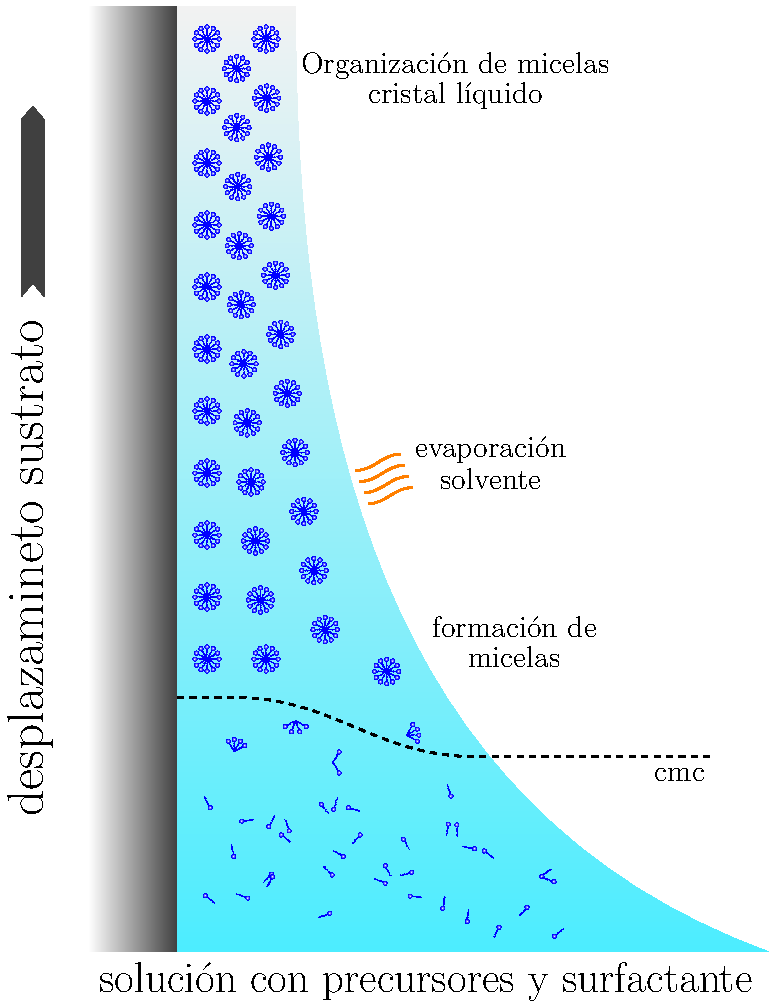
\includegraphics[width=0.5\textwidth]{Esquemas/autoensam.pdf}
 				\caption[Proceso de autoensamblado inducido por evaporación\index{autoensamblado inducido por evaporación} (AEIE\index{AEIE})]{Proceso de autoensamblado inducido por evaporación\index{autoensamblado inducido por evaporación} (AEIE\index{AEIE}) mediante \textit{dip-coating}\index{dip-coating@\textit{dip-coating}}. La evaporación del solvente favorece la formación de micelas mas allá de la cmc formado el cristal líquido\index{cristal líquido}. Un proceso similar ocurre cuando se aplica la técnica de \textit{spin-coating}\index{spin@\textit{spin-coating}}}
 		   		\label{fig:autoensam}
 		    	\end{center}
 		    	\end{figure}
	
   	En función de la composición inicial del sol, del tipo de surfactante\index{surfactante}, de la química de los precursor\index{precursor}es, del sustrato\index{sustrato} y de las condiciones ambientales es posible obtener diferentes condiciones que darán lugar a distintos arreglos tridimensionales de poros, que está dado por el organización micelar previo al momento en el cual se elimina el surfactante\index{surfactante} ya sea por calcinación\index{calcinación} o extracción\index{extracción}.\cite{Grosso2004,Grosso2002,Crepaldi2002a,Grosso2003,Violi2015} 
	



	%\subsection{Aplicaciones}
		%“Los materiales porosos pueden servir como anfitriones de catalizadores o como vehículos para transportar fármacos y realizar una liberación controlada de moléculas específicas”, señala la investigadora. La porosidad\index{porosidad} también es útil para modificar las propiedades intrínsecas de los materiales.
	 	
	 	%En concreto, el grupo de investigación de Paula Ferreira desarrolla materiales porosos en diversas formas y composiciones y destinados a diferentes aplicaciones. “Realizamos materiales porosos híbridos en los que integramos moléculas orgánicas con óxido de silicio\index{silicio!oxido de}\index{silicio} para capturar y separar gases”, comenta, así como “catálisis heterogénea y adsorción\index{adsorción} de contaminantes en el agua”.
		%Usos comerciales y en que formas, NP, materiales, sectores de aplicaciones. Low K.
\section{Sensores electroquímico\index{electroquimico}s\index{electroquimico}}
		

			
		Una vez elegido el campo de aplicación de los sensores\index{sensor} se debe pensar en adaptar o elegir procesos de fabricación adecuados, de forma de poder escalar la producción y transferirlo a la industria.

\section{Miniaturización y escalabilidad}\label{sec:microfabricacion}\label{sec:intro_fotolito}
		

		Como se mencionó anteriormente, las técnicas más usadas hoy en día para fabricar sensores\index{sensor} a gran escala, rentables y de pequeñas dimensiones son las conocidas como <<técnicas de microfabricación\index{microfabricación}>>, basadas en la aproximación \textit{top-down}\index{top-down@\textit{top-down}}. 

		La industria de los semiconductores es la que impulsa la ciencia y el desarrollo detrás de estos procesos. Hoy en día es claramente una industria madura, de enormes proporciones y de las mas rentables del mundo, productora de computadoras, celulares, tabletas, acelerómetros, giroscópos, sistemas de posicionamiento global, etc. Dicha industria se puede dividir en dos grandes grupos: en la industria de los micro/nano sistemas eléctrico mecánicos (MEMS\index{MEMS}/NEMS, del ingles \textit{Micro/Nano Electric Mechanicals Systems}) o en la de los circuitos integrados (IC, del ingles \textit{integrated circuit}). Al\index{aluminio} primer grupo pertenecen dispositivos como sensores, actuadores y controladores y al segundo grupo los microprocesadores y memorias que se basan casi exclusivamente en una unidad de mínima de procesamientos compuesta por transistores.

		Una de las claves del continuo crecimiento de esta industria durante las ultimas 40 años fue el desarrollo del procesamiento del silicio\index{silicio} y la tecnología planar. Trece años mas tarde de la invención del primer transistor (de germanio y de varios unos \SI{7}{\cm} de alto) por la compañía \textit{Bell Telephone Company}, en 1947, se crea, en 1960 el primer transistor planar, basado en silicio\index{silicio} y en procesos difusivos de impurezas sobre discos de silicio\index{silicio} monocristalinos. A partir de este hito tecnológico el número de transistores por oblea\index{oblea} de silicio\index{silicio} se duplica aproximadamente cada 18 meses. 
		
		Mediada la década de los 90 la industria de los semiconductores se sumerge en la nanotecnología\index{nanotecnología}, no por las nuevas propiedades que pueden surgir, sino por la necesidad de integración y de hacer dispositivos más densos, con mayor cantidad de componentes por unidad de área. La miniaturización permite obtener dispositivos cada vez más  veloces, que funcionan a mayores frecuencias, con menor disipación de potencia y a un menor costo. Todos estos requerimientos o necesidades tecnológicas se fueron materializando en un mercado de una capital enorme, que a su vez, se nutre de la industria, la cual se basa en la evolución de las técnicas y procesos de microfabricación\index{microfabricación}.

		En términos generales, se pueden resumir la fabricación para tecnologías basadas en silicio\index{silicio} en un proceso cíclico que comprende al menos una técnica de depósito\index{depósito} y una de transferencia de los diseños\index{transferencia!de los diseños}\index{transferencia!de los diseños}, denominada fotolitografía\index{fotolitografía} o litografía\index{litografía} óptica. El esquema de la figura \ref{fig:micro-intro} resume y ejemplifica alguna de las etapas que se pueden desarrollar durante la fabricación de un microsistema.
		
 			\begin{figure}[th!]
 				\begin{center}
 				\includegraphics[width=\textwidth]{Esquemas/micro-intro.pdf}
 				\caption[Etapas de los procesos de microfabricación\index{microfabricación}]{asdasdasdsa}
 		   		\label{fig:micro-intro}
 		    	\end{center}
 		    	\end{figure}

		En la fabricación de los dispositivos que se presentan en este trabajo se utilizó litografía\index{litografía} con lámpara de mercurio para la transferencia de los diseño, y pulverización catódica\index{pulverización catódica} como técnica para el depósito\index{depósito} de los electrodos.

		\subsection{Fotolitografía}

		Dentro del proceso de fabricación, la etapa de litografía\index{litografía} es una de las más criticas. Además esta etapa suele ser la que define la resolución de línea que se puede obtener. Mientras menor la longitud de onda\index{longitud de onda}\index{longitud de onda} empleada mas pequeños serán los motivos sensibles de ser transferidos. El nodo tecnológico queda definido por el tamaño de este motivo que suele hacer referencia al ancho del canal en un transistor.

		Los equipos comerciales dedicados a investigación y desarrollo (como el que se encuentra en el INTI\index{INTI}, ver sección \ref{sec:fotolito}, pág. \pageref{sec:fotolito}) suelen utilizar lamparas de Hg ($\lambda\index{longitud de onda}=$\SI{350}{\nm}) alcanzando resoluciones apenas por debajo del micron, y los dedicados a producción utilizan fuentes de emisión dentro del UV\index{UV} profundo, iluminando con $\lambda\index{longitud de onda}=$\SI{193}{\nm}. Con esta longitud de onda\index{longitud de onda}\index{longitud de onda} corta, utilizando líquidos de inmersión, corrimiento de máscara\index{máscara} y correcciones ópticas se llegan a definir detalles tan pequeños como \SI{32}{\nm}.







		\subsection{Pulverización catódica (\textit{sputtering})}



		%Triangulo virtuosos  
% %``''Todo deberia hacerse tan simple como sea posible, pero no mas que eso``'' Einsten.

% %\url{https://www.ted.com/talks/george_whitesides_toward_a_science_of_simplicity?language=es}\cite{ted_whitesides2010}
% Portabilidad

% \section{Microfabricacion}\label{sec:microfabricacion}

% Porque se elijio Au, Electroquimica, etc.

% Sputt: explicar sputt, fotolito porque microelectronica, MEMS\index{MEMS}, sensores.
% En los casos que se depositó la capa dieléctrica de SiO$_2$ se hizo con la fuente de radiofrecuencia\index{radiofrecuencia} (RF), mientras que los depósitos de las películas metálicas se realizaron con la fuente de corriente directa (DC), ambas configuradass a potencia constante, a P=\SI{400}{\watt}.  De esta forma se deja libre la tensión y la corriente, parámeros que dependen a su vez del vacío en la cámara, de la distancia entre el cátodo\index{cátodo} y el ánodo\index{anodo @ ánodo} y el caudal de argón\index{argón}.\cite{sigmund1968}. 

% \subsection{Fotolitografia}\label{sec:intro_fotolito}

% \subsection{sputtering}

% \section{implementacion tecnologica}
% nanotecnologia\cite{Gimenez2017}
% Intergrar bottom-up, top-down y hacer un dispositivo intergrado, miniaturizado, escalado, industrializable, tecnologicamente compatible, IC, logica, sensores\index{sensor} MEM
% Integracion, todo en argentina, valor agregado del proceso sol-gel\index{sol-gel}.\cite{Volksen2010}

% \section{Aplicaciones}

%\section{Electroquímica en películas delgadas mesoporosas}



\section{Motivaciones y objetivos}

	El presente trabajo de tesis se desarrolló en el Instituto Nacional de Tecnología Industrial (INTI), cuyas principales actividades son: certificación de productos, metrología industrial, científica y legal, y generación y transferencia	de innovación tecnológica a la industria. Es, dentro de este contexto, que surge el desafío de desarrollar un dispositivo en base nanotecnologica con posibilidad de ser transferido . 

	El objetivo principal de la tesis es desarrollar una plataforma de sensores\index{sensor} electroquímico\index{electroquimico}s\index{electroquimico} basados en películas delgadas mesoporosas. Las etapas y objetivos intermedios para la fabricación de los sensores\index{sensor} se pueden resumir en los siguientes ítems:

	\begin{itemize}
		
		\item Depositar y condensar películas delgadas mesoporosas de óxidos de silicio\index{silicio} estructuradas con F127 y CTAB sobre silicio, películas delgadas de oro\index{oro} y microelectrodo\index{electrodo!microelectrodo}s.  
		
		\item Desarrollar métodos para condensar la estructura inorgánica (óxidos de silicio\index{silicio} y silicio/circonio) y extraer el agente moldeante\index{agente moldeante} a temperaturas menores a los \SI{150}{\celsius}, de forma de evitar temperaturas de calcinación\index{calcinación}. 

		\item Compatibilizar procesos de síntesis \textit{bottom-up}\index{bottom-up@\textit{bottom-up}} con técnicas de microfabricación\index{microfabricación} tipo \textit{top-down}\index{top-down@\textit{top-down}}. Mejorar adherencia, minimizar procesos difusivos y evitar condiciones agresivas de condensación\index{condensación}.

		\item Estudio de propiedades de transporte, calculo de parámetros característicos mediante experimentos de electroquímica\index{electroquimico} y simulación\index{simulacion} computacional por métodos de elementos finitos\index{metodo de elementos finitos@método de elementos finitos}.

		\item Miniaturizacion de los sensores, estudios de escalabilidad, optimización de los diseños y pruebas electroquímica\index{electroquimico}s\index{electroquimico} funcionales.

		\end{itemize}	

	Finalmente cabe destacar, que este proyecto tiene por propósito, a mediano/largo plazo, fabricar una plataforma de sensores\index{sensor} analíticos selectivos incorporando nanotecnología\index{nanotecnología}, portable, integrable en circuitos integrados, de bajo costo y con posibilidades de ser transferido a la industria.
  %Linea Para poder completar automaticamente las citas con el Sublime
%No hace el documento, se puede borrar esta linea si no se usa el Sublime
%------------------------------------------------------------------------------
 \newcommand{\NoBiblioMat}[1]{
 \ifthenelse{\equal{#1}{verdadero}}{}{\bibliography{Referencias/base_bibliografica}}
 \NoBiblioMat{verdadero}}
 %-----------------------------------------------------------------------------

%Formato (Nombre de capitulo largo o corto), nombre del capitulo y estilo de la
%Portada del Capitulo
%------------------------------------------------------------------------------

 %Formato en si, titulo en un solo renglon
 \FormatoCapituloUnaLinea

 %Nombre y etiquete para referir
 \chapter{Materiales, Métodos y Procesos}\label{chap:Materiales}

 %Para que no salga el numero de pagina en la portada del capitulo
 \thispagestyle{empty}
	
 %Resumen del Capitulo en Italica 
  \noindent\textit{En este capitulo se presenta la descripción experimental de todos los materiales, instrumental y procesos involucrados en la tesis. En la primera sección se detallan los procesos de síntesis de las películas mesoporosas, desde la preparación de los soles\index{sol} hasta la caracterización de las mismas; en la segunda se presentan los procesos de fabricación de los electrodos, desde el diseño a las técnicas de transferencia; la tercera sección describe las técnicas de microscopia\index{microscopía}s utilizadas y la última sección detalla como se llevaron a cabo las mediciones electroquímica\index{electroquimico}s\index{electroquimico}.}


 %Indice de capitulo alineada al borde inferior de la pagina, nueva pagina
 \vfill
 \minitoc
 \newpage

 %-------------------------------------------------------------------------------

\section{Síntesis de películas delgadas mesoporosas}\label{sec:sintesis_mesoporosos}	
	
	 Las consideraciones teóricas sobre la química sol-gel\index{sol-gel} y el autoensamblado inducido por evaporación\index{autoensamblado inducido por evaporación} (AEIE\index{AEIE}) ya fueron expuestas en el capítulo \ref{chap:Introduccion}. También fueron mencionadas las razones por las cuales se eligió SiO$_2$ como estructura para las películas delgadas mesoporosas y Pluronic F127\index{Pluronic F127} o CTAB como agente moldeante\index{agente moldeante}. Los procedimientos, métodos y proporciones molares para la preparación de los soles\index{sol} fueron, en su mayoría, adaptaciones de los trabajos de Angelomé\index{Angelomé}\cite{Angelome2008} y Fuertes\index{Fuertes}\cite{Fuertes2009}. El esquema \ref{esq:peliculas_meso} resume cada etapa de síntesis de las películas, que se explican con detalle en las próximas secciones.
		  \begin{figure}[ht]
			  \begin{center}
			  \includegraphics[width=\textwidth]{Esquemas/Resumen_sintesis_meso.pdf}
			  \caption[Síntesis de películas delgadas mesoporosas]{Diagrama de flujo para la síntesis de películas delgadas mesoporosas.}
			  \label{esq:peliculas_meso}
			  \end{center}
			  \end{figure}
			  \vspace*{-0.2cm}

	\subsection{Preparación de los soles, reactivos y nomenclatura}\label{sec:soles}
		
			La síntesis y depósito\index{depósito} de las películas delgadas mesoporosas comienzan con la preparación de las soluciones, las cuales deben contener los precursor\index{precursor}es del óxido (o de los óxidos en el caso de películas mixtas), el agente moldeante\index{agente moldeante} de los poros, solvente adecuado, H$_2$O y HCl\index{acido@ácido!clohídrico}\cite{Brinker1990}. Cada uno de estos componentes cumple una función especifica, tal como se explicó en la sección \ref{sec:mesoporosos}. Los precursor\index{precursor}es utlizados fueron tetraetoxisilano\index{tetraetoxisilano} (TEOS, \textit{Merck}) para las películas de sílice pura, y TEOS combinado con cloruro de circonio(IV) (ZrCl$_4$, \textit{Aldrich}) para las películas mixtas de silicio/circonio. Las condiciones de hidrólisis\index{hidrolisis@hidrólisis} y condensación\index{condensación} para estos dos reactivos (ya sean solos o combinados) son bien conocidas y llevan a la formación películas delgadas estables y reproducibles de óxidos mesoporosos puros o mixtos\cite{Soler-Illia2004,Crepaldi2002a,Angelome2008}. El surfactante\index{surfactante} es el agente que establece el tamaño de los poros, se utilizó para ello el copolímero de bloque Pluronic F127\index{Pluronic F127} (F127, \textit{Aldrich}) y bromuro de hexadeciltrimetilamonio\index{bromuro de hexadeciltrimetilamonio} (CTAB, \textit{Aldrich}). Como solvente se utilizó etanol\index{etanol} absoluto (EtOH, \textit{Sigma}). El H$_2$O es el reactivo para la formación del óxido mediante la conexión de los grupos metálicos M(IV). Por último, el HCl\index{acido@ácido!clohídrico} es el encargado de generar el medio ácido\index{acido@ácido} que cataliza la hidrólisis\index{hidrolisis@hidrólisis} y controla la condensación\index{condensación} del Si(IV) y/o del Zr\index{circonio}(IV). Los reactivos utilizados fueron de calidad proanalisis o superior y el H$_2$O de \SI{18}{\mega\ohm\per\cm} fue obtenida con un equipo \textit{Ultra Clear TWF} de la marca \textit{Siemens}. La nomenclatura, pesos moleculares y estructura química de los reactivos utilizados se pueden consultar en la tabla \ref{tabla:reactivos}.
					
			El preparado de las soluciones se realizó agregando cada reactivo por pesada en balanza analítica. Cada lote de solución fue de aproximadamente \SI{100}{\ml}. Para llegar a este volumen se agregaron, en este orden, \SI{10.417}{\gram} de TEOS, \SI{6.911}{\gram} de etanol\index{etanol} y \SI{0.902}{\gram} de HCl\index{acido@ácido!clohídrico} \SI{2,77e-3}{\Molar}. En el caso de los soles\index{sol} mixtos (Si/Zr 9:1), se pesaron \SI{9.375}{\gram} de TEOS y \SI{1.165}{\gram} de Zr\index{circonio}Cl$_4$. Esta primera solución, denominada solución de prehidrólisis, se deja envejecer bajo agitación constante durante \SI{48}{\hour} a \SI{25}{\celsius}, con el objetivo de hidrolizar los precursor\index{precursor}es metálicos y mantener un bajo grado de condensación\index{condensación}.\cite{Grosso2001}

				\begin{table}[ht!] 
						  \caption[Reactivos para los soles]{Nomenclatura, estructura, peso molecular y función de las moléculas utilizadas en las soluciones para la síntesis de películas delgadas mesoporosas.} 
				  		  \begin{tabular}{>{\raggedright\arraybackslash}m{2.40cm}>{\centering\arraybackslash}m{4cm}>{\centering\arraybackslash}m{2.35cm}>{\raggedright\arraybackslash}m{1.7cm}} 
				  		  \toprule
						  Nombre Nomenclatura    & Estructura & Peso molecular \si{g.mol^{-1}} & Función\\ \midrule
				      	  tetraetoxisilano\index{tetraetoxisilano} TEOS & \includegraphics[scale=0.5]{Esquemas/teos.pdf} & $208,33$ & precursor\index{precursor} del óxido  \\ \midrule
				      	  \mbox{cloruro de circonio(IV)}  Zr\index{circonio}Cl$_4$ & \includegraphics[scale=0.8]{Esquemas/zrcl4.pdf} & $233.04$ & precursor\index{precursor} del óxido  \\ \midrule
				  		  Pluronic F127\index{Pluronic F127} F127    & \hspace*{-10px} 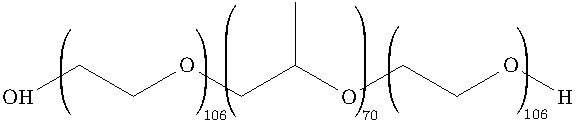
\includegraphics[scale=0.5]{Esquemas/f127.pdf} & \multirow{1}{*}{$13800$}	 & agente moldeante\index{agente moldeante}	 \\ \midrule
				  		  bromuro de hexadeciltrimetilamonio\index{bromuro de hexadeciltrimetilamonio}  CTAB   & \hspace*{1cm} 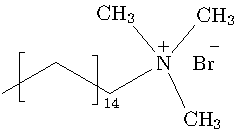
\includegraphics[scale=0.6]{Esquemas/ctab.pdf} & \multirow{1}{*}{$364.48$}	 & agente moldeante\index{agente moldeante}	 \\ \midrule
				  		  ácido\index{acido@ácido} clohídrico\index{acido@ácido!clohídrico} HCl\index{acido@ácido!clohídrico}& \includegraphics[scale=0.75]{Esquemas/hcl.pdf}  & \multirow{1}{*}{$36,46$}   & cataliza la hidrólisis\index{hidrolisis@hidrólisis} \\ \midrule
				  		  agua \hspace{2cm} H$_2$O  &  \includegraphics[scale=0.75]{Esquemas/agua.pdf}  & \multirow{1}{*}{$18,02$}   & reactivo de hidrólisis\index{hidrolisis@hidrólisis} \\ \midrule
				  		  etanol\index{etanol} \hspace{2cm} EtOH\index{etanol}  & \includegraphics[scale=0.75]{Esquemas/etanol.pdf}  & \multirow{1}{*}{$46,07$}   & solvente \\ 
				  		  \bottomrule
				    	  \end{tabular}
				   		  \label{tabla:reactivos}
					      \end{table}

			Una vez envejecida la solución de prehidrólisis\index{prehidrólisis} (ya sea de SiO$_2$ pura o mixta) se agregan a \SI{17.146}{\gram} de esta, \SI{80.184}{\gram} de EtOH\index{etanol}, \SI{3.246}{\gram} de F127 o \SI{1.822}{\gram} de CTAB y \SI{7.630}{\gram} de HCl\index{acido@ácido!clohídrico} \SI{2,5e-2}{\Molar}. De esta forma se obtienen unos \SI{100}{\ml} de un sol\index{sol} con las relaciones molares de la tabla \ref{tabla:soles}. Se conservan en \textit{frezeer} a \SI{-18}{\celsius} y sólo se retiran a la hora de depositar las películas. 

			Para facilitar la lectura se utilizará la siguiente nomenclatura, tanto para los soles\index{sol} como para las películas delgadas mesoporosas que se fabriquen con ellos: 

				\begin{itemize}
			 			\item \pdm\space para películas delgadas mesoporosas en general.
			 			\item \pdmF\space para \pdm\space de óxido de silicio\index{silicio!oxido de}\index{silicio} estructuradas con F127. 
			 			\item \pdmC\space para \pdm\space de óxido de silicio\index{silicio!oxido de}\index{silicio} estructuradas con CTAB.
			 			\item \pdmZ\space para las \pdm\space mixtas de óxido de circonio\index{circonio} y silicio\index{silicio} en relación molar $1\!:\!9$ y estructuradas con F127. 
					    \end{itemize}	
			
			Todas las soluciones fueron preparadas indistintamente en el Centro de Micro y Nanoelectrónica del Bicentenario del Instituto Nacional de Tecnología Industrial (INTI-CMNB) o en la Gerencia Química, Centro Atómico Constituyentes Comisión Nacional de Energía Atómica (CAC-CNEA). 
					
				\begin{table}[h!]
			  		  \caption[Relación molares de los soles]{Relaciones molares para las soluciones utilizadas.} 
			  		  \begin{tabular}{>{\raggedright\arraybackslash}m{2.2cm}>{\centering\arraybackslash}m{2.2cm}>{\centering\arraybackslash}m{1.875cm}>{\centering\arraybackslash}m{1.875cm}>{\centering\arraybackslash}m{1.875cm}} 
			  		  \toprule
					  Componente & Prehidrólisis  & \pdmF   & \pdmC  & \pdmZ \\  \midrule
			      	  TEOS 		  & 1/0,9$^*$	  & 1   	& 1		 & 0,9   \\ \midrule
			      	  Zr\index{circonio}Cl$_4$	  & -/0,1$^*$	  &	-		& - 	 & 0,1   \\ \midrule	
			      	  EtOH\index{etanol} 		  & 3			  & 40   	& 40	 & 40    \\ \midrule
			      	  F127 		  & -		 	  & 0,0075  & -		 & 0,0075\\ \midrule
			      	  CTAB 		  & -             & -		& 0,1	 & 0,1   \\ \midrule
			      	  H$_2$O	  & 1			  & 9	  	& 9	     & 9     \\ \midrule
			      	  HCl\index{acido@ácido!clohídrico}    	  & 0,00005		  & 0,01   	& 0,01	 & 0,01   \\ 
			      	  \bottomrule
			    	  \end{tabular}\vspace*{2pt}
		    	  	  \footnotesize{$^*$Los números después de la barra son los utilizados en soluciones de prehidrolisis para películas mixtas de silicio/circonio.}
			    	  \label{tabla:soles}
			   		  \end{table}

	\subsection{Depósitos de las películas delgadas mesoporosas}\label{sec:deposito_pdm}

			Las películas mesoporosas utilizadas en esta tesis fueron depositadas en el Laboratorio de Fotolitografía del INTI\index{INTI}-CMNB por \textit{spin-coating}\index{spin@\textit{spin-coating}}. La técnica consiste en un portamuestras acoplado a un cabezal rotatorio que al girar dispersa el líquido para formar una película sobre el sustrato.

			Como sustrato\index{sustrato} para realizar los depósitos se utilizaron: vidrio, silicio, oro\index{oro} sobre silicio, microelectrodo\index{electrodo!microelectrodo}s y sustratos poliméricos como  polimetilmetacrilato (PMMA) y poliestireno\index{poliestireno} de alto impacto (PAI). Cada uno de ellos fue escogido para una función particular (p. ej. sustrato\index{sustrato} para reacciones electroquímica\index{electroquimico}s\index{electroquimico}) o por alguna característica distintiva (p. ej. transparente en el IR). En la tabla \ref{tabla:sustratos}, pág. \pageref{tabla:sustratos}, se agrupan los sustratos utilizados y se resumen algunas características y funciones destacadas.

			Las dimensiones de las muestras fueron típicamente de \SI{1x1}{\cm} a \linebreak \SI{2x2}{\cm}, aunque la técnica permite depositar películas continuas de hasta \SI{15}{cm} de diámetro. En algunos casos, para obtener lotes de 32 o 46 sensores\index{sensor} (dependiendo del diseño), se utilizaron obleas de silicio\index{silicio} de \SI{10}{\cm} de diámetro. Antes de hacer el depósito, el sol\index{sol} se pasa a través de un filtro de jeringa\index{jeringa} de nailon de \SI{0.45}{\um} (\textit{GAMAFIL}) para evitar la presencia de partículas que puedan generar discontinuidades y/o <<cometas>> en los depósitos\cite{Franssila2004}. Luego, para dispensar el sol\index{sol} en el sustrato, se utilizaron pipetas tipo Pasteur\index{Pasteur} o pipetas automáticas dependiendo del volumen requerido, el cual varió de 80 a \SI{100}{\uL.\cm^{-2}}. Las condiciones del laboratorio durante el depósito\index{depósito} se mantuvieron en \SI{25}{\celsius} y a una HR entre 30\% y 50\%. Una vez dispensado el sol, se da comienzo a la rotación que dispersa la solución de manera homogénea sobre el sustrato\index{sustrato} y, a su vez, la evaporación del solvente promueve la formación del cristal líquido\index{cristal líquido} por el mecanismo de AEIE\index{AEIE}\cite{Brinker1999}.


			El espesor\index{espesor} de la película, ($t$), es inversamente proporcional a la raíz cuadrada de la velocidad angular\index{velocidad!angular} ($\omega$), es decir $t\propto \omega ^{-1/2}$. Las rampas de velocidad y aceleración fueron optimizadas para obtener \pdm\space con espesor\index{espesor}es entre 150 y \SI{300}{\nm}\cite{Meyerhofer1978,Hall1998,Brinker1990}. Los esquemas aplicados se muestran en gráfico de la figura \ref{fig:rampa-spin}. 
				
					
			 	    \begin{table}[ht!]
			  		   \caption[Sustratos utilizados para el depósito\index{depósito} de \pdm]{Sustratos utilizados para el depósito\index{depósito} de \pdm.} 
			  		   \begin{tabular}{>{\raggedright\arraybackslash}m{2.4cm}>{\raggedright\arraybackslash}m{2.5cm}>{\raggedright\arraybackslash}m{2cm}>{\raggedright\arraybackslash}m{3.55cm}} 
			  		   \toprule
					   Sustrato Nomenclatura   & Observaciones  & Limpieza previa$^*$ & Función \\ \midrule
			       	   vidrio\index{vidrio} \hspace{2cm} Vi  &	portaobjetos \textit{BioTraza} & inmersión KOH 40\% & económico para pruebas preliminares de depósito\index{depósito} \\ \midrule
			       	   silicio\hspace{2cm} Si  & Si[100] pulido dopado tipo n  \textit{Addison}& inmersión HF\index{acido@ácido!fluohídrico} 48\% & FTIR, MEB, FIB\index{FIB}, PEA \\ \midrule
			       	   Au\index{oro} sobre silicio\hspace{2cm} Si$|$Au & depositado por pulverización catódica\index{pulverización catódica}$^\dagger$  & ultrasonido\index{ultrasonido}en H$_2$O  & transporte, EQ\\ \midrule
			      	   microelectrodo\index{electrodo!microelectrodo}s \hspace{2cm} $\mu Elec$ & sensores, diseño transferido por fotolitografía\index{fotolitografía}$^\mathsection$  	  &  ultrasonido\index{ultrasonido}en H$_2$O  & multisensado, EQ \\ \midrule
			      	   poliméricos         &  PMMA y PAI		  &  ultrasonido\index{ultrasonido}en H$_2$O &  demostrador métodos suaves de síntesis\\ 
			      	   \bottomrule
			    	   \end{tabular}\vspace*{2pt}
			    	   \footnotesize{$^*$Ver la sección <<\nameref{sec:limpieza}>>, tabla \ref{tabla:limpieza}, pág. \pageref{sec:limpieza}.}\\
			    	   \footnotesize{$^\dagger$Ver la sección <<\nameref{sec:sputt}>>, pág.\pageref{sec:sputt}.} \\
			    	   \footnotesize{$^\mathsection$Ver la sección <<\nameref{sec:fotolito}>>, pág. \pageref{sec:sputt}.}
			    	   \label{tabla:sustratos}
			   		   \end{table}

			   		   \begin{figure}[!ht]
						 \begin{center}
						 \includegraphics[width=0.70\textwidth]{Graficos/rotacion_meso.pdf}
						 \caption[Parámetros de depósito\index{depósito} para las \pdm]{Esquema con las rampas más frecuentes de aceleración, velocidad y tiempo utilizadas para el depósito\index{depósito} de \pdm.}
						 \label{fig:rampa-spin}
						 \end{center}
						 \end{figure}
			
			 El equipo utilizado fue un \textit{Suss MicroTec Delta 20BM}, el cual consiste en un cabezal rotatorio con control de aceleración (0 a  \SI{1000}{\minute^{-1}.\second^{-1}}) y velocidad angular\index{velocidad!angular} (0 a \SI{10000}{\minute^{-1}}). Posee múltiples portamuestras para sustratos de diferentes tamaños con entrada de vacío para sujetar las muestras (figura \ref{fig:spin}).   		   

					\begin{figure}[ht!]
					  \begin{center}
					  \includegraphics[width=\textwidth]{Imagenes/Spin.jpg}
					  \caption[Equipo para el depósito\index{depósito} de películas delgadas, \textit{spin-coater}]{\textit{Spin-coater} ubicado en el Laboratorio de Fotolitografía del INTI\index{INTI}-CMNB utilizado para el depósito\index{depósito} de las películas delgadas mesoporosas, Marca \textit{Suss MicroTec}, modelo \textit{Delta 20BM}.}
					  \label{fig:spin}
					  \end{center}
					  \end{figure}

	\subsection{Eliminación del surfactante\index{surfactante}}\label{sec:cond_y_extr}

		Una vez realizado el depósito, se debe conservar la estructura del cristal líquido\index{cristal líquido} obtenido, y evitar el deterioro durante la eliminación\index{eliminación} del surfactante\index{surfactante}. Para ello se estabiliza la película durante \SI{1}{\hour} en cámara de humedad controlada a una HR constante de 50\%. Para mantener dicho valor de humedad se utilizó una solución saturada de Ca(NO$_3$)$_2$.5H$_2$O (\textit{Biopack}). Controlar la presión parcial de agua (P$_{\text{H}_2\text{O}}$) permite optimizar el grado de condensación\index{condensación} del óxido y ayuda a la separación de fases entre el agente moldeante\index{agente moldeante} y el óxido\cite{Crepaldi2003}. El proceso de estabilización y condensación\index{condensación} del óxido continua con un calentamiento en plancha calefactora, (\textit{Cimarec}) una hora a \SI{60}{\celsius} y una hora más a \SI{130}{\celsius}\cite{Crepaldi2003,Crepaldi2002a}. 
				
		Posteriormente a la estabilización de la película se experimentaron varios tratamientos para completar el proceso de condensación\index{condensación} de la fase inorgánica y extraer el surfactante\index{surfactante} para dar lugar a la película nanoporosa, a saber:

				\begin{itemize}

				\item \textit{Calcinacion.} Este es el proceso clásico en el cual se somete a la película a una temperatura de \SI{350}{\celsius} durante \SI{2}{\hour} con una rampa de \SI{1}{\celsius.\minute^{-1}} (Horno \textit{Indef 337}). De esta forma se condensa el óxido, se elimina el surfactante\index{surfactante} y se minimiza el daño de la estructura tridimensional de la red nanoporosa\index{película!nanoporosa} \cite{Crepaldi2003}.

				\item \textit{Condensación ácida.} En este método se busca promover la condensación\index{condensación} de la matriz inorgánica mediante la exposición de las películas a una atmósfera de vapores de HCl\index{acido@ácido!clohídrico} \cite{Doshi2000a}. El arreglo para tal fin consiste en sujetar las muestras al fondo de un vaso de precipitados y colocarlo invertido sobre un cristalizador con HCl\index{acido@ácido!clohídrico} concentrado (\textit{Biopack}) durante \SI{10}{\minute}. 

				\item \textit{Condensación alcalina.} Al\index{aluminio} igual que el método anterior, se busca promover la condensación\index{condensación} del óxido cambiando las condiciones del entorno químico, en este caso someter las películas a una atmósfera de pH\index{pH} alcalino generada con vapores de NH\index{amoniaco}$_3$ (\textit{Biopack}) \cite{Soler-Illia2012,Soler-Illia2011}. El armado experimental fue igual que el descripto para el método ácido.

				\item \textit{Tratamiento a \SI{130}{\celsius}.} Esta estrategia de síntesis involucró dejar las muestras en estufa a \SI{130}{\celsius} durante 7 días con el objetivo de promover la condensación\index{condensación} del óxido.

				\item \textit{Alto vacío.} Este tratamiento consiste en dejar las muestras en una cámara de alto vacio\index{alto@alto vacío} a \SI{1e-5}{\milli\bar} y \SI{130}{\celsius} durante 7 días. Para calentar y llegar al vacío necesario se utilizó la cámara de una soldadura de obleas (\textit{EVG 501 Manual Wafer Bonding System}) la cual fue evacuada por una bomba mecánica y una turbomolecular secuencialmente.

				\end{itemize}
					
		En los casos donde fue necesario realizar la extracción\index{extracción} del surfactante\index{surfactante} sin calcinar, las muestras fueron sometidas a un reflujo\index{reflujo} de isopropanol\index{propanol@2-propanol} a punto de ebullición (\textit{Biopack}) durante \SI{15}{\minute}. Luego se enjuagaron con H$_2$O acidificada con HCl\index{acido@ácido!clohídrico} a $\text{pH}=2$. El siguiente diagrama de flujo resume y agrupa los tratamientos realizados sobre las \pdm, desde el depósito\index{depósito} hasta la extracción\index{extracción} del surfactante\index{surfactante}.
		
				\begin{figure}[ht!]
						  \begin{center}
						  \includegraphics[width=\textwidth]{Esquemas/Resumen_extraccion.pdf}
						  \caption[Tratamientos pos-depósito de \pdm]{Etapas de estabilización y diferentes tratamientos pos-depósito utilizados para condensar las \pdm\space, tanto de óxidos puros como las mixtas y extraer el surfactante\index{surfactante}.}
						  \label{esq:peliculas_meso_tratamientos}
						  \end{center}
						  \end{figure}

	\pagebreak \subsection{Espectroscopia IR}\label{sec:IR}

		La región infrarroja (IR) del  espectro electromagnético\index{espectro electromagnético} puede ser divido en tres zonas, según su longitud de onda\index{longitud de onda}\index{longitud de onda}, IR cercano (400 a \SI{10}{\cm^{-1}}), IR medio (4000 a \SI{400}{\cm^{-1}}), e IR lejano (14000 a \SI{4000}{\cm^{-1}}). El infrarrojo medio puede ser usado para estudiar las vibraciones\index{vibración} fundamentales y la estructura roto-vibracional; brinda información acerca de los grupos funcionales orgánicos y la estructura inorgánica a través del análisis de las vibraciones\index{vibración} moleculares.\cite{Atkins2006,Barrow1962,Stuart2004} 
		
		A lo largo de este trabajo se uso esta porción del espectro IR para analizar los resultados de la extracción\index{extracción} de surfactante\index{surfactante} y estructura inorgánica de las \pdm. Las mediciones se llevaron a cabo en la Unidad Técnica de Nanomateriales del Centro de Investigaciones en Procesos Superficiales del INTI\index{INTI} (INTI-CIEPS). El equipo es un \textit{Thermo Scientific Nicolet 6700 FTIR} que cuenta con un microscopio para poder focalizar el haz en un área de aproximadamente \SI{0.5x0.5}{\mm}. Se utilizó la técnica de espectroscopia\index{espectroscopia} infrarroja por transformadas de Fourier (FTIR) tanto en trasmisión como en reflexión y los espectros fueron tomados con el detector MCT/B (\textit{Wide Band mercury cadmium telluride}) que es de 4 a 10 veces más sensible que los detectores estándar para equipos de espectroscopia\index{espectroscopia} FTIR.\cite{Nicholet2007} Las películas destinada a ser caracterizadas por FTIR\index{FTIR} fueron depositadas sobre Si, por ser éste trasparente en el IR medio.

	\subsection{Ángulo de contacto}

		Medir el ángulo de contacto\index{angulo@ángulo de contacto} (AC) de un líquido permite evaluar la energía\index{energía} superficial ($\gamma$). La teoría vincula el AC coni $\gamma$ mediante el análisis del equilibrio químico de tres fases. La fase líquida de la gota, la fase gaseosa del aire y la sólida del sustrato. El valor del AC depende principalmente de la relación que existe entre las fuerzas adhesivas entre el líquido y el sólido y las fuerzas cohesivas del líquido. Se puede, así, cuantificar la mojabilidad\index{mojabilidad} de un líquido en aire, en una determinada superficie\index{superficie}.\cite{findenegg1997} Tomando dos caso extremos, cuando la superficie\index{superficie} interactúa fuertemente con el líquido y se moja, el AC se aproxima a $0^{\circ}$, en cambio si la superficie\index{superficie} y el líquido se repelen, el AC tenderá a $180^{\circ}$. En términos de equilibrio termodinámico, el potencial químico de las tres fases  debe ser igual. Quien dió la primera descripción en términos de energías interfasiales fue Young\index{Young} en 1805\cite{young1805}, donde postuló que la energía\index{energía} superficial líquido-vapor ($\gamma$) por el coseno del angulo de contacto($\theta$) es igual a diferencia de las energías superficiales sólido-líquido $\gamma_{_{SL}}$ y sólido-vapor $\gamma_{_{SV}}$s. Tal relación se la conoce como ecuación de Young\index{Young} (ecuación \ref{eq:young}).

			\begin{equation}
				\gamma\, cos(\theta) = \gamma_{_{SL}} - \gamma_{_{SV}}
				\label{eq:young} 
				\end{equation}

		En este trabajo se utilizaron las medidas de AC entre agua y las superficie\index{superficie}s de las \pdm, para calcular la distribución de los tamaños de poro\index{poro} y cuello\index{cuello de poro} de los sistemas porosos aplicando la ecuación de Kelvin\index{Kelvin}.\cite{Boissiere2005} En la próxima sección se explica en detalle como se estiman dichas distribuciones.
		Las medidas de AC se realizaron en la Gerencia Química, CAC-CNEA con un equipo \textit{Ramé-Hart 290} y los datos fueron recogido con el software \textit{DROPImage}.

	\subsection{Elipsometría}\label{sec:elipso}

		La elipsometría es una técnica de análisis óptico que se basa en el cambio del estado de polarización\index{polarización} de la luz que incide sobre una o más películas delgadas soportadas sobre un material reflectivo. Dicho análisis es no destructivo y es útil para la determinación de espesor\index{espesor}es y constantes ópticas (índices de refracción y constante de absorción) de dichas películas.\cite{TompkinsHarlandG.1999,Rothen1945} El parámetro medido es el cociente complejo $\rho$ de la amplitud de la reflexión de los componentes paralelo ($r_p$) y perpendicular ($r_s$) del haz polarizado incidente. Este cociente se expresa como función de los parámetros elipsométricos $\Delta(\lambda\index{longitud de onda})$ y $\Psi(\lambda\index{longitud de onda})$. 

		Debido a que las ecuaciones involucradas en el proceso no poseen resolución analítica, es necesario recurrir a modelos que describan el material para obtener las propiedades de interés, es decir, el índice de refracción\index{indice@índice de refracción} real, $n$, el espesor\index{espesor}, $t$, y el coeficiente de absorción\index{coeficiente de absorción} $k$. Mediante un ajuste iterativo por cuadrados mínimos de $\Delta(\lambda\index{longitud de onda})$ y $\Psi(\lambda\index{longitud de onda})$ (para el cual se proponen valores iniciales para $n$, $k$ y $t$ de la muestra) se minimiza la diferencia ente el modelo y los datos experimentales. De esta forma se extrae el espesor\index{espesor} y el índice de refracción\index{indice@índice de refracción}. \cite{TompkinsHarlandG.1999}

		Cuando se adapta al equipo una cámara, en la que se puede variar la presión parcial de H$_2$O, es posible medir los cambios de las propiedades ópticas (p. ej. espesor\index{espesor} e índice de refracción\index{indice@índice de refracción}) de las \pdm\space durante la adsorción\index{adsorción} y desorción\index{desorción} de H$_2$O. A esta técnica se la conoce con el nombre de porosimetría elipsométrica ambiental (PEA) \cite{Boissiere2005}. La figura \ref{fig:elipso} muestra un esquema de los principales componentes de un elipsómetro con cámara de humedad controlada.

			  \begin{figure}[h]
				\begin{center}
				\includegraphics[width=\textwidth]{Esquemas/Elipso.pdf}
			  	\caption[Esquema de la técncia de elipsoporosimetría\index{elipsoporosimetría ambiental} ambiental]{Esquema de los componentes principales del equipos de elipsometría utilizado para determinar las constantes elipsométricas, $\Delta(\lambda\index{longitud de onda})$ y $\Psi(\lambda\index{longitud de onda})$, de las cuales se obtienen el espesor\index{espesor}, indice de refracción, coeficiente de absorción\index{coeficiente de absorción},  distribución y tamaño de poro\index{distribución!de poro}s y cuello\index{cuello de poro}s de las \pdm.}
			  	\label{fig:elipso}
			  	\end{center}
			  	\end{figure}
		
		El volumen de vapor adsorbido dentro de los poros se determina a partir de la variación de $n(\lambda\index{longitud de onda})$ utilizando aproximaciones de medio efectivo como la de Bruggeman\index{Bruggeman}\cite{Bruggeman1935} o la de Maxwell-Garnett\index{Maxwell-Garnett}\cite{Garnett1906} que son simplificaciones de la ecuación Lorentz-Lorentz\index{Lorentz-Lorentz}  general\cite{TompkinsHarlandG.1999}.
		La aproximación de Bruggeman\index{Bruggeman} considera dos componentes mezclados al azar cuyas fracciones en volumen ($f_i$) y constante dieléctrica\index{constante dieléctrica} ($\mathcal{E}_i$) deben cumplir con la ecuación \ref{eq:bruggeman} donde $\mathcal{E}_e$ es la constante dieléctrica\index{constante dieléctrica} del material compuesto. El índice de refracción\index{indice@índice de refracción} se define según la ecuación \ref{eq:indice} donde $\mu$ es permeabilidad electromagnética relativa.
		
						\begin{equation}
					 	   n=\sqrt{\mathcal{E}\mu}
					 	   \label{eq:indice}
						\end{equation}
		
		\pagebreak 

		Para la mayoría de los materiales, y cerca del rango visible, $\mu$ es muy cercana a la unidad, por lo tanto es común aproximar $\mathcal{E}_e=n_e^2$.
							\begin{equation}
					 		   	 f_1\left(\frac{\mathcal{E}_1-\mathcal{E}_e}{\mathcal{E}_1+2\mathcal{E}_e}\right)+
					 		   	 f_2\left(\frac{\mathcal{E}_2-\mathcal{E}_e}{\mathcal{E}_2+2\mathcal{E}_e}\right)=0
					 		     \label{eq:bruggeman}
								\end{equation}
		La aproximación de Maxwell-Garnett\index{Maxwell-Garnett} considera al material compuesto por al menos dos especies, la matriz y la inclusión. En el caso de los óxidos porosos, la matriz es el óxido y el aire el surfactante\index{surfactante} la inclusión. Se deben satisfacer en este caso las ecuaciones \ref{eq:maxwall1} y \ref{eq:maxwall2}.
				
							\begin{equation}
					 		   	 f_1\left(\frac{\mathcal{E}_1-\mathcal{E}_2}{\mathcal{E}_1+1\mathcal{E}_2}\right)-
					 		   	 \left(\frac{\mathcal{E}_e-\mathcal{E}_2}{\mathcal{E}_e+2\mathcal{E}_2}\right)=0
					 		     \label{eq:maxwall1}
								\end{equation}
						
								\begin{equation}
					 		   	 f_2\left(\frac{\mathcal{E}_2-\mathcal{E}_1}{\mathcal{E}_1+2\mathcal{E}_1}\right)-
					 		   	 \left(\frac{\mathcal{E}_e-\mathcal{E}_1}{\mathcal{E}_e+2\mathcal{E}_1}\right)=0
					 		     \label{eq:maxwall2}
								\end{equation}
		
		El volumen total ocupado por los poros, V$_p$, y el volumen de agua adsorbido para cada HR, V$_{ads}$, se calcularon aplicando indistintamente dichas aproximaciones (ya que para \pdm\space dan resultados equivalentes) a las constantes dieléctricas\index{constante dieléctrica} (o índices de refracción) medidas del film seco y lleno de agua, luego de la condensación\index{condensación} capilar.\cite{Angelome2008,Fuertes2009,Nano-compuestas2013}. Se construye de esta forma una isoterma\index{isoterma} de adsorción\index{adsorción}/desorción de H$_2$O en función del índice de refracción\index{indice@índice de refracción} (o volumen poroso) de las películas porosas. Los distintos tipos de isortermas para la adsorción\index{adsorción} de sobre materiales absorbentes porosos fue clasificada por la IUPAC\index{IUPAC} en ocho grupos (Ia, Ib, II, III, IVa, IVb, V y VI) y seis ciclos de histéresis\index{histéresis} para los tipos IVa y V (H1, H2a, H2b, H3, H4 y H5). \cite{Thommes2015}

		La figura \ref{fig:pea_ej}a muestra un resultado típico para adsorción\index{adsorción} de agua en una película de óxido de silicio\index{silicio!oxido de}\index{silicio} estructurada con CTAB medida por PEA. La curva resultante corresponde a una isoterma\index{isoterma} tipo IVa/H2b. El ciclo de histéresis\index{histéresis} indica la presencia de mesoporos, cuyo llenado se produce por condensación\index{condensación} capilar. \cite{Gregg1967}La gran mayoría de las isoterma\index{isoterma}s obtenidas fueron de este tipo (IVa con ciclo H2b) y, consecuentemente, son las más dicutidas y analizadas a lo largo de este trabajo. 

			\begin{figure}[!ht]
		     	  		\begin{subfigure}[t]{0.491\textwidth}
		     	  		\includegraphics[width=\textwidth]{Graficos/CTAB_M2_Modelo_isoterma.pdf}
						\label{fig:pea_ej1}
						\end{subfigure}
						\begin{subfigure}[t]{0.495\textwidth}
		     	  		\includegraphics[width=\textwidth]{Graficos/CTAB_M2_Modelo_distribucion.pdf}
						\label{fig:pea_ej2}
						\end{subfigure}
						\vspace*{-0.6cm}
						\caption[Isoterma de adsorción\index{adsorción}/desorción tipo IVa, H2b.]{(a) Isoterma de adsorción\index{adsorción}/desorción de agua para un sistema mesoporosos de SiO$_2$ estructurado con CTAB. La misma se clasifica según la IUPAC\index{IUPAC} como tipo IVa con ciclo de histéresis\index{histéresis} H2b; (b) Distribución de tamaño de poro\index{poro} y cuello\index{cuello de poro}.}
						\label{fig:pea_ej}
						\end{figure}			
		\vspace{0.3cm}				
		Se puede calcular a partir de las ramas de adsorción\index{adsorción} y desorción\index{desorción} de la isoterma\index{isoterma} la distribución para los diámetros de poros y cuello\index{cuello de poro}s respectivamente. Los resultados que se obtienen son similares al ejemplo de la figura \ref{fig:pea_ej}b. Para realizar este cálculo debemos recurrir a la ecuación de Kelvin\index{Kelvin} (ec. \ref{eq:kelvin}), que describe el equilibrio líquido-vapor considerando el tamaño de la esfera y la energía\index{energía} superficial. Donde R es la constante de los gases, T es la temperatura, P es la presión de vapor\index{presión de vapor}, P$_s$ es la presión de vapor\index{presión de vapor} de saturación, $\gamma$ es la tensión superficial\index{tensión superficial} del líquido, V$_m$ es el volumen molar del líquido y $\theta$ es el ángulo de contacto\index{angulo@ángulo de contacto} sólido-líquido. \cite{Baklanov2000,Boissiere2005,Sing1985} Para poros esféricos la relación $\partial S/ \partial dV$ es proporcional al radio de la esfera, llamado radio de Kelvin\index{Kelvin}.\cite{FernandezPrini2005}
		
			\begin{equation}
			  	 \ln \left(\frac{P}{P_s}\right)=\frac{2\gamma V_m}{RT} \cos{\theta}\frac{\partial S}{\partial V}
			     \label{eq:kelvin}
			 	 \end{equation}					
	
		Todas las medidas fueron tomadas en la Gerencia Química, CAC-CNEA con un elipsómetro espectroscópico marca \textit{SOPRA}, modelo \textit{GES 5E}. El rango espectral del equipo va de 190 a \SI{900}{\nm}, pose una cámara para realizar las mediciones en condiciones de humedad controlada y también permite configuración en modo \textit{micro-spot} que permite reducir el área de medición a una región de aproximadamente \SI{1}{\mm^2}. El modelado de los parámetros se hizo mediante el \textit{software Winelli II} también de la marca \textit{SOPRA}.
			
						% \begin{figure}[ht]
						% 	  \begin{center}
						% 	  \includegraphics[width=\textwidth]{Imagenes/elipsometro.jpg}
						% 	  \caption[Elipsómetro]{Foto del equipos elipsómetro espectroscópico marca \textit{SOPRA}, modelo \textit{GES 5E} ubicado en la Gerencia Química, CAC-CNEA utilizado para la caracterización de las \pdm.}
						% 	  \label{fig:elipsofoto}
						% 	  \end{center}
						% 	  \end{figure}

\section{Microfabricación de los electrodos}
		
	 En esta sección se dará cuenta de los detalles experimentales para la fabricación de los electrodos, los cuales son una parte fundamental de los sensores. Es en la superficie\index{superficie} de los electrodos donde se llevan a cabo las reacciones de óxido-reducción de los analitos de interés y donde se depositan la película delgada \index{película!delgada}mesoporosa. Por estos motivos resulta fundamental contar con un diseño funcional y compacto y, además, controlar los aspectos superficiales tales como la rugosidad\index{rugosidad}, control de impurezas, espesor\index{espesor}, y funcionalización en los caso que sea necesario.

	 \begin{figure}[h!]
			  \begin{center}
			  \includegraphics[width=0.85\textwidth]{Esquemas/Resumen_micro.pdf}
			  \caption[Esquema para la transferencia de los diseños\index{transferencia!de los diseños}\index{transferencia!de los diseños}]{Diagrama general para la transferencias y fabricaciones de diseños de una o más capas. Este esquema contempla el uso de las técnicas de \textit{lift-off }o grabado según se requiera dependiendo de las características de los materiales empleados para esa capa.}
			  \label{esq:micro}
			  \end{center}
			  \end{figure}

	 Los electrodos fueron enteramente diseñados y fabricados en los laboratorios del CMNB-INTI. 
		
	 Las herramientas y técnicas empleadas para la fabricación son propias del sector de la microelectrónica\index{microelectrónica}; herramientas de \textit{software}\index{software@\textit{software}} tipo CAD, fotolitografía\index{fotolitografía}, pulverización catódica\index{pulverización catódica}, grabado por vía húmeda, \textit{lift-off}\index{lift@\textit{lift-off}}, corte y encapsulado, etc.\cite{Franssila2004,Jaeger2001} Cada uno de estos procesos y metodologías se explicarán en las secciones subsiguientes. 

	 El flujo general de trabajo para la transferencias de diseños en una o más capas se presenta en la figura \ref{esq:micro}.
			  
	\subsection{Diseño e impresión de las máscara\index{máscara}s}\label{sec:impresion_mascaras}

		El primer paso necesario en la fabricación de los sensores\index{sensor} es el diseño. Como todo diseño en microelectrónica\index{microelectrónica}, se diagramó en función de las tecnologías disponibles, de la calidad de las máscara\index{máscara}s y de la aplicación final en la cual se emplearán. Todos estos aspectos ya fueron expuestos en el capitulo \ref{chap:Introduccion}, por lo que aquí nos remitiremos a describir los detalles técnicos.

		Los diseños fueron realizados para obleas de \SI{10}{\cm} de diámetro. El primer diseño se mandó a imprimir en filmina\index{filmina} de \SI{13x13}{\cm} en una filmadora de películas \textit{Agfa Accuset 1000}, a una resolución de \SI{3600}{dpi}, perteneciente a la firma $Imacrom$. Esto ha permitido obtener resoluciones de linea de \SI{50}{\um}, muy por encima de la resolución de la tecnología de la cual disponemos (transferencia por UV, $\lambda\index{longitud de onda}=365nm$). El segundo diseño, mas completo e integrado, también fue diagramado para obleas de \SI{10}{\cm} de diámetro. Éste contempló la integración del contraelectrodo\index{electrodo!contraelectrodo} y el electrodo de referencia\index{electrodo!de referencia}, además de incluir 6 electrodos de trabajo\index{electrodo!de trabajo}. Las máscara\index{máscara}s correspondientes a este diseños se mandaron a imprimir en filmina\index{filmina}s de \SI{13x13}{\cm} a la empresa \textit{International Phototool Company} a una resolución de \SI{48000}{dpi}, logrando mejor resolución y lineas más definidas que en el primer diseño, hasta de \SI{7}{\um}. Todos los diseños se llevaron a cabo con el \textit{software CAD electric}\index{software@\textit{software}!\textit{electric}} (\url{http://www.staticfreesoft.com/productsFree.html}) de licencia pública general de GNU, \url{https://www.gnu.org/licenses/gpl.html}. 
				
	\subsection{Limpieza de los sustratos}\label{sec:limpieza}
			
			Una vez terminado el diseño, comienza la etapa de transferencia del mismo. El primer paso es la limpieza de los sustratos para evitar problemas de falta de adhesión y eliminar impurezas superficiales adsorbidas. 

			\begin{table}[!ht]
					  \caption[Soluciones para la limpieza de los sustratos]{Soluciones utilizadas para hacer la limpieza antes de realizar cualquier proceso de fotolitografía\index{fotolitografía} o pulverización catódica\index{pulverización catódica}.\cite{Franssila2004,Kern1990}}
			  		  \begin{tabular}{>{\raggedright\arraybackslash}m{1.02cm}>{\centering\arraybackslash}m{2.8cm}>{\centering\arraybackslash}m{1.9cm}>{\centering\arraybackslash}m{1.9cm}>{\raggedright\arraybackslash}m{2.4cm}} 
			  		  \toprule
					  Nombre  & Composición &  Proporciones & Condiciones & Blanco \\ \midrule
			      	  KOH$^*$ & KOH:H$_2$O 	&    40\%p/v    &  \SI{25}{\celsius}/\SI{10}{\minute}  &  residuos orgánicos \\  \midrule
			      	  SC1$^\dagger$ &	H$_2$O:H$_2$O$_2$:NH\index{amoniaco}$_4$OH & 5:1:1 & \SI{80}{\celsius}/\SI{10}{\minute} & residuos orgánicos  \\ \midrule
			      	  SC2 &	H$_2$O:H$_2$O$_2$:HCl\index{acido@ácido!clohídrico} & 6:1:1 & \SI{80}{\celsius}/\SI{10}{\minute}   &  residuos iónico\index{iónico}s y metálicos \\ \midrule
			      	  HF\index{acido@ácido!fluohídrico}  &	H$_2$O:HF & 50:1 & \SI{25}{\celsius}/\SI{2}{\minute} & óxido de silicio\index{silicio!oxido de}\index{silicio} \\ \midrule
			      	  iPOH    &	  (CH$_3)_2$CHOH &  puro$^\mathsection$      &  enjuague & residuos grasos \\ \midrule
			      	  H$_2$O & H$_2$O desionizada & puro$^\ddagger$  &  enjuague  & desorción\index{desorción} de partículas \\ \midrule
			      	  Piraña &  H$_2$SO$_4$:H$_2$O$_2$ & 2:1 & \SI{25}{\celsius}/\SI{10}{\minute}  & residuos orgánicos  \\
			      	  \bottomrule
			    	  \end{tabular}
			    	  \footnotesize{$^*$}No apta para silicio, racciona con el mismo para formar Si(OH)$_4$ e H$_2$. \\
				      \footnotesize{$^\dagger$}Crece una capa de SiO$_2$ de 10 a \SI{15}{\angstrom} de espesor\index{espesor}. \\
				      \footnotesize{$^\mathsection$}Grado analítico o superior. \\
			    	  \footnotesize{$^\ddagger$}Resistividad de \SI{18}{\mega\ohm\per\cm} o mayor.
			    	  \label{tabla:limpieza}
			   		  \end{table}
			
							
			La tabla \ref{tabla:limpieza} resume cuales fueron las soluciones utilizadas para limpieza, su composición y cuál es la finalidad de cada una. Al\index{aluminio} finalizar cada etapa de limpieza siempre se hace un lavado con H$_2$O DI seguido de un secado con aire o N$_2$. El porqué de los materiales elegidos para usar de sustratos ya fueron discutidos en el capitulo \ref{chap:Introduccion}, aquí solo se mencionan los protocolos de limpieza\cite{Franssila2004,Kern1990} utilizados para cada uno de ellos:

				\begin{itemize}
					\item{Vidrio: KOH}
					\item{Silicio: SC1, SC2, HF\index{acido@ácido!fluohídrico} o piraña\index{piraña} según el caso}
					\item{Sustratos poliméricos: ipOH}
				\end{itemize}

    \subsection{Transferencia de los diseños por fotolitografía\index{fotolitografía}}\label{sec:fotolito}

		La transferencia de los diseños\index{transferencia!de los diseños} se realizó por fotolitografía\index{fotolitografía}, técnica que también se conoce con los nombres de litografía\index{litografía} óptica o litografía\index{litografía} ultravioleta\index{UV} (UV). La técnica consiste en depositar una resina fotosensible sobre un sustrato, irradiar con luz UV\index{UV} de $\lambda\index{longitud de onda}\!=$\SI{365}{nm} a través de una máscara\index{máscara} y por último revelar la fotorresina\index{fotorresina}. Dependiendo si esta es negativa, positiva o de doble exposición, se disolverá la parte expuesta (positiva) o la no expuesta a la luz (negativa). \cite{Jaeger2001,Franssila2004,Mack2007,Mack2006}
				

			  \begin{figure}[b!]
			  \begin{center}
			  \includegraphics[width=0.70\textwidth]{Esquemas/fotolito.pdf}
			  \caption[Esquema fotolitografía\index{fotolitografía}]{Proceso de fotolitografía\index{fotolitografía} para una resina de doble exposición\index{resina!de doble exposición}. 1) Deposito de la resina, 2) Calentamiento suave, mejora la adherencia\index{adherencia} y evapora solventes, 3) 1$a$ exposición, 4) Calentamiento para invertir la polaridad de la resina, 5) 2$a$ exposición sin máscara\index{máscara}, 6) Revelado, notese el perfil invertido, especialmente útil para aplicar en procesos de\textit{ lift-off}.}
			  \label{esq:fotolito}
			  \end{center}
			  \end{figure}	

		Antes de depositar la fotorresina\index{fotorresina} se calienta el sustrato\index{sustrato} hasta \SI{120}{\celsius} con el objetivo de desorber H$_2$O. Los depósitos de las resinas se realizaron mediante \textit{spin-coating}\index{spin@\textit{spin-coating}} con el equipo descrito en la sección \ref{sec:deposito_pdm}, pág. \pageref{sec:deposito_pdm}. Para cubrir una oblea\index{oblea} completa de \SI{10}{\cm} de diámetro se necesitan colocar un mínimo de \SI{5}{\ml} de fotorresina\index{fotorresina} \textit{TI35E image reversal} de la marca \textit{Microchemicals}, la cual es de doble exposición, especialmente elegida por formar un perfil negativo, particularmente útil para el proceso \textit{lift-off}\index{lift@\textit{lift-off}}, explicado mas adelante.\cite{MicrochemicalsTeam2009} 
	
		El deposito se hizo por \textit{spin-coating}\index{spin@\textit{spin-coating}}, a una velocidad final de \SI{4000}{\minute^{-1}} durante \SI{40}{\second}, con una aceleración de \SI{400}{\minute^{-1}.\second^{-1}} para obtener un espesor\index{espesor} final de \SI{4}{\um}. Luego se realiza un calentamiento durante \SI{2}{\minute} a \SI{95}{\celsius} para evaporar el exceso de solvente y promover la adhesión de la resina al sustrato. Seguidamente se cargan el sustrato\index{sustrato} y la máscara\index{máscara} en la alineadora\index{alineadora} de máscara\index{máscara}s (\textit{EVG 620}, figura \ref{fig:alineadora}), la cual cuenta con un microscopio incorporado para hacer la alineación máscara\index{máscara}/sustrato y una lámpara de Hg para el sistema de irradiación UV\index{UV} ($\lambda\index{longitud de onda}=$\SI{365}{\nm}). 
			\begin{figure}[b!]
			  \begin{center}
			  \vspace*{-0.4cm}%Para que entre la imagen de la pagina siguiente del sputt
			  \includegraphics[width=\textwidth]{Imagenes/alineadora.jpg}
			  \caption[Alineadora de máscara\index{máscara}s]{Alineadora de máscara\index{máscara}s \textit{EVG 620} semiautomática de doble cara, con lámpara de Hg de \SI{350}{W}  y capacidad para obleas de hasta \SI{150}{\mm} .}
			  \label{fig:alineadora}
			  \end{center}
			  \end{figure}	
			
		Después de alinear, se realiza la primera exposición con una densidad de energía\index{energía!densidad de}\index{energía} de \SI{140}{mJ.\cm^{-2}} y se deja reposar \SI{10}{\minute} para dar tiempo a la difusión\index{difusión} de N$_2$ liberado durante la reacción. Se realiza ahora el calentamiento para invertir el perfil (las zonas expuestas polimerizan volviéndose inerte al solvente) de la resina a una temperatura de \SI{120}{\celsius} durante \SI{2}{\minute}  y se expone por segunda vez a una densidad de energía\index{energía!densidad de}\index{energía} de \SI{540}{mJ.cm^{-2}}, esta vez sin máscara\index{máscara}. En esta segunda exposición las partes polimerizadas no se afectan, mientras las no expuestas en la primera iluminación se vuelven solubles en el medio revelador. Para finalizar, se hace el revelado\index{revelado} sumergiendo la oblea\index{oblea} en un cristalizador con una solución de revelador\index{revelador} \textit{AZ General} (\textit{Microchemicals}) y H$_2$O 1:1. La evolución del revelado\index{revelado} se siguió mediante microscopia\index{microscopía}\index{microscopía!óptica} y se determinó el tiempo óptimo de inmersión en aproximadamente unos \SI{7}{\minute}, dependiendo del espesor\index{espesor} de la fotoresina. De esta forma quedan transferidos los diseños. El flujo de trabajo se sintetiza en el esquema \ref{esq:fotolito}.
			 
	\subsection{Depósito películas delgadas metálicas}\label{sec:sputt}

			En esta sección se describe el proceso de fabricación de las películas delgadas de Au, cuya función es ser usadas como electrodos en los sensores. Las mismas se depositaron utilizando técnica de pulverización catódica\index{pulverización catódica}, la cual es comúnmente conocida por su nombre en ingles, \textit{sputtering}\index{sputtering@\textit{sputtering}}\cite{sigmund1968}. Los fundamentos básicos de la técnica se discutieron en el capitulo \ref{chap:Introduccion}, pág. \pageref{sec:microfabricacion}.
							
			Los sustratos utilizados para depositar los electrodos fueron principalmente obleas de silicio\index{silicio} monocristalinas (vírgenes o fotolitografiadas) y portaobjetos de vidrio. Estos soportes fueron elegidos debido la baja rugosidad\index{rugosidad} de su superficie\index{superficie} y por ser materiales que pueden ser sometidos a temperaturas altas, en particular \SI{350}{\celsius}, que es la temperatura de calcinación\index{calcinación} para la ruta de síntesis clásica de óxidos mesoporosos. Previo a realizar el depósito, los sustratos fueron tratados con los procesos de limpieza descritos en la sección \ref{sec:limpieza}, pág. \pageref{sec:limpieza} y una vez dentro de la cámara se realizó una limpieza por plasma para promover una mayor adherencia\index{adherencia} del depósito\index{depósito} al sustrato.

			Cabe destacar que si se trabaja sobre obleas de silicio, estas tienen que estar recubiertas con una capa dieléctrica para que no haya fugas eléctricas a través del silicio. A lo largo de este tesis se utilizó indistintamente obleas que ya venían con capa aislante u obleas a las cuales se le depositó una película delgada \index{película!delgada}de SiO$_2$, también por pulverización catódica\index{pulverización catódica}.

			Para promover la adherencia\index{adherencia} del Au, se deposita una capa de al menos \SI{20}{\nm} de espesor\index{espesor}, indistintamente de Ti\index{titanio} o Cr\index{cromo}. Sin esta capa, el Au\index{oro} no adhiere sobre superficie\index{superficie}s no metálicas\cite{Hieber1976}. Una vez depositada esta capa de adherente y sin romper el vacío de la cámara del equipo, se depositan un mínimo \SI{150}{\nm} de Au, para lograr un electrodo mecánicamente robusto y con buenas propiedades de conducción eléctrica. En los casos que se depositó una capa dieléctrica de SiO$_2$ se utilizó la fuente de radiofrecuencia\index{radiofrecuencia} (RF) a potencia constante, P=\SI{400}{W}. Mientras que los depósitos de las películas metálicas se realizaron todos con la fuente de corriente directa (DC) también configurada a P=\SI{400}{W}, dejando la tensión y la corriente libre, parámetros que dependen a su vez del vacío en la cámara, de la distancia entre el cátodo\index{cátodo} y el ánodo\index{anodo @ ánodo} y el caudal de argón\index{argón}. 

			
			Las condiciones óptimas de depósito\index{depósito} de cada una de las capas se detallan en las tablas \ref{tabla:sputt1} y \ref{tabla:sputt2} . La primera contienen las condiciones para las películas metálicas y la segunda para la película de SiO$_2$ y el proceso de limpieza por plasma previo a los depósitos. Manteniendo las condiciones experimentales constantes se construyó, para cada material, una curva de calibración del espesor\index{espesor} en función del tiempo de depósito. De esta forma se obtuvieron las tasas de depósitos que figuran en la última columna en las tablas \ref{tabla:sputt1} y \ref{tabla:sputt2}, esencial para controlar el espesor\index{espesor} de cada películas. Las mediciones de espesor\index{espesor}es se realizaron mediante microscopia\index{microscopía} FIB\index{FIB}, técnica que se describe en la sección \ref{sec:micros}.

			%Tabla con los parámetros de deposito de la películas
		  		\begin{table}[ht]
		  		\caption[Parámetros de depósito\index{depósito} películas metálicas]{Parámetros de depósito\index{depósito} de las distintas películas delgadas metálicas para su uso como electrodos de trabajo\index{electrodo!de trabajo}.}
		  		\begin{tabular*}{\textwidth}{c @{\extracolsep{\fill}} lcccccc} 
		  		\toprule
		    	 Depósito&$P_{_{\text{DC}}}$(W) & $T$(V)  &  $I$(A)   & $p$(mbar) & $Q_{Ar}$(sccm) & $T$(nm/min) \\
		    	 		\midrule
		  		 Ti\index{titanio} 	 & $400$ & $750$ & $0.53$ & \num{1.70e-3} & $5$ & $50$ \\
		  		 Cr\index{cromo} 	 & $400$ & $453$ & $0.84$ & \num{1.70e-3} & $5$ & $55$ \\
		  		 Au\index{oro} 	 & $400$ & $679$ & $0.56$ & \num{1.35e-3} & $5$ & $44$ \\
		    	 \bottomrule
		    	 \end{tabular*}
		   		\label{tabla:sputt1}
		   		\end{table}
		   		\vspace{-0.6cm}
		  		\begin{table}[ht]
		  		\caption[Parámetros de depósito\index{depósito} películas dieléctricas]{Parámetros de depósito\index{depósito} utilizado para el depósito\index{depósito} de $SiO_2$.}
		  		\begin{tabular*}{\textwidth}{c @{\extracolsep{\fill}} lccccc} 
		  		 		\toprule
		       	Depósito&$P_{_{\text{RF}}}$(W)  &$P_{ref}$(W)  &$p$(mbar) & $Q_{Ar}$(sccm) &$T$(nm/min)\\
		    	 		\midrule
		  		 $SiO_2$  & $400$ & $23$ & \num{1.23e-2} & $80$ & $1.18$ \\
		  		 Limpieza & 150   & 3    & \num{2.04e-3} & 10   & -      \\
		  		\bottomrule
		  		\end{tabular*}
		   		\label{tabla:sputt2}
		   		\end{table}
		   	
		   	Todos los depósitos fueron realizados en el equipo de \textit{sputtering}\index{sputtering@\textit{sputtering}} del INTI\index{INTI}-CMNB. El mismo cuenta, entre sus principales capacidades, con una fuente DC (hasta \SI{1.5}{\kW}) una fuente de RF (\SI{600}{W} a \SI{13.56}{\MHz}), posibilidad de depositar 3 materiales consecutivamente y capacidad para colocar sustratos de hasta \SI{250}{\nm}. El mismo es de la marca \textit{Boc Edwards}, en la figura \ref{fig:sputt} se muestra el equipo y un detalle al momento de hacer los depósitos.

		   		  \begin{figure}[b!]
				  \begin{center}
				  \includegraphics[width=\textwidth]{Imagenes/sputt.jpg}
				  \caption[Equipo para depósito\index{depósito} de películas delgadas, \textit{sputtering}\index{sputtering@\textit{sputtering}}]{Foto del instrumental utilizado para realizar los depósitos bicapa Ti\index{titanio}\textbar Au\index{oro} o Cr\index{cromo}\textbar Au.(A) El equipo \textit{BOC Edwards} completo donde se ve el gabinete de control y la cámara de vacío, (B) Foto a través de la ventana al momento de realizar un deposito de Cr\index{cromo} y (C) Foto a través de la ventana al momento de realizar un deposito de Au.}
				  \label{fig:sputt}
				  \end{center}
				  \end{figure}

	\subsection{Proceso de\textit{ lift-off}}

   	     Una vez finalizados los procesos de fotolitografía\index{fotolitografía} y pulverización de cada una de las capas es necesario remover el excedente de material. Este proceso de remoción, que se explica aquí, se conoce por su nombre en ingles \textit{lift-off}\index{lift@\textit{lift-off}}.

		 La bicapa Ti\index{titanio}\textbar Au\index{oro} o Cr\index{cromo}\textbar Au\index{oro} se pulverizó sobre toda la superficie\index{superficie} de la oblea, tanto en las partes donde estaba el silicio\index{silicio} descubierto como en las partes donde quedó la fotorresina\index{fotorresina} sin revelar. 
			
		 De esta forma, al estar el metal sobre la resina, disolviendo ésta, se desvincula la capa Ti\index{titanio}\textbar Au\index{oro} del sustrato\index{sustrato} y queda completa la transferencia de los diseños\index{transferencia!de los diseños}. 
		 La disolución de la fotoresina se lleva a cabo en acetona\index{acetona} (\textit{Sigma}) dentro de un baño de ultrasonido\index{ultrasonido}(\textit{TESTLAB} Modelo \textit{tb02}) a \SI{22}{\kHz}. En la figura \ref{esq:liftoff} se esquematiza todo el proceso completo.

		 \begin{figure}[h!]
			  \begin{center}
			  \includegraphics[width=\textwidth]{Esquemas/liftoff.pdf}
			  \caption[Esquema del proceso de\textit{ lift-off}]{Esquema del proceso de\textit{ lift-off} en el cual se solubiliza la fotorresina\index{fotorresina} con película metálica encima. 1) Fotorresina transferida en base a un diseño arbitrario, 2) depósito\index{depósito} metálico, 3) disolución de la fotorresina\index{fotorresina} con un solvente adecuado, 4) Diseño completamente trasferido.}
			  \label{esq:liftoff}\index{lift@\textit{lift-off}}
			  \end{center}
			  \end{figure}

	\subsection{Modificación superficial}\label{sec:silanizacion}
		
		A lo largo del trabajo surgió la necesidad de mejorar la adherencia\index{adherencia} de las \pdm\space sobre los electrodos de Au\index{electrodo!de Au}. Para lograr ésto, se realizó sobre los electrodos una modificación superficial, de forma de generar puntos de anclaje para promover la adherencia\index{adherencia} del óxido de silicio\index{silicio!oxido de}\index{silicio} sobre la superficie\index{superficie} de los electrodos.
		El proceso consistió en vincular covalentemente una molécula\index{moléculas} a la superficie\index{superficie} de Au\index{oro} y, por otro lado, que ésta misma molécula\index{moléculas} sea parte estructural de las \pdm. Para lograr ésto se preparó una solución \SI{10}{\milli\Molar} de 3-mercaptopropil trimetoxisilano\index{mercaptopropil@3-mercaptopropil trimetoxisilano} (MPTMS) en tolueno\index{tolueno} (se eligió tolueno\index{tolueno} de forma de minimizar la hidrólisis\index{hidrolisis@hidrólisis} y condensación\index{condensación} del MPTMS) y se dejó reaccionar durante 2 horas en cristalizador cubierto con un vidrio\index{vidrio} de reloj. \cite{Goss1991,Herzog2013} Luego se realiza un enjuague con acetona\index{acetona} y se seca en flujo de N$_2$.

	\subsection{Encapsulado y corte}\label{sec:corte}

		Sobre los electrodos depositados se deposita una resina negativa\index{resina!negativa}, epoxi\index{epoxi} y fotocurable, \textit{SU8-100} de \textit{MicroChemical}\cite{MicrochemicalsTeam2009}. Dicha resina es ópticamente transparente y de alta viscosidad, lo que permite generar capas de hasta \SI{100}{\um} de espesor\index{espesor}. 

		Fue utilizada con un doble propósito, proteger mecánicamente los sensores\index{sensor} y hacer un reservorio o celda con un volumen  $V \approx$ \SI{2}{\ul}, el cual contendrá la solución con los analitos que se desean detectar.  
			%Graficos de rampa de veloci\index{velocidad!rampa de}dades		  
			\begin{figure}[t!]
			 		  \begin{center}
			 		  \includegraphics[width=0.70\textwidth]{Graficos/rotacion_su8.pdf}
			 		  \caption[Parámetros de depósito\index{depósito} para la resina expoxi\index{resina!expoxi}\index{epoxi}]{Esquema de aceleración y velocidad de rotación\index{velocidad!de rotación} para el depósito\index{depósito} de la fotorresina\index{fotorresina} epoxi\index{epoxi} SU8.}
			 		  \label{fig:spin-su8}
			 		  \end{center}
			 		  \end{figure}
			
			\begin{figure}[b!]
			 		  \begin{center}
			 		  \includegraphics[width=\textwidth]{Imagenes/dicer.jpg}
			 		  \caption[Cortadora de obleas]{Cortadora de obleas de la marca \textit{Laser Optics}, ubicada en los laboratorios del INTI\index{INTI}-CMNB}
			 		  \label{fig:dicer}
			 		  \end{center}
			 		  \end{figure}
		
		Para controlar el espesor\index{espesor} mediante \textit{spin-coating}\index{spin@\textit{spin-coating}} se utilizó el esquema de rotación que de la figura \ref{fig:spin-su8}. Luego se realizó un secado para evaporar solventes a \SI{65}{\celsius} durante \SI{1}{\minute} y \SI{95}{\celsius} durante \SI{10}{\minute}. Seguidamente, se expone al UV\index{UV} a través de la máscara\index{máscara} con una densidad de energía\index{energía!densidad de}\index{energía} de \SI{680}{mJ.cm^{-2}}, para activar los iniciadores de la polimerización\index{polimerización} sólo en las zonas iluminadas. Se realiza un segundo calentamiento gradual de \SI{1}{\minute} a \SI{65}{\celsius} y \SI{12}{\minute} a \SI{95}{\celsius} para incrementar el grado de polimerización\index{polimerización} y finalmente se lleva a cabo el revelado\index{revelado} (revelador para resina SU-8 de \textit{MicroChemical}), el cual requiere un tiempo de \SI{10}{\minute} para disolver completamente las partes que no fueron expuestas a la luz UV. 
		
		Para concluir la fabricación de los sensores\index{sensor} se corta la oblea\index{oblea} en cuadrados de \SI{1x1}{\cm} con el propósito de obtener así cada dispositivo individual con 6 electrodos de trabajo\index{electrodo!de trabajo} cada uno. El corte se realiza con un disco de carburo de silicio\index{silicio} de la marca \textit{Loadpoint} a con una velocidad de rotación\index{velocidad!de rotación} de \SI{44000}{\minute^{-1}} y una de avance de \SI{0.5}{\mm\per\second}. El mismo fue montado en una cortadora de obleas marca \textit{Laser Optics} ubicada en los laboratorios del INTI\index{INTI}-CMNB (ver figura \ref{fig:dicer}).
	
	\subsection{Espectroscopia de fotoelectrones de rayos X\index{rayos Xssh}}

		La técnica de XPS\index{XPS} (del ingles, \textit {X-ray photoelectron spectroscopy}) es una espectroscopia\index{espectroscopia} semi-cuantitativa y de baja resolución espacial que habitualmente se utiliza para estimar la estequiometría, estado químico de oxidación de algún elemento en particular y la estructura electrón\index{electrón}ica de los elementos en superficie\index{superficie}.\cite{siegbahn1956,siegbahn1981}

		Se hizo uso de esta técnica para evaluar estados de oxidación del Au\index{oro} y comprobar difusión\index{difusión} de contaminantes hacia la superficie\index{superficie} de los electrodos.  Los equipos constan de diferentes componentes; una cámara de ultra alto vacio\index{alto@alto vacío} (UHV) con presiones del orden de \SI{1e-9}{mbar} para disminuir la cantidad de contaminantes superficiales y asegurar a los electrones eyectados un camino libre medio lo suficientemente grande como para alcanzar el analizador. La cámara está construida en acero inoxidable y posee ventanas de vidrio\index{vidrio} para poder observar su interior. A ella se acoplan diferentes elementos necesarios para el análisis superficial como la fuente de rayos X\index{rayos Xssh}, el analizador de electrones, el cañón de iones, entre otros.\cite{XPS1978,Corthey2012}

		Las medidas de XPS\index{XPS} realizadas se llevaron a cabo en el Instituto de Investigaciones Fisicoquímicas Teóricas y Aplicadas (INIFTA\index{INIFTA}). Se utilizó una fuente de Mg K$\alpha$ (\textit{XR50, Specs GmbH}) y un analizador hemisférico (\textit{PHOIBOS 100, Specs GmbH}). La presión dentro de la cámara de UHV fue menor a \SI{1e-9}{mbar}. El ángulo entre la fuente de rayos X\index{rayos Xssh} y el eje del analizador está fijado en \ang{54;44;00}. Los valores de sección eficaz de fotoionización están tabulados para esta geometría. Se realizó una calibración de la escala de energía\index{energía} de dos puntos utilizando Au\index{oro} evaporado ($E_B$ de Au$f_{7/2}$ = \SI{84}{\electronvolt}) y Cu ($E_B$ de Cu $2_{p3/2}$ = \SI{932.67}{\electronvolt}).
		
\section{Microscopías}\label{sec:micros}
		
	 En este apartado haremos un breve resumen de los tipos de microscopia\index{microscopía}s utilizadas durante la tesis.

	\subsection{Microscopía óptica}

		Se utilizó microscopia\index{microscopía}\index{microscopía}\index{microscopía!óptica} en modo reflexión, fundamentalmente para evaluar la superficie\index{superficie} (homogeneidad, fracturas, grietas, etc), tanto de las películas metálicas como de las mesoporosas. También para determinar la calidad de las máscara\index{máscara}s impresas y para establecer los tiempos de revelado\index{revelado} en los procesos fotolitográficos. Se hizo uso de un microscopio \textit{Olympus} modelo \textit{BX51} configurado tanto para trasmisión como para reflexión. Como fuente de luz el equipo cuenta con lámpara halógena y, en los casos que hizo falta, se intercaló un filtro ultravioleta\index{UV} de forma de no exponer las fotorresina\index{fotorresina}s durante la inspección y evaluación de los tiempos de revelado.
	
	\subsection{Microscopía electrón\index{electrón}ica de barrido (MEB)}\label{sec:SEM}

		La microscopia\index{microscopía}\index{microscopía} electrón\index{electrón}ica de barrido (MEB) nos permitió ver y caracterizar las películas delgadas, ya sean los electrodos o las \pdm. Tamaño de poro, homogeneidad, tamaño de cristales, microfisuras y espesor\index{espesor}es son algunas las características que se pudieron evaluar con esta técnica. Además, el equipo utilizado nos permitió hacer análisis por espectroscopia\index{espectroscopia} de rayos X\index{rayos Xssh} dispersiva en energía\index{energía} (EDS, del inglés \textit{Energy Dispersive Spectroscopy}) y tomar imágenes tanto de electrones secundarios como de electrones retrodifundidos. \cite{Goodhew2000,Watt1997}

		Todas las mediciones e imágenes fueron realizadas con un microscopio de doble haz de la marca \textit{FEI}, modelo \textit{Helios NanoLab 650} equipado con dos columnas, una de iones de galio\index{galio} y otra de electrones. Los iones producen cortes nanométricos y los electrones generan imágenes de alta resolución. La figura \ref{fig:sem-fib} muestra una fotografía del Laboratorio de Microscopía FIB\index{FIB} del CMNB-INTI donde se encuentra instalado el equipo. La fuente de la columna de electrones es un emisor tipo FEG (del ingles \textit{Field Emission Gun}) y como instrumental de detección cuenta con detector de electrones secundarios (SE, del ingles \textit{Secondary Electron}), de electrones retrodifundidos (BSD, del ingles \textit{back scatter detector}) y de inmersión (TLD, \textit{Thought Lens Detector}), ver esquema presentado en la figura \ref{esq:sem-fib}. 

				\begin{figure}[bh!]
			 		  \begin{center}
			 		  \includegraphics[width=\textwidth]{Imagenes/sem-fib.jpg}
			 		  \caption[Microscopio de doble haz FIB\index{FIB}/SEM]{Equipo de FIB\index{FIB}/SEM utilizados para realizar las observaciones, cortes y caracterizaciones de los sensores. Consta de un microscopio de barrido electrón\index{electrón}ico de alta resolución y de una fuente de galio\index{galio} líquido para realizar, entre otras cosas, cortes en la micro y nanoescala\index{nanoescala}.}
			 		  \label{fig:sem-fib}
			 		  \end{center}
			 		  \end{figure}
	
		Se utilizaron tensiones de trabajo bajas, típicamente entre \SI{1}{\kilo\electronvolt} y \SI{5}{\kilo\electronvolt} e intensidades del orden de los \SI{25}{\pA}. La justificación de estos valores es que al acelerar los electrones con bajas tensiones, la penetración en la muestra es pobre. Si bien depende del tipo de material, podemos estimar en base simulaciones de trabajos en la literatura especializada que, para oro\index{oro} o silicio, la penetración con los valores de tensión citados es de unos 50 a \SI{200}{\nm} \cite{Joy1984,Shur2012,Hafner2007}. Por el otro, se utilizó un flujo de electrones también bajo (\SI{25}{\pA}), de manera de evitar el apantallamiento debido a la acumulación de carga superficial en la muestra. Todos las imágenes de MEB en este trabajo incluyen las condiciones experimentales utilizadas en la barra de información situada debajo de cada una de ellas.

	\subsection{Microscopía con iones de galio\index{galio} focalizados (FIB)}\label{sec:FIB}

		El bombardeo con haz de iones (FIB, del ingles \textit{focused ion beam}) es una técnica que se utiliza fundamentalmente para el análisis de materiales en general, y en particular para materiales propios de la industria de la microelectrónica\index{microelectrónica}, más específicamente para análisis de microsistemas (MEMS\index{MEMS}, del ingles \textit{Micro Electro Mechanical Systems}) y circuitos integrados (IC, del ingles \textit{Integrated Circuits}).

		Consiste en el bombardeo de la muestra con iones de galio\index{galio} para desplazar los átomos de la misma. El Ga\index{galio}$^{\circ}$ (que se almacena en en un reservorio en la cabeza de la columna) se licua y se ioniza para dar lugar a los iones de Ga\index{galio}${^+}$, los cuales mediante un sistema de lentes electromagnéticas (similar al usado en MEB) son acelerados y focalizados sobre la muestra. 

			\begin{figure}[b!]
			  		  \begin{subfigure}[t]{\textwidth}
			  		  \centering\includegraphics[width=0.60\textwidth]{Esquemas/sem-fib.pdf}
			  		  \end{subfigure}
			  		  \begin{subfigure}[t]{0.495\textwidth}
			  		  \includegraphics[width=\textwidth]{Imagenes/FIB-panel-b.jpg}
			  		  \end{subfigure}
			  		  \begin{subfigure}[t]{0.495\textwidth}
			  		  \includegraphics[width=\textwidth]{Imagenes/FIB-panel-c.jpg}
			  		  \end{subfigure}
			  		  \caption[Esquema de las microscopia\index{microscopía}\index{microscopía}s FIB\index{FIB}/SEM]{(a) Esquema donde se muestra la disposición de las columnas de electrones y de átomos de galio\index{galio} del \textit{Helios NanoLab 650} y los principales eventos que ocurren al impactar los haces con la muestras.(b) Corte para observar de la sección trasversal de un dispositivo mesoporoso multicapa. (c) Imagen de alta resolución de la sección trasnversal enmarcada en (b).}
			  		  \label{esq:sem-fib}
			  		  \end{figure}
			

		El impacto de los iones Ga\index{galio}${^+}$ desplaza los átomos de la muestra generando así <<cortes>> sobre la misma. Previo al tratamiento, sin romper vacío y dentro de la cámara del FIB\index{FIB}, se deposita sobre la muestra una delgada \index{película!delgada}capa de Pt\index{platino} ($\sim$\SI{150}{\nm}). La misma actúa como protección de la muestra y para generar un borde de corte mas abrupto, ya que la taza de desplazamiento de los átomos de Pt\index{platino} con iones Ga\index{galio}${^+}$ es extremadamente baja.\cite{Giannuzzi2005,Orloff1996} La técnica es de especial utilidad para examinar secciones transversales de muestras, calcular espesor\index{espesor}es, reconstruir volumenes en 3D, preparar láminas para microscopia\index{microscopía}\index{microscopía} electrón\index{electrón}ica de trasmisión, entre otros tantos ejemplos. El diagrama de la figura \ref{esq:sem-fib}a representa la disposición espacial de las columnas (de iones y electrones), detectores y muestra del equipo. En en el panel (b) de la misma figura se muestra una imagen de electrones secundarios, rotada \SI{52}{\degree} de un corte realizado para examinar la sección transversal de un dispositivo. En el panel (c) es una imagen de alta resolución de la sección remarcada del panel (b).La muestra se trata de un\index{cristal fotónico} formado por capas alternadas de mesoporosos de Ti\index{titanio}O$_2$ y SiO$_2$, estructurados con F127 y CTAB respectivamente.\cite{Gimenez2017}

		Prácticamente en todos los casos se requiere una aceleración de iones de \SI{30}{\kilo\electronvolt} para que sea efectiva la trasferencia de momento, el flujo de iones varia de acuerdo a una realción de compromiso entre tiempo y calidad de corte, siendo las corriente mas utilizadas entre \SI{2.5}{\nano\ampere} y \SI{40}{\pico\ampere} \cite{Orloff2003,Reyntjens2001}.
	
\section{Mediciones Electroquímicas}\label{sec:medidas_eq}
		
			Las mediciones electroquímica\index{electroquimico}s\index{electroquimico} fueron una parte central de este trabajo. Se utilizaron dos tipos de técnicas voltamperométricas, de corriente continua y de corriente alterna. No sólo se hizo uso de ellas como técnicas analíticas sino también como herramienta para establecer parámetros de transporte, concentración dentro y fuera de los poros, calcular constantes de difusión\index{difusión} e inferir mecanismos de transporte\index{transporte} de las sonda\index{sonda}s a través de la red nanoporosa. 

			Se utilizó, para ambas técnicas la típica configuración de celda de tres electrodos. La celda en sí fue fabricada en acrílico, con un volumen aproximado de \SI{3}{\ml} y con un orificio en la parte inferior. Para sellar contra el sustrato\index{sustrato} y evitar perdidas de la solución, se utilizo un sello de \SI{1}{\mm} de radio, el cual determina el área geométrica utilizada en \SI{3.15}{\mm^{2}}. En la figura \ref{fig:celda} se muestra un esquema del sistema de medición EQ y en la figura \ref{esq:eq} una fotografía de una de las tantas mediciones realizadas. 


			 \begin{figure}[b!]
			  		  \begin{subfigure}[t]{\textwidth}
			  		  \centering\includegraphics[width=0.60\textwidth]{Esquemas/esquema-eq.pdf}
			  		  \end{subfigure}
			  		  \begin{subfigure}[t]{0.495\textwidth}
			  		  \includegraphics[width=\textwidth]{Imagenes/eq.jpg}
			  		  \end{subfigure}
			  		  \begin{subfigure}[t]{0.495\textwidth}
			  		  \includegraphics[width=\textwidth]{Imagenes/eq-2.jpg}
			  		  \end{subfigure}
			  \caption[Equipo para realizar la medidas electroquímica\index{electroquimico}s\index{electroquimico}]{Fotografía del instrumental que se utilizó a lo largo de la tesis para tomar las medidas electroquímica\index{electroquimico}s\index{electroquimico}. Configuración de de una celda tres electrodos para realizar medidas electroquímica\index{electroquimico}s\index{electroquimico}.}
			  		 \label{esq:eq}
			 		 \end{figure}	
					
			 		  
			Las mediciones electroquímica\index{electroquimico}s\index{electroquimico} fueron tomadas con un potencionestato \textit{Teq4}, para las medidas que se necesitaron velocidades de barrido mayores a \SI{1}{\volt\per\second} se uso un \textit{Autolab}, de la firma \textit{Ecochemie}. Como electrodo de referencia\index{electrodo!de referencia} se utilizó un electrodo saturado de calomel (ESC) de la firma \textit{Cole-Parmer} y como contraelectrodo\index{electrodo!contraelectrodo} (CE) se utilizaron indistintamente electrodos de Au\index{electrodo!de Au} depositados por pulverización catódica\index{pulverización catódica} o una pieza de Pt\index{platino} de tamaño adecuado. En la tabla \ref{tabla:eq} se resumen los reactivos utilizados para llevar a cabo las mediciones electroquímica\index{electroquimico}s\index{electroquimico}. 
			
			A continuación se hace una breve reseña sobre las técnicas utilizadas, los parámetros empleados y las configuraciones experimentales.

			
				%Tabla ractivos EQ
				     \begin{table}[ht!]
			  		  \caption[Reactivos utilizados para las mediciones electroquímica\index{electroquimico}s\index{electroquimico}]{Reactivos y sonda\index{sonda}s electroquímica\index{electroquimico}s\index{electroquimico} utilizados para las mediciones electroquímica\index{electroquimico}s\index{electroquimico}}
			  		   \begin{tabular}{>{\raggedright\arraybackslash}m{4.4cm}>{\centering\arraybackslash}m{1.75cm}>{\centering\arraybackslash}m{2.7cm}>{\raggedright\arraybackslash}m{1.6cm}} 
			  		  \toprule
					  Reactivo \hspace{3cm}Nombre& Marca & Peso Molecular (\si{g.mol^{-1}}) & Función  \\ \midrule
			    	  \ferroCompleto \hspace{3cm} ferrocianuro de potasio\index{ferrocianuro de potasio} & \textit{Sigma} & 422,41  & Sonda \\ \midrule
			    	  \ferriCompleto \hspace{3cm} ferricianuro de potasio\index{ferricianuro de potasio} & \textit{Sigma} & 329,27  & Sonda  \\ \midrule
			  		  \aminorutenioCompleto  \hspace{3cm}  cloruro de hexaaminorutenio& \textit{Aldrich} &  309,61  & Sonda  \\ \midrule
			  		  \raisebox{-.5\height}{\includegraphics[scale=0.4]{Esquemas/Fc.pdf}}  \hspace{3cm} ferroceno metanol\index{ferroceno metanol}   & \textit{Aldrich} &  216,06 & Sonda  \\ \midrule
			  		  \raisebox{-.5\height}{\includegraphics[scale=0.4]{Esquemas/HQ.pdf}} \hspace{3cm} hidroquinona	& \textit{Biopack} & 110.11  & Sonda  \\ \midrule
			  		  H$_2$O \hspace{3cm} agua &  \SI{18}{\mega\ohm\per\cm}  &  18,02 & Solvente \\ \midrule
			  		  KCl  \hspace{3cm} cloruro de potasio   & \textit{Biopack} & 74,56 & Electrolito Soporte \\
 			  		  \bottomrule
			    	  \end{tabular}
			   		  \label{tabla:eq}
			   		  \end{table}

	 \subsection{Voltametría cíclica}
	 		
	 		La voltamperometría cíclica (VC) consiste en variar, de una manera cíclica, el potencial de un electrodo estacionario contra un electrodo de referencia\index{electrodo!de referencia}. Ambos se encuentran inmersos en una solución en reposo y se mide la corriente resultante entre ellos. La señal de excitación es un barrido de potencial lineal con una onda de forma triangular, la cual parte de un potencial E$_1$, evoluciona linealmente hasta un potencial E$_2$ para luego volver a E$_1$. Las velocidades de este barrido pueden variar desde unos cuantos milivolts por segundo hasta cientos de volts por segundo; en nuestro caso se utilizaron velocidades próximas a los \SI{50}{\milli\volt.\second^{-1}}; se escogieron estas velocidades para llevar a cabo experimentos de una duración aceptable pero donde aún predomine la transferencia de carga y no se observe desplazamiento de potenciales para los picos de máxima oxidación y/o reducción, ya que a altas velocidades de barrido  \cite{nicholson1964,Gewirth2004}

	 		Como ya se dijo anteriormente se barre el potencial del electrodo de trabajo\index{electrodo!de trabajo} en dirección de ida y vuelta entre dos valores arbitrarios, E$_1$ y E$_2$. Al\index{aluminio} usar soluciones en base acuosa se debe trabajar en la región de estabilidad electroquímica\index{electroquimico} del H$_2$O, para evitar reducción u oxidación de la misma, que genera H$_2$ u O$_2$ respectivamente. En la gran mayoría de los experimentos presentados en este trabajo se trabajo en un pH\index{pH}$\sim 5$ para el cual el rango de estabilidad del agua es entre \SI{-0.5}{\volt} y \SI{0.7}{\volt}, usando como referencia un electrodo saturado de calomel.\cite{wang2014} 

	 		En la figura \ref{fig:CV_ideal} se muestra la onda triangular de excitación aplicada y la curva obtenida para una sonda\index{sonda} electroquímica\index{electroquimico} idealmente reversible, donde se destacan los parámetros mas importantes.
	 			 \begin{figure}[ht]
			  		  \begin{subfigure}[t]{0.495\textwidth}
			  		  \includegraphics[width=\textwidth]{Graficos/onda-triangular.pdf}
			  		  \end{subfigure}
			  		  \begin{subfigure}[t]{0.495\textwidth}
			  		  \includegraphics[width=\textwidth]{Esquemas/CV-ideal.pdf}
			  		  \end{subfigure}
			  		  \caption[Voltamperometria ideal reversible]{Curva de excitación y voltagrama típico para una especie redox reversible.}
			  		  \label{fig:CV_ideal}
			  		  \end{figure}

	 		Esta técnica se utilizó para evaluar fenómenos de exclusión, permeación\index{permeacion} y preconcentración. También para determinar concentración de las sonda\index{sonda}s electroactivas dentro y fuera de los poros, calcular coeficientes de difusión\index{difusión} y estimar distancias de sitios redox\index{sitio redox\index{sitio redox}} así como chequear accesibilidad\index{accesibilidad} y estructura de las películas delgadas mesoporosas.

	 \subsection{Voltametría cíclica de corriente alterna}

	 		La técnica de voltatametría cíclica\index{voltametria!cíclica} de corriente alterna (VCA) consta en aplicar una oscilación sinusoidal de voltaje a la celda electroquímica\index{electroquimico}. A la onda triangular clásica usada en VC se la perturba, montando sobre ella, una pequeña onda de corriente alterna, en los experimentos presentados en este trabajo la perturbación fue de de \SI{10}{\milli\volt} y la frecuencia de la misma de 1 y \SI{2}{\hertz}. Esta técnica se emplea en conjunto con un analizador de frecuencias para filtrar la componente continua de la alterna, de este modo, ofrece un limite de detección menor e incrementa la sensibilidad respecto de la CV tradicional.\cite{Wi2000,Skoog1995}

	 		En la figura \ref{fig:ACV_ideal} se muestra la onda triangular con la perturbación, y la curva obtenida para una sonda\index{sonda} electroquímica\index{electroquimico} idealmente reversible, luego del filtrado de la componente continua.

	 			 \begin{figure}[ht]
			  		  \begin{subfigure}[t]{0.495\textwidth}
			  		  \includegraphics[width=\textwidth]{Graficos/onda-triangular-sin.pdf}
			  		  \end{subfigure}
			  		  \begin{subfigure}[t]{0.495\textwidth}
			  		  \includegraphics[width=\textwidth]{Graficos/ACV-ideal.pdf}
			  		  \end{subfigure}
			  		  \caption[Voltamperometria ideal reversible]{Curva de excitación y voltagrama típico para una especie redox reversible.}
			  		  \label{fig:ACV_ideal}
			  		  \end{figure}
	 		
	 		El propósito de esta técnica fue el obtener el coeficiente de difusión\index{difusión} de hexaaminorutenio en sistemas porosos y contrastar con otras técnicas de forma de validar dicho coeficiente y los mecanismos de trasporte propuestos. 
			
	 \subsection{Simulaciones electroquímica\index{electroquimico}s\index{electroquimico}}\label{simulacion}

	 	 Con la finalidad de validar las hipótesis de transporte\index{transporte} planteadas en el capitulo \ref{chap:Electroquimica} y establecer las condiciones en las que se pueden o no observar fenómenos de mediación\index{mediacion} electroquímica\index{electroquimico}, se llevaron a cabo simulaciones de voltametrías cíclicas por computadora. Las mismas se realizaron en colaboración con el Dr. Tagliasucchi del Instituto de Química Física de los Materiales, Medio Ambiente y Energía (INQUIMAE\index{INQUIMAE}) con el software \textit{COMSOL Multiphysics\textsuperscript\textregistered} (\url{https://www.comsol.com/}) el cual simula las voltametrías utilizando elementos finitos. En la tabla \ref{tabla:simulacion} se resumen las variables utilizados para las simulaciones, sus valores y su descripción.
	 	
	    	\begin{table}[ht!]
	 	    \caption[Parámetros de las simulacinoes]{Parámetros y valores de entrada usadas durante las simulaciones de las voltametrías cíclicas.}
	 	    \begin{tabular}{>{\raggedright\arraybackslash}m{1.4cm}>{\centering\arraybackslash}m{2.8cm}>{\raggedright\arraybackslash}m{6.7cm}} 
	 	    \toprule
	 	    Variable  & 	Valor  &   descripción      \\ \midrule
	 	    $h$  	  &    \SI{200}{nm}	& 	   espesor\index{espesor} de las películas delgadas mesoporosas 	    \\ \midrule
	 	    $C_{\fc}$  & \SI{5}{\milli\Molar}  & concentración de FeOH en solución    \\ \midrule
	 	    $C_{\ru}$ & \SI{1}{\milli\Molar}  & concentración de \ru\space en las películas    \\ \midrule
	 	    $k$ 		   & variable 	 & 	constante de mediación\index{mediacion} redox    \\ \midrule
	 	    $E^\circ_{\ru}$  & \SI{-0.3}{\volt} vs ESC & potencial reducción estandar el \ru \\ \midrule
	 	    $E^\circ_{\fc}$  & \SI{0.3}{\volt} vs ESC & potencial reducción estandar el \fc \\ \midrule
	 	    $D_{\fc}$  & variable & coeficiente de difusión\index{difusión} del \fc\space en el film \\ \midrule
	 	    $D_{e}$  & variable & coeficiente de difusión\index{difusión} por \textit{electron hopping }del \ru\space en el film \\ \midrule
	 	    $\nu$    & \SI{50}{\milli\volt\per\second}  &  velocidad de barrido\index{velocidad!de barrido} \\
	 	     \bottomrule
			\end{tabular}
			\label{tabla:simulacion}
			\end{table} 

%Revisión de LOGS

% B: /home/gustavo/Dropbox/Tesis/Capitulos/02_materiales.tex:56 Overfull --> tabla ok!
% B: /home/gustavo/Dropbox/Tesis/Capitulos/02_materiales.tex:57 Overfull --> tabla ok!
% B: /home/gustavo/Dropbox/Tesis/Capitulos/02_materiales.tex:58 Overfull --> tabla ok!
% B: /home/gustavo/Dropbox/Tesis/Capitulos/02_materiales.tex:268 Overfull --> tabla ok!
% B: /home/gustavo/Dropbox/Tesis/Capitulos/02_materiales.tex:268 Overfull --> tabla ok!
% B: /home/gustavo/Dropbox/Tesis/Capitulos/02_materiales.tex:269 Overfull --> tabla ok!
% B: /home/gustavo/Dropbox/Tesis/Capitulos/02_materiales.tex:270 Overfull --> tabla ok!
% B: /home/gustavo/Dropbox/Tesis/Capitulos/02_materiales.tex:270 Overfull --> tabla ok!
% B: /home/gustavo/Dropbox/Tesis/Capitulos/02_materiales.tex:271 Overfull --> tabla ok!
% B: /home/gustavo/Dropbox/Tesis/Capitulos/02_materiales.tex:275 Overfull --> tabla ok!
% B: /home/gustavo/Dropbox/Tesis/Capitulos/02_materiales.tex:0 Underfull --> Pagina de la foto de la alineadora\index{alineadora}, mucho espacio. Aceptable. OK!
% B: /home/gustavo/Dropbox/Tesis/Capitulos/02_materiales.tex:344 Overfull --> tabla ok!
% B: /home/gustavo/Dropbox/Tesis/Capitulos/02_materiales.tex:504 Overfull --> tabla ok!
% B: /home/gustavo/Dropbox/Tesis/Capitulos/02_materiales.tex:0 Underfull --> Pagina del esquema de la celda --> Aceptable 
% B: /home/gustavo/Dropbox/Tesis/Capitulos/02_materiales.tex:0 Underfull --> Pagina de la tabla de reactivos --> Aceptable
% B: /home/gustavo/Dropbox/Tesis/Capitulos/02_materiales.tex:556 Overfull --> tabla ok!    % Primera revision intensa. OK!
  %Linea Para poder completar automaticamente las citas con el Sublime
%No hace el documento, se puede borrar esta linea si no se usa el Sublime
%------------------------------------------------------------------------------
 \newcommand{\NoBiblioMeso}[1]{
 \ifthenelse{\equal{#1}{verdadero}}{}{\bibliography{Referencias/base_bibliografica}}
 \NoBiblioMeso{verdadero}}
 %-----------------------------------------------------------------------------

%Formato (Nombre de capitulo largo o corto), nombre del capitulo, resumen y estilo de la
%Portada del Capitulo
%------------------------------------------------------------------------------
 
 %Formato en si, titulo en dos renglones
 \FormatoCapituloDosLineas
 
 %Nombre y etiquete para referir
 \chapter{Métodos novedosos de síntesis de películas delgadas mesoporosas}
 \label{chap:Mesoporosos}

 %Para que no salga el numero de pagina en la portada del capitulo
 \thispagestyle{empty}
	
 %Resumen del Capitulo en Italica
 \noindent\textit{En este capítulo se exponen los resultados obtenidos para la fabricación y caracterización de películas mesoporosas. Se desarrollan metodologías y tratamientos alternativos a la calcinación\index{calcinación} con el objetivo de bajar la temperatura en los procesos y así compatibilizar con sustratos lábiles, poliméricos y con técnicas empleadas en microelectrónica\index{microelectrónica}. Se evalúo la estabilidad de las películas, adherencia\index{adherencia} a los electrodos, porosidad, accesibilidad, diámetro de poros cuello\index{cuello de poro}s, control del espesor\index{espesor} y demás variables que se consideraron relevantes para su aplicación como película permeoselectiva para iones en sensores\index{sensor} electroquímico\index{electroquimico}s\index{electroquimico}}
 
 %Indice de capitulo alineada al borde inferior de la pagina, nueva pagina
 \vfill
 \minitoc
 \newpage
 %-------------------------------------------------------------------------------

\section{Introducción}

	Existen una gran variedad precursor\index{precursor}es sensibles de condensar y determinar la estructura de películas delgadas mesoporosas de óxidos (PDM). Estas se pueden formar tanto de óxidos puros, como SiO$_2$, de Ti\index{titanio}O$_2$, Zr\index{circonio}O$_2$, o de óxidos de metales mixtos como Ti\index{titanio}Si, SiZr, por enumerar los precursor\index{precursor}es más utilizados. También existe una gran variedad de agentes moldeante para establecer el tamaño y la estructura espacial de los poros (F127, P123, Brij 58, CTAB, etc) \cite{angelome2011,schuth2013,Soler-Illia2006,Soler-Illia2002a}. Este trabajo se centró exclusivamente en síntesis de \pdm\space utilizando óxido de silicio\index{silicio!oxido de}\index{silicio} como precursor\index{precursor} para generar la estructura inorgánica. En la mayoría de los casos se utilizó puro y en algunos combinado con óxido de circonio\index{circonio} (ZrO$_2$). Para modelar el tamaño y estructura de los poros se utilizó el copolímero de bloque Pluronic F127\index{Pluronic F127} y bromuro de hexadeciltrimetilamonio\index{bromuro de hexadeciltrimetilamonio} (CTAB).Esta elección no fue arbitraria, sino que se hizo en base a premisas bien fundamentadas:
		
		\begin{enumerate}

		\item El SiO$_2$ es procesable por técnicas sol-gel\index{sol-gel} a través de diferentes precursor\index{precursor}es, es económico y fundamentalmente es el óxido mas utilizado en microelectrónica\index{microelectrónica}, aspecto fundamental en este trabajo para compatibilizar los procesos \textit{top-down}\index{top-down@\textit{top-down}} y \textit{bottom-up}\index{bottom-up@\textit{bottom-up}}.

		\item Ti\index{titanio}ene una química rica, bien conocida, forma enlaces covalentes con el carbono\index{carbono} y es fácilmente funcionalizable pos-síntesis mediante el agregado de una gran variedad de grupos funcionales orgánicos o biológicos. Esta característica resultará fundamental para la selectividad de los sensores.

		\item No presenta absorción en el UV/Vis\index{UV}, esta característica es fundamental para poder hacer polimerizaciones dentro de los nanoporos sin tener interferencias por absorción de luz.

		\item Como agente moldeante\index{agente moldeante} se utilizó F127 ó CTAB de forma de obtener \pdm\space con tamaño de poros bien variados, de diámetros aproximados de \SI{10}{\nm} para el F127 y de \SI{2}{\nm} para el CTAB.

		\end{enumerate}
	
	Una vez elegidos los componentes esenciales que darán estructura a la película activa, se hizo foco en variar los sustratos. Ya que, al ser el objetivo final de la tesis sentar las bases para la fabricación de sensores\index{sensor} multiselectivos, se debían explorar las distintos soportes para las películas mesoporosas, de forma de poder abarcar un rango amplio de materiales para distintos usos.

	Se depositaron los soles\index{sol} sobre silicio\index{silicio} monocristalino, sobre vidrio\index{vidrio} y sobre películas delgadas de Au. En una primera etapa el objetivo fue el de estudiar el comportamiento de las \pdm\space sobre a diferentes sustratos. Para poder comparar los resultados con la bibliografía\cite{Soler-Illia2006,Brinker1990} se decidió, para esta etapa, depositar las películas por la ruta clásica de calcinación\index{calcinación}, explicada en la sección \ref{sec:cond_y_extr}, pág. \pageref{sec:cond_y_extr}. Impuestas estas condiciones de temperatura, se eligieron sustratos térmicamente estables:

		\begin{itemize}

			\item \textit{Portaobjetos de Vidrio}. Se utilizó para todo tipo de experimentos exploratorios, por ejemplo para pruebas de deposito, cortes o diseños, ya que es el mas económico que disponemos, de superficie\index{superficie} plana y con la misma composición que el sol, lo cual minimiza el estrés térmico sustrato-película.

			\item \textit{Silicio monocristalino, orientación cristalina [100]}. Las películas depositadas sobre silicio\index{silicio} se utilizaron para obtener resultados de espectroscopía de absorbancia IR, para hacer elipsoporisimetrías e imágenes MEB principalmente. El silicio\index{silicio} ofrece también un mayor contraste para visualizar las \pdm\space que el vidrio\index{vidrio} o el oro, por lo que se usó también para estimar la uniformidad de espesor\index{espesor} por interferencia en toda la superficie\index{superficie} depositada.
		
			\item \textit{Películas delgadas de Au}. Estos sustratos fueron destinado para las pruebas electroquímica\index{electroquimico}s\index{electroquimico}, evaluar fenómenos de transporte, accesibilidad\index{accesibilidad} y propiedades de permeoselectividad. También se utilizó para imágenes de MEB.

			\end{itemize}
	
	En una segunda etapa, una vez dominada la química y física para obtener soles\index{sol} estables, películas homogéneas de espesor\index{espesor} controlado y poder depositar sobre una amplia variedad de sustratos térmicamente estables, se dedicará el resto del capitulo a la discusión sobre métodos pos-depósito. 

	El desarrollo que se llevó a cabo sobre métodos de síntesis alternativos a la calcinación\index{calcinación} tienen varios própositos y surge de necesidades concretas. Por un lado, bajar la temperatura, permite compatibilizar los procesos \textit{bottom-up}\index{bottom-up@\textit{bottom-up}} (utilizados en la síntesis de las \pdm), y los procesos \textit{top-down}\index{top-down@\textit{top-down}} (necesarios para fabricar los sensores). Poro otro lado, permite incluir cada vez, materiales más diversos y, a su vez, poder tener mayores opciones a la hora de elegir de que forma fabricar los sensores\index{sensor} para aplicaciones dedicadas\cite{Doshi2000a,Wagner2013,Innocenzi2013,Soler-Illia2002a}.

	Para avanzar en esta dirección se explora una gama de procesos y condiciones químicas para sintetizar las películas delgadas mesoporosas reduciendo la temperatura por debajo de la temperatura de calcinación\index{calcinación}, típicamente de unos \SI{350}{\celsius}. Este proceso, que la mayoría de los autores emplean, tiene como ventaja, que promueve la condensación\index{condensación} del óxido y, a su vez, calcina el surfactante\index{surfactante} (materia orgánica) dando lugar a la formación de los poros.\cite{Zhang2015,Horiuchi2011,Clark2000,Zhang2005}

	La búsqueda de métodos de síntesis a bajas temperaturas permitiría fabricar los electrodos sobre Au\index{oro} metalúrgico o carbono\index{carbono} (ver capitulo \ref{chap:Microfabricacion}, donde se desarrolla en profundidad estos aspectos) e incorporar sustratos poliméricos, como acrílico, resinas de poliéster, polibutileno de tereftalato (PBT), polietileno de tereftalato (PET), abriendo la posibilidad de utlizar una gama de materiales mucho mas amplia y abaratando costos.

	Veremos que mediante los procedimientos desarrollados es posible extender el uso de los sustratos considerablemente, abarcando virtualmente a cualquier superficie\index{superficie} de baja rugosidad\index{rugosidad} cuyo material sea estable por encima de los \SI{130}{\celsius}, incluyendo materiales poliméricos flexibles.
		
\section{Síntesis de películas delgadas mesoporosas}
		
		Para la síntesis de las películas mesoporosas se utilizaron modificaciones de los procesos conocidos como <<Autoensamblado inducido por evaporación>> desarrolladas por el grupo de Brinker.\cite{Brinker1999} En el capitulo \ref{chap:Introduccion}, pág. \pageref{sec:mesoporosos}, se hizo breve introducción sobre los aspectos teóricos de este proceso y en el capitulo \ref{chap:Materiales}, pág. \pageref{sec:sintesis_mesoporosos}, se detallan los aspectos experimentales para la obtención de las \pdm. Se recuerda la nomenclatura usada en el capítulo \ref{chap:Materiales}, \pdmF\space y \pdmC\space para películas delgadas mesoporosas de SiO$_2$ estructuradas con Pluronic F127\index{Pluronic F127} y CTAB respectivamente y \pdmZ\space para películas delgadas mesoporosas mixtas SiO$_2$/ZrO$_2$ estructuradas con F127.

		En los apartados que siguen a continuación se discuten los resultados obtenidos durante la fabricación de las \pdm\space por el método tradicional de calcinación\index{calcinación}. Se discuten detalladamente los aspectos para controlar la homogeneidad, adherencia, espesor\index{espesor} y porosidad. Ésta será la base de conocimientos fundamentales para extrapolar y usar en el desarrollo de métodos de síntesis alternativos a la calcinación\index{calcinación} tratados en el resto del capítulo.

	\subsection{Control del espesor\index{espesor} y homogeneidad}
		
		Las técnicas más utilizadas para el depósito\index{depósito} de películas por sol-gel\index{sol-gel} son \textit{dip-coating} y \textit{spin-coating}\index{spin@\textit{spin-coating}}. 
		Pensando en establecer las bases para la fabricación de sensores, se eligió trabajar exclusivamente por \textit{spin coating} con la intención de, en un futuro, escalar la síntesis, ya que esta técnica de síntesis es la que se utiliza en la industria de los semiconductores.\cite{Franssila2004,Jaeger2001} Primero se establecieron las rampas de aceleración y velocidad final del \textit{spinner}; los tiempos de estabilización en cámara de humedad; los tiempos de calentamiento y calcinación\index{calcinación}, de forma de obtener películas homogéneas, sin fisuras y del espesor\index{espesor} deseado. Los detalles del proceso se encuentran en la sección \ref{sec:deposito_pdm} y \ref{sec:cond_y_extr}, pág. \pageref{sec:deposito_pdm}. 

		En la figura \ref{fig:fotos_films} se muestran fotografías de las \pdm\space obtenidas para los surfactante\index{surfactante} utilizados y los distintos sustratos. 

			\begin{figure}[th]
	 	   	    \begin{subfigure}[t]{0.325\textwidth}
		        	\includegraphics[width=0.95\textwidth]{Imagenes/CTAB-Si.jpg}
		       		\caption{\pdmC\space sobre una oblea\index{oblea} de silicio.}
		         	\label{fig:F127_vidrio}
		     		\end{subfigure}
	     		\begin{subfigure}[t]{0.325\textwidth}
		        	\includegraphics[width=0.95\textwidth]{Imagenes/CTAB-Au.jpg}
		       		\caption{\pdmC\space sobre un electrodo de Cr\index{cromo}\textbar Au.}
		         	\label{fig:F127_silicio}
		     		\end{subfigure}
	     		\begin{subfigure}[t]{0.325\textwidth}
		        	\includegraphics[width=0.95\textwidth]{Imagenes/CTAB-electrodo.jpg}
		       		\caption{\pdmC\space sobre un arreglo de electrodos (diseño 1).}
		         	\label{fig:F127_Au}
		     		\end{subfigure}
	 	   	    \begin{subfigure}[t]{0.325\textwidth}
		        	\includegraphics[width=0.95\textwidth]{Imagenes/F127-Si.jpg}
		       		\caption{\pdmF\space sobre una oblea\index{oblea} de silicio.}
		         	\label{fig:CTAB_vidrio}
		     		\end{subfigure}
	     		\begin{subfigure}[t]{0.325\textwidth}
		        	\includegraphics[width=0.95\textwidth]{Imagenes/F127-Au.jpg}
		       		\caption{\pdmF\space sobre un electrodo de Cr\index{cromo}\textbar Au.}
		         	\label{fig:CTAB_silicio}
		     		\end{subfigure}
	     		\begin{subfigure}[t]{0.325\textwidth}
		        	\includegraphics[width=0.95\textwidth]{Imagenes/F127-electrodo.jpg}
		       		\caption{\pdmF\space sobre un arreglo de electrodos (diseño 2).}
		         	\label{fig:CTAB_Au}
		     		\end{subfigure}
	     		\caption[Películas mesoporosas sobre distintos soportes.]{Fotografías de las \pdm\space obtenidas por \textit{spin-coating }sobre distintos soportes para los dos surfactante\index{surfactante}s utilizados: F127 y CTAB.}
	     		\label{fig:fotos_films}\index{spin@\textit{spin-coating}}
	     	   	\end{figure}

		Allí se pueden destacar dos características de las \pdm, la continuidad ya que no se ven ni grietas ni fisuras y la homogeneidad en el color, que es es indicador de un espesor\index{espesor} constante a lo largo de la superficie\index{superficie} (salvo en los bordes debido, precisamente, a los efectos de borde generados por el giro del \textit{spinner})\cite{Franssila2004,Jaeger2001}.

		La ausencia de discontinuidades microscopicas (grietas o fisuras) se pudo corroborar con imágenes MEB, donde se ve que el depósito\index{depósito} es homogéneo en la superficie\index{superficie} (ver figura \ref{fig:sem_homogeneidad}). En dichas imágenes también se observan detalles del arreglo poroso, y, en el caso del F127 se ve que el arreglo poroso esta homogéneamente distribuido también a lo largo del eje transversal a la superficie\index{superficie}, como se muestra en la ampliación de la figura \ref{fig:sem_homogeneidad2}.

			\begin{figure}[th]
		 	   	    \begin{subfigure}[t]{0.49\textwidth}
			        	\includegraphics[width=\textwidth]{Imagenes/Superficie-F127-medidas.jpg}
			       		\caption{Microscopía electrón\index{electrón}ica donde se observa la superficie\index{superficie} de una \pdmF\space con poros de \SI{10}{nm} de diámetro en promedio.}
			       		\label{fig:sem_homogeneidad1}
			       		\end{subfigure}
					\begin{subfigure}[t]{0.49\textwidth}
			 	   	    \includegraphics[width=\textwidth]{Imagenes/Perfil-F127-modificado2.jpg}
			       		\caption{Corte transversal por FIB\index{FIB} de una \pdmF\space desde se puede medir el espesor\index{espesor} y ver los nanoporos a lo largo del eje transversal a la película.}
			       		\label{fig:sem_homogeneidad2}
			       		\end{subfigure}
			       	\begin{subfigure}[t]{0.49\textwidth}
			        	\includegraphics[width=\textwidth]{Imagenes/Superficie-CTAB-medidas.jpg}
			       		\caption{Microscopía electrón\index{electrón}ica donde se observa la superficie\index{superficie} de una \pdmC\space con poros de \SI{3}{nm} de diámetro en promedio.}
			       		\label{fig:sem_homogeneidad3}
			       		\end{subfigure}
					\begin{subfigure}[t]{0.49\textwidth}
			 	   	    \includegraphics[width=\textwidth]{Imagenes/Perfil-CTAB.jpg}
			       		\caption{Corte transversal por FIB\index{FIB} de una \pdmC\space desde se puede medir el espesor\index{espesor} de la película. Los nanoporos no se llegan a observar por ser de tamaño muy pequeño para la técnica utilizada.}
			       		\label{fig:sem_homogeneidad4}
			       		\end{subfigure}	
					 \caption[MEB \pdmC\space y \pdmF.]{Microscopia para sistemas de sílice porosos con CTAB y F127 calcinados sobre silicio\index{silicio} con electrodos de Cr\index{cromo}\textbar Au\index{oro} (a y c). Secciones transversales donde se puede apreciar la homogeneidad en el espesor\index{espesor} de las películas (b y d).}
					 \label{fig:sem_homogeneidad}	
				     \vspace*{0.2cm}
				     \end{figure}

		El control del espesor\index{espesor} se logra variando las condiciones de aceleración y velocidad final del \textit{spin-coater}, por lo tanto, para cada condición, se obtiene un espesor\index{espesor} diferente. Las rampas que se han utilizado se muestran en la figura \ref{fig:spin}. El espesor\index{espesor} de las \pdm\space se midió indistintamente por elipsoporosimetría\index{elipsoporosimetría ambiental} ambiental (EPA) o por microscopia\index{microscopía} (FIB/SEM), se puede consultar los detalles de las técnicas en las correspondientes secciones del capítulo \ref{chap:Materiales}. En el gráfico de la figura \ref{fig:esp} se muestra la curva de espesor\index{espesor}es que corresponde a un sistema nanoporoso de SiO$_2$ utilizando F127 como surfactante\index{surfactante}. 

		Según algunos autores, el tratamiento teórico para el deposito de películas poliméricas por \textit{spin-coating}\index{spin@\textit{spin-coating}} revela una dependencia del espesor\index{espesor} con la velocidad según \cite{Norrman2005,Meyerhofer1978,Bornside1989,Lora1990}:
			\begin{equation}
			  t = k_1 \omega^{\alpha}
			  \label{eq:spin_meso}
			  \end{equation}		
		donde $k_1$ y $\alpha$ son constantes empíricas que dependen de la concentración del monómero, del solvente, del sustrato, de la interacción sol/sustrato y  de las propiedades reológicas del sol. Tal como se mostró en la ecuación \ref{eq:spin_meso}, y siguiendo los reportes de la literatura, el valor de $\alpha$ parece mantenerse contante y en las cercanías de $\alpha=-0.5$ para una gran cantidad de polímeros. Ajustando los valores del gráfico \ref{fig:esp} se obtienen los valores de $k_1=6413$ y  $\alpha=-0.442$, los cuales siguen la tendencia esperada; disminución del espesor\index{espesor} con el aumento de la velocidad angular\index{velocidad!angular} y decaimiento exponencial con $\alpha \approx -0.5$. \marginpar{Quizás acá debe hacer la curva de calibración de espesor\index{espesor}es para el CTAB, que no la tengo.}
			\begin{figure}[!ht]
						\begin{center}
						\includegraphics[width=0.70\textwidth]{Graficos/Esp_F127.pdf}
						\caption[Espesor en función de la velocidad de rotación\index{velocidad!de rotación}.]{Espesor en función de la velocidad de rotación\index{velocidad!de rotación} para sistemas \pdmF con velocidades angulares comprendidas en 1000 y \SI{4000}{\minute^{-1}.}}
						\label{fig:esp}
						\end{center}
						\end{figure}

	\subsection{Discusión sobre la adherencia\index{adherencia} de las \pdm}	

		 En numerosos trabajos se ha demostrado la producción de películas delgadas mesoporososas de sílice (tanto con F127 como con CTAB) sobre sustratos de vidrio\index{vidrio} o silicio. Sin embargo, en ninguno se menciona la existencia de problemas de adherencia\index{adherencia} al sustrato\index{sustrato} \cite{Angelome2008,Fuertes2010,Violi2015}. Es más, se conoce que luego de ,tratamientos térmicos para condensar y calcinar el surfactante\index{surfactante}, las películas sufren una contracción uniaxial a lo largo del eje normal a la superficie\index{superficie} del sustrato\index{sustrato} debido a la fuerte adherencia\index{adherencia} al sustrato.\cite{Grosso2004,Soler-Illia2012,Chougnet2005} Se sabe desde hace décadas, que los metales nobles no tienen una buena adherencia\index{adherencia} sobre sustratos no-metálicos\cite{Kern1990,Hieber1976}, con lo cual es de esperar que también se experimenten problemas de adherencia\index{adherencia} al querer depositar un sol\index{sol} sobre una película delgada \index{película!delgada}de Au. 

		\subsubsection{Adherencia de \pdm\space sobre electrodos de Au\index{electrodo!de Au}}

			En el caso en los cuales se depositó \pdm\space estructuradas con Pluronic F127\index{Pluronic F127} sobre películas de Au, se observó, en algunos casos, falta de adherencia. Por ejemplo, en el gráfico \ref{fig:adherencia_F127}, se observa se <<despega>> la \pdm\space durante la adsorción\index{adsorción} de \aminorutenio. La forma del voltagrama (tanto los cambios en la intensidad como los corrimientos en el potencial) se discuten en profundidad en el capitulo \ref{chap:Electroquimica}. Por ahora nos basta con decir que se trata de un cambio repentino de un ciclo de medición al siguiente, pasando de la típica respuesta de una \pdm, a la respuesta habitual de un electrodo desnudo de Au. Esta respuesta sugiere que la película no sufrió una disolución lenta y paulatina, sino que se desprendió del sustrato, total o parcialmente, en algún momento de la medición.
			
				\begin{figure}[th]
				 	   	    \begin{center} 
				        	\includegraphics[width=0.70\textwidth]{Graficos/Adherencia_F127.pdf}
				       		\caption[Adherencia de \pdmF \space sobre una película delgada \index{película!delgada}de Au.]{Serie de voltametrías cíclicas consecutivas donde se evidencia la falta de adherencia\index{adherencia} de \pdmF\space sobre electrodo de Au\index{electrodo!de Au}. Las flechas negras indican un cambio repentino de comportamiento. Las VC fueron tomadas a \SI{50}{\milli\volt.\second^{-1}} usando de referencia ESC y con de \ru\space \SI{1}{\milli\Molar}.}
				         	\label{fig:adherencia_F127}
				     		\end{center}
				     		\end{figure}

			En los casos en los cuales se utilizó CTAB como molde para los poros, el comportamiento es algo diferente. Se ven problemas de adherencia\index{adherencia} en la mayoría de los tratamientos alternativos, así como en la calcinación\index{calcinación}. Presentan grietas y fisuras, macro y microscopicas y se observan desprendimientos antes de someter los sensores\index{sensor} a cualquier medición, es decir, apenas terminada la síntesis. Solo se rescataron algunos pocos casos exitosos de formación de \pdmC\space por calcinación\index{calcinación} utilizando como soporte electrodos de Au\index{electrodo!de Au}. Éstos sirvieron para hacer experimentos de EQ conceptuales sobre transporte\index{transporte} en poros (consultar capitulo \ref{chap:Electroquimica}), pero en la generalidad de los casos se observa desprendimiento de la película tal como muestran las imágenes de la figura \ref{fig:CTAB_adherencia}.
	     
				\begin{figure}[th]
		 	   	    \begin{subfigure}[t]{0.49\textwidth}
			        	\includegraphics[width=\textwidth]{Imagenes/Au_FCCTAB_adherencia1.jpg}
			       		\end{subfigure}
					\begin{subfigure}[t]{0.49\textwidth}
			 	   	    \includegraphics[width=\textwidth]{Imagenes/Au_FCCTAB_adherencia2.jpg}
			       		\end{subfigure}
					 \caption[Adherencia de CTAB sobre electrodos.]{Microscopías electrón\index{electrón}icas donde se muestra la falta de adherencia\index{adherencia} de \pdmC\space sobre una película delgada \index{película!delgada}de Au. Obsérvese los círculos grises que corresponden, en realidad a burbujas separadas del sustrato. La imagen de la derecha muestra una porción de \pdmC\space despegada y elevada.}
					 \label{fig:CTAB_adherencia}	
				     \end{figure}
			
			Además de la ya mencionada falta de adherencia\index{adherencia} de los óxidos sobre películas de Au, este desprendimiento se debe, sobre todo, a la interacción CTAB-Au. Es numerosa la información que se encuentra en la literatura sobre la interacción superficial de CTAB sobre películas delgadas y/o nanopartículas de Au. La principal aplicación se basa en la adsorción\index{adsorción} y autoensamblado del CTAB para controlar el crecimiento y estabilización de nanopartículas de Au. \cite{Cheng2003,Smith2008,Lim2014,Meena2013,Wang2013,Hamon2009}

			Cuando el surfactante\index{surfactante} se encuentra en una concentración más alta que la concentración micelar crítica\index{concentración micelar crítica} (cmc), las micelas formadas se adsorben sobre el Au. Su distribución y densidad a largo de la superficie\index{superficie} del electrodo parece depender de la concentración, la orientación cristalina del Au, el solvente y la rugosidad\index{rugosidad} de la superficie\index{superficie}\cite{Meena2013,Lim2014}. La adsorción\index{adsorción} de estas micelas en la superficie\index{superficie} del electrodo, sumada a la poca adherencia\index{adherencia} del propia del SiO$_2$, son los factores que impiden la formación y adherencia\index{adherencia} de \pdmC\space sobre electrodos de Au\index{electrodo!de Au}.
									
		\subsubsection{Modificaciones superficiales}\label{sec:adherencia}

			La adherencia\index{adherencia} de las \pdm\space es crítica para la elaboración de los sensores, y, en función de los resultados expuestos en la sección anterior, es un problema a tener en cuenta durante la fabricación de sensores\index{sensor} electroquímico\index{electroquimico}s\index{electroquimico} basados en electrodos de Au\index{electrodo!de Au}.

			Las estrategias usadas para solucionar estos problemas se basaron en dos conceptos:
				\begin{enumerate}

					\item En la modificación superficial de los electrodos, creando puntos de anclaje al esqueleto inorgánico.

					\item Minimizando el área de contacto electrodo-mesoporoso.

					\end{enumerate}
			La modificación superficial de los electrodos se llevó acabo siguiendo el procedimiento detallado en el capitulo \ref{chap:Materiales}, sección \ref{sec:silanizacion}. Se buscó una molécula\index{moléculas} compatible con el sistema utilizado, que pueda vincular la superficie\index{superficie} del electrodo e integrarse en el esqueleto de las \pdm. Se usó para este fin el 3-mercaptopropil trimetoxisilano\index{mercaptopropil@3-mercaptopropil trimetoxisilano} (MPTMS), el cual es fácilmente de ligar covalentemente al Au\index{oro} por el tiol\cite{Gosser}, y por el otro tiene el silano el cual es perfectamente compatible con el precursor\index{precursor} utilizado\cite{Wu2014,Wu2013,Chen2011}. En la figura \ref{fig:mod_sup} se muestra la molécula\index{moléculas} en cuestión y un esquema de como queda anclado la \pdm\space, mediante el MPTMS, al electrodo.
			
					\begin{figure}[!ht]
							\begin{center}
							\includegraphics[width=0.60\textwidth]{Esquemas/mod_sup.pdf}
							\caption[Modificación superficial de los electrodos.]{Izquierda: Molécula de  3-mercaptopropil trimetoxisilano\index{mercaptopropil@3-mercaptopropil trimetoxisilano} utilizada como ligante entre los electrodos y las \pdm. Derecha: Esquema pictórico de la modificación superficial con MPTMS.}
							\label{fig:mod_sup}
							\end{center}
							\end{figure}
			
			Una vez realizada la modificación superficial, se llevaron a cabo mediciones EQ, con el objetivo de comparar electrodos modificados y sin modificar, de forma de evaluar el posible bloqueo de los electrodos. La figura \ref{fig:comparaciones_MPTMS} muestra los voltagramas los resultados de dichas comparaciones. Se comparan allí, electrodos con MPTMS y sin MPTMS, recubiertas con \pdm\space y sin recubrir. De estos gráficos comparativos se desprende que el rendimiento electroquímico\index{electroquimico} no se ve afectado significativamente.
	 		
		 			\begin{figure}[th]
			 	   	    \begin{subfigure}[t]{0.49\textwidth}
				        	\includegraphics[width=\textwidth]{Graficos/Comparacion_Au-MPTMS.pdf}
				       		\caption{Respuesta EQ de un electrodo desnudo de Au\index{oro} comparado con uno modificado con MPTMS.}	
				       		\end{subfigure}
						\begin{subfigure}[t]{0.49\textwidth}
				 	   	    \includegraphics[width=\textwidth]{Graficos/Comparacion_F127-MPTMS.pdf}
				       		\caption{Respuesta EQ de un electrodo de Au\index{electrodo!de Au}\index{oro} tratados con MPTMS y sin tratar, recubierto con \pdmF\space sobre electrodo de Au\index{electrodo!de Au}.}
				       		\end{subfigure}
						 	\caption[Comparación de superficie\index{superficie}s con y sin MPTMS.]{Voltametrías cíclicas para \aminorutenio\space \SI{1}{\milli\Molar} realizados a \SI{50}{\milli\volt.\second^{-1}} comparando los resultados de electrodos modificados con MPTMS y sin modificar.}
						 \label{fig:comparaciones_MPTMS}	
					     \end{figure}
			
			La segunda estrategía utlizada para promover una mayor adherencia\index{adherencia} de las \pdm\space a los sensores, se basa en minimizar el área de contacto electrodo-mesoporoso. Las mayoría de los resultados discutidos en este capítulo fueron realizados en \pdm\space sobre electrodos plenos de Au. Sin embargo, los sensores\index{sensor} son un conjunto de electrodos o microelectrodo\index{electrodo!microelectrodo}s sobre un sustrato\index{sustrato} dieléctrico (p. ej. SiO$_2$ o vidrio). Eligiendo un diseño adecuado se puede minimizar el área de los electrodos respecto del soporte. De ésta forma las \pdm\space quedan adheridas fuertemente a los sectores donde no está el Au. El resultado final es una película bien adherida sobre una superficie\index{superficie} mixta soporte/electrodos.  La figura \ref{fig:adherencia_microelectrodo} representa de manera esquemática esta situación.
			
				\begin{figure}[!ht]
					\begin{center}
					\includegraphics[width=0.70\textwidth]{Esquemas/adherencia_microelectrodo.pdf}
					\caption[Adherencia a los microelectrodo\index{electrodo!microelectrodo}s.]{Esquema de un corte transversal de los sensores\index{sensor} donde se observan los microelectrodo\index{electrodo!microelectrodo}s y la \pdm\space depositada sobre ellos. Las flechas indican las zonas de baja y alta adherencia.}
					\label{fig:adherencia_microelectrodo}
					\end{center}
					\end{figure}
			
			Ambas estrategias que promueven la adherencia\index{adherencia} de las \pdm\space son complementarias. Esto quiere decir que se puede optimizar el diseño para minimizar la superficie\index{superficie} de electrodos y, a su vez, se pueden tratar los sectores donde queda el Au\index{oro} expuesto con MPTMS, de manera de generar puntos de vinculación entre el mesoporosos y el electrodo. El tratamiento se realiza luego de depositar el Au\index{oro} y antes de realizar el decapado\index{decapar} de la fotorresina\index{fotorresina} (consultar sección \ref{sec:fotolito}, pág. \pageref{sec:fotolito}).		
			% Por último decir que se van a usar de ahora en adelante estos sistema, reforzar con bibliografia.

\section{Métodos alternativos de síntesis de \pdm}
	
	 En esta sección se da cuenta de los resultados obtenidos en la fabricación y caracterización de \pdm\space por métodos alternativos a la calcinación\index{calcinación}. Como ya se mencionó anteriormente, el desarrollo de estos métodos surgió de necesidades que emergieron durante el proceso de fabricación de los sensores. Minimizar la diferencia de expansión térmica entre las películas delgadas mesoporosas y metálicas, evitar procesos difusivos, ampliar sustancialmente la gama de sustratos y, mejorar la adherencia\index{adherencia} y disminuir costos, entre otros

	 En este sentido, se idearon procesos que permitan bajar la temperatura (hasta \SI{130}{\celsius}) sin perder grado de condensación\index{condensación} y manteniendo las características espaciales de los poros. Al\index{aluminio} no calcinar, se agrega una etapa extra, la eliminación\index{eliminación} del surfactante\index{surfactante}. Presentamos a continuación una tabla con la nomenclatura y una breve reseña de los procesos que se exploró.

	 	 \begin{table}[ht!] 
		 	 \caption[Tratamientos alternativos de síntesis de \pdm]{Nomenclatura de los métodos alternativos de síntesis de \pdm.}
			 \begin{tabular}{>{\raggedright\arraybackslash}m{1.9cm}>{\centering\arraybackslash}m{1cm}>{\raggedright\arraybackslash}m{0.9cm}>{\raggedright\arraybackslash}m{6.62cm}} 
			 \toprule
				 Método   &  Nomenclatura$^*$&  & Descripción \\ \midrule
				 Calcinado & CalSC CalSF& &  Condensación\index{condensación} \SI{130}{\celsius} \SI{1}{hora}\hspace{2cm} Extracción \SI{350}{\celsius} \SI{2}{hora}\hspace{2cm} \\ \midrule
				 Simplifciado & SimSC SimSF& &  Condensación\index{condensación} \SI{130}{\celsius} \SI{1}{hora}\hspace{2cm} Extracción IpOH / H$_2$O pH\index{pH}=2 \\ \midrule
				 Prolongado & ProSC ProSF& & Condensación\index{condensación} \SI{130}{\celsius} \SI{7}{dias}\hspace{2cm} Extracción IpOH / H$_2$O pH\index{pH}=2 \\ \midrule				
				 Vacío & VacSC VacSF VacZSF& &  Condensación\index{condensación} \SI{130}{\celsius} \SI{7}{dias}, P=\SI{e-5}{\milli\bar}\hspace{2cm} Extracción IpOH / H$_2$O pH\index{pH}=2 \\ \midrule
				 Ácido & ÁciSC ÁciSF& &  Condensación\index{condensación} en atmósfera de HCl\index{acido@ácido!clohídrico}\hspace{2cm} Extracción IpOH / H$_2$O pH\index{pH}=2 \\ \midrule
				 Al\index{aluminio}calino & Al\index{aluminio}cSC Al\index{aluminio}cSF& & Condensación\index{condensación} en atmósfera de NH\index{amoniaco}$_3$\hspace{2cm} Extracción IpOH / H$_2$O pH\index{pH}=2 \\ 
				\bottomrule
				   \end{tabular}\vspace*{2pt}
		    	  	\footnotesize{$^*$SC=sílice/CTAB, SF=sílice/F127, ZSF=circonio-sílice/F127}
				   	\label{tabla:tratamientos}
				   \end{table}
				   \vspace*{-0.22cm}

	 Se exponen primero los resultados de las caracterizaciones de las \pdm\space obtenidas por calcinación\index{calcinación}. El propósito de ésto es tener datos de referencia para comparar con los métodos alternativos. Luego se discuten los resultados que se obtuvieron por cada uno de ellos y se resumen en la tabla \ref{tabla:resultados}. Finalmente, se hace una discusión global comparando cada una de las técnicas, para cada uno de los métodos. Para facilitar la lectura, la mayoría de los gráficos, microscopia\index{microscopía}s y espectros de la sección se encuentran en el anexo C.

	\subsection{Método por calcinación\index{calcinación}}
	 	
	 		El tratamientos por calcinación\index{calcinación} luego del depósito\index{depósito} del sol\index{sol} es una ruta sintética clásica utilizada por muchos autores para la producción de películas delgadas mesoporosas de óxidos\cite{Soler-Illia2002a,Brinker1999,Soler-Illia2006,Grosso2004,Innocenzi2013,angelome2011}. Consiste en estabilizar las \pdm\space en humedad, temperatura y luego calcinar a \SI{350}{\celsius} para calcinar el molde. Los detalles técnicos se pueden consultar en la sección \ref{sec:cond_y_extr}, pág. \pageref{sec:cond_y_extr}.

	 	\subsubsection{Análisis de la porosidad}

		 Como veremos mas adelante la porosidad\index{porosidad} y accesibilidad\index{accesibilidad} nos determinarán la cantidad de analito que se adsorbe o pasa a través de las \pdm, por este motivo es fundamental poder cuantificar dichas características. 

		 Del estudio de las películas por MEB se puede obtener información muy valiosa como tamaño y distribución de los poros\index{distribución!de poro}, así como estudios de la organización espacial de los mismos. En la figura \ref{fig:F127_Si_Au} se muestran imágenes de MEB para películas \pdmF. De éstas, se hace obtiene que se trata de un arreglo de poros con orden local, con tamaños próximos a los de \SI{10}{\nm} de diámetro, coincidiendo la con información existente en la literatura\cite{urade2005,angelome2011,lee2006}.  

			\begin{figure}[th]
		 	   	    \begin{subfigure}[t]{0.49\textwidth}
			        	\includegraphics[width=\textwidth]{Imagenes/F127_Si_sup.jpg}
			       		\end{subfigure}
					\begin{subfigure}[t]{0.49\textwidth}
			 	   	    \includegraphics[width=\textwidth]{Imagenes/F127_Au_sup.jpg}
			       		\end{subfigure}
					\caption[MEB arreglo poroso sobre Si y Au.]{Microscopía electrón\index{electrón}ica de barrido de \pdmF\space donde se observa la distribución y homogeneidad de los poros en superficie\index{superficie}. Izquierda: sobre sustrato\index{sustrato} de silicio. Derecha: sobre sustrato\index{sustrato} de Au.}	 
					 \label{fig:F127_Si_Au}
					 \end{figure}

		 En el caso de las películas porosas estructuras con CTAB es más difícil hacer una análisis por MEB, ya que el diámetro de los poros ($\approx$ \SI{3}{\nm}) esta en el límite de resolución la técnica. Sin embargo, alcanza para  ver que existe un sistema de poros (ver figura \ref{fig:sem_homogeneidad3}). En este caso, para hacer un estudio por imágenes mas completo, se debería recurrir a microscopia\index{microscopía} electrón\index{electrón}ica de transmisión (MET).

		 El estudio por MEB es sumamente útil en muchos aspectos; sin embargo, la información que brinda es de áreas muy pequeñas, superficial y no da información completa sobre la conectividad\index{conectividad} y cuello\index{cuello de poro}s de las películas. Es por ello recurrió a la técnica de elipsoporosimetría\index{elipsoporosimetría ambiental} ambiental (EPA). Es una técnica promedio donde podemos obtener información valiosa sobre la accesibilidad\index{accesibilidad} del agua a los poros, volumen poroso de las \pdm, distribución de tamaños de poros y cuello\index{cuello de poro}s y variación del espesor\index{espesor} en función de la presión de vapor\index{presión de vapor} de agua relativa a la presión de saturación ($\text{P/P}_s$). Para valores crecientes de P/P$_s$, la adsorción\index{adsorción} en los mesoporos se produce a través de la formación de una monocapa\index{monocapa} y luego de multicapas de moléculas de agua sobre las paredes de los poros, seguida de condensación\index{condensación} capilar, es decir, llenado de los poros con agua líquida. La posterior disminución de la presión externa resulta en la desorción\index{desorción} mediante evaporación capilar, vaciando el centro de los poros, seguida por la desorción\index{desorción} de la multicapa de solvente de las paredes de los poros. Para cada punto de P/P$_s$ en equilibrio se tiene un valor del índice de refacción efectivo ($n$), de esta forma se construye la isoterma\index{isoterma} de adsorción\index{adsorción}/desorción de agua. Los cálculos realizados para obtener información estructural (volumen poroso, y distribución de poro\index{poro} y cuello\index{cuello de poro}) a partir de las isoterma\index{isoterma}s se basaron en el protocolo detallado los trabajos del grupo deSánchez\index{Sánchez} y Baklanova\index{Baklanova}\cite{Baklanov2000,Boissiere2005,Sakatani2006}. Los detalles experimentales de esta técnica se presentaron en el capitulo \ref{sec:elipso}, pág. \pageref{sec:elipso}.

		 En las figuras \ref{fig:F127_EPA} y \ref{fig:CTAB_EPA} se presentan las isoterma\index{isoterma}s de adsorción\index{adsorción} de agua para sistemas calcinados \pdmF\space y \pdmC. Se observa que ambas son de tipo IV, según la clasificación de Brunauer\index{Brunauer}\cite{Gregg1967,Violi2015,Fuertes2010}. Este tipo de isoterma\index{isoterma}s con histéresis\index{histéresis} entre la rama de adsorción\index{adsorción} y la de desorción\index{desorción} es característica de materiales con mesoporos, donde los poros se llenan por condensación\index{condensación} capilar. Por otro lado el ciclo de histéresis\index{histéresis} es de tipo H1, según la clasificación IUPAC\index{IUPAC}, lo cual indica poros de tamaño uniforme.\cite{Gregg1967,Lowell2004,Sing1985a}

		 En las figuras \ref{fig:F127_PSD} y \ref{fig:CTAB_PSD} se muestran se muestran las distribuciones de tamaño de poro\index{poro} para estos sistemas. Estas distribuciones se obtuvieron a partir de las isoterma\index{isoterma}s, y se extrajo información estructural tanto de la rama de adsorción\index{adsorción} como de la de desorción\index{desorción}.


		     	  	\begin{figure}[!ht]
		     	  		\begin{subfigure}[t]{0.495\textwidth}
		     	  		\includegraphics[width=\textwidth]{Graficos/SI_F127_Calcinado_EPA.pdf}
						\caption{Elipsoporsimetría de una \pdmF\space depositada sobre silicio\index{silicio} sintetizada por calcinación\index{calcinación}.}
						\label{fig:F127_EPA}
						\end{subfigure}
						\begin{subfigure}[t]{0.495\textwidth}
		     	  		\includegraphics[width=\textwidth]{Graficos/SI_F127_Calcinado_PSD.pdf}
						\caption{Distribución de tamaño de poro\index{poro} y cuello\index{cuello de poro} correspondientes a la isoterma\index{isoterma} de (a).}
						\label{fig:F127_PSD}
						\end{subfigure}
						\caption[Elipsoporosimetría para sistemas \pdmF.]{Curva de adsorción\index{adsorción}/desorción de agua para una \pdmF\space (a). La misma corresponde a una isoterma\index{isoterma} de tipo IV con un lazo de histéresis\index{histéresis} de tipo H1, lo cual se concuerda con materiales mesoporosos con tamaño de poros uniformes. Distribución de poros y cuello\index{cuello de poro}s (b) con tamaño de poros uniformes, de aproximadamente \SI{10}{\nm} de diámetro.}
						\end{figure}
					\begin{figure}[!ht]
		     	  		\begin{subfigure}[t]{0.495\textwidth}
		     	  		\includegraphics[width=\textwidth]{Graficos/SI_CTAB_Calcinado_EPA.pdf}
						\caption{Elipsoporsimetría de una \pdmF\space sobre sustrato\index{sustrato} de silicio\index{silicio} sintetizada por el método clásico de calcinación\index{calcinación}.}
						\label{fig:CTAB_EPA}
						\end{subfigure}
						\begin{subfigure}[t]{0.495\textwidth}
		     	  		\includegraphics[width=\textwidth]{Graficos/SI_CTAB_Calcinado_PSD.pdf}
						\caption{Distribución de tamaño de poro\index{poro} y cuello\index{cuello de poro} correspondientes a la isoterma\index{isoterma} de (a).}
						\label{fig:CTAB_PSD}
						\end{subfigure}
						\caption[Elipsoporosimetría para sistemas \pdmC.]{Curva de adsorción\index{adsorción}/desorción de agua para una \pdmC\space (a). La misma corresponde a una isoterma\index{isoterma} de tipo IV con un lazo de histéresis\index{histéresis} de tipo H1, lo cual se concuerda con materiales mesoporosos con tamaño de poros uniformes. Distribución de poros y cuello\index{cuello de poro}s (b) con tamaño de poros uniformes, de aproximadamente \SI{3}{\nm}.}
						\end{figure}	
		
		 	Del conjunto de resultados presentados se puede resaltar que son películas homogéneas, sin grietas microscopicas, con poroso de orden local y distribución. Las \pdm\space estructuras con F127 presentan poros	y cuello\index{cuello de poro}s de 9 y \SI{4.5}{\nm} de diámetro respectivamente, mientras qeu las estrcuturas con CTAB 2.5 y \SI{2}{\nm}. También se pueden extraer los valores de $n$, porcentaje de volumen poroso (\%V) y espesor\index{espesor} los cuales se resumen en la tabla \ref{tabla:resultados}. Estos valores son los que se usarán para establecer un parámetros de condensación\index{condensación} y porosidad\index{porosidad} de las \pdm y se usaran como semilla para la discusión comparativa con los resultados obtenidos para el resto de los tratamientos.

	    \subsubsection{Análisis por FTIR}\label{sec:Analisis_IR}

		 Son muchos los trabajos en los cuales caracterizan las películas delgadas de SiO$_2$ por IR\cite{Olsen1989,Almeida1990,Redol1997,Innocenzi2003}, y también muchos que otros que hacen usos de estos resultados \cite{Angelome2008,Calvo2008,Calvo20210}.
		 El análisis de espectroscopia\index{espectroscopia} infrarroja por transformada de Fourier (FTIR) se utilizó en esta tesis para identificar y caracterizar la estructura inorgánica porosa de SiO$_2$, evaluar comparativamente condensación\index{condensación} del óxido, y determinar la presencia de grupos orgánicos, entre ellos residuos de surfactante\index{surfactante}. El seguimiento por FTIR\index{FTIR} de la presencia de surfactante\index{surfactante} es muy importante sobre todo en aquellos tratamientos donde las películas no fueron sometidas a calcinación\index{calcinación}.

		Innocenzi\index{Innocenzi} ha realizado un análisis completo y bien fundamentado sobre las vibraciones\index{vibración} en el IR, de películas delgadas de SiO$_2$ tanto densas como porososas.\cite{Innocenzi2003} Para los enlaces Si-O-Si, se observa la presencia de 4 modos de vibración\index{vibración} óptico-trasversales (TO$_x$) y 4 modos óptico-longitudinales (LO$_x$) para películas delgadas de SiO$_2$. En experimentos de incidencia normal a la superficie\index{superficie}, solo deberían excitarse las vibraciones\index{vibración} óptico-transversales, sin embargo se observan banda de vibraciones\index{vibración} correspondientes a modos óptico-longitudinales asociadas a oscilaciones colectivas acopladas TO-LO.\cite{Pai1986,Grosse1986,Innocenzi2003}

		 	 \begin{figure}[!ht]
						\begin{center}
						\includegraphics[width=0.85\textwidth]{Graficos/IR_Denso.pdf}
						\caption[FTIR SiO$_2$ denso y SiO$_2$ mesoporoso.]{Espectro de absorción de IR de una película SiO$_2$ denso depositada por \textit{sputtering }comparada con una de SiO$_2$ mesoporoso. Se observa, para las \pdm, la aparición de un marcado hombro en \SI{1180}{\per\cm} debido al acoplamiento TO$_3$-LO$_3$ y un pico correspondiente a la vibración\index{vibración} $\nu$Si-OH.}\index{sputtering@\textit{sputtering}}
						\label{fig:IR-denso}
						\end{center}
						\end{figure}

		 El modo TO$_1$, presenta una banda débil $\approx$\SI{460}{\cm^{-1}} asociada a movimientos de balanceo; el modo TO$_2$ está asociado a un estiramiento simétrico con un pico débil cercano a $\approx$\SI{800}{\cm^{-1}}; y el modo TO$_3$, el cual presenta un pico intenso centrado en $\approx$\SI{1075}{\cm^{-1}}, se encuentra asociado a las vibraciones\index{vibración} asimétricas del enlace Si-O-Si. Respecto de los modos ópticos-longitudinales, LO$_1$ y LO$_2$ no son visibles, y LO$_3$, aparece como un hombro de la banda TO$_3$ a mayores frecuencias. La observación experimental de los modos TO$_4$ y LO$_4$ es escasa, cuando se observa aparecen como bandas débiles en la zona comprendida entre 1200 y \SI{1150}{\cm^{-1}} \cite{Pai1986,Grosse1986}.
				 	
		 Otra observación relevante, realizadas por Al\index{aluminio}meida y Pantano\cite{Almeida1990}, es la naturaleza del hombro presente en $\approx$\SI{1180}{\cm^{-1}}, el cual se intensifica con el aumento de la porosidad\index{porosidad} de la película y lo asocia a un acoplamiento de los modos LO$_3$ y TO$_3$ con predominancia de carácter LO. Este fenómeno parece estar asociado a la dispersión de la radiación\index{radiación} IR dentro de los poros y la consecuente activación del modo longitudinal.	
			
		 Se pudo corroborar dicha observación en los espectros de la figura \ref{fig:IR-denso}, donde se compara una \pdm\space con una película delgada \index{película!delgada}de SiO$_2$ depositada por \textit{sputtering}\index{sputtering@\textit{sputtering}}.  Al\index{aluminio}lí se ve el hombro bien acentuado para la \pdm\space y una banda en $\approx$\SI{965}{\cm^{-1}} asociada al estiramiento Si-OH/Si-O$^-$; mientras que para la película de SiO$_2$ denso se observa la ausencia del hombro, aparición de la incipiente banda de LO$_4$ y desaparece la banda del Si-OH/Si-O$^-$.

		 Además del análisis de la estructura inorgánica, se utilizó FTIR\index{FTIR} para evidenciar la presencia del surfactante\index{surfactante} usado de molde para los poros. Se centrará la atención en las bandas que corresponden a las vibraciones\index{vibración} del enlace C-H, las cuales aparecen en la zona de 2950 a \SI{2850}{\cm^{-1}}. En la figuras \ref{fig:IR_F127_calciando} y \ref{fig:IR_CTAB_calcinado} se comparan \pdm\space calcinadas y sin calcinar para los surfactante\index{surfactante}s utilizados. Se ve como desaparecen las bandas correspondientes a al vibración\index{vibración} C-H debido a la eliminación\index{eliminación} del surfactate. Se conserva la forma del hombro a $\approx$\SI{1180}{\cm^{-1}} indicador de una estructura porosa y se observa la banda en en $\approx$\SI{965}{\cm^{-1}} asociada al estiramiento Si-OH/Si-O$^-$, el cual según algunos autores sólo desaparece cuando las películas son sometidas a T$>$\SI{500}{\celsius}.\cite{Innocenzi2003,Almeida1990,Bertoluzza1982}

				\begin{figure}[!ht]
						\begin{center}
						\includegraphics[width=0.85\textwidth]{Graficos/IR_F127.pdf}
						\caption[FTIR para una \pdmF.]{Espectro de absorción para una \pdmF\space antes y después de calcinar, donde se puede apreciar la aparición de un pico fuerte el cual correspondiente al surfactante\index{surfactante} F127.}
						\label{fig:IR_F127_calciando}
						\end{center}
						\end{figure}
				
				\begin{figure}[!ht]
						\begin{center}
						\includegraphics[width=0.85\textwidth]{Graficos/IR_CTAB.pdf}
						\caption[FTIR para una \pdmC.]{Espectro de absorción para una \pdmC\space antes y después de calcinar, donde se puede apreciar la aparición de un pico fuerte el cual correspondiente al surfactante\index{surfactante} CTAB.}
						\label{fig:IR_CTAB_calcinado}
						\end{center}
						\end{figure}		
		 
		 Estos espectros IR, obtenidos para películas calcinadas, se utilizaran de parámetro para comparar con los IR de \pdm\space producidas por métodos alternativos. Por un lado, se evalúa la presencia de poros, indicado por la presencia del hombro LO$_3$-TO$_3$. Por otro, el grado de condensación\index{condensación}, siguiendo la relación de picos Si-O-Si/Si-OH. Por último, se corrobora la eliminación\index{eliminación} del surfactante\index{surfactante} por ausencia de la banda $\approx$\SI{2900}{\per\cm} correspondiente a la vibración\index{vibración} C-H.

		 En la tabla que sigue, se asignan las vibraciones\index{vibración} observadas que servirán de referencia para el análisis de resultados de las próximas seccciones.

		 	\begin{table}[ht!] 
		 	 \caption[Asignación de vibraciones\index{vibración} en el IR]{Bandas y asignación de vibraciones\index{vibración} en el IR frecuentemente observadas a lo largo de la tesis.}
			 \begin{tabular}{>{\raggedright\arraybackslash}m{2.6cm}>{\centering\arraybackslash}m{2.55cm}>{\raggedright\arraybackslash}m{5.7cm}} 
			 \toprule
				 Posición (\si{\per\cm})   &  Vibración &  Presente en \\ \midrule
				 3500-3000	& $\nu_\text{OH}$ & H$_2$O, 2-propanol\index{propanol@2-propanol} \\ \midrule
				 2950-2850  & $\nu_\text{C-H}$ & Molde (CTAB, Pluronic F127\index{Pluronic F127}) \\ \midrule
				 2450		& CO$_2$ & CO$_2$ ambiental \\ \midrule
				 2000-1200  & H$_2$O & Estructura fina del H$_2$O \\ \midrule
				 1250		& $\nu_\text{Si-O-Si}$ & SiO$_2$ Denso LO$_3$ \\ \midrule
				 1170		& $\nu_\text{Si-O-Si}$ & SiO$_2$ Denso LO$_4$ \\ \midrule
				 1075		& $\nu_\text{Si-O-Si}$ & SiO$_2$ TO$_3$ \\ \midrule
				 1180 (hombro) & $\nu_\text{Si-O-Si}$ & SiO$_2$ poroso acoplamieno LO$_3$-TO$_3$ \\ \midrule
				 965 		& $\nu_\text{Si-OH}$ & SiO$_2$ parcialmente condensado\\ \midrule 
				 800		& $\nu_\text{Si-O-Si}$ & SiO$_2$ TO$_2$ \\
				 \bottomrule
				   \end{tabular}
				   	\label{tabla:ftir}
				   \end{table}

	    \subsubsection{Accesibilidad de las PDM}\label{sec:acc}

			Hasta ahora se han evaluado muchos de los aspectos fundamentales para poder pensar en utilizar las películas mesoporosas de óxido de silicio\index{silicio!oxido de}\index{silicio} como componentes de sensores: estructura porosa, volumen poroso, compatibilidad de sustratos, técnicas de depósito, control del espesor\index{espesor}, etc. 

			Sin embargo, se debe tener en cuenta un aspecto crítico para utilizar estas películas como parte de un sensor\index{sensor} electroquímico\index{electroquimico}. Se tiene que garantizar el libre acceso de los analitos a través de los nanoporos, de forma de poder difundir hasta la superficie\index{superficie} del electrodo, y que tenga lugar allí, la reacción electroquímica\index{electroquimico}.

			Para ello, se coloca una solución con una sonda\index{sonda} electroquímica\index{electroquimico} adecuada, en la celda de medición. La forma en que fueron tomadas las medidas se explica en la sección \ref{sec:medidas_eq}, pág \ref{sec:medidas_eq}. 

			La figura \ref{fig:accesibilidad} muestra dos voltametrías cíclicas, una para \pdmF\space y otra para \pdmC en presencia de \aminorutenio\space \SI{1}{\milli\Molar} en solución de KCl \SI{0.1}{\Molar}. En ambos voltagramas se registra una respuesta electroquímica\index{electroquimico}, demostrando que la superficie\index{superficie} del electrodo se encuentra accesible. Los resultados sugieren que existe un camino percolativo en las \pdm, tanto si se estructuran con F127 o con CTAB, que permite, o bien que la señal electroquímica\index{electroquimico} se propague desde el seno de la solución hasta el electrodo o bien que el analito difunda desde la solución al electrodo. Los fenómenos de trasporte involucrados en este experimento, son tema central de esta tesis y se discuten en detalle en el capitulo \ref{chap:Electroquimica}, así como la forma de los voltagramas. En dicho capítulo se analizan la separación del potencial entre los picos anódico y catódico y las intensidades de los mismos relativa a un electrodo de Au\index{electrodo!de Au}\index{oro} sin recubrir. 

						\begin{figure}[th]
				 	   	    \begin{subfigure}[t]{0.495\textwidth}
				        	\includegraphics[width=\textwidth]{Graficos/SF-accesibilidad.pdf}
				       		\caption{Voltametría Cíclica sobre \pdmF}
				         	\end{subfigure}
				         	\begin{subfigure}[t]{0.495\textwidth}
				        	\includegraphics[width=\textwidth]{Graficos/SC-accesibilidad.pdf}
				       		\caption{Voltametría Cíclica sobre \pdmC}
				         	\end{subfigure}
				     		\caption[Accesibilidad electrodo de trabajo\index{electrodo!de trabajo}.]{Voltametrías Cíclicas de \aminorutenio\space \SI{1}{\milli\Molar} sobre Au\index{oro} recubierto con \pdm\space con una velocidad de barrido\index{velocidad!de barrido} \SI{50}{\milli\volt\per\second} usando de referencia ESC.}
				     		\label{fig:accesibilidad}
				     		\end{figure}
	
	 \subsection{Método simplificado}

		 	De todos los tratamientos pos-depósito, el simplifcado, como su palabra lo indica, es el más simple de todos. Consistió en estabilizar las \pdm\space a \SI{130}{\celsius} durante \SI{1}{\hour} y luego extraer el surfactante\index{surfactante} en reflujo\index{reflujo} de 2-pronanol durante \SI{15}{\minute}. 
			
			En el análisis por microscopia\index{microscopía} se aprecia que las \pdmF\space sometidas a éste tratamiento se adhieren bien y quedan bien formadas, sin grietas ni discontinuidades y con poros bien formados sobre la superficie\index{superficie} para ambos sustratos, tanto sobre Au\index{oro} como sobre Si (figura \ref{fig:Microscopia_F127_simplificado}). Las \pdmC\space sobre silicio\index{silicio} también adhieren bien y no presentan grietas, mientras que sobre Au\index{oro} presentan grietas y discontinuidades en su estructura (figura \ref{fig:Microscopia_CTAB_simplificado}), lo cual se adjudica al hecho de la adsorción\index{adsorción} del bromuro sobre el Au, tema que ya fue discutido en la sección \ref{sec:adherencia}, pág. \pageref{sec:adherencia}. 
			
			La caracterización por elipsoporismetría para las \pdmF\space resulto en una isoterma\index{isoterma} tipo IV con histéresis\index{histéresis} H5 para las \pdmC\space y tipo IV con histéresis\index{histéresis} H1 para las \pdmF.\cite{Thommes2015}. Los sistemas estructurados con CTAB presentan una porosidad\index{porosidad} alta, aproximadamente del 40\%, con una histéresis\index{histéresis} pequeña entre las ramas de adsorción\index{adsorción} y desorción\index{desorción} de la isoterma\index{isoterma}. Esto significa, que no hay prácticamente diferencia entre el tamaño de poro\index{poro} y cuello\index{cuello de poro} (figuras \ref{fig:CTAB_simplificado_EPA}  y \ref{fig:CTAB_simplificado_PSD}). Este diámetro de poro\index{poro} pequeño se puede atribuir a que el surfactante\index{surfactante} ha sido sólo parcialmente eliminado de la estructura, estrechando el tamaño de poro\index{poro} hasta hacerlo prácticamente igual tamaño de los cuello\index{cuello de poro}s.
			En el caso de los sistemas \pdmF\space la adsorcion de agua se produce en una única etapa mientras que la desorción\index{desorción} ocurren a dos valores de presión diferentes, a P/P$_s=0,65$ y a P/P$_s=0,45$ (figura \ref{fig:F127_simplificado_EPA_2}). 

			Thielemann \cite{Thielemann2011} y Groen\index{Groen}\cite{Groen2003} proponen que este comportamiento se produce al desorber el agua ocluida en poros, que están más o menos <<bloqueados>> por el diámetro de los cuello\index{cuello de poro}s, tal como se ejemplefica en la figura \ref{fig:thielemann}. Al\index{aluminio} producirse la desorción\index{desorción} del agua a través de cuello\index{cuello de poro}s de distinto tamaño, la fuerza  necesaria para vencer la tensión superficial\index{tensión superficial} debe ser mayor, desorbiendo a menor P/P$_s$ cuanto menor sea el diámetro de los cuello\index{cuello de poro}s; tal como predice la ecuación de Kelvin\index{Kelvin} (ver ecuación {\ref{eq:kelvin}). Esta observación se repite para varios de los tratamientos practicados e indica una población de cuello\index{cuello de poro}s con una doble distribución\index{distribución!doble} de tamaño (figura \ref{fig:F127_simplificado_PSD}). Esto sugiere dos posibilidades, la existencia de dos sistemas porosos no conectados entre sí, ó falta de condensación\index{condensación} en el sistema porosos con cuello\index{cuello de poro}s o poros medianamente ocluidos por sílice parcialmente condensada.

			%Grafico de Thielemann\index{Thielemann}
			\begin{figure}[th]
		 	   	    \begin{subfigure}[t]{0.49\textwidth}
			       	\includegraphics[width=0.90\textwidth]{Graficos/Doble-distr.png}
			       	\caption{Efecto de poros bloqueados en silice\index{silicio!oxido de} calcinada estructurada con Pluronic 123.}
			       	\label{fig:thielemann}
			   		\end{subfigure}
			   		\begin{subfigure}[t]{0.49\textwidth}
			   	    \includegraphics[width=\textwidth]{Graficos/SI_F127_simplificado_EPA.pdf}
			   	    \caption{Isoterma de adsorción\index{adsorción}/desorción de agua realizada por EPA para una \pdmF.}
			   		\end{subfigure}
					 \caption[Microscopías \pdmF\space tratamiento simplificado.]{Isotermas obtenidas para sílice mesoporosa\index{película!mesoporosa} con poros bloquedados. (a) Isoterma extradida de la publicación de Thielemann\index{Thielemann}\cite{Thielemann2011} y, (b) isoterma\index{isoterma} para sistemas \pdmF\space condensadas y extraídas por el métodos simplificado.}
					 \label{fig:F127_simplificado_EPA_2}	
				     \end{figure}

			 En los espectros de IR, para ambos sistemas de poros (figuras \ref{fig:IR_CTAB_simplificado} y \ref{fig:IR_F127_simplificado}), se observa, entre otras, el típico acoplamiento TO$_3$-LO$_3$ que resultan en un hombro a \SI{1180}{\cm^{-1}}} indicativo de una estructura porosa\cite{Innocenzi2003}. También se ha estimado el grado de condensación\index{condensación} en función de la relación en la intensidad de las bandas para $\nu_{\text{Si-O-Si/}}\nu_{\text{Si-OH}}$ y el porcentaje de extracción\index{extracción} del surfactante\index{surfactante} siguiendo la intensidad de la banda para el estiramiento C-H. Como se discutirá más adelante, ésta vibración\index{vibración} puede no solo estar asociada al surfactante\index{surfactante} sino a la esterificación\index{esterificación} de la sílice en el proceso de extracción\index{extracción} alcohólica.

			 Todos los resultados, para este y todos los tratamientos, se encuentran resumidos en la tabla \ref{tabla:resultados}.

	 \subsection{Método prolongado}

	 	 Este tratamiento se basó en prolongar el tiempo de condensación\index{condensación}. Luego de la estabilizar las \pdm\space en cámara de humedad (50 \% HR) se dejó en horno a \SI{130}{\celsius} por el término de 7 días, luego se llevó a cabo la extracción\index{extracción} del surfactante\index{surfactante}.

	 	 El resultado de este proceso fueron depósitos homogéneas sobre silicio, sin discontinuidades ni grietas y con poros bien formados para ambos surfactante\index{surfactante}s. Cuando se utilizó Au\index{oro} como soporte, solo se obtuvieron películas de buen aspecto cuando se las estructuró con F127. Para las estructuradas con CTAB se observaron grietas y sectores enteros completamente desprendidos de los electrodos. Nuevamente, al igual que en el tratamientos anterior, este hecho sugiere que la adsorción\index{adsorción} de las micelas de CTAB al oro\index{oro} impiden la adhesión de las \pdmC\space a los electrodos (figuras \ref{fig:Microscopia_F127_prolongado} y \ref{fig:Microscopia_CTAB_prolongado}).

	 	 Respecto de la caracterización por EPA, para \pdmF, se observa la misma distribución de <<doble cuello\index{cuello de poro}>> o poros bloqueados que en el caso del tratamiento simplificado (figura \ref{fig:F127_prolongado_EPA}). En cambio, los sistemas \pdmC\space sometidos a este tratamiento muestran isoterma\index{isoterma}s prácticamente idénticas al sistema calcinado, con poros de \SI{2,5}{nm} y cuello\index{cuello de poro}s de \SI{1,9}{nm} (figura \ref{fig:CTAB_prolongado_EPA}).

	 	 Los gráficos de espectroscopia\index{espectroscopia} IR para ambos sistemas de poros, F127 y CTAB (figuras \ref{fig:IR_F127_prolongado} y \ref{fig:IR_CTAB_prolongado}), muestran que la extracción\index{extracción} fue exitosa. Si bien en el caso de las \pdmC\space se ve todavía una pequeña cantidad de surfactante\index{surfactante}, la cantidad relativa al no extraído es mucho menor que en el tratamiento simplificado, indicando que la extracción\index{extracción} fue mayor. La condensación\index{condensación} también se ha mejorado, respecto del tratamiento anterior, tal como indica el aumento relativo de la vibración\index{vibración} correspondiente al estiramiento Si-O-Si, lo cual sugiere una maduración de la estructura porosa debido a la elongación en el tiempo de condensación\index{condensación}. Los valores porcentuales de ambas observaciones se pueden consultar en la tabla \ref{tabla:resultados}.

	 \subsection{Método de alto vacio\index{alto@alto vacío}}\label{sec:trat-vacio}

	     Luego del éxito parcial del tratamiento prolongado, donde se obtuvieron películas homogéneas y con arreglos de poros bien formados y con estructuras comparables a la de las películas mesoporosa\index{película!mesoporosa} calcinadas\cite{Mogilnikov2002,Fuertes2008,Rothen1945}, se hizo un tratamiento similar, en cuanto a tiempo y temperatura (7 días a \SI{130}{\celsius}), pero colocando las muestras en alto vacio\index{alto@alto vacío}, a \SI{e-5}{\milli\bar}.

		 El motivo de llevar a cabo este tratamiento fue abastecer al sistema de calor, durante un cierto tiempo, para darle oportunidad de relajar y estabilizar el cristal líquido\index{cristal líquido} y, a la vez, aplicando vacío, desplazar el equilibrio de la reacción  \ref{eq:vacio} según el principio de Le Chatelier\index{Le Chatelier}\cite{Atkins2006}, removiendo productos de reacción volátiles (H$_2$O y alcoholes) y así favorecer la condensación\index{condensación} del óxido.\cite{Zhuravlev2000}

	 		\begin{equation}
				 \schemestart 
				 Si-OH + X-O-Si 
				 \arrow{->[\scriptsize{T=\SI{130}{\celsius},P=\SI{e-5}{\milli\bar}}][\scriptsize{X=H,CH$_3$CH$_2$}]}[0,2.5] 
				 Si-O-Si + X-OH $\hspace{-0.1cm}\Big\uparrow$
				 \schemestop
				 \label{eq:vacio}
				 \end{equation}
				
		 Para sistemas \pdmF, las microscopia\index{microscopía}s ópticas muestran películas homogéneas, sin discontinuidades ni grietas mientras que las electrón\index{electrón}icas revelan la presencia de nanoporos sobre ambos sustratos, silicio\index{silicio} y oro, con poros de \SI{9}{\nm} de diámetro (ver figura \ref{fig:Microscopia_F127_vacio}). Respecto de las películas estructuradas con CTAB, presenta el mismo comportamiento que en los casos anteriores: se observa un deposito homogéneo y sin grietas cuando se depositan sobre silicio, pero se observan discontinuidades y grietas cuando se depositan sobre Au\index{oro} \ref{fig:Microscopia_CTAB_vacio}.

		 La isoterma\index{isoterma} de adsorción\index{adsorción}/desorción de H$_2$O muestra que desaparece la doble distribución\index{distribución!doble} de cuello\index{cuello de poro}s que se observó en los tratamientos anteriores para las películas estructuras con F127 (figuras \ref{fig:F127_vacio_EPA} y \ref{fig:F127_vacio_PSD}). El resultado es una isoterma\index{isoterma} tipo IV con histérisis H1, propia de sistemas con poros monodispersos uniformemente distribuidos, alcanzando un índice de refracción\index{indice@índice de refracción} de $n=1,25$ (a P/P$_s$=0\%) y una porosidad\index{porosidad} de $38\%$, valores próximos a los de un sistema calcinado. A su vez, para \pdmC, el resultado por PEA es una isoterma\index{isoterma} que devuelve una porosidad\index{porosidad} (44 \%) y un índice de refracción\index{indice@índice de refracción} ($1,393$) prácticamente igual al del calcinado (figura \ref{fig:CTAB_vacio_EPA}) con una distribución de tamaño de poros y cuello\index{cuello de poro}s (figura \ref{fig:CTAB_vacio_PSD})comparable con la reportada por Boissiere\index{Boissiere}\cite{Boissiere2005}.

		 De los espectros IR  (figuras \ref{fig:IR_F127_vacio} y \ref{fig:IR_CTAB_vacio}) se puede concluir que que la extracción\index{extracción} del surfactante\index{surfactante} (ya sea para las películas estructuradas con F127 o estructuradas con CTAB) fue buena, pero no total, obteniendo valores de extracción\index{extracción} por encima del 85\%. Para ambos sistemas la relación de intensidades $\nu{\text{Si-O-Si/}}\nu{\text{Si-OH}}$, así como un ángulo de contacto\index{angulo@ángulo de contacto} alto, demuestran que se trata de una estructura porosa con pared bien condensada. Los valores se encuentran en la tabla \ref{tabla:resultados}.

		 %Fijarse de algun trabajo de mesosporoso con angulo de contacto para poner de referencia.

	 \subsection{Método ácido}

	 	 Al\index{aluminio}gunos autores proponen que un medio fuertemente ácido\index{acido@ácido} (pH$<1$) favorece la hidrólisis\index{hidrolisis@hidrólisis} del alcóxido y la condensación\index{condensación} de los grupo siloxano \cite{Soler-Illia2011,Doshi2000a,Boissiere2000,Huo1996,Beck1992}. Las películas depositadas, estabilizadas en cámara de humedad y  parcialmente condensadas a \SI{130}{\celsius}, tal como se explica en la sección \ref{sec:cond_y_extr}, pág. \pageref{sec:cond_y_extr}, fueron expuestos a una atmósfera de HCl\index{acido@ácido!clohídrico} durante \SI{15}{\minute}. 

		 En las microscopia\index{microscopía}\index{microscopía}s para las \pdm\space sometidas a este método (ya sean estructuradas con F127 como con CTAB) se observan grietas y discontinuidades cuando se depositaron sobre electrodos de Au\index{electrodo!de Au} (figuras \ref{fig:Microscopia_F127_acido} y \ref{fig:Microscopia_CTAB_acido}). Este hecho se ha atribuido a una condensación\index{condensación} rápida, catalizada por el medio extremadamente ácido. Al\index{aluminio} no presentar buena adherencia\index{adherencia} sobre el sustrato, las películas de sílice se contraen en todas las direcciones, y no solo en la dirección normal a la superficie\index{superficie}, como ocurre en las \pdm\space depositadas sobre silicio, donde las fuerzas de adherencia\index{adherencia} al sustrato\index{sustrato} priman por sobre las fuerzas contracción en el plano\cite{Sakatani2006,Boissiere2005,Guillemin2010}. En ese caso las películas quedan bien formadas y homogéneas en toda el área de la muestra para ambos surfactante\index{surfactante}s. Se ha observado por microscopia\index{microscopía} electrón\index{electrón}ica que para los sistemas \pdmF\space (\ref{fig:Microscopia_F127_acido}) los  poros están casi unidos formando una especie de poro\index{poro} elongado, propio de una estructura \textit{p6mm}\cite{GonzalezSolveyra2017}. 
	
		 Esta morfología superficial de poros elongados se corroboró por PEA (figura \ref{fig:F127_acido_EPA}). Al\index{aluminio}lí se observa, en la isoterma\index{isoterma} de adsorción\index{adsorción}/desorción de agua, una doble distribución\index{distribución!doble} de cuello\index{cuello de poro}s donde predominan cuello\index{cuello de poro}s de diámetro grandes, casi del mismo tamaño que los poros, coincidiendo con la observación por microscopia\index{microscopía} electrón\index{electrón}ica.
		 La isoterma\index{isoterma} de adsorción\index{adsorción}/desorción de agua para \pdmC\space muestra que se trata de sistemas con una porosidad\index{porosidad} del 38\% y un índice de refracción\index{indice@índice de refracción} $n=1.23$, al igual que en el caso del F127 apenas superior que en el caso de lo sistemas calcinados.
		
		 En lo referente a la etapa de extracción\index{extracción}, se observa por espectroscopia\index{espectroscopia} IR, que fue efectiva para ambos sistemas de poros, alcanzando un alto porcentaje de extracción\index{extracción}, $91,5$\% para CTAB y $85,7$\% para F127 (figuras \ref{fig:IR_CTAB_acido} y \ref{fig:IR_F127_acido}).  	
				
	 \subsection{Método alcalino}

	 	 El último de los tratamientos experimentados en pos de conseguir depositar y condensar peliculas mesoporosa\index{película!mesoporosa} de óxido de silicio\index{silicio!oxido de}\index{silicio} a bajas temperatura fue el tratamiento en medio básico. Análogamente al realizado en medio ácido, se basa en someter a las películas a un medio de pH\index{pH} extremo (pH$>12$), el cual, según algunos autores \cite{Soler-Illia2011,Huo1996,Ichinose2002,GonzalezSolveyra2017}, cataliza los procesos de hidrólisis\index{hidrolisis@hidrólisis} del TEOS. En este caso las películas, luego de la estabilización en humedad, fueron colocadas en una atmósfera de NH\index{amoniaco}$_3$ durante \SI{15}{\minute}. 

		 Los depósitos obtenidos sobre Au\index{oro} presentan grandes grietas y zonas muy fraccionadas para ambos sistemas porosos, \pdmF\space y \pdmC. Esta observación se atribuye nuevamente a la violenta condensación\index{condensación} catalizada por el medio, en este caso fuertemente alcalino. Sobre silicio\index{silicio} las \pdm\space resultaron en depósitos homogéneos y de buen aspecto tanto por microscopia\index{microscopía}\index{microscopía}\index{microscopía!óptica} como electrón\index{electrón}ica (figuras \ref{fig:Microscopia_F127_basico} y \ref{fig:Microscopia_CTAB_basico}).

		 En las elipsoporosimetría\index{elipsoporosimetría ambiental} realizadas, se observa para el sistema \pdmF\space una doble distribución\index{distribución!doble} de cuello\index{cuello de poro}s muy similar a la obtenida por el tratamientos en medio ácido, pero en este caso el índice de refracción\index{indice@índice de refracción} fue de $n=1.22$ (a P/P$_s$ = 0) el cual es prácticamente idéntico al que presentan los sistema calcinado (ver figura \ref{fig:F127_basico_EPA} y tabla \ref{tabla:resultados}). Para poros estructurados con CTAB las mediciones por PEA muestran una isoterma\index{isoterma} tipo IV, con histérisis H1, resultando en un sistema muy poroso ($40\%$) y un índice de refracción\index{indice@índice de refracción} $n=1,22$.
	
		 Los espectros IR para ambos surfactante\index{surfactante}s (figura \ref{fig:IR_CTAB_basico} para CTAB y \ref{fig:IR_F127_basico} para F127) muestran una ruptura en el aspecto del típico hombro (acoplamiento LO$_3$-TO$_3$, en \SI{1180}{\per\cm}) para estructuras de sílice mesoporosas \cite{Olsen1989,Innocenzi2003,Angelome2008}. Esto sugiere un colapso de la organización de poros en la nanoescala\index{nanoescala}, debido a la disolución parcial de la sílice, catalizada por el medio básico. Si bien el medio básico\index{básico} acelera la hidrólisis\index{hidrolisis@hidrólisis} del TEOS, también aumenta la tasa de disolución del SiO$_2$.\cite{Mazer1994,Niibori2000,Gorrepati2010}

	 \subsection{Comparación de resultados}
	 		
	 		Se presentan en la tabla \ref{tabla:resultados} todos los resultados, obtenidos para cada sistema de poros, \pdmF\space y \pdmC, por cada una de las técnicas de caracterización empleadas. 

	 		La tabla se compone de varias columna; una para microscopia\index{microscopía} donde se coloca el aspecto que presentan las diferentes \pdm\space tanto sobre oro\index{oro} como sobre silicio; otra con resultados de poroelipsometría\index{poroelipsometría ambiental} ambiental y los valores que extraídos de las isoterma\index{isoterma}s: diámetro de poro\index{poro} ($\varnothing_p$), de cuello\index{cuello de poro}($\varnothing_c$), porosidad\index{porosidad} (\%P), espesor\index{espesor} ($e$) e índice de refracción\index{indice@índice de refracción} de la pared ($n$); otra para los resultados de FTIR\index{FTIR} donde se ha volcado el porcentaje de extracción\index{extracción} del surfactante\index{surfactante} y la relación de intensidad picos $\nu_{\text{Si-O-Si/}}\nu_{\text{Si-OH}}$; una más para la accesibilidad\index{accesibilidad} al electrodo de sonda\index{sonda}s EQ; otra para el ángulo de contacto\index{angulo@ángulo de contacto} ($\theta$) y una última reservada para observaciones generales.  
	 		
	 		\pagebreak

	
			 \begin{table}[ht!]
			 \caption[Comparación de resultados \pdm]{Resumen de resultados obtenidos por cada una de las técnicas de caracterización, para cada uno de los métodos pos-depósito aplicados a \pdm.}
			 \label{tabla:resultados}
		 	 \begingroup
		 	 \subcaption{Parte A: Microscopía, elipsoporosimetría\index{elipsoporosimetría ambiental} y ángulo de contacto\index{angulo@ángulo de contacto}.}
			 \endgroup
			 \begin{tabular}{>{\raggedright\arraybackslash}m{1.5cm}>{\centering\arraybackslash}m{0.7cm}>{\centering\arraybackslash}m{0.7cm}>{\centering\arraybackslash}m{0.1cm}>{\centering\arraybackslash}m{0.75cm}>{\centering\arraybackslash}m{0.75cm}>{\centering\arraybackslash}m{0.75cm}>{\centering\arraybackslash}m{0.75cm}>{\centering\arraybackslash}m{0.75cm}>{\centering\arraybackslash}m{0.98cm}} 
			 \toprule
				 \multirow{2}{*}{Método}& \multicolumn{2}{c}{Microscopia$^*$}&&\multicolumn{5}{c}{Elipsoporosimetría} & AC \\
    			   		& Si & Au\index{oro} & & $\varnothing_p$ & $\varnothing_c$ & \%P & $e$(nm) & $n(\lambda\index{longitud de onda})^\mathsection$ &$\theta^\circ$\\ \midrule
    			 
    			 CalSC   &\checkmark&\xmark&& 2,5 & 2,0 & 42 & 345 & 1,384 & 33,2 \\ 
  	 	         CalSF   &\checkmark&\checkmark&& 8,2 & 4,4 & 38 & 207 & 1,391 & 20,0 \\ \midrule
  	 	         SimSC   &\checkmark&\xmark&& 2,2 & 2,0 & 30 & 308 & 1,389 & 41,2 \\ 
			     SimSF   &\checkmark&\checkmark&& 7,5 & \hspace{1.5mm}3,9$^\dagger$& 30 & 211 & 1,390 & 36,4 \\ \midrule
				 ProSC   &\checkmark&\xmark&& 2,5 & 2,0 & 41 & 338 & 1,375 & 44,5 \\ 
				 ProSF   &\checkmark&\checkmark&& 8,0 & \hspace{1.5mm}4,0$^\dagger$  & 39 & 212 & 1,381 & 22,7 \\ \midrule
				 VacSC   &\checkmark&\xmark&& 2,2 & 1,7  & 44 & 381 & 1,393 & 65,5 \\ 
				 VacSF   &\checkmark&\checkmark&& 9,0 & 4,0  & 38 & 223 & 1,383 & 42,5 \\
				 VacZSF  &\checkmark&\checkmark&&  -  &  -	 & -  &  -  &    -  &   -  \\ \midrule	
				 ÁciSC   &\checkmark&\xmark&& 2,0 & 1,6  & 37 & 340 & 1,386 & 46,0 \\ 
				 ÁciSF   &\checkmark&\xmark&& 5,7 & \hspace{1.5mm}2,1$^\dagger$  & 31 & 191 & 1,399 & 28,2 \\ \midrule
				 Al\index{aluminio}cSC   &\checkmark&\xmark&& 2,3 & 1,6  & 46 & 383 & 1,396 & 47,6 \\ 
				 Al\index{aluminio}cSF   &\checkmark&\xmark&& 8,0 & 2,1$^\dagger$ & 32 & 225 & 1,374 & 24,5 \\
			\bottomrule
			\end{tabular}
		    \begingroup
		    \subcaption{Parte B: Accesibilidad de sonda\index{sonda}s EQ, espectroscopía IR y observaciones.}
			\endgroup
			\begin{tabular}{>{\raggedright\arraybackslash}m{1.5cm}>{\centering\arraybackslash}m{1cm}>{\centering\arraybackslash}m{1cm}>{\centering\arraybackslash}m{1.6cm}>{\raggedright\arraybackslash}m{4.9cm}} 
			\toprule
				 \multirow{2}{*}{Método}& \multicolumn{2}{c}{FTIR} & Señal EQ$^\ddagger$ & Observaciones generales\\
    			   		 & $\frac{\nu{\text{Si-O-Si}}}{\nu{\text{Si-OH}}}$ & \%$_{\text{ext}}$  \\ \midrule

    			 CalSC   & 1,08  & 100  & \checkmark & falta de adherencia\index{adherencia} en Au\index{oro}  \\ 
  	 	         CalSF   & 0,77  & 100  & \checkmark &   \\ \midrule
  	 	         SimSC   & 0,67  & 72,7 & \xmark & falta de adherencia\index{adherencia} en Au\index{oro}  \\ 
			     SimSF   & 0,53  & 70,4 & \xmark & doble cuello\index{cuello de poro} \\ \midrule
				 ProSC   & 0,80  & 87,7 & \xmark & falta de adherencia\index{adherencia} en Au\index{oro}  \\ 
				 ProSF   & 0,78  & 97,0 & \xmark & doble cuello\index{cuello de poro} \\ \midrule
				 VacSC   & 0,88  & 87,5 & \checkmark & falta de adherencia\index{adherencia} en Au\index{oro}  \\ 
				 VacSF   & 0,78  & 88,0 & \checkmark &   \\ 
				 VacZSF  &   -   &   -  & \checkmark &   \\ \midrule
				 ÁciSC   & 0,80  & 91,5 & \xmark & falta de adherencia\index{adherencia} en Au\index{oro}  \\ 
				 ÁciSF   & 0,81  & 85,7 & \xmark & doble cuello\index{cuello de poro}, poros <<elongados>>  \\ \midrule
				 Al\index{aluminio}cSC   & 0,99  & 94,4 & \xmark & \multirow{2}{*}{pérdida de la estructura porosa} \\ 
				 Al\index{aluminio}cSF   & 0,98  & 91,2 & \xmark &   \\
			\bottomrule
			\end{tabular}\vspace*{2pt}
			\footnotesize{$^*$se evalúa la adherencia, presencia de grietas o discontinuidades y la morfología superficial de los poros.}\\
			\footnotesize{$^\mathsection$ Valores correspondientes al $n$ calculado para las paredes de los sistemas mesoporosos a $\lambda\index{longitud de onda}=$\SI{600}{\nm}; $n_{SiO_2}=1,45$.}\\
			\footnotesize{$^\dagger$ Sistemas con doble distribución\index{distribución!doble} de cuello\index{cuello de poro}s, se reporta la población más abundante.}\\
			\footnotesize{$^\ddagger$ Se refiere a la accesibilidad\index{accesibilidad} de la sonda\index{sonda} al electrodo.}
		    %\footnotesize{$^*$se evalúa la adherencia, presencia de grietas o discontinuidades y la apariencia superficial de los poros.}
			
			\end{table}					 	  
			
\section{Discusión sobre los métodos}
		
			Luego de depositar, sintetizar, llevar a cabo los tratamientos y caracterizar las distintas películas, se hace aquí, una discusión de los resultados sobre cada sistema. El resultado de la discusión y el análisis llevará a elegir uno o más tratamientos adecuados para la fabricación de los sensores\index{sensor} basados en películas mesoporosas.

	\subsection{Sobre los sustratos}

			Es importante destacar que uno de los objetivos principales de este trabajo es depositar las \pdm\space sobre un sustrato\index{sustrato} óptimo para hacer reacciones electroquímica\index{electroquimico}s\index{electroquimico}. En este caso se eligió oro. Sin embargo, para llevar a cabo numerosas caracterizaciones, entender las bases de algunos comportamientos y comparar con la literatura, fue necesario hacer depósitos sobre silicio, ya que además se utiliza una capa dieléctrica de SiO$_2$.

			Los sistemas que usaron CTAB y fueron depositados sobre Au\index{oro} presentaron todos grietas, fracturas y discontinuidades, como ya fué mencionando en reiteradas ocasiones, esto es consecuencia de la adsorción\index{adsorción} superficial del Br sobre el Au. 

			Hubo dos métodos en particular, el tratamientos en medio ácido\index{acido@ácido} y el tratamientos en medio básico, que mostraron el mismo comportamiento independientemente del surfactante\index{surfactante} utilizado. Ambos presentan grietas a lo largo de toda la película sobre sustrato\index{sustrato} de Au. Esto es resultado de dos factores combinados; la baja adherencia\index{adherencia} sobre sustrato\index{sustrato} de Au\index{oro} (a los sistemas con CTAB se le suma la adsorción\index{adsorción} del surfactante\index{surfactante} al sustrato) y la violenta condensación\index{condensación} catalizada por el medio, ya se sea ácido\index{acido@ácido} o básico. Esto lleva a una contracción en todas direcciones ya que la fuerza de adherencia\index{adherencia} al Au\index{oro} es menor que la fuerza de contracción en el plano de la película, lo cual genera las discontinuidades y grietas en las \pdm. No ocurre lo mismo cuando el sustrato\index{sustrato} es silicio, donde la adherencia\index{adherencia} es fuerte. En este caso la contracción es uniaxial (como es lo habitual para sistemas calcinados) y sólo ocurre en el eje normal a la superficie\index{superficie}, resultando en depósitos continuos y homogéneos.

			El resto de los tratamientos sobre Au\index{oro} para F127 resultó en depósitos homogéneos.

			Respecto de la adherencia\index{adherencia} sobre silicio, todos lo tratamientos fueron exitosos para ambos surfactante\index{surfactante}s.

	\subsection{Sobre la condensación\index{condensación}}

		Una de las dos técnicas utilizadas para evaluar la condensación\index{condensación} fue elipsoporosimetria ambiental (PEA). De esta técnica podemos extraer datos como el índice de refracción\index{indice@índice de refracción} del SiO$_2$ poroso ponderando su porosidad, según la aproximación de Bruggeman\index{Bruggeman}, la cuál debe satisfacer la ecuación \ref{eq:bruggeman} \cite{Bruggeman1935}. Este valor, comparado con el sistema calcinado, nos da una idea de cuán condensada está la película. 

		También extraemos de las isoterma\index{isoterma}s la porosidad\index{porosidad} y el diámetro de poro\index{poro} y cuello\index{cuello de poro}. Todos los métodos ensayados para ambos surfactante\index{surfactante}s resultaron en películas porosas. Sin embargo para el F127, muchos de los tratamientos (simplificado, ácido\index{acido@ácido} y básico) presentaron doble distribución\index{distribución!doble} de cuello\index{cuello de poro}s. Para todos los tratamientos los índices de refracción dan valores comparables con óxidos mesoporosos calcinados, indicando una condensación\index{condensación} similar a estos. En las figuras \ref{fig:todos_EPA_F127} y \ref{fig:todos_EPA_CTAB} se comparan todas las isoterma\index{isoterma}s para cada uno de los sistemas, estructurado con CTAB y con F127. En la tabla \ref{tabla:resultados} se resumen los valores cuantitativos extraídos de dichas isoterma\index{isoterma}s para cada uno de los sistemas.

			\begin{figure}[!th]
		 	   	   \begin{center}
		 	   	   \includegraphics[width=0.85\textwidth]{Graficos/SI_CTAB_todos_EPA.pdf}
			   	   \caption[Comparación PEA tratamientos alternativos (CTAB)]{Comparación de las isoterma\index{isoterma}s para todos los tratamientos pos-depósito para \pdmC\space. Destacan los altos índices de refracción para los tratamientos simplificado y en medio ácido.}
				   \label{fig:todos_EPA_CTAB}	
				   \end{center}
				   \end{figure}
						   
			\begin{figure}[!th]
		 	   	   \begin{center}
		 	   	   \includegraphics[width=0.85\textwidth]{Graficos/SI_F127_todos_EPA.pdf}
			   	   \caption[Comparación PEA tratamientos alternativos (F127)]{Comparación de las isoterma\index{isoterma}s para todos los tratamientos pos-depósito para \pdmF\space. Se destacan la doble distribuciones de cuello\index{cuello de poro}s para algunos de ellos.}
				   \label{fig:todos_EPA_F127}	
				   \end{center}
				   \end{figure}	

		\pagebreak		   
				   
		La otra técnica utilizada para evaluar la condensación\index{condensación} fue espectroscopia\index{espectroscopia} IR. Para ello se calculó la relación existente entre la intensidad de picos correspondiente a las vibraciones\index{vibración} $\nu{\text{Si-O-Si}}$ y $\nu{\text{Si-OH}}$ \cite{Pai1986,Innocenzi2003}. Un número más grande indica mayor cantidad de enlaces Si-O-Si, por lo tanto mayor grado de condensación\index{condensación}. Se observa en la tabla \ref{tabla:resultados} que los mayores valores corresponden a los sistemas calcinados y los menores a los sistemas en lo que solo se estabilizó a \SI{130}{\celsius} (método simplificado). Los valores obtenidos para el resto de los tratamientos se encuentran próximos a los valores correspondientes a sistemas calcinados, lo cual sugiere un buen grado de condensación\index{condensación}.  Otra banda importante es el hombro de LO$_3$ (\SI{1180}{\per\cm}) formado a mayores frecuencia de TO$_3$, característico de estructuras porosas de SiO$_2$. Esta señal se debe al acoplamiento longitudinal/transversal de los modos TO$_3$ y LO$_3$ ocasionada por la dispersión de la luz en la red porosa, que estimula el modo longitudinal el cual habitualmente no se excita cuando se mide en modo trasmisión\cite{Innocenzi2003,Lange1990,Lange1989}. La ausencia de este acoplamiento sugiere un sistema poco poroso o más denso. Esto sugiere, junto a otros indicios, al colapso parcial de la estructura porosa. En la tabla \ref{tabla:resultados} se muestras los valores cuantitativos respecto de estas bandas.	   

	\subsection{Sobre la extracción\index{extracción}}

		Al utilizar métodos alternativos a la calcinación\index{calcinación} se requirió una etapa de extracción\index{extracción} para eliminar el surfactate. En todos los caso se llevó a cabo en 2-propanol\index{propanol@2-propanol} a reflujo\index{reflujo}. Si bien fue exitosa en la mayoría de los casos, con valores de extracción\index{extracción} por encima del 85\%, siempre se observa una pequeña banda correspondiente a la vibración\index{vibración} C-H en el IR. Dicha banda puede provenir tanto del surfactante\index{surfactante} como de es un intercambio del hidroxilo por el propanol según:
			\begin{equation}
				 \schemestart 
				 Si-OH + OH-CH$_2$CH$_3$ 
				 \arrow{<=>}[0,1.5] 
				 Si-O-CH$_2$CH$_3$ + H$_2$O
				 \schemestop
				 \label{eq:prolilo}
				 \end{equation}
		Por este motivo, luego de la extracción\index{extracción} con 2-propanol, se realizó un enjuague de las muestras con H$_2$O acidificada con HCl\index{acido@ácido!clohídrico} (pH$\approx 2$) para poder completar la extracción\index{extracción}, ya sean residuos de surfactante\index{surfactante} o propanol ligado.
			
			\begin{figure}[ht!]
			\begin{center}
			\includegraphics[width=0.74\textwidth]{Graficos/IR_F127_vacio_AGUA.pdf}
			\caption[FTIR extracción\index{extracción} agua ácida.]{IR para cada etapa de eliminación\index{eliminación} del surfactante\index{surfactante} correspondiente a una \pdmF\space sintetizada por el método de alto vacio\index{alto@alto vacío}.}
			\label{fig:IR_agua}
			\end{center}
			\end{figure}

		En la figura \ref{fig:IR_agua} se muestra una película delgada \index{película!delgada}de sílice, estructurada con F127, y preparado por el método de alto vacio\index{alto@alto vacío}. Al\index{aluminio}lí donde se comparan tres espectros IR para cada etapa; la película antes de extraer el surfactante\index{surfactante}, luego de extraerlo con 2-propanol\index{propanol@2-propanol} y, luego de extraerlo con el alcohol y seguido de un enjuague en agua acidificada. Se ve como con el enjuague en agua ácida disminuye la señal correspondiente a la vibración\index{vibración} C-H, que aparece ya sea por restos de surfactante\index{surfactante} y/o de la esterificación\index{esterificación} del 2-propanol.

	\subsection{Sobre la respuesta electroquímica\index{electroquimico}}\label{sec:acc_eq}

	  Una parte fundamental en la fabricación de las \pdm\space y su potencial uso para sensores\index{sensor} electroquímico\index{electroquimico}s\index{electroquimico} es la accesibilidad\index{accesibilidad} de moléculas dentro de la red porosa. Ya se demostró, en la sección \ref{sec:acc}, pág. \pageref{sec:acc} que el \aminorutenio\space es capaz de difundir en sistemas calcinados a través de los poros hasta la superficie\index{superficie} del electrodo, donde tiene lugar la reacción electroquímica\index{electroquimico}. Se debe evaluar, entonces,  la accesibilidad\index{accesibilidad} en sistemas de poros no calcinados. Los mediciones electroquímica\index{electroquimico}s\index{electroquimico} se llevaron a cabo en películas depositadas, condensadas y extraídas con el tratamiento de alto vacio\index{alto@alto vacío}, ya que es el que mostró las mejores condiciones de adherencia\index{adherencia} al Au, condensación\index{condensación} y distribución de poros para usar en sensores\index{sensor} EQ. 

	  		\begin{figure}[ht!]
		 	
		 	\begin{subfigure}[t]{0.5\textwidth}
		          	\includegraphics[width=\textwidth]{Graficos/Ru-F127-CNEA-Calcinado-0-1.pdf}
		          	\vspace*{-6mm}
		         	\caption{Ciclos de VC para \ru\space \SI{0.1}{\milli\Molar}.}
		          	\vspace*{3mm}
		          	\end{subfigure}
		    \begin{subfigure}[t]{0.5\textwidth}
		          	\includegraphics[width=\textwidth]{Graficos/Ru-F127-INTI-BajaT-0-1.pdf}
		         	\vspace*{-6mm}
		         	\caption{Ciclos de VC para \ru\space \SI{0.1}{\milli\Molar}.}
		      		\vspace*{3mm}
		      		\end{subfigure}
		    \begin{subfigure}[t]{0.5\textwidth}
		          	\includegraphics[width=\textwidth]{Graficos/Ru-F127-CNEA-Calcinado-1.pdf}
		         	\vspace*{-6mm}
		         	\caption{Ciclos de VC para \ru\space \SI{1}{\milli\Molar}.}
		            \vspace*{3mm}
		            \end{subfigure}
		    \begin{subfigure}[t]{0.5\textwidth}
		          	\includegraphics[width=\textwidth]{Graficos/Ru-F127-INTI-BajaT-1.pdf}
		         	\vspace*{-6mm}
		         	\caption{Ciclos de VC para \ru\space \SI{1}{\milli\Molar}.}
		    		\vspace*{3mm}
		    		\end{subfigure}
		      	 	\caption[Voltagrama comparativo SF calcinados/alto vacío I]{Voltametrías cíclicas donde se compara la accesibilidad\index{accesibilidad} de una sonda\index{sonda} electroquímica\index{electroquimico} sobre \pdmF\space con dos tratamientos pos-depósito diferentes; (a) y (c) por calcinación\index{calcinación} a (\SI{350}{\celsius}) y, (b) y (d) por el método de alto vacio\index{alto@alto vacío} (\SI{130}{\celsius}, 7 días, P=\SI{e-5}{\milli\bar}). Todas las VC fueron realizadas en una solución \SI{0.1}{\Molar} de KCl a \SI{50}{\milli\volt\per\second}.}
		      		\label{fig:comp-calc-vacio}
	      \end{figure}

	  En la figura \ref{fig:comp-calc-vacio} se exponen las voltametrías cíclicas comparando \pdmF\space condensadas por calcinación\index{calcinación} y por el método de alto vacio\index{alto@alto vacío}, a dos concentraciones de sonda\index{sonda} diferentes. Los voltagramas están compuestos por ciclos consecutivos de voltametrías cíclicas hasta llegar a un máximo donde ya no varía la respuesta. Este respuesta corresponde al ingreso y adsorción\index{adsorción} de la sonda\index{sonda} en las \pdm, hasta llegar a la saturación. Este comportamiento es materia central del capitulo siguiente donde se lleva a cabo una profunda discusión sobre los fenómenos de transporte\index{transporte} dentro de los poros.

      Si bien la capacidad de adsorción\index{adsorción} es prácticamente igual (la concentración dentro de los poros área de la curva azul), ya sea que se trate del sistema calcinado o del sistema de alto vacio\index{alto@alto vacío}, el mecanismo de adsorción\index{adsorción} parece ser diferente. En los calcinados la respuesta del primer ciclo se corresponde con la de una sonda\index{sonda} en un electrodo de Au\index{electrodo!de Au}\index{oro} sin \pdm, para luego evolucionar en la respuesta típica de un adsorbido. En cambio, en los sistemas de alto vacio\index{alto@alto vacío}, los primeros ciclos no dan respuesta, y, conforme la sonda\index{sonda} ingresa en los poros, la respuesta aumenta y hasta ser prácticamente igual a la del sistema calcinado. Este comportamiento sugiere que la accesibilidad\index{accesibilidad} no es igual para ambos sistemas. Los calcinados son sistemas más <<abiertos>> o mas comunicados. En los sistemas condensados a bajas temperaturas la difusión\index{difusión} de la sonda\index{sonda} al electrodo parece esta impedida, y la respuesta aumenta conforme aumenta la concentración de sonda\index{sonda} dentro de los poros. En resumen, en los sistemas calcinados la difusión\index{difusión} es más rápida que la adsorción\index{adsorción} y en los de alto vacio\index{alto@alto vacío} la difusión\index{difusión} esta impedida y solo se ve señal a medida que se adsorbe, a pesar de que la capacidad de adsorción\index{adsorción} es igual para ambos métodos.

      Esta diferencia de accesibilidad\index{accesibilidad} de los sistemas calcinados respectos de los sistemas de alto vacio\index{alto@alto vacío} también se hizo evidente cuando se utilizó ferroceno metanol\index{ferroceno metanol} como sonda\index{sonda}. Esta sonda\index{sonda} es neutra, por lo tanto no debería verse influenciada por la carga dentro de las películas. En la figura \ref{fig:fcOH_accesibilidad} se compara la respuesta de un \pdmF\space condensado y extraído por el método de alto vacio\index{alto@alto vacío} y un sistema \pdmF\space calcinado. Si bien ambos sistemas demostraron ser accesibles, los sistemas condensados a bajas temperaturas da un respuesta propia de un sistema limitado por difusión\index{difusión}. En el capítulo \ref{chap:Electroquimica} se discute y analiza en profundidad  los resultados de transporte\index{transporte} del ferroceno metanol\index{ferroceno metanol} en sistemas \pdmF, así como cálculos de constantes de difusión\index{difusión}.

      		\begin{figure}[ht!]
		 	\begin{subfigure}[t]{0.5\textwidth}
		          	\includegraphics[width=\textwidth]{Graficos/Acc-FcOH-Calcinado.pdf}
		          	\end{subfigure}
		    \begin{subfigure}[t]{0.5\textwidth}
		          	\includegraphics[width=\textwidth]{Graficos/Acc-FcOH-BajaT.pdf}
		         	\end{subfigure}
		         	\caption[Voltagrama comparativo SF calcinados/alto vacío II]{Voltametrías para \fc\space \SI{1}{\milli\Molar} en \SI{100}{\milli\Molar} de KCl realizada a \SI{50}{\volt\per\second} contra ESC. Izquierda: sobre sistemas \pdmF\space calcinados. Derecha: sobre sistemas \pdmF\space condensados por el método de alto vacio\index{alto@alto vacío} y extraído con 2-propanol\index{propanol@2-propanol} y agua.}
		         	\label{fig:fcOH_accesibilidad}
		    \end{figure}     	

\section{Conclusiones parciales}
	
	En este capítulo se presentan los resultados obtenidos durante el proceso de fabricación, desarrollo y caracterización de películas delgadas mesoporosas de óxido de silicio\index{silicio!oxido de}\index{silicio} con potencial uso en sensores\index{sensor} electroquímico\index{electroquimico}s\index{electroquimico}.
	
	Los soles, precursor\index{precursor}es de las \pdm, se depositaron exclusivamente por \textit{spin-coating}\index{spin@\textit{spin-coating}}, previendo la futura integración a los procesos propios de la industria electrón\index{electrón}ica. La organización espacial de los poros se llevó a cabo con dos agentes moldeantes, CTAB y F127, sobre diferentes sustratos: silicio, vidrio\index{vidrio} y oro. Se ajustó el espesor\index{espesor} entre 200 y \SI{250}{\nm}, el cuál se consideró óptimo para obtener \pdm\space sin fracturas ni discontinuidades; y frente a los problemas de adherencia\index{adherencia} a los electrodos se utilizaron dos estrategias: modificación química y optimización del diseño de los electrodos. 

	Una vez adquirida la experiencia para depositar y condesar por calcinación\index{calcinación} \pdm\space sobre electrodos, con poros accesibles, sin discontinuidades y con buena adherencia, se realizó un trabajo sistemático de métodos pos-depósito para obtener \pdm\space a temperaturas menores a \SI{130}{\celsius}. Para ello se realizó un trabajo sistemático y metódico sobre el estudio y desarrollo de procesos pos-depósito. En total fueron cinco los procesos desarrollados: simplificado, prolongado, alto vacio\index{alto@alto vacío}, ácido\index{acido@ácido} y alcalino.

	Los resultados muestran que cualquiera de los métodos es plausible de ser usado para obtener \pdm, con poros accesibles, y porosidades entre 30\% y 45\%. Sin embargo, este trabajo tiene por objetivo utilizar estas películas como elemento activo permeoselectivo incorporado en sensores. Para ello no basta solo con obtener películas mesoporosas sobre silicio\index{silicio} o vidrio\index{vidrio} (sistemas más clásicos), sino que hay que depositarlas y condensarlas sobre electrodos que permitan una detección electroquímica\index{electroquimico} confiable, como Au\index{oro} o Pt\index{platino}. También es preciso mantener, durante todo el proceso de síntesis, la temperatura por debajo de los \SI{150}{\celsius} para evitar procesos difusivos, como discutiremos en el capítulo \ref{chap:Microfabricacion}.

	Las películas estructuras con F127 mostraron dificultades a la hora de obtener distribuciones homogéneas de poro\index{poro} y cuello\index{cuello de poro} para los tratamientos simplificado, prolongado, ácido\index{acido@ácido} y básico. Sin embargo con tiempos de estabilización prologados y en alto vacio\index{alto@alto vacío} resultaron homogéneas en todo sentido, tanto en el deposito en sí, como en un única distribución de cuello\index{distribución!de cuello}\index{cuello de poro} y poro. Este hecho sugiere que el tiempo de estabilización prolongado sumado al alto vacio\index{alto@alto vacío} (que favorece la reacción de condensación\index{condensación}) ayudan a controlar la condensación\index{condensación} y la organización espacial de los poros, obteniendo sistemas de un buen grado de condensación\index{condensación} con poros y cuello\index{cuello de poro}s uniformemente distribuidos.

	No fue posible obtener depósitos continuos sobre Au\index{oro} en películas estructuras con CTAB. Esto se debe a las limitaciones de adherencia\index{adherencia} sobre Au, sumado a la adsorción\index{adsorción} del CTAB sobre la superficie\index{superficie} del mismo. A pesar de ello, los métodos desarrollados sobre silicio\index{silicio} demostraron ser parcialmente exitosos en todos los casos.

	De los cinco métodos desarrollados, sólo el de alto vacio\index{alto@alto vacío} resulto ser apto para utilizar indistintamente CTAB o F127. Este resultado resulta interesante en sí, ya que, si bien las películas con CTAB sobre Au\index{oro} no adhieren, es importante saber que el proceso de condensación\index{condensación} y extracción\index{extracción} es compatible con este tipo de películas, ya que permitiría combinar dispositivos multicapas mixtos de CTAB y/o F127 en un solo proceso de fabricación.

	El diagrama de la figura \ref{fig:flujo-trabajo} muestra el flujo de trabajo para el desarrollo de películas mesoporosas de óxido de silicio\index{silicio!oxido de}\index{silicio} a bajas temperaturas sobre electrodos de Au\index{electrodo!de Au} y las dificultades asociadas.

		\begin{figure}[!ht]
			\begin{center}
			\includegraphics[width=0.85\textwidth]{Esquemas/arbol-problemas.pdf}
			\caption[Flujo de trabajo para obtener electrodos con películas mesoporosa]{Diagrama árbol donde se muestra las etapas y tratamientos utilizadas con sus problemas asociados, para lograr fabricar electrodos recubiertos con películas delgadas meosoporosas de óxido de silicio\index{silicio!oxido de}}
			\label{fig:flujo-trabajo}
			\end{center}
			\end{figure}	
	
	Por supuesto el tema principal es que, a diferencia de los métodos existentes hasta ahora, en ninguno de los procesos la temperatura se eleva mas de \SI{130}{\celsius}. Evitar la calcinación\index{calcinación} permite trabajar sobre sustratos térmicamente lábiles, como polímeros, y evitar procesos difusivos en las interface\index{interface}s electrodos-mesoporoso. 

	Si se piensa en sensores\index{sensor} y procesos de fabricación complejos, que involucren una diversidad de etapas de fabricación, se podría usar cualquiera de los métodos desarrollados, eligiendo adecuadamente según el propósito que se persigue. Por ejemplo, si se desea funcionalizar las películas con polímeros o si se usan sustratos químicamente más lábiles, hay que tener en cuenta que de los métodos en medios ácidos o básicos son químicamente muy agresivos, pero son rápidos y económicos. 

	Se lograron fabricar \pdm\space estables sobre electrodos de SiO$_2$ estructuras con F127. El tema central del próximo capitulo es el estudio de los fenómenos de transporte\index{transporte} de sonda\index{sonda}s electroquímica\index{electroquimico}s\index{electroquimico} a través de \pdm. Para los sensores\index{sensor} prototipos que se usaron en las pruebas EQ, se eligió condensar y extraer las películas por el método de lato vacío. Está elección esta fundada en que es el métodos más suave desde el punto de vista químico, sin intervención de reactivos químicos ni inmersión en un medio a pH\index{pH} extremo, el mas compatible con otras películas mesoporosas y el que resultó tener mejor adherencia\index{adherencia} sobre Au. 			 

	

%El esquema de la figura \ref{fig:modelo-problemas} sintetiza los problemas a superar durante el proceso de síntesis de las películas.

% \begin{figure}[!ht]
% \begin{center}
% \includegraphics[width=0.75\textwidth]{Esquemas/esquema-problemas.pdf}
% \caption[Modelo de los problemas tecnologicos]{Esquema en sección transversal de los sensores\index{sensor} y los problemas tecnológicos asociados cuando se combinan los procesos\textit{ bottom-up} y\textit{ top-down}. \unorojo Falta de adherencia\index{adherencia} entre las \pdm\space y el Au. \dosvioleta Bloqueo de los electrodos para realizar reacciones redox debido a la difusión\index{difusión} desde las capas metálicas a la interfaz electrodo\textbar mesoporoso. \tresamarillo Desarrollo de un método de síntesis a baja temperatura para minimizar los efectos difusivos. \cuatronaranja Extraer los remanentes de surfactante\index{surfactante} dentro de los poros ya que las películas no son sometidas a temperaturas de calcinación\index{calcinación}.}
% \label{fig:modelo-problemas}\index{bottom-up@\textit{bottom-up}}\index{top-down@\textit{top-down}}
% \end{center}
% \end{figure}	

	

%En este capitulo se presentan los primeros resultados que se obtuvieron en el proceso de fabricación, desarrollo y caracterización de los sensores\index{sensor} electroquímico\index{electroquimico}s\index{electroquimico} permeoselectivos basados en películas delgadas de óxido de silicio\index{silicio!oxido de}. Se lograron sintetizar las películas mesoporosas de óxido de silicio\index{silicio!oxido de}\index{silicio} sobre diferentes sustratos, silicio, vidrio, oro\index{oro} y microelectrodo\index{electrodo!microelectrodo}s. Se utilizaron dos agentes moldeantes F127 y CTAB y seguió la vía clásica de calcinación\index{calcinación} a \SI{350}{\celsius} para condensación\index{condensación} del SiO$_2$ y calcinación\index{calcinación} del surfactante\index{surfactante}. Teniendo en cuenta las herramientas y procesos propios de la microelectrónica\index{microelectrónica}, para el deposito del sol, se eligió usar exclusivamente el método de \textit{spin-coating}\index{spin@\textit{spin-coating}}. Se regulo el espesor\index{espesor} de las películas al deseado, entre 200 y \SI{250}{\nm} para que no se produzcan fracturas y discontinuidades en las películas. Frente a los problemas encontrados de adherencia\index{adherencia} a los electrodos de Au\index{electrodo!de Au} se utilizaron dos estrategias: modificación química y optimización del diseño de los electrodos. Mejorada la adherencia\index{adherencia} se demostró que el desempeño electroquímico\index{electroquimico} no se vio afectado. 

%Las películas fueron caracterizadas por microscopia\index{microscopía}\index{microscopía} electrón\index{electrón}ica, elipsoporossimetría, espectroscopia\index{espectroscopia} IR y electroquimicamente. De estas caracterización se demostró que las películas son homogéneas en espesor\index{espesor}, en superficie\index{superficie}, de poroso uniformes en tamaño y distribución y que existe un camino percolativo del seno de la solución a la superficie\index{superficie} del electrodo, permitiendo realizar reacciones de óxido/reducción sobre la superficie\index{superficie} del electrodo.


%Siempre con la idea de desarrollar un multisensor electroquímico\index{electroquimico}s\index{electroquimico} selectivo, especifico, integrado y escalable decidimos, para logra este fin, explorar las propiedades de las películas delgadas de óxidos mesoporosos descritas con anterioridad. Nos dedicamos, como primera aproximación, a depositar estas películas de óxido sobre otra película delgada, esta vez de Au, que a su vez está depositada sobre algún sustrato\index{sustrato} rígido y térmicamente estable como vidrio\index{vidrio} u silicio, de forma de obtener una estructura bicapa electrodo$|$mesoporoso. 

%Muchos de los trabajos que figuran el la bibliografía utilizan técnicas de electroquímica\index{electroquimico} como herramienta de caracterización para películas mesoporosas con múltiples propósitos; como inferir estructuras de poros, accesibilidad, deducir propiedades de transporte\index{transporte} y estimar variables del sistema. En este trabajo se plantea el uso de la electroquímica\index{electroquimico}, no solo como herramienta de caracterización de películas mesoporososas sino también como técnica analítica. Para lograr dicho objetivo se evaluó el desempeño electroquímico\index{electroquimico} de los electrodos de Au\index{electrodo!de Au} así como la viabilidad de ser utilizados como sustrato\index{sustrato} para el depósito\index{depósito} de película delgada \index{película!delgada}mesoporosa. Dichas películas serán el elemento activo, que actúa como membrana selectiva de los analitos electroactivos a cuantificar. 

%Revisión de LOGS


% B: /home/gustavo/Dropbox/Tesis/Capitulos/03_mesoporosos.tex:61 Overfull \hbox (1.11682pt too wide) in paragraph --> OK Texto fuera de margen
% B: /home/gustavo/Dropbox/Tesis/Capitulos/03_mesoporosos.tex:262 Overfull \hbox (37.56091pt too wide) in paragraph --> Ok Tabla
% B: /home/gustavo/Dropbox/Tesis/Capitulos/03_mesoporosos.tex:264 Overfull \hbox (0.991pt too wide) in paragraph --> Ok Tabla 
% B: /home/gustavo/Dropbox/Tesis/Capitulos/03_mesoporosos.tex:266 Overfull \hbox (5.85289pt too wide) in paragraph --> Ok Tabla
% B: /home/gustavo/Dropbox/Tesis/Capitulos/03_mesoporosos.tex:260 Underfull \hbox (badness 10000) in paragraph --> Ok Tabla
% B: /home/gustavo/Dropbox/Tesis/Capitulos/03_mesoporosos.tex:382 Underfull \hbox (badness 10000) in paragraph --> OK
% B: /home/gustavo/Dropbox/Tesis/Capitulos/03_mesoporosos.tex:0 Underfull \vbox (badness 4886) has occurred while \output is active []
% B: /home/gustavo/Dropbox/Tesis/Capitulos/03_mesoporosos.tex:527 Overfull \hbox (4.98322pt too wide) in paragraph --> Ok Tabla
% B: /home/gustavo/Dropbox/Tesis/Capitulos/03_mesoporosos.tex:527 Overfull \hbox (2.44086pt too wide) in paragraph --> Ok Tabla
% B: /home/gustavo/Dropbox/Tesis/Capitulos/03_mesoporosos.tex:529 Overfull \hbox (1.4382pt too wide) in paragraph --> Ok Tabla
% B: /home/gustavo/Dropbox/Tesis/Capitulos/03_mesoporosos.tex:530 Overfull \hbox (1.4382pt too wide) in paragraph --> Ok Tabla
% B: /home/gustavo/Dropbox/Tesis/Capitulos/03_mesoporosos.tex:531 Overfull \hbox (1.4382pt too wide) in paragraph --> Ok Tabla
% B: /home/gustavo/Dropbox/Tesis/Capitulos/03_mesoporosos.tex:532 Overfull \hbox (1.4382pt too wide) in paragraph --> Ok Tabla
% B: /home/gustavo/Dropbox/Tesis/Capitulos/03_mesoporosos.tex:533 Overfull \hbox (1.4382pt too wide) in paragraph --> Ok Tabla
% B: /home/gustavo/Dropbox/Tesis/Capitulos/03_mesoporosos.tex:534 Overfull \hbox (1.4382pt too wide) in paragraph --> Ok Tabla
% B: /home/gustavo/Dropbox/Tesis/Capitulos/03_mesoporosos.tex:535 Overfull \hbox (1.4382pt too wide) in paragraph --> Ok Tabla
% B: /home/gustavo/Dropbox/Tesis/Capitulos/03_mesoporosos.tex:536 Overfull \hbox (1.4382pt too wide) in paragraph --> Ok Tabla
% B: /home/gustavo/Dropbox/Tesis/Capitulos/03_mesoporosos.tex:538 Overfull \hbox (1.4382pt too wide) in paragraph --> Ok Tabla
% B: /home/gustavo/Dropbox/Tesis/Capitulos/03_mesoporosos.tex:539 Overfull \hbox (1.4382pt too wide) in paragraph --> Ok Tabla
% B: /home/gustavo/Dropbox/Tesis/Capitulos/03_mesoporosos.tex:540 Overfull \hbox (1.4382pt too wide) in paragraph --> Ok Tabla
% B: /home/gustavo/Dropbox/Tesis/Capitulos/03_mesoporosos.tex:541 Overfull \hbox (1.4382pt too wide) in paragraph --> Ok Tabla
% B: /home/gustavo/Dropbox/Tesis/Capitulos/03_mesoporosos.tex:549 Overfull \hbox (3.31227pt too wide) in paragraph --> Ok Tabla
% B: /home/gustavo/Dropbox/Tesis/Capitulos/03_mesoporosos.tex:546 Underfull \hbox (badness 10000) in paragraph --> Ok Tabla
% B: /home/gustavo/Dropbox/Tesis/Capitulos/03_mesoporosos.tex:0 Underfull \vbox (badness 10000) has occurred while \output is active [] --> OK
% B: /home/gustavo/Dropbox/Tesis/Capitulos/03_mesoporosos.tex:0 Underfull \vbox (badness 1389) has occurred while \output is active []  --> OK
% B: /home/gustavo/Dropbox/Tesis/Capitulos/03_mesoporosos.tex:645 Overfull \hbox (2.22221pt too wide) in paragraph --> EQ Graficos Comparativos, ok!
	%%Linea Para poder completar automaticamente las citas con el Sublime
%No hace el documento, se puede borrar esta linea si no se usa el Sublime
%------------------------------------------------------------------------------
 \newcommand{\NoBiblioBT}[1]{
 \ifthenelse{\equal{#1}{verdadero}}{}{\bibliography{Referencias/base_bibliografica}}
 \NoBiblioBT{verdadero}}
 %-----------------------------------------------------------------------------
 
%Formato (Nombre de capitulo largo o corto), nombre del capitulo y estilo de la
%Portada del Capitulo
%------------------------------------------------------------------------------

 %Formato en si, titulo en un solo renglon
 \FormatoCapituloDosLineas
 
 %Nombre y etiquete para referir
 \chapter{Tratamientos alternativos de síntesis a bajas temperaturas}
 \label{chap:Optimizacion}

 %Para que no salga el numero de pagina en la portada del capitulo
 \thispagestyle{empty}
	
 %Resumen del Capitulo en Italica
 \noindent\textit{En este capítulo se analizaron los resultados de los métodos desarrollados para sintetizar películas mesoporosas por debajo de \SI{130}{\celsius}. Ya se expuso, anteriormente, el dominio adquirido sobre la química de los materiales, reacciones sol-gel\index{sol-gel} y técnicas de depósito. También se demostró la accesibilidad\index{accesibilidad} de los poros, accesibilidad\index{accesibilidad} al electrodo y adherencia\index{adherencia} sobre distintos sustratos. Con estos conocimientos, la siguiente etapa, consistió en desarrollar películas de SiO$_2$ a bajas temperaturas, de forma de evitar tratamientos de calcinación\index{calcinación}. Los métodos suaves, a bajas temperaturas, permiten una mayor compatibilidad de procesos\textit{ top-down} y\textit{ bottom-up}, bajar costos en la síntesis y abrir la posibilidad de depositar las películas sobre sustratos en materiales poliméricos, flexibles y de bajo costo.}\index{bottom-up@\textit{bottom-up}}\index{top-down@\textit{top-down}}
 
 %Indice de capitulo alineada al borde inferior de la pagina, nueva pagina
 \vfill
 \minitoc
 \newpage
 %-------------------------------------------------------------------------------

\section{Introducción}

	Uno de los objetivos principales que tiene este trabajo de tesis es compatibilizar los procesos \textit{bottom-up}\index{bottom-up@\textit{bottom-up}}, utilizados en la síntesis de las películas delgadas mesoporososas, y los procesos \textit{top-down}\index{top-down@\textit{top-down}}, los cuales son necesarios para fabricar los sensores. Otro, es flexibilizar los procesos de síntesis y microfabricación\index{microfabricación}, para poder incluir cada vez, materiales más diversos y, a su vez, poder tener mayores opciones a la hora de elegir de que forma fabricar los sensores\index{sensor} para aplicaciones dedicadas\cite{Doshi2000a,Wagner2013,Innocenzi2013,Soler-Illia2002a}.

	Para ir en la dirección de concretar ambos objetivos se exploró la posibilidad de sintetizar las películas delgadas mesoporosas bajando la temperatura durante el proceso de síntesis. Recordemos que la misma involucra un paso de calcinación\index{calcinación} a \SI{350}{\celsius}, que promueve la condensación\index{condensación} del óxido y, a su vez, calcina el surfactante\index{surfactante} (materia orgánica) dando lugar a la formación de los poros.\cite{Zhang2015,Horiuchi2011,Clark2000,Zhang2005}

	La búsqueda de métodos de síntesis a bajas temperaturas permitiría fabricar los electrodos con Au\index{oro} metalúrgico o carbono\index{carbono} (ver capitulo \ref{chap:Microfabricacion}, donde se desarrolla en profundidad estos aspectos) e incorporar sustratos poliméricos, como acrílico, resinas de poliéster, polibutileno de tereftalato (PBT), polietileno de tereftalato (PET), abriendo la posibilidad de utlizar una gama de materiales mucho mas amplia y abaratando costos.

\section{Tratamientos alternativos a bajas temperaturas}
	
		En función de lo expuesto anteriormente se experimentaron cinco procesos alternativos a la calcinación\index{calcinación}. Unos basados en condensación\index{condensación} a bajas temperaturas durante distintos tiempos, otros basados en catálisis química y un último basado en desplazamiento del equilibrio químico. Al\index{aluminio} omitir el proceso de calcinación\index{calcinación} se realizó sobre todos ellos una etapa de extracción\index{extracción} y lavado para remover el surfactante\index{surfactante} de la estructura porosa. Los detalles experimentales fueron descritos en la sección \ref{sec:cond_y_extr}, pág \pageref{sec:cond_y_extr}.

		Se realizó un trabajo sistemático de caracterización, para cada tratamiento, para películas mesoestructuradas con F127 y con CTAB (denominadas \pdmF\space y \pdmC\space respectivamente). Se empleó elipsoporosimetría\index{elipsoporosimetría ambiental} ambiental (PEA) para caracterizar espesor\index{espesor}, tamaño de poro\index{poro} y cuello\index{cuello de poro}s; FTIR\index{FTIR} para análisis de la condensación\index{condensación} siguiendo la evolución de la forma de la banda LO$_3$ y la relación de los picos correspondientes a las vibraciones\index{vibración} Si-O-Si y Si-OH (ver la sección \ref{sec:IR}, pág. \pageref{sec:IR}, para un análisis detallado de los espectros IR); y microcopías ópticas y electrón\index{electrón}icas para evaluar morfología, adherencia\index{adherencia} e integridad de las películas.

	\subsection{Tratamiento simplificado}

		De todos los tratamientos post-deposito, este fue el más sencillo de todos. Consintió simplemente en extrae el surfactante\index{surfactante} luego de tratar la muestra a \SI{130}{\celsius} durante \SI{1}{\hour}. La extracción\index{extracción} se llevó a cabo con un reflujo de 2-propanol\index{propanol@2-propanol} durante 15 min. 
		
		En el análisis por microscopia\index{microscopía}\index{microscopía!óptica} para \pdmF\space (figura \ref{fig:Microscopia_F127_simplificado}) se aprecia que las película sintetizadas con este tratamiento se adhieren bien y quedan bien formadas, sin grietas ni discontinuidades, tanto sobre Au\index{oro} como sobre Si. También se observa en el recuadro de las figuras  la presencia de poros bien formados sobre la superficie\index{superficie} para ambos sustratos.
			
			\begin{figure}[th]
		 	   	    \begin{subfigure}[t]{0.49\textwidth}
			       	\includegraphics[width=\textwidth]{Imagenes/Au_EtF127-Combinada.jpg}
			   		\end{subfigure}
			   		\begin{subfigure}[t]{0.49\textwidth}
			   	    \includegraphics[width=\textwidth]{Imagenes/Si_EtF127-Combinada.jpg}
			   		\end{subfigure}
					 \caption[Microscopías \pdmF\space tratamiento simplificado.]{Microscopías ópticas para \pdmF\space sintetizadas por el tratamiento simplificado. Izquierda: sobre sustrato\index{sustrato} de Au. Derecha: sobre sustrato\index{sustrato} de Si. En los respectivos recuadros se observa el detalle por MEB del arreglo nanoporoso.}
					 \label{fig:Microscopia_F127_simplificado}	
				     \end{figure}		

		En la figura \ref{fig:F127_simplificado_EPA} se presentan las mediciones por PEA para las \pdmF. Al\index{aluminio}lí se observa que las desorción\index{desorción} de agua ocurre en dos etapas, a dos humedades relativas (P/P$_s$) diferentes, en $0,65$ y en $0,45$. En los trabajos de Jörg P. Thielemann\index{Thielemann} \cite{Thielemann2011} y Johan C. Groen\index{Groen}\cite{Groen2003} se propone que este comportamiento, de la desorción\index{desorción} en dos etapas, se produce al desorber el agua ocluida en poros que están más o menos <<bloqueados>> por el diámetro de los cuello\index{cuello de poro}s. Al\index{aluminio} producirse la desorción\index{desorción} del agua a través de cuello\index{cuello de poro}s de distintos tamaño, la fuerza  necesaria para vencer la tensión superficial\index{tensión superficial} debe ser mayor, desorbiendo a menores P/P$s$ cuanto menores sea el diámetro de los cuello\index{cuello de poro}s; tal como predice la ecuación de Kelvin\index{Kelvin} (ver ecuación {\ref{eq:kelvin}). Esta doble distribución\index{distribución!doble} de tamaño de cuello\index{cuello de poro}s también se ve reflejada en el gráfico de la figura \ref{fig:F127_simplificado_PSD} donde se gráfican las distribuciones de tamaño de poro\index{poro} y cuello\index{cuello de poro}.

			\begin{figure}[th]
			  	\begin{subfigure}[t]{0.495\textwidth}
			  	\includegraphics[width=\textwidth]{Graficos/SI_F127_simplificado_EPA.pdf}
				\caption{Isorterma de adsorción\index{adsorción}/desorción de agua realizada por PEA para una \pdmF.}
				\label{fig:F127_simplificado_EPA}
				\end{subfigure}
				\begin{subfigure}[t]{0.495\textwidth}
			  	\includegraphics[width=\textwidth]{Graficos/SI_F127_simplificado_PSD.pdf}
				\caption{Distribución de tamaño de poro\index{poro} y cuello\index{cuello de poro}.\\ }
				\label{fig:F127_simplificado_PSD}
				\end{subfigure}
				\caption[Elipsoporosimetría \pdmF\space tratamiento simplificado.]{Resultados de elipsoporosimetría\index{elipsoporosimetría ambiental} ambiental para una \pdmF\space sintetizada por el tratamientos simplificado.}
				\label{fig:F127_simplificado}
				\end{figure}

			\begin{figure}[ht]
				\begin{center}
				\includegraphics[width=0.75\textwidth]{Graficos/IR_F127_simplificado.pdf}
				\caption[FTIR \pdmF\space tratamiento simplificado.]{Espectro de absorción en el IR para una \pdmF\space sintetizada con el tratamiento simplificado antes y después de extraer el surfactante\index{surfactante}. Desaparece la banda de estiramiento C-H correspondiente al surfactante\index{surfactante} luego de la extarcción.}
				\label{fig:IR_F127_simplificado}
				\end{center}
				\end{figure}

		En la figuras \ref{fig:IR_F127_simplificado} se comparan el espectro de absorción en el IR para una \pdmF\space antes y después de practicar la extracción\index{extracción} del surfactante\index{surfactante}. Se ve como desaparece el pico correspondiente al surfactante\index{surfactante} (estiramiento C-H) luego de la extracción\index{extracción}. También se observa la típica banda de la vibración\index{vibración} TO$_3$ de silice\index{silicio!oxido de} mesoporosa\index{película!mesoporosa} en $\approx \text{\SI{1070}{\cm^{-1}}}$.

		En el caso del tratamiento simplificado, cuando las películas mesoporosas son estructuradas con CTAB, se observan que estám bien formadas sobre silicio\index{silicio} pero no sobre Au\index{oro} (figura \ref{fig:Microscopia_CTAB_simplificado}). Al\index{aluminio}lí la estructura presenta grietas y discontinuidades, posiblemente se deba al hecho de la adsorción\index{adsorción} del bromuro sobre el Au, ya discutido en la sección \ref{sec:adherencia}, pág. \pageref{sec:adherencia}.

			\begin{figure}[th]
		 	   	    \begin{subfigure}[t]{0.49\textwidth}
			       	\includegraphics[width=\textwidth]{Imagenes/Au_EtCTAB-Combinada.jpg}
			   		\end{subfigure}
			   		\begin{subfigure}[t]{0.49\textwidth}
			   	    \includegraphics[width=\textwidth]{Imagenes/Si_EtCTAB-Combinada.jpg}
			   		\end{subfigure}
					 \caption[Microscopías \pdmC\space tratamiento simplificado.]{Microscopías ópticas para \pdmC\space sintetizadas por el tratamiento simplificado. Observese las grietas presentes cuando se sintetiza sobre Au\index{oro} (izquierda), mientras que sobre Si las \pdmC\space no presentan rupturas ni discontinuidades.}
					 \label{fig:Microscopia_CTAB_simplificado}	
				     \end{figure}	
		
		En la figura \ref{fig:CTAB_simplificado_EPA} se muestra la medición por PEA para las \pdmC\space sintetizadas por el mismo tratamiento. Se ve que que la porosidad\index{porosidad} es alta, aproximadamente 40\%, sin embargo la isoterma\index{isoterma} no presenta casi histéresis\index{histéresis} entre las ramas de adsorción\index{adsorción} y desorción\index{desorción}. Esto significa, que no hay prácticamente diferencia entre el tamaño de poro\index{poro} y cuello\index{cuello de poro}, como se muestra en la figura \ref{fig:CTAB_simplificado_PSD} donde se gráfica la distribución de cuello\index{distribución!de cuello}\index{cuello de poro}s y poros. Este tamaño pequeño en el diámetro de poro\index{poro} se puede atribuir a un residuo de surfactante\index{surfactante} en la estructura, en el IR (figura \ref{fig:IR_CTAB_simplificado}) se ve dicho residuo en el espectro correspondiente a la película extraída con 2-pronanol. El hecho de exista esa cantidad de residuo remanente, se lo atribuye a la baja condensación\index{condensación} que presentan las películas con este tratamiento, ya que de queda surfactante\index{surfactante} retenido en la red de silice\index{silicio!oxido de} parcialmente condensada.

		\begin{figure}[!ht]	
			\begin{subfigure}[t]{0.495\textwidth}
		  	\includegraphics[width=\textwidth]{Graficos/SI_CTAB_simplificado_EPA.pdf}
			\caption{Isorterma de adosroción/desorción de agua ralizada por PEA para una \pdmC.}
			\label{fig:CTAB_simplificado_EPA}
			\end{subfigure}
			\begin{subfigure}[t]{0.495\textwidth}
		  	\includegraphics[width=\textwidth]{Graficos/SI_CTAB_simplificado_PSD.pdf}
			\caption{Distribución de tamaño de poro\index{poro} y cuello\index{cuello de poro}.\\ }
			\label{fig:CTAB_simplificado_PSD}
			\end{subfigure}
			\caption[Elipsoporosimetría \pdmC\space tratamiento simplificado.]{Resultados de elipsoporosimetría\index{elipsoporosimetría ambiental} ambiental para una \pdmC\space sintetizada por el tratamientos simplificado.}
			\end{figure}
		
		\begin{figure}[!ht]
			\begin{center}
			\includegraphics[width=0.75\textwidth]{Graficos/IR_CTAB_simplificado.pdf}
			\caption[FTIR \pdmC\space tratamiento simplificado.]{Espectro de absorción en el IR para una \pdmC\space sintetizada con el tratamiento simplificado antes y después de extraer el surfactante\index{surfactante}. Todavía se puede apreciar un cantidad pequeña de surfactante\index{surfactante} luego de la extracción\index{extracción}.}
			\label{fig:IR_CTAB_simplificado}
			\end{center}
			\end{figure}	

	\subsection{Tratamiento prolongado}

		Otro de los tratamientos que se experimentó fue el de realizar una condensación\index{condensación} a \SI{130}{\celsius} durante un período de 7 días. 

		Para el F127 se logró sintetizar películas homogéneas sin discontinuidades, tanto para sustratos de Au\index{oro} como para sustratos de Si. Al\index{aluminio} igual que en el caso anterior, en la figura \ref{fig:Microscopia_F127_prolongado}, se muestran estos resultados, y, en los respectivos recuadros, se observa nuevamente los nanoporoso, donde, antes de la extracción\index{extracción}, se ubicaban las miscelas de F127. 

		 \begin{figure}[th]
		 	   	    \begin{subfigure}[t]{0.49\textwidth}
			       	\includegraphics[width=\textwidth]{Imagenes/Au_130F127-Combinada.jpg}
			   		\end{subfigure}
			   		\begin{subfigure}[t]{0.49\textwidth}
			   	    \includegraphics[width=\textwidth]{Imagenes/Si_130F127-Combinada.jpg}
			   		\end{subfigure}
					 \caption[Microscopía \pdmF tratamiento prolongado.]{Microscopías ópticas para \pdmF\space sintetizadas por el tratamiento prolongado. Izquierda: sobre sustrato\index{sustrato} de Au. Derecha: sobre sustrato\index{sustrato} de Si. En los respectivos recuadros se observa el detalle por MEB del arreglo nanoporoso.}
					 \label{fig:Microscopia_F127_prolongado}	
				     \end{figure}	
		
		Respecto de la caracterización por PEA, para el F127, se observa la misma distribución de <<doble cuello\index{cuello de poro}>> o poros bloqueados que en el caso del tratamiento simplificado (figura \ref{fig:F127_prolongado_EPA}). 

		 \begin{figure}[!ht]
			  	\begin{subfigure}[t]{0.495\textwidth}
			  	\includegraphics[width=\textwidth]{Graficos/SI_F127_prolongado_EPA.pdf}
				\caption{Isorterma de adosroción/desorción de agua ralizada por PEA para \pdmF.}
				\label{fig:F127_prolongado_EPA}
				\end{subfigure}
				\begin{subfigure}[t]{0.495\textwidth}
			  	\includegraphics[width=\textwidth]{Graficos/SI_F127_prolongado_PSD.pdf}
				\caption{Distribución de tamaño de poro\index{poro} y cuello\index{cuello de poro}.\\ }
				\label{fig:F127_prolongado_PSD}
				\end{subfigure}
				\caption[Elipsoporosimetría \pdmF\space tratamiento prolongado.]{Resultados de elipsoporosimetría\index{elipsoporosimetría ambiental} ambiental para una \pdmF\space sintetizada por el tratamientos prolongado, 7 días a \SI{130}{\celsius} luego de la estabilización del deposito.}
		 		\end{figure}

		En el caso del CTAB se logró sintetizar películas delgadas homogéneas y sin fisuras solo para el silicio, tal como 
		se muestra en la microscopia\index{microscopía} de la figura \ref{fig:Microscopia_CTAB_prolongado}. 

		Cuando se depositaron sobre sustrato\index{sustrato} de Au, se vuelven a observar grietas y sectores enteros <<despegados>>. En el recuadro de la figura \ref{fig:Microscopia_CTAB_prolongado} se observa el detalle de algunas de estas discontinuidades en las películas. 		
		 \begin{figure}[!th]
	 	   	    \begin{subfigure}[t]{0.49\textwidth}
		       	\includegraphics[width=\textwidth]{Imagenes/Au_130CTAB-Combinada.jpg}
		   		\end{subfigure}
		   		\begin{subfigure}[t]{0.49\textwidth}
		   	    \includegraphics[width=\textwidth]{Imagenes/Si_130CTAB-Combinada.jpg}
		   		\end{subfigure}
				 \caption[Microscopía óptica \pdmC\space tratamiento prolongado.]{Microscopías ópticas para \pdmC\space sintetizadas por el tratamiento prolongado. Derecha: sobre sustrato\index{sustrato} de Au. Izquierda: sobre sustrato\index{sustrato} de Si.}
				 \label{fig:Microscopia_CTAB_prolongado}	
			     \end{figure}	
			     
		Las elipsoporosimetría\index{elipsoporosimetría ambiental}s para este sistema, es decir, poros formados por miscelas de CTAB y sintetizados por el tratamiento prolongado, muestra isoterma\index{isoterma}s prácticamente idénticas al sistema calcinado, con poros de \SI{2,5}{nm} y cuello\index{cuello de poro}s de \SI{1,9}{nm}.
			     
		 \begin{figure}[!ht]
		  	\begin{subfigure}[t]{0.495\textwidth}
		  	\includegraphics[width=\textwidth]{Graficos/SI_CTAB_prolongado_EPA.pdf}
			\caption{Isoterma de adosroción/desorción de agua ralizada por PEA para \pdmC\space.}
			\label{fig:CTAB_prolongado_EPA}
			\end{subfigure}
			\begin{subfigure}[t]{0.495\textwidth}
		  	\includegraphics[width=\textwidth]{Graficos/SI_CTAB_prolongado_PSD.pdf}
			\caption{Distribución de tamaño de poro\index{poro} y cuello\index{cuello de poro}.\\ }
			\label{fig:CTAB_prolongado_PSD}
			\end{subfigure}
			\caption[Elipsoporosimetría \pdmC\space tratamiento prolongado.]{Resultados de elipsoporosimetría\index{elipsoporosimetría ambiental} ambiental para una \pdmC\space sintetizada por el tratamientos prolongado, 7 días a \SI{130}{\celsius} luego de la estabilización del deposito.}
			\end{figure}

		Los gráficos de espectroscopia\index{espectroscopia} IR para ambos sistemas de poros, F127 y CTAB (figuras \ref{fig:IR_F127_prolongado} y \ref{fig:IR_CTAB_prolongado}),  muestran que la extracción\index{extracción} fue exitosa. Si bien en caso de las \pdmC\space se ve todavía una pequeña cantidad de surfactante\index{surfactante}, la cantidad relativa al no extraído es mucho menor que en el tratamiento simplificado, indicando que la extracción\index{extracción} fue mejor. %Poner referencias aca!!!!!!
		
		\begin{figure}[!ht]
			\begin{center}
			\includegraphics[width=0.75\textwidth]{Graficos/IR_F127_prolongado.pdf}
			\caption[FTIR \pdmF\space tratamiento prolongado.]{Espectro de absorción de IR correspondiente a una \pdmF\space sintetizada por el tratamiento prolongado antes y después de la extracción\index{extracción} con 2-propanol.}
			\label{fig:IR_F127_prolongado}
			\end{center}
			\end{figure}
		
		\begin{figure}[!ht]
			\begin{center}
			\includegraphics[width=0.75\textwidth]{Graficos/IR_CTAB_prolongado.pdf}
			\caption[FTIR \pdmC\space tratamiento prolongado.]{Espectro de absorción de IR correspondiente a una \pdmC\space sintetizada por el tratamiento prolongado antes y después de la extracción\index{extracción} con 2-propanol.}
			\label{fig:IR_CTAB_prolongado}
			\end{center}
			\end{figure}	

		\pagebreak

	\subsection{Tratamiento alto vacio\index{alto@alto vacío}}\label{sec:trat-vacio}
					
	\subsection{Tratamiento ácido}
		
		Algunos autores proponen que un medio fuertemente ácido\index{acido@ácido} (pH$<1$) favorece la hidrólisis\index{hidrolisis@hidrólisis} del alcóxido y la condensación\index{condensación} de los grupo siloxano \cite{Soler-Illia2011,Doshi2000a,Boissiere2000,Huo1996,Beck1992}. Las películas depositadas, estabilizadas en cámara de humedad y  parcialmente condensadas a \SI{130}{\celsius}, tal como se explica en la sección \ref{sec:cond_y_extr}, pág. \pageref{sec:cond_y_extr}, fueron expuestos a una atmósfera de HCl\index{acido@ácido!clohídrico} durante \SI{15}{\minute}. 

		En la figura \ref{fig:Microscopia_F127_acido} se presentas las microscopia\index{microscopía}\index{microscopía}s ópticas para películas estructuras con F127 sintetizadas por el método de atmósfera ácida. Se observan grietas en las películas depositadas sobre películas delgadas de Au, debido a una condensación\index{condensación} rápida catalizada por el medio ácido. Al\index{aluminio} no tener una excelente adherencia\index{adherencia} sobre el sustrato, se contraen en todas las direcciones y no solo en la dirección normal a la superficie\index{superficie}, como es en el caso del silicio\cite{Sakatani2006,Boissiere2005,Guillemin2010}. En ese caso las películas quedan bien formadas. Sin embargo, en por microscopia\index{microscopía} electrón\index{electrón}ica (recuadro figura \ref{fig:Microscopia_F127_acido}) se observan los poros casi unidos formando una especie de poro\index{poro} elongado.

		\begin{figure}[!th]
	 	   	    \begin{subfigure}[t]{0.49\textwidth}
		       	\includegraphics[width=\textwidth]{Imagenes/Au_AF127-Combinada.jpg}
		   		\end{subfigure}
		   		\begin{subfigure}[t]{0.49\textwidth}
		   	    \includegraphics[width=\textwidth]{Imagenes/Si_AF127-Combinada.jpg}
		   		\end{subfigure}
				 \caption[Microscopía óptica \pdmF tratamiento en medio ácido.]{Microscopías ópticas para \pdmF\space sintetizadas por el tratamiento de condensación\index{condensación} y extracción\index{extracción} en medio ácido. Izquierda: sobre sustrato\index{sustrato} de Au. Derecha: sobre sustrato\index{sustrato} de Si. En los respectivos recuadros se observa el detalle por MEB del arreglo nanoporoso.}
				 \label{fig:Microscopia_F127_acido}	
			     \end{figure}	

		Esta morfología superficial de los poros se corrobora con el gráfico de la figura \ref{fig:F127_acido_EPA}, donde se observa en la isoterma\index{isoterma} de adsorción\index{adsorción}/desorción de agua una <<doble distribución>> de cuello\index{cuello de poro}s, sin embargo, en este caso predominan los cuello\index{cuello de poro}s de diámetro pequeño, siendo los grandes casi del mismo tamaño que los poros, como se ve por microscopia\index{microscopía} electrón\index{electrón}ica de la figura \ref{fig:Microscopia_F127_acido}.
		
		\begin{figure}[!ht]
		  	\begin{subfigure}[t]{0.495\textwidth}
		  	\includegraphics[width=\textwidth]{Graficos/SI_F127_acido_EPA.pdf}
			\caption{Isoterma de adsorción\index{adsorción}/desorción de agua realizada por PEA para una \pdmF.}
			\label{fig:F127_acido_EPA}
			\end{subfigure}
			\begin{subfigure}[t]{0.495\textwidth}
		  	\includegraphics[width=\textwidth]{Graficos/SI_F127_acido_PSD.pdf}
			\caption{Distribución de tamaño de poro\index{poro} y cuello\index{cuello de poro}.\\ }
			\label{fig:F127_acido_PSD}
			\end{subfigure}
			\caption[Elipsoporosimetría \pdmF\space tratamiento ácido.]{Resultados de elipsoporosimetría\index{elipsoporosimetría ambiental} ambiental para una \pdmF\space sintetizada por el tratamiento en medio ácido.}
			\end{figure}

		Las películas nanoporosas formadas con el CTAB se depositan homogéneamente en sustrato\index{sustrato} de silicio. Sobre Au, una vez mas, presentan grietas a lo largo de toda la superficie\index{superficie}. Esto es debido al al efecto de condensación\index{condensación} rápida, baja adherencia\index{adherencia} en sustrato\index{sustrato} de Au\index{oro} y se suma el efecto de adsorción\index{adsorción} del CTAB sobre dicho metal (figura \ref{fig:Microscopia_CTAB_acido}). 

		\begin{figure}[!th]
 	   	    \begin{subfigure}[t]{0.49\textwidth}
	       	\includegraphics[width=\textwidth]{Imagenes/Au_ACTAB-Combinada.jpg}
	   		\end{subfigure}
	   		\begin{subfigure}[t]{0.49\textwidth}
	   	    \includegraphics[width=\textwidth]{Imagenes/Si_ACTAB-Combinada.jpg}
	   		\end{subfigure}
			 \caption[Microscopía óptica \pdmC tratamiento en medio ácido.]{Microscopías ópticas para \pdmC\space sintetizadas por el tratamiento de condensación\index{condensación} y extracción\index{extracción} en medio ácido. Izquierda: sobre sustrato\index{sustrato} de Au. Derecha: sobre sustrato\index{sustrato} de Si.}
			 \label{fig:Microscopia_CTAB_acido}	
		     \end{figure}	

		La figura \ref{fig:CTAB_EPA} muestra la isoterma\index{isoterma} para el sistema \pdmC, con una porosidad\index{porosidad} del 38\% y un índice de refracción\index{indice@índice de refracción} $n=1.23$, al igual que en el caso del F127 apenas mayor que en el caso del sistema calcinado.

		\pagebreak

		\begin{figure}[!ht]
		  	\begin{subfigure}[t]{0.495\textwidth}
		  	\includegraphics[width=\textwidth]{Graficos/SI_CTAB_acido_EPA.pdf}
			\caption[Elipsoporsimetría \pdmC\space tratamiento ácido.]{Isoterma de adsorción\index{adsorción}/desorción de agua realizada por PEA para una \pdmC.}
			\label{fig:CTAB_acido_EPA}
			\end{subfigure}
			\begin{subfigure}[t]{0.495\textwidth}
		  	\includegraphics[width=\textwidth]{Graficos/SI_CTAB_acido_PSD.pdf}
			\caption{Distribución de tamaño de poro\index{poro} y cuello\index{cuello de poro}.\\ }
			\label{fig:CTAB_acido_PSD}
			\end{subfigure}
			\caption[Elipsoporosimetría \pdmC\space tratamiento ácido.]{Resultados de elipsoporosimetría\index{elipsoporosimetría ambiental} ambiental para una \pdmC\space sintetizada por el tratamiento en medio ácido.}
			\end{figure}

		En lo referente a la etapa de extracción\index{extracción}, se observa por espectroscopia\index{espectroscopia} IR, que fue efectiva para ambos sistemas de poros, CTAB y F127 (figuras \ref{fig:IR_CTAB_acido} y \ref{fig:IR_F127_acido} respectivamente).	
			
		\begin{figure}[!ht]
			\begin{center}
			\includegraphics[width=0.75\textwidth]{Graficos/IR_F127_acido.pdf}
			\caption[FTIR \pdmF\space tratamiento ácido.]{Espectro de absorción en el IR para una \pdmF\space sintetizada con el tratamiento ácido\index{acido@ácido} antes y después de extraer el surfactante\index{surfactante}.}
			\label{fig:IR_F127_acido}
			\end{center}
			\end{figure}
		
		\pagebreak

		 \begin{figure}[!ht]
			\begin{center}
			\includegraphics[width=0.75\textwidth]{Graficos/IR_CTAB_acido.pdf}
			\caption[FTIR \pdmC\space tratamiento ácido.]{Espectro de absorción en el IR para una \pdmC\space sintetizada con el tratamiento ácido\index{acido@ácido} antes y después de extraer el surfactante\index{surfactante}.}
			\label{fig:IR_CTAB_acido}
			\end{center}
			\end{figure}
 	
	\subsection{Tratamiento básico}

		El último de los tratamientos experimentados en pos de conseguir sintetizar mesoporoso de óxido de silicio\index{silicio!oxido de}\index{silicio} a bajas temperatura fue el tratamiento en medio básico, al igual que el realizado en medio ácido, se basa en someter a las películas a un medio con un pH\index{pH} extremo (pH$>12$), el cual, según algunos autores \cite{Soler-Illia2011,Huo1996,Ichinose2002}, cataliza los procesos de hidrólisis\index{hidrolisis@hidrólisis} del TEOS. En este caso las películas fueron colocadas en una atmósfera de NH\index{amoniaco}$_3$ durante \SI{15}{\minute}. 

		Las películas obtenidas sobre Au\index{oro} con F127 presentan grietas, mientras que las depositadas sobre Si son películas continuas. Los recuadros de la figura \ref{fig:Microscopia_F127_basico} muestran la grieta cuando se uso Au\index{oro} como sustrato\index{sustrato} y los poros cuando se uso Si.

		En las elipsoporosimetría\index{elipsoporosimetría ambiental} realizadas para el sistema \pdmF\space se vuelve a observa la <<doble distribución>> muy similar a la obtenida por el tratamientos en medio ácido, pero en este caso el índice de refracción\index{indice@índice de refracción} es $n=1.22$ el cual es prácticamente idéntico al de un sistema calcinado (figura \ref{fig:F127_basico_EPA} ).

		\begin{figure}[!ht]
		  	\begin{subfigure}[t]{0.495\textwidth}
		  	\includegraphics[width=\textwidth]{Graficos/SI_F127_basico_EPA.pdf}
			\caption[Elipsoporsimetría \pdmF\space tratamiento básico.]{Isoterma de adsorción\index{adsorción}/desorción de agua realizada por PEA para una \pdmF.}
			\label{fig:F127_basico_EPA}
			\end{subfigure}
			\begin{subfigure}[t]{0.495\textwidth}
		  	\includegraphics[width=\textwidth]{Graficos/SI_F127_basico_PSD.pdf}
			\caption{Distribución de tamaño de poro\index{poro} y cuello\index{cuello de poro}.\\ }
			\label{fig:F127_basico_PSD}
			\end{subfigure}
			\caption[Elipsoporosimetría \pdmF\space tratamiento básico.]{Resultados de elipsoporosimetría\index{elipsoporosimetría ambiental} ambiental para una \pdmF\space sintetizada por el tratamiento en medio básico.}
			\end{figure}

		El sistema sintetizado en medio básico\index{básico} usando CTAB como surfactante\index{surfactante} muestra una película muy fraccionada cuando el sustrato\index{sustrato} es Au\index{oro} y una película homogéneamente depositada cuando es silicio, como se puede apreciar en las microscopia\index{microscopía}s de la figura \ref{fig:Microscopia_CTAB_basico}. Los resultados de las mediciones por PEA muestran un sistema con muy porosos ($40\%$) y un índice de refracción\index{indice@índice de refracción} $n=1,22$.
			
		\begin{figure}[!th]
 	   	    \begin{subfigure}[t]{0.49\textwidth}
	       	\includegraphics[width=\textwidth]{Imagenes/Au_BCTAB-Combinada.jpg}
	   		\end{subfigure}
	   		\begin{subfigure}[t]{0.49\textwidth}
	   	    \includegraphics[width=\textwidth]{Imagenes/Si_BCTAB-Combinada.jpg}
	   		\end{subfigure}
			 \caption[Microscopía óptica \pdmC tratamiento en medio básico.]{Microscopías ópticas para \pdmC\space sintetizadas por el tratamiento de condensación\index{condensación} y extracción\index{extracción} en medio básico. Izquierda: sobre sustrato\index{sustrato} de Au. Derecha: sobre sustrato\index{sustrato} de Si.}
			 \label{fig:Microscopia_CTAB_basico}	
		     \end{figure}		

		\begin{figure}[!ht]
		  	\begin{subfigure}[t]{0.495\textwidth}
		  	\includegraphics[width=\textwidth]{Graficos/SI_CTAB_basico_EPA.pdf}
			\caption[Elipsoporsimetría \pdmC\space tratamiento básico.]{Isoterma de adosroción/desorción de agua realizada por PEA para una \pdmC.}
			\label{fig:CTAB_basico_EPA}
			\end{subfigure}
			\begin{subfigure}[t]{0.495\textwidth}
		  	\includegraphics[width=\textwidth]{Graficos/SI_CTAB_basico_PSD.pdf}
			\caption{Distribución de tamaño de poro\index{poro} y cuello\index{cuello de poro}.\\ }
			\label{fig:CTAB_basico_PSD}
			\end{subfigure}
			\caption[Elipsoporosimetría \pdmC\space tratamiento básico.]{Resultados de elipsoporosimetría\index{elipsoporosimetría ambiental} ambiental para una \pdmC\space sintetizada por el tratamiento en medio básico.}
			\end{figure}

		En el IR para ambos surfactante\index{surfactante}s (figura \ref{fig:IR_CTAB_basico} para CTAB y \ref{fig:IR_F127_basico} para F127) se observa una ruptura del típico hombro para estructuras mesoporososas de sílice\cite{Olsen1989,Innocenzi2003,Angelome2008}, (presente a mayores frecuencias de TO$_3$) indicando un posible colapso de la organización de poros en la nanoescala\index{nanoescala}, posiblemente debido a la disolución parcial de la sílice, dada por el medio básico. Si bien el medio básico\index{básico} cataliza la hidrólisis\index{hidrolisis@hidrólisis} del TEOS, también aumenta la tasa de disolución del SiO$_2$.\cite{Mazer1994,Niibori2000,Gorrepati2010}

		\begin{figure}[!ht]
			\begin{center}
			\includegraphics[width=0.75\textwidth]{Graficos/IR_F127_basico.pdf}
			\caption[FTIR \pdmF\space tratamiento básico.]{Espectro de absorción en el IR para una \pdmF\space sintetizada con el tratamiento básico\index{básico} antes y después de extraer el surfactante\index{surfactante}. Obsérvese la ausencia de hombro en la región 1250-\SI{1100}{\cm^{-1}}, la cual es típica de sistemas de SiO$_2$ mesoestrucuturas.}
			\label{fig:IR_F127_basico}
			\end{center}
			\end{figure}

        \clearpage

		\begin{figure}[!ht]
			\begin{center}
			\includegraphics[width=0.75\textwidth]{Graficos/IR_CTAB_basico.pdf}
			\caption[FTIR \pdmC\space tratamiento básico.]{Espectro de absorción en el IR para una \pdmC\space sintetizada con el tratamiento básico\index{básico} antes y después de extraer el surfactante\index{surfactante}. Obsérvese la ausencia de hombro en la región 1250-\SI{1100}{\cm^{-1}}, la cual es típica de sistemas de SiO$_2$ mesoestrucuturas.}
			\label{fig:IR_CTAB_basico}
			\end{center}
			\end{figure}		

\section{Discusión sobre los distintos tratamientos}

		Luego de depositar, sintetizar, llevar a cabo los tratamientos y caracterizar las distintas películas, se hace aquí, una discusión de los resultados sobre cada sistema. El resultado de la discusión y el análisis llevará a elegir uno o más tratamientos adecuados para la fabricación de los sensores\index{sensor} basados en películas mesoporosas.
 		
 	\subsection{Sobre los sustratos}
	
		Es importante destacar que uno de los objetivos principales de este trabajo es depositar las \pdm\space sobre un sustrato\index{sustrato} óptimo para hacer reacciones electroquímica\index{electroquimico}s\index{electroquimico}. En este caso se eligió oro. Sin embargo, para llevar a cabo numerosas caracterizaciones, entender las bases de algunos comportamientos y comparar con la literatura, fue necesario hacer depósitos sobre silicio, ya que además se utiliza una capa dieléctrica de SiO$_2$.

		Los sistemas que usaron CTAB y fueron depositados sobre Au\index{oro} presentaron todos grietas, fracturas y discontinuidades, como ya fué mencionando en reiteradas ocasiones, esto es consecuencia de la adsorción\index{adsorción} superficial del Br sobre el Au. 

		Hubo dos métodos en particular, el tratamientos en medio ácido\index{acido@ácido} y el tratamientos en medio básico, que mostraron el mismo comportamiento independientemente del surfactante\index{surfactante} utilizado. Ambos presentan grietas a lo largo de toda la película sobre sustrato\index{sustrato} de Au. Esto es resultado de dos factores combinados, la baja adherencia\index{adherencia} sobre sustrato\index{sustrato} de Au\index{oro} (a los sistemas con CTAB se le suma la adsorción\index{adsorción} del surfactante\index{surfactante} al sustrato) y la violenta condensación\index{condensación} catalizada por el medio, ya se sea ácido\index{acido@ácido} o básico. Esto lleva a una contracción en todas direcciones ya que fuerza de adherencia\index{adherencia} al Au\index{oro} es menor que la fuerza de contracción en el plano de la películas, lo cual genera las discontinuidades y grietas en las \pdm. No ocurre lo mismo cuando el sustrato\index{sustrato} es silicio, donde la contracción es uniaxial (como es lo habitual para sistemas calcinados) y sólo ocurre en el eje normal a la superficie\index{superficie}.

		El resto de los tratamientos sobre Au\index{oro} para F127 resultó en depósitos homogéneos.

		Respecto de la adherencia\index{adherencia} sobre silicio, todos lo tratamientos fueron exitosos para ambos surfactante\index{surfactante}s.

    \subsection{Sobre la condensación\index{condensación}}	
	
	 	Una de las dos técnicas utilizadas para evaluar la condensación\index{condensación} fue la espectroscopia\index{espectroscopia} IR evaluando la relación en la intensidad de picos correspondiente a las vibraciones\index{vibración} 	

		
			Siguiendo la relación de picos Si-O-Si/Si-OH se puede evaluar el grado de condensación\index{condensación} de la red de óxido de silicio\index{silicio!oxido de}. Un número más grande indica mayor cantidad de enlaces Si-O-Si, por lo tanto mayor grado de condensación\index{condensación}. Otra banda importante es el hombro de LO$_3$ formado a mayores frecuencia de TO$_3$ característico de estructuras porosas de SiO$_2$. La ausencia de este hombro o predominancia de la frecuencia del fonon compuesto por las vibraciones\index{vibración} TO$_4$-LO$_4$ es indicador de un sistema desordenado\cite{Innocenzi2003,Lange1990,Lange1989}, lo que le atribuimos, junto a otros indicios al colapso de la estructura porosa. En la tabla \ref{tabla:Resultados_IR} se muestras los valores cuantitativos respecto de estas bandas.

			La otra técnica fue la elipsoporosimetria ambiental (PEA). De esta técnica podemos extraer datos como el índice de refracción\index{indice@índice de refracción} del SiO$_2$ poroso ponderando su porosidad, según la aproximación de Bruggeman\index{Bruggeman}, la cuál debe satisfacer la ecuación \ref{eq:bruggeman} \cite{Bruggeman1935}. Este valor, comparado con el sistema calcinado, nos da una idea de cuán condensada está la película. También extraemos de las isoterma\index{isoterma}s la porosidad\index{porosidad} y el diámetro de poro\index{poro} y cuello\index{cuello de poro}. Todos los métodos ensayados para ambos surfactante\index{surfactante}s resultaron en películas porosas. Sin embargo para el F127, muchos de los tratamientos (simplificado, ácido\index{acido@ácido} y básico) presentaron doble distribución\index{distribución!doble} de cuello\index{cuello de poro}s. 

			\begin{figure}[!th]
		 	   	    \begin{subfigure}[t]{0.49\textwidth}
			       	\includegraphics[width=\textwidth]{Graficos/SI_CTAB_todos_EPA.pdf}
			   		\end{subfigure}
			   		\begin{subfigure}[t]{0.49\textwidth}
			   	    \includegraphics[width=\textwidth]{Graficos/SI_F127_todos_EPA.pdf}
			   		\end{subfigure}
					 \caption[Comparación PEA tratamientos alternativos]{Comparación de las elipsoporosimetría\index{elipsoporosimetría ambiental} ambientales para todos los tratamientos experimentados. Izquieda: resultados cuando se estructuran con CTAB, notesé los altos índices de refracción para los tratamientos simplicado y en medio ácido. Drecha: resultados cuando se estructuran con F127, donde se destacan las <<doble distribuciones>> de cuello\index{cuello de poro}s y poros.}
					 \label{fig:todos_EPA}	
				     \end{figure}


			Para todos los tratamientos los índices de refracción dan valores comparables con óxidos mesoporosos calcinados, indicando una condensación\index{condensación} similar a estos. En las figura \ref{fig:todos_EPA} se comparan todas las isoterma\index{isoterma}s para cada uno de los sistemas, estructurado con CTAB y con F127. En la tabla \ref{tabla:Resultados_EPA} se resumen los datos extraídos de las isoterma\index{isoterma}s de adsorción\index{adsorción}/desorción de agua.
	
			\begin{table}[ht]
				\caption[Resumen PEA para tratamientos alternativos]{Resumen del análisis por PEA para los sistemas estructurados con CTAB y F127 de los distintos tratamientos pos-depósito aplicados a las películas nanoporosas de SiO$_2$.}
				\begin{tabular}{>{\raggedright\arraybackslash}m{3cm}>{\centering\arraybackslash}m{2.2cm}>{\centering\arraybackslash}m{2cm}>{\centering\arraybackslash}m{2cm}>{\centering\arraybackslash}m{0.8cm}}
				\toprule

				 Sistema$^*$ &  Porosidad(\%) & Diámetro Poro (nm)   & Diámetro Cuello (nm) & $n^\dagger$ \\

				\midrule

				 CTAB Calcinado 	& $44$ & $2.5$ & $2.0$ & $1.384$ \\
				 CTAB Simplificado  & $30$ & $2.2$ & $2.0$ & $1.389$ \\
				 CTAB Prolongado 	& $41$ & $2.4$ & $1.2$ & $1.375$ \\
				 CTAB Al\index{aluminio}to vacío 	& $44$ & $2.0$ & $1.6$ & $1.393$ \\
				 CTAB Ácido 		& $39$ & $2.0$ & $1.5$ & $1.386$ \\
				 CTAB Básico 		& $46$ & $2.3$ & $1.6$ & $1.396$ \\
				\midrule

				 F127 Calcinado 	& $38$ & $10.2$ & $4.4$ & $1.390$ \\
				 F127 Simplificado$^\mathsection$  & $30$ & $8.0$  & $ - $ & $1.390$ \\
				 F127 Prolongado$^\mathsection$ 	& $39$ & $7.8$ & $ - $ 	& $1.381$ \\
				 F127 Al\index{aluminio}to vacío 	& $28$ & $9.0$ & $3.5$  & $1.383$ \\
				 F127 Ácido$^\mathsection$ 		& $30$ & $5.4$ & $ - $  & $1.399$ \\
				 F127 Básico$^\mathsection$ 		& $34$ & $6.8$ & $ - $  & $1.374$ \\
				\bottomrule
				\end{tabular}\vspace*{2pt}
				\footnotesize{$^*$Todos los tratamientos sobre sustrato\index{sustrato} de Si tratado previamente con HF\index{acido@ácido!fluohídrico}.}\\
				\footnotesize{$^\dagger$Los valores corresponden al $n$ calculado para las paredes de los sistemas mesoporosos.}\\
				\footnotesize{$^\mathsection$Sistemas con doble distribución\index{distribución!doble} de cuello\index{cuello de poro}.} \\
				\label{tabla:Resultados_EPA}
				\end{table}	
		
    \subsection{Sobre la extracción\index{extracción}}	
		
		Las extracciones en todos los caso fueron llevadas a cabo en un reflujo de 2-propanol. Si bien fueron exitosa en todos los casos siempre queda una pequeña banda que se observa en el IR. Esta banda corresponde a la vibración\index{vibración} C-H, y puede provenir tanto del surfactante\index{surfactante} como de un intercambio del hidroxilo por el propanol, tal como se muestra en la siguiente ecuación:
			\begin{equation}
				 \schemestart 
				 Si-OH + OH-CH$_2$CH$_3$ 
				 \arrow{<=>}[0,1.5] 
				 Si-O-CH$_2$CH$_3$ + H$_2$O
				 \schemestop
				 \label{eq:prolilo}
				 \end{equation}
		Por este motivo, luego de la extracción\index{extracción} con 2-propanol, se realizó un enjuague sobre las muestras con H$_2$O ligeramente acidificada con HCl\index{acido@ácido!clohídrico} (pH$\approx 2$), de forma de no afectar al óxido, y poder terminar de extraer residuos de surfactante\index{surfactante} o propanol ligado a la estructura. En la figura \ref{fig:IR_agua} se muestra el resultado de este enjuague en un sistemas sílice F127 preparado por el método de alto vacio\index{alto@alto vacío}.

			\begin{figure}[!ht]
			\begin{center}
			\includegraphics[width=0.75\textwidth]{Graficos/IR_F127_vacio_AGUA.pdf}
			\caption[FTIR extracción\index{extracción} agua ácida.]{Espectro de absorción de IR correspondiente a una \pdmF\space sintetizada por el tratamiento prolongado en vacío antes de la extracción\index{extracción}, después de la extracción\index{extracción} con 2-propanol\index{propanol@2-propanol} y tratamiento enjuague posterior con agua ácida.}
			\label{fig:IR_agua}
			\end{center}
			\end{figure}

\section{Conclusiones parciales}

	En este capitulo, se volcaron los resultados de un trabajo sistemático y metódico sobre los procesos de síntesis a bajas temperaturas de películas de óxido de silicio\index{silicio!oxido de}\index{silicio} mesoporosos, estructuradas con Pluronic F127\index{Pluronic F127} y bromuro de hexadeciltrimetilamonio\index{bromuro de hexadeciltrimetilamonio} (CTAB). El esquema de la figura \ref{fig:modelo-problemas} sintetiza los problemas a superar durante el proceso de síntesis de las películas.

			\begin{figure}[!ht]
			\begin{center}
			\includegraphics[width=0.75\textwidth]{Esquemas/esquema-problemas.pdf}
			\caption[Modelo de los problemas tecnologicos]{Esquema en sección transversal de los sensores\index{sensor} y los problemas tecnológicos asociados cuando se combinan los procesos\textit{ bottom-up} y\textit{ top-down}. \unorojo Falta de adherencia\index{adherencia} entre las \pdm\space y el Au. \dosvioleta Bloqueo de los electrodos para realizar reacciones redox debido a la difusión\index{difusión} desde las capas metálicas a la interfaz electrodo\textbar mesoporoso. \tresamarillo Desarrollo de un método de síntesis a baja temperatura para minimizar los efectos difusivos. \cuatronaranja Extraer los remanentes de surfactante\index{surfactante} dentro de los poros ya que las películas no son sometidas a temperaturas de calcinación\index{calcinación}.}
			\label{fig:modelo-problemas}\index{bottom-up@\textit{bottom-up}}\index{top-down@\textit{top-down}}
			\end{center}
			\end{figure}
	

	Los resultados muestran que cualquiera de los métodos es plausible de ser usado para obtener \pdm, con poros accesibles, y porosidades entre 30 y 45\% aproximadamente. Sin embargo, este trabajo busca poder utilizar estas películas como elemento activo permeoselectivo incorporado en sensores\index{sensor} electroactivos. Para ello no basta solo con obtener películas mesoporosas sobre silicio\index{silicio} o vidrio\index{vidrio} (sistemas mas clásicos), sino que hay que sintetizarlas sobre electrodos de buena respuesta electroquímica\index{electroquimico}, como el Au\index{oro} o Pt\index{platino}, para llevar a cabo la detección de los analitos. También es preciso mantener, durante todo el proceso de síntesis, la temperatura por debajo de los \SI{150}{\celsius} para evitar procesos difusivos, como explicaremos en los próximos capítulos.

	Las películas estructuras con F127 mostraron dificultades a la hora de obtener distribuciones homogéneas de poro\index{poro} y cuello\index{cuello de poro}. Los tratamientos simplificado, prolongado, ácido\index{acido@ácido} y básico\index{básico} mostraron estos inconvenientes, sin embargo con tiempo prologando en vacío las películas resultaron homogéneas en todo sentido, tanto en el deposito en sí, como en un única distribución de cuello\index{distribución!de cuello}\index{cuello de poro} y poro. 

	No fue posible obtener depósitos continuos sobre Au\index{oro} en películas estructuras con CTAB. Esto se debe a las limitaciones de adherencia\index{adherencia} sobre Au\index{oro} (que fueron explicados en el capítulos anterior), sumado a la adsorción\index{adsorción} del CTAB sobre la superficie\index{superficie} del mismo. A pesar de ello, los métodos desarrollados sobre silicio\index{silicio} demostraron ser parcialmente exitosos en todos los casos.

	De los 5 métodos desarrollados, solo el de alto vacio\index{alto@alto vacío} resulto ser apto para utilizar indistintamente CTAB o F127. Tampoco mostró problemas de adherencia\index{adherencia} sobre Au\index{oro} cuando se estructuro con F127. Este resultado resulta interesante en sí, ya que, si bien las películas con CTAB sobre Au\index{oro} no adhieren, es importante saber que el proceso de síntesis es compatible con este tipo de películas, ya que permitiría combinar dispositivos multicapas mixtos de CTAB y/o F127 en un solo proceso de síntesis.

	Por supuesto el tema principal es que, a diferencia de los métodos existentes hasta ahora, en ninguno de los procesos la temperatura se eleva mas de \SI{130}{\celsius}. Evitar la calcinación\index{calcinación} permite trabajar sobre sustratos térmicamente lábiles, como polímeros, y evitar procesos difusivos en las interface\index{interface}s electrodos-mesoporoso. 

	Si se piensa en sensores\index{sensor} y procesos de fabricación complejos, que involucren algunas etapas de fabricación, se podría usar cualquiera de los métodos desarrollados, eligiendo adecuadamente según el propósito que se persigue. Por ejemplo, si se desea funcionalizar las películas con polímeros o si se usan sustratos químicamente más lábiles, hay que tener en cuenta que de los métodos en medios ácidos o básicos son químicamente muy agresivos, pero son rápidos y económicos.

	El tema central de los próximos dos capítulos es el estudio de los fenómenos de transporte\index{transporte} de sonda\index{sonda}s electroquímica\index{electroquimico}s\index{electroquimico} a través de películas mesoporosos sobre electrodos de Au\index{electrodo!de Au} microfabricados. Para estudiar dichos fenómenos se fabricaron sensores\index{sensor} prototipos en base a películas mesoporosas de SiO$_2$ estructuradas con F127 y sintetizadas por el método de alto vacio\index{alto@alto vacío}. Se eligió este método porque es el mas suave desde el el punto de vista químico, el mas compatible con otras películas mesoporosas y el que resultó tener buena adherencia\index{adherencia} con el Au.	

	Por último se resumen en el diagrama de la figura \ref{fig:flujo-trabajo} el flujo de trabajo para el desarrollo de películas mesoporosas de óxido de silicio\index{silicio!oxido de}\index{silicio} a bajas temperaturas.

	\begin{figure}[!ht]
			\begin{center}
			\includegraphics[width=0.75\textwidth]{Esquemas/arbol-problemas.pdf}
			\caption[Flujo de trabajo para obtener electrodos con películas mesoporosa]{Diagrama árbol donde se muestra las etapas y tratamientos utilizadas con sus problemas asociados, para lograr fabricar electrodos recubiertos con películas delgadas meosoporosas de óxido de silicio\index{silicio!oxido de}}
			\label{fig:flujo-trabajo}
			\end{center}
			\end{figure}		

%Poner al final de este capitulo un apartado con informacion suplementaria o hacer un anexo al final de la tesis que diga Anexo: Infomarmacion suplementaria: EN este anexo se agregan todos los graficos que no se colocaron en el cuerpo del texto para hacer la lectura mas fluida.
  %Linea Para poder completar automaticamente las citas con el Sublime
%No hace el documento, se puede borrar esta linea si no se usa el Sublime
%------------------------------------------------------------------------------
 \newcommand{\NoBiblioEQ}[1]{
 \ifthenelse{\equal{#1}{verdadero}}{}{\bibliography{Referencias/base_bibliografica}}
 \NoBiblioEQ{verdadero}}
 %----------------------------------------------------------------------------- 

%Formato (Nombre de capitulo largo o corto), nombre del capitulo y estilo de la
%Portada del Capitulo
%------------------------------------------------------------------------------

 %Formato en si, titulo en un solo renglon
 \FormatoCapituloDosLineas
 
 %Nombre y etiquete para referir
 \chapter{Electroquímica en películas delgadas mesoporosas}
 \label{chap:Electroquimica}

 %Para que no salga el numero de pagina en la portada del capitulo
 \thispagestyle{empty}
	
 %Resumen del Capitulo en Italica
 \noindent\textit{En este capitulo se estudia exhaustivamente los fenómenos de transporte\index{transporte} de sonda\index{sonda}s a través de las películas delgadas mesoporosas y su respuesta electroquímica\index{electroquimico}. Analizando los resultados obtenidos por voltametría cíclica, voltatametría cíclica\index{voltametria!cíclica} de corriente alterna y simulaciones por elementos finitos, se sugiere un modelo de transporte\index{transporte} para cada caso y se calculan parámetros para los distintos sistemas, como concentración dentro las poros, coeficiente de difusión\index{difusión}, constante de Langmuir\index{Langmuir} y estabilidad química entre otros.}

 %Indice de capitulo alineada al borde inferior de la pagina, nueva pagina
 \vfill
 \minitoc
 \newpage
 %-------------------------------------------------------------------------------

\section{Introducción}

	Una vez estudiados los distintos tratamientos de síntesis y realizada la fabricación de los sensores\index{sensor} se dedicará, en este capitulo, a estudiar las propiedades de los mismos para detectar y cuantificar una serie de sonda\index{sonda}s electroquímica\index{electroquimico}s\index{electroquimico} elegidas, precisamente, para poder evaluar distintos aspectos de transporte\index{transporte} a través de los sistemas nanoporosos. 
	Los sensores\index{sensor} están compuestos básicamente de una película delgada \index{película!delgada}de oro\index{oro} y una película delgada \index{película!delgada}nanoporosa.

	La superficie\index{superficie} de las paredes dejan expuestos, hacia el interior de los poros, grupos silanoles los cuales pueden estar o no protonados.\cite{Brinker1990,Soler-Illia2011} 
			\begin{equation}
				\begin{aligned}
				\includegraphics[scale=0.75]{Esquemas/equilibriosilica.pdf}
				\label{eq:equilibriosilica}
				\end{aligned}
				\end{equation}

	La reacción \ref{eq:equilibriosilica} ejemplifica el equilibrio ácido-base que se establece en la superficie\index{superficie} de la sílice. El pKa del $\text{SiO}_2$ es menor a 4 y la mayoría de los autores coinciden en que el punto isoeléctrico\index{punto isoeléctrico} (PI) varía de $1$ a $4$ dependiendo de  las distintas forma alotrópicas del óxido de silicio\index{silicio!oxido de}, en particular para el SiO$_2$ sintetizado vía sol-gel\index{sol-gel} el $\text{PI}\approx 2$ \cite{Kosmulski2002,Kosmulski2014,Schwarz1984,Si-HanWu2013}.
	Wu\index{Wu} y colaboradores\cite{Si-HanWu2013} analizaron, por un lado, el estado de carga superficial de nanoparticula\index{nanoparticula}s\index{nanoparticula} de sílice mesoporosa\index{película!mesoporosa} y, por otro, la tasa de condensación\index{condensación}. El gráfico de la figura \ref{fig:silica_ph} muestra como varían las razones  $\text{SiO}^{-}/\text{SiOH}$ y $\text{SiOH}_2^{+}/\text{SiOH}$ en función del pH\index{pH}; se puede apreciar que solo por encima de $\text{pH}\geq7$ se obtiene una superficie\index{superficie} de carga negativa donde todos los silanoles reaccionaron, cediendo su $\text{H}^{+}$, para convertirse en iones silanoatos; mientras que para pH\index{pH} bajos ($\text{pH}\leq1$), la sílice se vuelve inestable antes de llegar a un estado de carga completamente positivo y, solo queda, parcialmente positiva. En el mismo trabajo\cite{Si-HanWu2013} también plantean que la tasa de condensación\index{condensación} decrece por encima de $\text{pH}\geq7.5$ debido a que entra en una zona de inestabilidad donde el óxido se disuelve, catalizado por el medio básico.
		\begin{figure}[th!]
			\centering
 	       	\includegraphics[width=0.70\textwidth]{Graficos/Silica-PH-Stability.pdf}
	    	\caption[Tasa de condensación\index{condensación} y estado de carga superficial]{Tasa de condensación\index{condensación} y estado de carga superficial para nanoparticula\index{nanoparticula}s\index{nanoparticula} de sílice en función de pH\index{pH}. Gráfico extraído de \textit{Synthesis of mesoporous silica nanoparticles} Chem. Soc. Rev., 42(9):3862, 2013.\cite{Si-HanWu2013}}
	       	\label{fig:silica_ph}
	    	\end{figure}
	De hecho, Iler\index{Iler}, en su libro \textit{<<The Chemistry of Silica>>}, explica que la tasa de disolución de la sílice en medio acuoso depende de muchos factores y, que además, salvando el tipo de sílice, el proceso de disolución requiere de un catalizador. Presenta un gráfico de la tasa de disolución en función del pH\index{pH} (figura \ref{fig:disolucion_ph}) y postula que la misma depende de la forma alotrópica de la sílice. Para formas mas porosas, como el SiO$_2$ amorfo, la cinética de disolución es mas rápida, mientras que para otras, mas cristalinas, como el cuarzo, se hace mucho mas lenta. Por último aclara que se trata de un proceso de despolimerización vía hidrólisis\index{hidrolisis@hidrólisis}, y que la solubilidad es la concentración de Si(OH)$_4$ cuando alcanza un estado estacionario en el equilibrio despolimerazación-polimerización.\cite{iler1979}. 

			\begin{figure}[th!]
			\centering
 	       	\includegraphics[width=0.70\textwidth]{Graficos/disolucion_ph.pdf}
	       		\caption[Tasa de disolución sílice en función del pH\index{pH}]{Tasa de disolución de la sílice en función de pH\index{pH}. Gráfico extraído de \textit{The chemistry of silica} Wiley 1ª edición, 1979.\cite{iler1979}}
	         	\label{fig:disolucion_ph}
	     		\end{figure}
	
	También propone un mecanismo en medio ácido\index{acido@ácido} catalizado por iones F$^-$, mientras que en medio básico\index{básico} el mecanismo es catalizado por iones OH$^-$, según el siguiente mecanismo:
			\begin{equation}
				\begin{aligned}
				\includegraphics[scale=0.60]{Esquemas/disolucionsilica.pdf}
				\label{eq:disolucionsilica}
				\end{aligned}
				\end{equation} 
	
	El mecanismo de \ref{eq:disolucionsilica} no está completamente consensuado en la literatura especializada, sin embargo todos los autores coinciden en que el óxido se vuelve inestable en cualquiera de sus forma alotrópicas a partir de un $\text{pH}\geq7$ y que, a partir de $\text{pH}\geq10$ el proceso de disolución se acelera varios ordenes de magnitud.\cite{Kosmulski2002,Kosmulski2014,Schwarz1984,Si-HanWu2013,iler1979}

	%Dependencia de la constante de K con el PH.... poner aqui el grafico, ecuacion y grafico de Wu2013 donde propone estado de carga y donde se muestra que recien a PH=5 se llega a un estado de carga copmpeltamente negativo.
	
				
	%ca tengo que poner como es la reaccion del punto isoeléctrico\index{punto isoeléctrico} del Sio2 o del punto de carga zero... o del pka??? Y tambien tengo que poner los antecendente de calvo, calvo y el otro del 2005. Y tambien entonces que la diferencia es el Au\index{oro} miniaturizacion, etc, etc mayores velocidades... etc. 
	%No olvidarse de los ferrocenos a distintas velociades de barrido

\section{Transporte de sonda\index{sonda}s: exclusión, permeación\index{permeacion} y preconcentración}

	 Durante las próximas secciones se analizan e interpretan los resultados obtenidos al colocar soluciones con sonda\index{sonda}s electroquímica\index{electroquimico}s\index{electroquimico}, de diferente naturaleza, sobre los sensores. Al\index{aluminio} ser, la fabricación de los sensores, una parte estructural de este trabajo, cabe aclarar sobre que sistemas se realizaron los experimentos mostrados en este capitulo. Se utilizó, indistintamente, películas de Au\index{oro} sobre sustratos varios (silicio, vidrio, flexible), con diseño ya transferido o sin transferir. En este capitulo se trabajó exclusivamente en sistemas con películas delgadas mesoporosas (\pdm), de óxido de silicio\index{silicio!oxido de}\index{silicio} (\pdmF) o de óxidos mixtos silicio/circonio (\pdmZ), estructuradaras con Pluronic F127\index{Pluronic F127}, y sintetizada con el método de alto vacio\index{alto@alto vacío} (consultar sección \ref{sec:trat-vacio}, pág. \pageref{sec:trat-vacio}). Todas las medidas electroquímica\index{electroquimico}s\index{electroquimico} (EQ) usaron como referencia un electrodo saturado de calomel (ESC) y fueron normalizadas por el área geométrica del electrodo, de forma de facilitar la comparación de resultados cuando se trata de sensores\index{sensor} con distinto diseño. Todas los experimentos fueron llevadas a cabo a $\text{pH}\approx5,5$ en solución de KCl \SI{100}{\milli\Molar}. Esta elección se basa en el doble propósito de elegir un pH\index{pH} que podemos encontrar en sumideros de aguas naturales, y conservar dentro de las películas delgadas mesoporosas una fuerte carga negativa sin comprometer disolución de la sílice.

	\subsection{Caso 1: sonda\index{sonda} de carga negativa}

	 El voltagrama de la figura \ref{fig:exclusion_vs_Au} muestra la respuesta de los sensores\index{sensor} cuando se colocan en una solución con una sonda\index{sonda} negativa. Para este fin se utilizó una solución de ferrocianuro de potasio\index{ferrocianuro de potasio} (\ferroCompleto) y ferricianuro de potasio\index{ferricianuro de potasio} (\ferriCompleto) en proporciones equimolares, que de ahora en mas llamaremos \fe. El voltagrama rojo corresponde a la respuesta en un electrodo de Au\index{electrodo!de Au}\index{oro} desnudo, mientras que la verde a un electrodo recubierto de con una \pdm.
	
			\begin{figure}[ht]
				\centering
		 	    \includegraphics[width=0.70\textwidth]{Graficos/ExclusionFcCN.pdf}
		        \caption[Exclusión electrostática en \pdmF]{Respuesta compartiva de un electrodo de Au\index{electrodo!de Au}\index{oro} recubierto con \pdmF\space y sin recubrir frente a una sonda\index{sonda} \fe\space \SI{1}{\milli\Molar} en \SI{0.1}{\Molar} de KCl contra ESC.}
		        \label{fig:exclusion_vs_Au}
		      	\end{figure}
	
	 Al\index{aluminio} ser la sonda\index{sonda} de carga negativa, no es capaz de ingresar a la película (la cual está cargada negativamente), y, por lo tanto tampoco puede difundir hacia el electrodo, eso se refleja en el voltagrama donde no se observa ni reducción ni oxidación de la sonda\index{sonda}. La repulsión se debe a un efecto de exclusión electrostática. Este fenómeno de exclusión ya fue reportado por varios autores\cite{alberti2015,schmuhl2005,Andrieu-Brunsen2015,brunsen2011}. Al\index{aluminio} pH\index{pH} de trabajo, $\text{pH}=5,5$, los silinanoles están como \index{silanolato}s, como ya se explicó anteriormente, estableciendo una carga negativa en todo el espesor de la película.

	 Desde el punto del estudio de fenómenos de  transporte\index{transporte} esta sonda\index{sonda} no es especialmente útil, porque, como ya se demostró, no puede ingresar en la \pdm. Sin embargo, nos ofrece información importante sobre la integridad estructural de las películas delgadas, dicho de otro modo, al no obtener señal electroquímica\index{electroquimico} significa que la sonda\index{sonda} no percola a través de la \pdm, que la \pdm\space se encuentra sin fisuras, agujeros o rajaduras y que recubre por completo el área del electrodo.

	 Por ende fue muy importante para corroborar (si no hay señal la \pdm está intacta, si hay señal el Au\index{oro} quedó expuesto) el estado de las \pdm\space al finalizar experimentos donde se dudaba del estado de la película.  De esta forma esta sonda\index{sonda} se utilizó a modo de <<experimento control>> para comprobar que las películas no tuviera sitios de percolación debido a daños estructurales.

	\subsection{Caso 2: sonda\index{sonda} de carga neutra}

		Al ser el ferroceno metanol\index{ferroceno metanol} (\ferroceno, \fc) una molécula que, en su estado reducido, no presenta carga, es de esperar que no se vea afectada por la carga de las paredes de los poros. En la figura \ref{fig:permeacion} se comparan los voltagramas resultantes de colocar una solución de ferroceno matanol sobre un electrodo de Au\index{electrodo!de Au}\index{oro} desnudo (rojo) y uno recubierto con la \pdm\space (verde).  Si bien el gráfico  requiere más análisis, está claro que el ferroceno permea a través de la película nanoporosa, para dar una señal electroquímica\index{electroquimico}. En las próximas secciones se discutirá la forma, intensidad y otras variables de los voltagramas, y se analizarán experimentos complementarios, por ahora basta con haber demostrado que una sonda\index{sonda} neutra es sensible de permear a través de la \pdm\space para dar una señal electroquímica\index{electroquimico}.

		\begin{figure}[ht]
				\centering
		 	    \includegraphics[width=0.70\textwidth]{Graficos/FeOH-permeacion-1mM.pdf}
		        \caption[Permeación ferroceno metanol\index{ferroceno metanol} en \pdmF]{Respuesta comparativa de un electrodo de Au\index{electrodo!de Au}\index{oro} recubierto con \pdmF\space y sin recubrir frente a \fc\space \SI{1}{\milli\Molar} en \SI{0.1}{\Molar} de KCl contra un ESC.}
		        \label{fig:permeacion}
		      	\end{figure}
		%Ferroceno y todos los datos de permeacion. Calcinado vs Bajas Tcd 

	\subsection{Caso 3: sonda\index{sonda} de carga positiva}

		Para este caso se utilizó como sonda\index{sonda} cloruro de hexaminorutenio (III)\linebreak (\aminorutenioCompleto, \ru), sonda\index{sonda} bien conocida por su reversibilidad entre los estados reducido y oxidado. Los primeros experimentos con está sonda\index{sonda} dan como resultados los voltagramas de la figuras \ref{fig:primero-Ru10mM}. Al\index{aluminio}lí se muestra una serie continua de sucesivas voltametrías cíclicas y su evolución en el tiempo, desde el verde claro al verde oscuro. El cambio en la señal en función del tiempo se debe al ingreso el \ru\space a través de la matriz porosa, aumentando la intensidad de la señal conforme aumenta la concentración de la sonda\index{sonda} dentro de los poros. A su vez, se observa un desplazamiento del pico anódico hacia un potencial mas reductor, indicando que se trata de un proceso de adsorción\index{adsorción} del \ru\space dentro de los poros. Dicha interacción se podría explicar como consecuencia de una interacción electrostática sonda\index{sonda}-pared, generando una señal <<mixta>> con dos contribuciones, la del \ru\space libre en solución o libre dentro de los poros y la del adsorbido en las paredes de la película mesoporosa, esto se se pone de manifiesto en los voltagramas de la figura \ref{fig:Ru10mM_ingreso}.

			\begin{figure}[th]
				\begin{subfigure}[t]{0.495\textwidth}
				\includegraphics[width=\textwidth]{Graficos/Ru10mM-ads-libre-flecha.pdf}
		        \caption{Ingreso de \ru\space \SI{10}{\milli\Molar} en una \pdmF. La cantidad de ciclo aumenta del verde claro al oscuro.}
		        \label{fig:Ru10mM_ingreso}
		      	\end{subfigure}
		      	\begin{subfigure}[t]{0.495\textwidth}
				\includegraphics[width=\textwidth]{Graficos/Ru10mM-Resumen.pdf}
		        \caption{Voltagramas donde se compara la señal en Au\index{oro} (\usebox{\rojo}), en una \pdmF\space(\usebox{\verde}) y en una \pdmF\space luego de retirar la solución de \ru (\usebox{\azul}).}
		        \label{fig:Ru10mM-resumen}
		      	\end{subfigure}
		      	\caption[Adsorción de sonda\index{sonda} positiva en \pdmF]{Solución de \ru\space \SI{10}{\milli\Molar} en KCl \SI{100}{\milli\Molar} a $\text{pH}=5,5$. En a) se ve como aumenta la señal mientras la sonda\index{sonda} ingresa en la estructura porosa, en b) se muestra el adsorbido versus libre}
		      	\label{fig:primero-Ru10mM}
		      	\end{figure}

		Con el objetivo de discriminar ambas contribuciones se realizó el siguiente experimento; una vez alcanzada la intensidad de pico máxima, se retira de la celda la solución con la sonda\index{sonda} y se reemplaza por solución que contiene únicamente electrolito soporte. De esta forma, de existir señal, solo tendría sentido si la misma proviene del \ru\space retenido en la película mesoporosa. El gráfico de la figura \ref{fig:Ru10mM-resumen} muestra los resultados de dicho experimento, el mismo contiene tres voltagramas; el de color rojo corresponde a la respuesta de \ru\space en un electrodo de Au\index{electrodo!de Au}\index{oro} desnudo; la curva de color verde a la señal de una película en solución de \ru; y la curva azul es el resultado de intercambiar la solución con la sonda\index{sonda} por solución con electrolito soporte unicamente. Esta última curva tiene la forma característica que presentan las sonda\index{sonda}s adsorbidas, matrices con sitios redox\index{sitio redox\index{sitio redox}} <<anclados>>\cite{Ybarra2005} (como los que presentan los polímeros conductores) o los polímeros funcionalizados con compuestos electroactivos \cite{Rohlfing2005,Vila2015}, donde la separación de potencial entre los picos catódicos y anódicos es menor que \SI{60}{\milli\volt}, $\Delta E < \SI{60}{\milli\volt}$\cite{Wi2000}.

		Sin duda, bajo estas condiciones de contorno, este es el caso mas interesante de los tres expuestos y el mas provechoso para estudiar propiedades físicas y químicas de los sistemas porosos. Los próximos apartados se centrarán en determinar variables de los sistemas mesoporosos y estudiar los fenómenos de transporte\index{transporte} que allí ocurren.

\section{Caso de estudio: \texorpdfstring{\ferroceno}{FeOH}}\label{sec:difusion}

	 Los resultados de la respuesta electroquimica del ferroceno metanol\index{ferroceno metanol} \linebreak (\ferroceno,\fc) en las \pdmF\space ya fueron presentados en la sección \ref{}, pág \pageref{key} del capitulo \ref{chap:Mesoporosos}. Sin embargo, en dicha sección, la discusión se centró en el análisis de las \pdm\space y como cambia la accesibilidad\index{accesibilidad} al electrodo en función de los distintos tratamientos de condensación\index{condensación} posdeposito.
	 En esta sección, se vuelven a discutir estos mismos resultados, pero ahora en términos de fenómenos de transporte\index{transporte} y modelos válidos aplicables al calculo de coeficientes de difusión\index{difusión} del \fc\space en las \pdm.

	\subsection{En sistemas mesoporosos calcinados}

	 En los sistemas calcinados, aquellos en los que se eliminó el surfactante\index{surfactante} sometiendo las películas a \SI{350}{\celsius}, la red nanoporosa\index{película!nanoporosa} está mas accesible y mejor interconectada que aquellos que no fueron calcinados (ver capitulo \ref{chap:Mesoporosos}). Por lo tanto, se espera que la respuesta electroquímica\index{electroquimico} de la sonda\index{sonda} neutra, sea similar a la respuesta en un un electrodo de Au\index{electrodo!de Au}\index{oro} desnudo. En el voltagrama de la figura \ref{fig:fc_calcinado} se muestra que, efectivamente, se comporta de esta forma. 

	 	\begin{figure}[ht]
				\centering
		 	    \includegraphics[width=0.70\textwidth]{Graficos/FcOH-F127-Calcinado.pdf}
		        \caption[Voltagrama para \fc\space en \pdm\space calcinadas]{Voltagramas a diferentes velocidades de barrido para \fc\space \SI{1}{\milli\Molar} en solucion de KCl \SI{100}{\milli\Molar}. En el recuadro se amplia la VC para una velocidad de barrido\index{velocidad!de barrido} de \SI{20}{\milli\volt\per\second}.}
		        \label{fig:fc_calcinado}
		      	\end{figure}



	 Se colocó una solución de \fc\space \SI{1}{\milli\Molar} y se hicieron una serie de voltametrías a diferentes velocidades de barrido, con el propósito de calcular el coeficiente de difusión\index{difusión}. En el gráfico \ref{fig:difusion_calcinado}, donde se gráfico la intensidad de pico (i$_p$) en función de la velocidad de barrido\index{velocidad!de barrido} ($\nu$) se observa que $\text{i}_p \propto \nu^{1/2}$, lo que indica que se trata de un proceso controlado por difusión\index{difusión}. Ahora bien, esta difusión\index{difusión} tiene dos contribuciones, una de la sonda\index{sonda} en solución y otra de la sonda\index{sonda} dentro de los poros. Por lo tanto se calcula un coeficiente aparante que contempla ambas contribuciones. Se calculó, despejando de la ecuación de Randles-Sevcik\index{Randles-Sevcik} (ec. \ref{eq:dapp_bajaT}), el coeficiente de difusión\index{difusión} aparente ($D_{ap}$), el cual dió como valor $D_{ap}$=\SI{6,1e-6}{\square\cm\per\second}, el cual es según la bibliografía un típico valor para moléculas en solución. \cite{koryta1993,Otal2006}

		 \begin{equation}
					D_{ap}=\frac{RT}{nF\nu}\left(\frac{\text{i}_p}{0.4463FAC}\right)^2
					\label{eq:dapp_bajaT}
			\end{equation}  
	 

		    \begin{figure}[ht]
				\centering
		 	    \includegraphics[width=0.70\textwidth]{Graficos/FcOH-F127-Calcinado-difusion.pdf}
		        \caption[i$_p$ en función de $\nu$ para \fc\space]{Intensidad e pico en función de la velocidad de barrido\index{velocidad!de barrido}. Se observa que $\text{i}_p$ es proporcional a $\nu ^{1/2}$, indicando que se trata de un transporte\index{transporte} controlado por difusión\index{difusión}.}
		        \label{fig:difusion_calcinado}
		      	\end{figure}
	      	
	\subsection{En sistemas mesoporoso sintetizados a baja temperatura}

		Se exponen en la figura \ref{fig:fcoh_bajaT} los voltagramas resultado de colocar \fc\space (1, 5 y \SI{10}{\milli\Molar}) utilizando como electrodo \pdmF\space condensada y extraída a bajas temperaturas (\SI{130}{\celsius}) por el método de alto vacio\index{alto@alto vacío}. 
			\begin{figure}[ht]
				\centering
		 	    \includegraphics[width=0.70\textwidth]{Graficos/FcOH-F127-BajaT.pdf}
		        \caption[Voltagrama para \fc\space en \pdm\space de baja temperatura]{Voltagramas de \fc\space 1, 5 y \SI{10}{\milli\Molar} en solución de KCl \SI{100}{\milli\Molar} tomados a una velocidad de barrido\index{velocidad!de barrido} de \SI{20}{\milli\volt\per\second}.}
		        \label{fig:fcoh_bajaT}
		      	\end{figure}
		
		Aunque las mediciones se realizaron bajo las las mismas condiciones, en este caso se observa una respuesta bien diferente que para el caso del calcinado, sugiriendo que la difusión\index{difusión} a través estos sistemas está disminuida. La forma de de la curva de los voltagramas son la respuesta típica para sistemas en equilibrio, formando un gradiente de concentración a lo largo de la sección de la película y alcanzando una corriente límite $\text{i}_l$. 
		La forma de calcular el coeficiente de difusión\index{difusión} en estos sistemas es mediante la ecuación \ref{eq:de-ferroceno-bajaT}, donde se calcula, $D$, a partir de $\text{i}_l$, de la diferencia de concentración entre las cercanías del electrodo ($C_{x=0}$) y el seno de la solución $C_s$, el área del electrodo ($A$) y el espesor de la película ($L$).

			\begin{equation}
					\text{i}_l = \frac{nFAD(C_{s}-C_{x=0})}{L}
					\label{eq:de-ferroceno-bajaT}
			\end{equation}
			  	

		Para una película de \SI{200}{nm}, el $D$ resultó ser de \SI{2.5e-9}{\square\cm\per\second}, un valor esperado ya que la difusión\index{difusión} se encuentra muy impedida en estos sistemas más <<cerrados>>. El orden de magnitud de este valor es comparable con los reportados para polímeros electroactivos.\cite{Kolb1993}
			
\section{Caso de estudio: \texorpdfstring{\aminorutenioCompleto}{Ru(NH\index{amoniaco}3)CL3}}
	
	\subsection{Capacidad de preconcentración}

		Una vez demostrada la adsorción\index{adsorción} \ru\space de las \pdm, se llevaron a cabo una serie de experimentos adsorbiendo el analito partiendo de distintas concentraciones en solución, con el objetivo de determinar la capacidad de adsorción\index{adsorción}. La metodología es la misma que se aplicó en el experimento de la figura \ref{fig:Ru10mM-resumen}. Se utiliza un electrodo recubierto con la \pdmF, se miden repetidas voltametrías cíclicas hasta alcanzar el máximo de adsorción\index{adsorción}, esto ocurre cuando dos o más voltagramas consecutivos son equivalentes. Una vez alcanzado este punto, se retira la solución con la sonda\index{sonda} y se reemplaza con una nueva que sólo contienen electrolito soporte (KCl \SI{100}{\milli\Molar}). Se realiza entonces una nueva voltametría cíclica. Los resultados están expuestos en los voltagramas de la figura \ref{fig:preconcentraciones}, donde se ha llevado a cabo un barrido de concentraciones desde \SI{e-2}{\Molar} hasta \SI{e-5}{\Molar}. Cabe destacar que a concentraciones por debajo de \SI{60}{\micro\Molar} (con un área geométrica de \SI{1}{mm}) la sonda\index{sonda} ya no es detectada en un electrodo de Au\index{electrodo!de Au}\index{oro} desnudo, mientras que sobre una \pdm\space se preconcentra fuertemente.


				\begin{figure}[th]
			   	    \begin{subfigure}[t]{0.325\textwidth}
			        	\includegraphics[width=0.95\textwidth]{Graficos/Ru10mM.pdf}
			        	\vspace*{-0.40cm}\caption{\aminorutenio\space \SI{10}{\milli\Molar}.}
			         	\label{fig:Ru10mM}
			     		\end{subfigure}
			   	    \begin{subfigure}[t]{0.325\textwidth}
			        	\includegraphics[width=0.95\textwidth]{Graficos/Ru63mM.pdf}
			       		\vspace*{-0.40cm}\caption{\aminorutenio\space \SI{6}{\milli\Molar}.}
			         	\label{fig:Ru63mM}
			     		\end{subfigure}
		     		\begin{subfigure}[t]{0.325\textwidth}
			        	\includegraphics[width=0.95\textwidth]{Graficos/Ru315mM.pdf}
			       		\vspace*{-0.40cm}\caption{\aminorutenio\space \SI{3}{\milli\Molar}.}
			         	\label{fig:Ru315mM}
			     		\end{subfigure}
		     		\begin{subfigure}[t]{0.325\textwidth}
			        	\includegraphics[width=0.95\textwidth]{Graficos/Ru1575mM.pdf}
			       		\vspace*{-0.40cm}\caption{\aminorutenio\space \SI{1.5}{\milli\Molar}.}
			         	\label{fig:Ru1575M}
			     		\end{subfigure}
		 	   	   	\begin{subfigure}[t]{0.325\textwidth}
			        	\includegraphics[width=0.95\textwidth]{Graficos/Ru063mM.pdf}
			       		\vspace*{-0.40cm}\caption{\aminorutenio\space \SI{0.6}{\milli\Molar}.}
			         	\label{fig:Ru063mM}
			     		\end{subfigure}
		     		\begin{subfigure}[t]{0.325\textwidth}
			        	\includegraphics[width=0.95\textwidth]{Graficos/Ru0315mM.pdf}
			       		\vspace*{-0.40cm}\caption{\aminorutenio\space \SI{0.3}{\milli\Molar}.}
			         	\label{fig:Ru0315mM}
			     		\end{subfigure}
			     	 \begin{subfigure}[t]{0.325\textwidth}
			        	\includegraphics[width=0.95\textwidth]{Graficos/Ru0063mM.pdf}
			       		\vspace*{-0.40cm}\caption{\aminorutenio\space \SI{60}{\micro\Molar}.}
			         	\label{fig:Ru0063mM}
			     		\end{subfigure}
		     		\begin{subfigure}[t]{0.325\textwidth}
			        	\includegraphics[width=0.95\textwidth]{Graficos/Ru00315mM.pdf}
			       		\vspace*{-0.40cm}\caption{\aminorutenio\space \SI{30}{\micro\Molar}.}
			         	\label{fig:Ru00315mM}
			     		\end{subfigure}
		     		\begin{subfigure}[t]{0.325\textwidth}
			        	\includegraphics[width=0.95\textwidth]{Graficos/Ru001575mM.pdf}
			       		\vspace*{-0.40cm}\caption{\aminorutenio\space \SI{15}{\micro\Molar}.}
			         	\label{fig:Ru001575mM}
			     		\end{subfigure}	
		 	   	   	\caption[Preconcentración de \aminorutenio\space en \pdmF]{Adsorción de \ru\space en \pdm\space a diferentes concentraciones de la sonda\index{sonda}. Los voltagramas grises (\usebox{\gris}) indican el ingreso de la sonda\index{sonda} en la red nanoporosa, los azules (\usebox{\azul}) corresponden a la sonda\index{sonda} adsorbida en solución con electrolito soporte únicamente y los voltagramas rojos (\usebox{\rojo}) son la respuesta en electrodos de Au\index{electrodo!de Au} desnudo. Todos los voltagramas fueron medidos a \SI{50}{\milli\volt\per\second} en solución de KCl \SI{100}{\milli\Molar}.}
		     		\label{fig:preconcentraciones}
		     	   	\end{figure} 	

		Se puede calcular la concentración dentro de la \pdm, es decir la concentración adsorbida de \ru, de acuerdo a la ecuación \ref{eq:concentracion}. La concentración dentro de los poros es representada por $C$, $Q$ es la carga eléctrica, $F$ la constante de Faraday\index{Faraday}, $A$ el área del electrodo y $d$ el espesor de la nanopelícula, la cual fue medida previamente por las técnicas explicadas en el capitulo \ref{chap:Materiales}, ya sea EPA o FIB\index{FIB}.

			\begin{equation}
					C=\frac{Q}{FAd}
					\label{eq:concentracion}
			\end{equation}

		La $Q$ es igual a la integral de la corriente en el tiempo. Se puede desarrollar dicha igualdad y resolver como la integral definida entre dos valores de potencial para una velocidad de barrido\index{velocidad!de barrido} constante, tal como se expone en la ecuación \ref{eq:carga}. Por lo tanto, de cada voltagrama de la figura \ref{fig:preconcentraciones}, se puede extraer el valor de $Q$, ya sea para la corriente anódica como para la catódica.
		
			\begin{equation}
					Q=\int i\,dt = \int i\, \frac{dt}{dE} dE = \int i\,\frac{1}{v}dE=\frac{1}{v}\int_{E_{i}}^{E_{f}} i\,dE
					\label{eq:carga}
			\end{equation}

		Una vez obtenidas estos valores se gráfica la isoterma\index{isoterma} de adsorción\index{adsorción} a T=\SI{25}{\celsius} (figura \ref{fig:langmuir}). De esta curva se obtiene una relación analítica entre la concentración de \ru\space dentro de la \pdm\space y la concentración de \ru\space que colocamos inicialmente. La isoterma\index{isoterma} resultante se corresponde con una <<isoterma de Langmuir\index{Langmuir}>> donde la cantidad adsorbida aumenta hasta alcanzar un valor límite, correspondiente a cubrir la superficie\index{superficie} de las \pdm\space por una monocapa, debido a la quimisorción del \ru.\cite{langmuir1918}

			\begin{figure}[ht]
					\centering
			 	    \includegraphics[width=0.70\textwidth]{Graficos/langmuir.pdf}
			        \caption[Isoterma de Langmuir\index{Langmuir}]{Isoterma de Langmuir\index{Langmuir} a T=\SI{25}{\celsius} donde se gráfica la concentración de \aminorutenio\space adsorbido en función de la concentración en solución colocada inicialmente.}
			        \label{fig:langmuir}
			      	\end{figure} 	
	
		Para este tipo de isortermas, el grado de recubrimiento ($\theta$) esta determinado por la concentración en solución ($C_{sol}$) y la constante de equilibrio de la adsorción\index{adsorción}/desorción ($K$), relación conocida como ecuación de Langmuir\index{Langmuir} (ec. \ref{eq:langmuir}).  Del ajuste de los datos a dicha ecuación podemos extraer $K$, la cual para nuestro sistema es de $K=$\SI{9e3}{\Molar^{-1}}. También podemos calcular la concentración de \ru\space dentro de la película delgada \index{película!delgada}en condiciones de saturación. Para un espesor de película de \SI{200}{nm} la concentración de saturación alcanza el valor de $C\!=$\SI{1.1}{\Molar}.
			\begin{equation}
					\theta = \frac{KC_{sol}}{KC_{sol}+1}
					\label{eq:langmuir}
			\end{equation}
		Si bien ya se han reportado la adsorción\index{adsorción} de sonda\index{sonda}s positivas en sistemas similares (p. ej. en el trabajo de Etienne\index{Etienne} y col. \cite{Etienne2007}, donde adsorbe $\text{Ru}(bpy)_3^{2+}$ en una película de sílice mesoporosa\index{película!mesoporosa} sobre ITO a $\text{pH}=4.1$) no se ha reportado, hasta la fecha, cálculos de concentraciones dentro de las películas delgadas.

	\subsection{Mecanismo de transporte\index{transporte} de carga}

	 	 Como ya se demostró anteriormente, el sistema adsorbe la sonda\index{sonda} sobre las paredes de la película delgada \index{película!delgada}formando una monocapa. Se genera entonces, un par iónico\index{iónico} entre el \ru, de carga positiva (+2 o +3 dependiendo del estado de oxidación), y los \index{silanolato}s de las paredes del mesoporoso, cuya carga es negativa. Los sitios redox\index{sitio redox\index{sitio redox}} ($\phi^{e}$) están parcial o totalmente inmovilizados, sugiriendo que el mecanismo de transferencia de carga es el que se produce a través de saltos electrónicos entre los sitios redox\index{sitio redox\index{sitio redox}}, o como se lo conoce mas comúnmente en ingles, \textit{electron hopping}\index{electron hopping@\textit{electron hopping}}. \cite{Rohlfing2005,Vila2015,Audebert2015}

	 	 %Una cita por aca. 
	 	 Si se supone nanoporos esféricos, monodispersos y distribuidos uniformemente en la película (consultar capítulo \ref{chap:Mesoporosos}), se puede estimar la cantidad \ru\space por poro\index{poro} según la ecuación \ref{eq:distancia_redox}. Para ello se multiplica la concentración de \ru\space adsorbido ($C$), por la fracción porosa ($F_p$), por el volumen de un sólo poro\index{poro} ($V_{poro}$) y por el número de Avogrado\index{Avogadro} ($N_{A}$) para calcular el número de moléculas. Y, a su vez, como se encuentran adsorbidos, se puede dividir por la superficie\index{superficie} del poro\index{poro} ($S_{poro}$) de forma de obtener el número de sitios redox\index{sitio redox\index{sitio redox}} por unidad de volumen. Finalmente, tomando la raíz cuadrada de la inversa se calcula la distancia promedio entre dos sitios redox\index{sitio redox\index{sitio redox}} ($d_{\phi^{e}}$). Teniendo en cuenta una concentración de \linebreak
	 		\begin{equation}
					d_{\phi^{e}}=2\sqrt{\frac{S_{poro}}{\pi\, V_{poro}\, N_A\, C\, F_p}}
					\label{eq:distancia_redox}
			\end{equation}
	     saturación de \SI{1,1}{\Molar} en una película de \SI{200}{nm} con una porosidad\index{porosidad} $F_p=35\%$, la distancia promedio entre sitios redox\index{sitio redox\index{sitio redox}} resulta de $d_{\phi^{e}}=$\SI{1.25}{nm}. Esta estimación (aún con los suposiciones de poros esféricos e idénticos) es compatible con el modelo de \textit{eletron hopping} propuestos y con la concentración ya calculada. Un valor muy grande, p. ej. $d_{\phi^{e}}>15\, \text{nm}$ seria un indicador de que, o bien la película no esta saturada o bien los sitios redox\index{sitio redox\index{sitio redox}} están muy lejos para que ocurra la trasferencia electrónica entre ellos, mientas que un valor de $d_{\phi^{e}}$ muy pequeño, seria comparable con el radio de la sonda\index{sonda} y se solaparían los sitios redox\index{sitio redox\index{sitio redox}}, (para $d_{\phi^{e}} < r_{\phi^{e}}$). 
	
	    	 En el esquema de la figura \ref{fig:sitios_redox} se ejemplifica el mecanismo propuesto. Se puede, entonces, calcular el coeficiente de difusión\index{difusión} $D_e$ para la transferencia electrónica\index{transferencia!electrónica}. Se abarcó el calculo de este parámetro desde dos enfoques diferentes, uno haciendo uso de voltametrías cíclicas (CV) a distintas velocidades de barrido y otro utilizando la técnica de voltametría de corriente alterna\index{voltametría!de corriente alterna} (VCA). Los detalles experimentales para ambas técnicas fueron explicados en la sección \ref{sec:medidas_eq}, pág. \pageref{sec:medidas_eq}.
			\begin{figure}[ht!]
					\centering
			 	    \includegraphics[width=0.60\textwidth]{Esquemas/sitios_redox.pdf}
			        \caption[Mecanismo de transferencia de electrones]{Diagrama en el cual se ejemplifica el mecanismo de trasnferencia y transporte\index{transporte} de carga mediante saltos electrónicos o \textit{electron hopping}\index{electron hopping@\textit{electron hopping}}.}
			        \label{fig:sitios_redox}
			      	\end{figure} 

	 \subsubsection*{Calculo de $D_e$ mediante VC}	
	 
	   	 De acuerdo al trabajo de Tagliazucchi\index{Tagliazucchi} y Calvo\index{Calvo}\cite{Tagliazucchi2010a} (donde calcula el coeficiente de difusión\index{difusión} para un complejo de osmio adsorbido en un polímero), es posible, a partir del tiempo de difusión\index{difusión} característico, $\tau_{\scriptscriptstyle{D}}$, calcular el $D_e$ según la ecuación \ref{eq:tao_caracteristico}, donde $d$ es el espesor de la película. A su vez, se puede determinar la \linebreak
	   		\begin{equation}
					\tau_{\scriptscriptstyle{D}}=\frac{d^2}{2\ D_e}
					\label{eq:tao_caracteristico}
			 \end{equation} 
  	  	  velocidad de barrido\index{velocidad!de barrido} característica, $\nu_{\scriptscriptstyle{D}}$, para la cual la capa de difusión\index{difusión} alcanza la interfase de la solución. Para ello se hace uso de la ecuación \ref{eq:v_caracteristica} donde $F$ es la constante de Faraday\index{Faraday}, $T$ la temperatura y $R$ la constante universal de los gases ideales.
	  	   	 \begin{equation}
					\nu_{\scriptscriptstyle{D}}=\frac{RT}{\tau_{\scriptscriptstyle{D}}F}
					\label{eq:v_caracteristica}
			 \end{equation}
	     \indent Es en esta velocidad característica, donde la respuesta del potencial cambia, de un comportamiento de capa delgada \index{película!delgada}a un comportamiento controlado por difusión\index{difusión}. Para determinar $\nu_{\scriptscriptstyle{D}}$ se tomaron VCs de \ru\space sobre \pdmF\space a distintas velocidades de barrido, desde \SI{50}{\milli\volt\per\second} a \SI{50}{\volt\per\second}. Luego se graficó, el desplazamiento del\index{potencial!de pico} por un lado, y la intensidad de pico por otro, ambas variables en función de la velocidades de barrido (gráficos \ref{fig:corrimiento-potenciales} y \ref{fig:ip-vel} respectivamente).

	     La figura \ref{fig:corrimiento-potenciales} muestran con flechas rojas la velocidad característica donde, aparentemente, la transferencia de carga es mas rápido que el transporte\index{transporte} de carga, sin embargo el procesos de transferencia de carga enmascara la separación de picos y, por lo tanto, sería impreciso establecer un valor de  $\nu_{\scriptscriptstyle{D}}$ de este gráfico.
			
			 \begin{figure}[ht]
					\centering
			 	    \includegraphics[width=0.70\textwidth]{Graficos/MARIO-Ru1mM-Potenciales.pdf}
			        \caption[Desplazamiento de potenciales]{Desplazamiento de los potenciales en función de la velocidad de barrido\index{velocidad!de barrido}, las flechas rojas indican la velocidad característica para el cambio de régimen, de capa delgada \index{película!delgada}a control difusional.}
			        \label{fig:corrimiento-potenciales}
			      	\end{figure}
         
         	 \begin{figure}[ht]
			 	 \begin{subfigure}[t]{0.5\textwidth}
			 	 \includegraphics[width=1\textwidth]{Graficos/MARIO-Ru1mM-ip-vel.pdf}
				  \caption{Intensidad de pico  en función de la velocidad de barrido\index{velocidad!de barrido}, las flechas rojas indican la velocidad característica para el cambio de régimen.}
			 	 \label{fig:ip-vel}
		  	  	 \end{subfigure}	
			 	 \begin{subfigure}[t]{0.5\textwidth}
			  	 \includegraphics[width=1\textwidth]{Graficos/MARIO-Ru1mM-Max-Min.pdf}
			  	 \caption{log(i$p$) vs log($\nu$) para determinar el cambio de régimen.}
			 	 \label{fig:logj-logv}
		  		 \end{subfigure}
				  \caption[Calculo de velocidad de barrido\index{velocidad!de barrido} característica]{Gráficos para determinar $\nu_{\scriptscriptstyle{D}}$, en a) marcada con flechas rojas donde es mas sencillo de determinar debido a la independencia del potencial; en b) mediante el cambio en la pendiente de  régimen en capa delgada \index{película!delgada}($\text{i}_{p} \propto \nu$) a régimen controlado por difusión\index{difusión} ($\text{i}_{p} \propto \nu^{1/2}$).}
			 	 \label{fig:ip-vel2}
			 	 \end{figure}

         La figura \ref{fig:ip-vel} muestra la corriente de pico en función de la velocidad de barrido\index{velocidad!de barrido}. Para una velocidad $\nu \approx \nu_{\scriptscriptstyle{D}}$ se observa una transición de régimen en capa delgada \index{película!delgada}($\text{i}_{p} \propto \nu$) a régimen controlado por difusión\index{difusión} ($\text{i}_{p} \propto \nu^{1/2}$). Este gráfico permite estimar con menor interferencia el cambio de régimen y por lo tanto la $\nu_{\scriptscriptstyle{D}}$, la cual se ha identificado en el gráfico con flechas rojas. En la figura \ref{fig:logj-logv} donde se graficó log({i$_p$}) vs log({$\nu$}) se hace evidente el cambio de régimen de capa delgada \index{película!delgada}(pendiente=1) a controlado por difusión\index{difusión} (pendiente=0.5).

		 Una vez que obtenemos el valor de  $\nu_{\scriptscriptstyle{D}}$ se combinan las ecuaciones \ref{eq:tao_caracteristico} y \ref{eq:v_caracteristica} para obtener finalmente el valor del coeficiente de difusión\index{difusión} de saltos electrónicos entre sitios redox\index{sitio redox\index{sitio redox}},  $D_e$ (ecuación \ref{eq:dh}). Para nuestro sistema, con esta metodología resultó $D_e=$\SI{1.6e-9}{\square\cm\per\second}.  
			\begin{equation}
					D_e= \frac{d^2\nu_{\scriptscriptstyle{D}}F}{2RT}
					\label{eq:dh}
			\end{equation}
     
	 \subsubsection*{Calculo de $D_e$ mediante AVC}

    	 El segundo enfoque que se utilizó para calcular $D_e$ fue mediante el uso de la técnica de voltametría de corriente alterna\index{voltametría!de corriente alterna} (ACV). Esta técnica muy útil para el estudio de factores cinéticos en sistemas reversibles, permite fácilmente, para pequeñas perturbaciones, discriminar la componente de corriente continua de la de corriente alterna en función del potencial aplicado. Los voltagramas de la figura \ref{fig:acv} muestran la respuesta de una \pdmF\space cargada con \ru. Se aplicó una una perturbación de \SI{10}{\milli\volt} a una frecuencia de 1 y \SI{2}{\hertz}.

	 			\begin{figure}[ht]
					\centering
			 	    \includegraphics[width=0.70\textwidth]{Graficos/ACV-1-2Hz.pdf}
			        \caption[Voltametrías de corriente alterna]{Voltametría de corriente alterna para una película satura con \ru. Se aplicó una perturbación de 10mV y una frecuencia de 1 y \SI{2}{\hertz} en solución de KCl \SI{100}{\milli\Molar} usando como referencia ESC.}
			        \label{fig:acv}
			      	\end{figure}

    	 El desarrollo de descomponer y combinar las ecuaciones para las componentes de corriente alterna y directa en función de campo eléctrico, deriva en una ecuación que nos permite calcular el coeficiente de difusión\index{difusión} \cite{Wi2000}, el cual dió como resultado $D_e$=\SI{4.5e-9}{\square\cm\per\second}. 
    	 	
    	 		\begin{equation}
					D_e=\sqrt{\frac{i_p\ 4RT}{n^2 F^2 A C \Delta E \omega ^{1/2}}}
					\label{eq:acv}
				 \end{equation}

		
		 Resulta interesante remarcar las diferencias de ambos métodos. El primero se basa en calcular la velocidad de barrido\index{velocidad!de barrido} característica para el espesor de una película delgada. El segundo utiliza el dato de la concentración de adsorbato para estimar el coeficiente de difusión\index{difusión} mediante la técnica de ACV. Ambos métodos, estiman el valor de $D_e$ desde diferentes aproximaciones, dando un valor de $D_e$ comparable y dentro del mismo orden de magnitud (\SI{e-9}{\square\cm\per\second}) validando el modelo que se propuso para el sistema estudiado.
			
	\subsection{Simulaciones por elementos finitos}	

		A partir de la experiencia acumulada, y en base al modelo propuesto sobre el trasporte de carga para estos sistemas preconcentradores, se planteó la posibilidad de utilizarlos como mediadores electroquímico\index{electroquimico}s\index{electroquimico}. 
    	La mediación\index{mediacion} en sistemas análogos, basados en polímeros con complejos electroactivos, es bien conocida.\cite{Kolb1993,Ybarra2005}. Por lo tanto, para determinar si son sistemas con la capacidad de transportar la carga de una sonda\index{sonda} electroquímica\index{electroquimico} (ya sea neutra, positiva o negativa), desde la interfase mesoporoso-solución hasta el electrodo, se diseño un experimento de mediación\index{mediacion} electroquímica\index{electroquimico}. El mismo consintió en cargar una \pdmF\space completamente de \ru, retirar la solución y colocar una solución con \fc\space en electrolito soporte, KCl \SI{100}{\milli\Molar}. El voltagrama de la figura \ref{fig:mediacion} muestra la respuesta que se obtuvo de este experimento (en verde) y se comparada, en el mismo gráfico, con un voltagrama de \fc\space en una \pdmF\space no cargada (en azul) y en un electrodo de Au\index{electrodo!de Au}\index{oro} desnudo (en rojo).  

        	\begin{figure}[ht]	
					\centering
			 	    \includegraphics[width=0.70\textwidth]{Graficos/mediacion.pdf}
			        \caption[Voltagrama de \ru\space y \fc.]{Mediciones electroquímica\index{electroquimico}s\index{electroquimico} de \fc\space \SI{5}{\milli\Molar} en solución de KCl \SI{100}{\milli\Molar} sobre un electrodo de Au\index{electrodo!de Au}\index{oro} desnudo (\usebox{\rojo}), sobre una \pdmF\space (\usebox{\azul}) y sobre una \pdmF\space con \ru\space adsorbido (\usebox{\verde}).}
			        \label{fig:mediacion}
			      	\end{figure}

		Allí se observa que la señal del \fc\space es de una intensidad comparable con la que la que se obtiene en un electrodo de Au\index{electrodo!de Au}\index{oro} desnudo. Se desprenden a partir de estos resultados dos hipótesis. Que la señal del \fc\space se debe a una mediación\index{mediacion} electroquímica\index{electroquimico} entre el \ru\space y el electrodo, o bien que el \fc\space está permeando a través de la película por algún cambio debido a la adsorción\index{adsorción} del \ru\space en la película. Cabe destacar que la señal del \fc\space en la película cargada de \ru\space es mucho mas intensa que la que corresponde a colocar \fc\space en una \pdmF\space sin \ru (voltagramas verde y azul respectivamente).

		Para poder discriminar e interpretar cual es el proceso que está dando origen a la señal, se recurrió a experimentos de simulación. Se trabajo en conjunto con el Dr. Mario Tagliazucchi\index{Tagliazucchi} del Instituto de Química Física de los Materiales, Medio Ambiente y Energía (INQUIMAE\index{INQUIMAE}) haciendo simulaciones por elementos finitos.

		Se utilizó un modelo en el que se tienen en cuenta un electrodo recubierto con una película delgada \index{película!delgada}\SI{200}{nm} saturada de  \aminorutenio en una concentración de \SI{1}{\Molar}. Para una descripción detallada de los parámetros utilizados se pueden consultar en la sección \ref{simulacion}, \pageref{simulacion}. 

		La primera simulación\index{simulacion} (figura \ref{fig:sim_mediacion}) tiene en cuenta dos sonda\index{sonda}s, una adsorbida y otra libre en solución (en los caso experimentales presentados \ru\space y \fc\space respectivamente), y se varía la diferencia del potencial de reducción estándar entre ambas sonda\index{sonda}s, $\Delta E^\circ$. El objetivo de esta simulación\index{simulacion} es establecer alguna valor limite de $\Delta E^\circ$ a partir del cual la mediación\index{mediacion} es posible. Debe existir un mínimo solapamiento entre los potenciales de reducción/oxidación de ambas especies, de modo tal que una fracción de la población de los sitios redox\index{sitio redox\index{sitio redox}} anclados en la película puedan transferir o recibir la carga, de la sonda\index{sonda} en la solución en la interfase película-solución al electrodo de Au\index{electrodo!de Au}.

			\begin{figure}[ht]
					\centering
			 	    \includegraphics[width=0.70\textwidth]{Graficos/FcOH-Simulacion-deltaE.pdf}
			        \vspace*{-2mm}
			        \caption[Simulación EQ de mediación\index{mediacion} redox]{Simulación por elementos finitos del voltagrama para la mediación\index{mediacion} entre una sonda\index{sonda} en solución y una \pdmF\space con \ru\space \SI{1}{\milli\Molar}. En el eje de la abscisas se coloca la diferencia de potencial estándar para cada una de las sonda\index{sonda}s con ESC.}
			        \label{fig:sim_mediacion}
			      	\end{figure}

		Del análisis de la simulación\index{simulacion} se desprende que la mediación\index{mediacion} electroquímica\index{electroquimico} es posible. Sin embargo para $\Delta E^\circ\!\!>\,$\SI{300}{\milli\volt} la intensidad de la sonda\index{sonda} en solución disminuye sensiblemente y para una separación de más de \SI{400}{\milli\volt} es prácticamente nula. 

		En experimentos de laboratorio (consultar sección \ref{sec:respuesta_sondas_au}, \pageref{sec:respuesta_sondas_au}), la separación de potenciales estándar del \ru\space y del \fc\space es de aproximadamente \SI{400}{\milli\volt} para medidas independiente y sobre electrodos de Au\index{electrodo!de Au}. Por la tanto, es de esperar que la señal observada para el \fc\space en la figura \ref{fig:mediacion} se trate de un proceso de permeación\index{permeacion} y no de mediación.

		Se realizaron dos nuevas simulaciones, ahora permitiendo que ocurran, simultáneamente, los procesos de mediación\index{mediacion} y permeación. Los parámetros variables fueron el coeficiente de difusión\index{difusión} del \fc\space dentro de la película, $D_{Fc}$ y la constante para la reacción de mediación\index{mediacion} redox, $k$. En el gráfico \ref{fig:sim_med_k0}, la mediación\index{mediacion} no es posible por una imposición propia de la simulación, donde $k\!=\!0$. Al\index{aluminio}lí se observa que la permeación\index{permeacion} ocurre para $D_{Fc}\!\!\gtrsim$\SI{e-10}{\square\cm\per\second} y a partir de \SI{e-6}{\square\cm\per\second} llega a un valor limite para el cual la respuesta se mantiene constante.

		En el caso de hacer simulaciones que permitan la mediación\index{mediacion} redox, con un valor de $k\!=$\SI{1000}{\per\Molar\per\second}, se pone de manifiesto que la permeación\index{permeacion} es el proceso dominante para valores de $D_{Fc}\!\gtrsim$\SI{e-6}{\per\Molar\per\second} y que, si bien es pobre, la mediación\index{mediacion} redox se dá para valores de $D_{Fc}\!\!\lesssim$\SI{e-8}{\per\Molar\per\second}. Valores de este orden de magnitud fueron reportados por Audebert y col. para sistemas similares\cite{Audebert2015} .

		En la sección \ref{sec:difusion} se calculo el coeficiente de difusión\index{difusión} del \fc\space utilizando los sistemas fabricados a bajas temperatura por el método de alto vacio\index{alto@alto vacío}, el cual resulto ser $D_{Fc}\!\!=$\SI{2.5e-9}{\per\Molar\per\second}. Bajo estas condiciones, deberíamos observar en los resultados experimentales, de acuerdo a las simulaciones, ambos fenómenos, mediación\index{mediacion} redox y permeación. 
			
			\begin{figure}[ht]
				\begin{subfigure}[t]{0.495\textwidth}
					\centering
			 	    \includegraphics[width=1\textwidth]{Graficos/FcOH-Simulacion-K0DFcOH.pdf}
			        \vspace*{-4mm}
			        \caption{Simulación de mediación\index{mediacion} y permeación\index{permeacion} con $k=0$ \si{\per\Molar\per\second}.}
			        \label{fig:sim_med_k0}
			      	\end{subfigure}
				\begin{subfigure}[t]{0.495\textwidth}
					\centering
			 	    \includegraphics[width=1\textwidth]{Graficos/FcOH-Simulacion-K1000DFcOH.pdf}
			        \vspace*{-4mm}
			        \caption{Simulación de mediación\index{mediacion} y permeación\index{permeacion} con $k=1000$ \si{\per\Molar\per\second}.}
			        \label{fig:sim_med_1000}
			      	\end{subfigure}
			      	\vspace*{-1mm}
			      	\caption[Simulación EQ de mediación/permeación]{Simulaciones de permeación\index{permeacion} y mediación\index{mediacion} redox para una \pdm\space de \SI{200}{nm} de espesor cargada de \ru\space \SI{1}{\Molar}. Se simularon para dos constantes de mediación, $k=0$ y $k=1000$ \si{\per\Molar\per\second} variando el coeficiente de difusión\index{difusión} del \fc\space dentro las películas.}
			      	\label{fig:sim_med_perm}
			      	\end{figure}
			  	
		
				\begin{figure}[ht]
					\centering
			 	    \includegraphics[width=0.70\textwidth]{Graficos/Comparacion-exp-simulado.pdf}
			        \caption[Simulación EQ comparadas con datos experimentales]{Comparación entre resultados experimentales y de simulación. Los parámetros de la simulación\index{simulacion} fueron $k=$\SI{1000}{\per\Molar\per\second}, $D_{Fc}=$ \SI{e-6}{\square\cm\per\second} con \fc\space \SI{5}{\milli\Molar} en un \pdm\space con \ru\space adsorbido \SI{1}{\Molar}. El experimento de laboratorio fue realizado con las mismas concentraciones para ambas sonda\index{sonda}s.}
			        \label{fig:comp_sim_exp}
			      	\end{figure}
		

		Con las simulaciones que se han realizado y, comparando en un mismo gráfico, los experimentos simulados con los experimentos realizados en el laboratorio (figura \ref{fig:comp_sim_exp}), se puede interpretar cual es el fenómeno de transporte\index{transporte} de carga/masa dominante en los sistemas estudiados. Resulta evidente que sólo el fenómeno de permeación\index{permeacion} es el dominante, sugiriendo un cambio en el coeficiente de difusion del \fc, de $D_{Fc}=$\SI{2.5e-9}{\per\Molar\per\second} a, por lo menos, $D_{Fc}\!=$\SI{e-6}{\per\Molar\per\second}, el cual es un valor más próximo al calculado para sistemas calcinados, $D_{Fc}=$\SI{6.1e-6}{\per\Molar\per\second} (ver sección \ref{sec:difusion}, pág. \pageref{sec:difusion}). 

		La interpretación de estos resultados es que los sistemas porosos, condensados y extraídos a baja tempratura, van cambiando su estructura a medida que el \ru\space se adsorbe en su superficie\index{superficie} de los poros, permitiendo, luego que el \fc\space difunda mas libremente hacia el electrodo, similar a los sistemas calcinados. Como veremos en la próxima sección esto responde a un proceso de disolución de la sílice catalizado por la adsorción\index{adsorción} de \aminorutenio.

	\subsection{Estabilidad de las \pdmF}

		Como ya se ha demostrado, al poner en contacto una solución de \ru\space sobre una \pdmF, la película se va cargando hasta alcanzar la saturación. Es de esperar la carga dentro de la película se mantenga constante y que, a partir del voltagrama de máxima adsorción\index{adsorción} las sucesivas voltametrías sean equivalentes.

		Sin embargo, no es así, y al ciclar constantemente el sistema se obtienen voltagramas como el presentado en la figura \ref{fig:diso_ru1mM}, experimento donde se adsorbió \ru\space \SI{1}{\milli\Molar}. Se observa que el mesoporoso se va va cargando conforme aumenta el numero de ciclos, y adsorbe cada mas \ru, hasta llegar a un valor máximo de adsorción\index{adsorción}, indicado por la curva azul. Si se continua ciclando el sistema el mismo evoluciona hasta la curva roja, la cual coincide con un voltagrama para \ru\space medido sobre un electrodo de Au\index{electrodo!de Au}\index{oro} desnudo. Esto indica que las \pdmF\space se disuelven luego de hacer algunos ciclos de VC.

		Si bien estamos en a un pH\index{pH} ($5.5$) donde la disolución de las \pdmF\space debería ser mínima o nula, las mismas parecen disolverse con bastante \marginpar{\color{red}{Esta seccion la tengo que colorcar en l capitulo de mesoporosos, donde comparo los sistemas calcinados con los hechos a bajas T.}}facilidad, ya sean \pdmF\space calcinadas o sin calcinar, como ya se demostró en sección \ref{sec:comparcion_bajaT_calcinado}, cuando se hizo un análisis exhaustivo de los métodos alternativos de condensación\index{condensación} extracción\index{extracción} y sus diferencias con la calcinación\index{calcinación}. De estos resultados surgió la disyuntiva de que, si la disolución se debe al pH\index{pH}, a la sonda\index{sonda} o al potencial aplicado. Se han aislado estas variables dejando sumergidas las \pdmF\space en solución con electrolito soporte (KCl \SI{100}{\milli\Molar}), con y sin \ru\space durante varios días y no se ha observado disolución alguna de las \pdm. Tampoco se ha observado disolución cuando se utilizan sonda\index{sonda}s neutras o negativas, como \fe, \hq\space o \fc. En resumen, las \pdmF\space solo se disuelven cuando se realizan una VCs consecutivas con solución de \ru\space.
			
			\begin{figure}[ht]
				\centering
		 	    \includegraphics[width=0.70\textwidth]{Graficos/Ru1mM-secuencia-continua-hasta-disolucion.pdf}
		        \caption[Disolución de una \pdmF\space en \ru.]{Ciclos sucesivos de VCs para \ru\space \SI{1}{\milli\Molar} en solución de KCl \SI{100}{\milli\Molar}. Se observa aquí como se carga para luego recuperar la señal de un electrodo de Au\index{electrodo!de Au}\index{oro} desnudo, debido a la disolución de la \pdmF.}
		        \label{fig:diso_ru1mM}
		      	\end{figure} 

		 En la figura \ref{fig:ventanas} se graficó la razón entre la intensidad de pico de un electrodo recubierto con \pdmF\space y uno desnudo para tres concentraciones de \ru\space distintas. En estos gráficos se puede fácilmente visualizar la capacidad de preconcentrar y la cantidad de ciclos antes de la disolución. Se pueden dividir en tres zonas, I) zona de carga, II) zona de máxima adsorción\index{adsorción} y III) zona de disolución o de perdida de la estructura. Todas las medidas que se hicieron en este trabajo fueron realizadas dentro de la zona II, asegurándose la máxima adsorción\index{adsorción} del \ru\space.

		 	\begin{figure}[th]
	 	   	    \begin{subfigure}[t]{0.325\textwidth}
		        	\includegraphics[width=0.95\textwidth]{Graficos/Ru10mM-ventana-preconcentracion.pdf}
		       		\caption{$\text{i}_p\mathbin{/}\text{i}_p^{\text{Au}}$ en función del ciclado EQ para \ru\space \SI{10}{\milli\Molar}.}
		         	\label{fig:Ventana_Ru10mM}
		     		\end{subfigure}
	     		\begin{subfigure}[t]{0.327\textwidth}
		        	\includegraphics[width=0.95\textwidth]{Graficos/Ru1mM-secuencia-continua-hasta-disolucion-ventana-trabajo.pdf}
		       		\caption{$\text{i}_p\mathbin{/}\text{i}_p^{\text{Au}}$ en función del ciclado EQ para \ru\space \SI{1}{\milli\Molar}.}
		         	\label{fig:Ventana_Ru1mM}
		     		\end{subfigure}
	     		\begin{subfigure}[t]{0.325\textwidth}
		        	\includegraphics[width=0.95\textwidth]{Graficos/Ru0315mM-secuencia-continua-ventana-trabajo.pdf}
		       		\caption{$\text{i}_p\mathbin{/}\text{i}_p^{\text{Au}}$ en función del ciclado EQ para \ru\space \SI{0.3}{\milli\Molar}.}
		         	\label{fig:Ventana_Ru0315mM}
		     		\end{subfigure}
	 	   	   	\caption[Intensidad en función del ciclado EQ para \pdmF]{Razón entra la intensidad de pico catódica para \ru\space de un electrodo recubierto con \pdm\space y uno sin recubrir, la linea roja indica cuando $\text{i}_p\mathbin{/}\text{i}_p^{\text{Au}} = 1$. Cabe destacar que al disminuir la concentración aumenta el poder preconconcentrador. Zona I: adsorción\index{adsorción}, zona II: máxima preconcentración, zona III:disolución.}
	     		\label{fig:ventanas}
	     	  \end{figure}


		Al ingresar y adsorberse el \ru\space se produce, por cada ciclo de mediación, una migración de iones y contraiones desde y hacia la película, debido a los cambios de estado de oxidación de la sonda\index{sonda} por el potencial aplicado, y a la necesidad de compensar la carga.  Se puede hacer una analogía con los sistemas de redox poliméricos, en los cuales al colocarlos en una solución con electrolitos se produce un cambio de volumen, denominado \textit{swelling}\index{swelling@\textit{swelling}}, debido al ingreso de los mismos\cite{Ybarra2005}. En estos sistemas formados por óxidos inorgánicos, mas rígidos, el cambio en el volumen es mínimo,\cite{Malfatti2009} sin embargo la migración de los iones y contraiones parece provocar cambios irreversibles en la estructura del mesoporoso y, finalmente, disolverlo por completo.

		% Si bien se ha demostrado la adsorción\index{adsorción} del \aminorutenio\space en las \pdm, se deben establecer las condiciones de contorno para las cuales estos resultados tienen validez. Ya que, al ciclar el sistema (tal como se explico en el apartado anterior) sucesivamente la \pdm se disuelven. Este comportamiento, es, cuanto menos llamativo. Al\index{aluminio} pH\index{pH} de trabajo 
	 % 	se basaron en trabajos que utilizan, o esta misma sonda\index{sonda}\cite{} o sonda\index{sonda}s de rutenio bipiridina. Losresultados fue el gráfico  que se encuentra en la la fig \ref{fig:primera_adsorcion} dondes.... se muestra la evolacu¡on sucesivas CVs......... ingresa.... maximos..... disolcuion... tal como indican el hombro.

			

		% En vista de estos resultados, lo primero que se hizo fue establecer donde es fiable trabajar antes de que se disuelva completamente la películas. Si bien estamos en a un PH donde la disolución deberia ser minima o nula, las mismas parecen disolverse con bastante facilidad. De estos resultados surgio la incognita de si la disolucion se debe al pH\index{pH} a la sonda\index{sonda} o a al potencial aplicado. La respuesta a esta pregunta se manifestó ..... grafico .... comparando... efecto combinado adsorcion y ingreso de iones.... No pasa con Ferroceno, HQ, permeacion.... clara exclusion del Ferro/Ferri. tambien ocurre en el calcinado.

		% 	\begin{figure}[ht]
		% 		\centering
		%  	    \includegraphics[width=0.70\textwidth]{Graficos/Sondas-Tiempo-Disolucion.pdf}
		%         \caption[AAAAAAaa]{Comparacion sonda\index{sonda}s.........¿¿¿debo poner la linea del Au\index{oro} en 1???}
		% %       	\end{figure}

		% Conforme lo expuesto anteriormente, se trabajo en establecer las condiciones de contorno para las cuales sean validos los resultados obtenidos. Para ellos se establecion una ventana de trabajo donde es segura maxima adsorcion e integridad de la peliculas.
			
	
    
		%pre-concentracion

		%Rutenio\\
		% %*) Como es el modelo, porque se adsorbe como se adsorbe en el tiempo, primera demostracion\\
		% *) Catalisis de la disolucion por electroquimica, estabilidad en el tiempo, ventana de trabajo\\
		% %*) Experimentos de adsorcion donde se remueve la solucion de ru\\
		% %*) Todos los graficos de Q vs V y Langmuir\index{Langmuir} donde se demuestra la adsorcion por la forma de la isorterma 
		% %*) Comparacion peliculas polimericas\\
		% %*) Cinetica de la disolucion calcinado Vs bajas T	
		% *) Falta lo de Mario, experimentos, simulaciones y también las ACV a 1Hz y 2HZ.

		%\section{Caso de estudio: Ferroceno}

		%Comparacion con calcinado: esto tambien dejarlo para la comparacion de clacinado vs no calcinado.

	\section{Transporte en \pdm\space mixtas Zr\index{circonio}/Si}

			Con la intensión de evitar la disolución descrita en la sección anterior y mejorar la resistencia química/mecánica de los sensores, se prepararon películas delgadas mesoporosas de óxidos mixtos de silicio\index{silicio} y circonio, las cuales llamaremos \pdmZ. De esta forma se espera obtener solidez en las mediciones EQ sin perder la química que ofrece el silicio. Son muchos los trabajos en la literatura en los cuales depositan películas mesoporosas de Zr\index{circonio}O$_2$ puras, mixtas con Ti\index{titanio}O$_2$, con SiO$_2$, e incluso con VO$_x$ \cite{Soler-Illia2004,Crepaldi2002a,Gimenez2016,Zelcer2013,Calvo20210,Angelome2008}. En este trabajo se utilizó un sol\index{sol} de relación Zr\index{circonio}/Si $1\!:\!9$ de forma de evitar la segregación de fases\cite{Soler-Illia2004}. Se estructuraron los poros con Pluronic F127\index{Pluronic F127} y se depositaron las películas sobre electrodos de Au\index{electrodo!de Au} y obleas de silicio\index{silicio} (consultar sección \ref{sec:zirconio} para los detalles de la preparación y depósitos del sol). \marginpar{\color{red}{Falta agregar esto en Materiales}} Para la condensación\index{condensación} y extracción\index{extracción} se eligió el método de alto vacio\index{alto@alto vacío} (en lugar de la clásica calcinación\index{calcinación}), el cual se desarrollo y se estudiaron los resultados extensamente en este mismo trabajo (ver capitulo \ref{chap:Mesoporosos}).

			En los trabajos de Soler y col. y de Cr\index{cromo}epaldi\index{Crepaldi} y col. \cite{Soler-Illia2004,Crepaldi2002a}, los autores concluyen, entre otras cosas, que las \pdmZ\space sufren menor deterioro a los tratamientos térmicos, y sugieren que presentan mejor resistencia a entornos ácidos y básicos respecto de sus homologas, las películas hechas de óxido de silicio\index{silicio!oxido de}\index{silicio} exclusivamente. Manzini\index{Manzini} y col.\cite{Gimenez2016} también reportaron la fuerte resistencia mecánica de las películas de Zr\index{circonio}O$_2$ mesoporosas frente a la radiación\index{radiación} ionizante.

	 \subsection{Exclusión}

	 	 Al\index{aluminio} introducir Zr\index{circonio} en las películas delgadas se espera un corrimiento del PI hacia un pH\index{pH} mayor\cite{Kosmulski2014}. Sin embargo al incluir solo un núcleo metálico de Zr\index{circonio} cada cada diez de Si, esperamos mantener un PI mas próximo al del SiO$_2$ y, consecuentemente, observar propiedades similares a las que ya se presentaron para las \pdmF.
	 	 Se evaluó, en primera instancia, si a pH\index{pH}=5.5 las \pdmZ\space presentan capacidad de excluir electrostaticamente sonda\index{sonda}s negativas. El voltagrama de la figura \ref{fig:fcn-zr} muestra la respuesta del electrodo frente a una solución de \fe\space \SI{1}{\milli\Molar} y se compara con un electrodo de Au\index{electrodo!de Au}\index{oro} desnudo. Claramente se ve que la sonda\index{sonda} imposibilitada de ingresar en la película debido a la carga negativa de las paredes de los poros de las \pdmZ. 
				
				\begin{figure}[ht]
				\centering
		 	    \includegraphics[width=0.70\textwidth]{Graficos/Zr-ExclusionFcCN.pdf}
		        \caption[Exclusión electrostática en \pdmZ]{Respuesta comparativa de un electrodo de Au\index{electrodo!de Au}\index{oro} recubierto con \pdmZ\space y sin recubrir frente a una sonda\index{sonda} \ferroferri\space \SI{1}{\milli\Molar} en \SI{0.1}{\Molar} de KCl contra ESC.}
		        \label{fig:fcn-zr}
		      	\end{figure} 
	
	 \subsection{Preconcentración y estabilidad}

		 	Para estudiar la capacidad de preconcentrar de las \pdmZ\space se realizaron los mismos experimentos que para las \pdmF. Se puso en contacto un electrodo recubierto con \pdmZ\space con solución de \ru\space de distintas concentraciones. Los resultados es muestran en la figura \ref{fig:precon_ZR}.

	 			\begin{figure}[th]
			   	    \begin{subfigure}[t]{0.325\textwidth}
			        	\includegraphics[width=0.95\textwidth]{Graficos/Zr-Ru1mM.pdf}
			        	\vspace*{-0.40cm}\caption{\aminorutenio\space \SI{1}{\milli\Molar}.}
			         	\label{fig:Zr-Ru1mM}
			     		\end{subfigure}
			   	    \begin{subfigure}[t]{0.325\textwidth}
			        	\includegraphics[width=0.95\textwidth]{Graficos/Zr-Ru01mM.pdf}
			       		\vspace*{-0.40cm}\caption{\aminorutenio\space \SI{0.1}{\milli\Molar}.}
			         	\label{fig:Zr-Ru0.1mM}
			     		\end{subfigure}
		     		\begin{subfigure}[t]{0.325\textwidth}
			        	\includegraphics[width=0.95\textwidth]{Graficos/Zr-Ru001mM.pdf}
			       		\vspace*{-0.40cm}\caption{\aminorutenio\space \SI{0.01}{\milli\Molar}.}
			         	\label{fig:Zr-Ru0.01mM}
			     		\end{subfigure}
			     		\caption[Preconcentración de \aminorutenio\space en \pdmZ]{Adsorción de \ru\space en \pdmZ\space a diferentes concentraciones de la sonda\index{sonda}. Los voltagramas grises (\usebox{\gris}) indican el ingreso de la sonda\index{sonda} en la red nanoporosa, los azules (\usebox{\azul}) corresponden a la máxima preconcentración y los voltagramas rojos (\usebox{\rojo}) son la respuesta en electrodos de Au\index{electrodo!de Au} desnudo. Todos los voltagramas fueron medidos a \SI{50}{\milli\volt\per\second} en solución de KCl \SI{100}{\milli\Molar}.}
			     		\label{fig:precon_ZR}
		     		\end{figure}
		 \newpage

		 Como se observa en los sendos voltagramas, las \pdmZ, al igual que las \pdmF, adsorben y preconcentran fuertemente una sonda\index{sonda} positiva como el \ru,	incluso a concentraciones tan bajas como \SI{10}{\micro\Molar}. Se hicieron ciclos de VCs para evaluar la estabilidad de las \pdmZ\space frente a las mediciones EQ y a la migración de iones que se genera en dicho proceso. Se graficó la intensidad de pico relativa a la intensidad en un electrodos de Au\index{electrodo!de Au} desnudo, tal como se hizo para las \pdmF. Aquí se observa que, para \ru\space \SI{0.1}{\milli\Molar} luego de 360 ciclos la intensidad solo disminuyó un 15\%, y, para \ru\space \SI{1}{\milli\Molar} luego de 600 ciclos solo un 20\% (figura \ref{fig:ventana-zr}) lo que sugiere que la tasa de disolución es mucho mas lentas que para las películas puras de SiO$_2$.

		 			\begin{figure}[th]
			   	    \begin{subfigure}[t]{0.495\textwidth}
			        	\includegraphics[width=1\textwidth]{Graficos/Zr-numero-de-ciclo-01mM.pdf}
			        	\vspace*{-6mm}\caption{$\text{i}_p\mathbin{/}\text{i}_p^{\text{Au}}$ en función del ciclado EQ para \ru\space \SI{0.1}{\milli\Molar}}
			         	\end{subfigure}
			     		 \begin{subfigure}[t]{0.495\textwidth}
			        	\includegraphics[width=1\textwidth]{Graficos/Zr-numero-de-ciclo-1mM.pdf}
			        	\vspace*{-6mm	}\caption{$\text{i}_p\mathbin{/}\text{i}_p^{\text{Au}}$ en función del ciclado EQ para \ru\space \SI{1}{\milli\Molar}}
			         	\end{subfigure}
			         	\caption[Intensidad en función del ciclado EQ para \pdmZ]{Razón entra la intensidad de pico catódica para \ru\space de un electrodo recubierto con \pdmZ\space y uno sin recubrir, la linea rojo indica cuando la razón = 1. Zona I: zona de carga, zona II: zona de máxima adsorción\index{adsorción}.}
			         	\label{fig:ventana-zr}
			     	\end{figure}
			     		
		 Con el propósito de evaluar la estabilidad de \pdmZ\space con las \pdmF, se ha colocado en la figura \ref{fig:zr-comp} dos gráficos. El primero, figura \ref{fig:zr-comp-a}, compara la intensidad relativa a un electrodo de Au\index{electrodo!de Au}\index{oro} en función de la cantidad de ciclos, tanto para \pdmZ\space como para \pdmF. Se verifica en ese mismo gráfico la disolución total de las \pdmF\space luego de unos 100 ciclos, mientras que para las mixtas Zr\index{circonio}/Si la señal solo cae un 20\% luego de 600 ciclos. El segundo, figura \ref{fig:zr-comp-b}, muestra las voltametrías cíclicas (para \ru\space sobre \pdmZ) desde el ciclo 180 al 250, donde se puede observar que los voltagramas son prácticamente equivalentes.

		 			\begin{figure}[th]
			   	    \begin{subfigure}[t]{0.495\textwidth}
			        	\includegraphics[width=1\textwidth]{Graficos/Comparativa-disolucion-ZR-SI.pdf}
			        	\vspace*{-0.40cm}\caption{Comparación de la intensidad de \ru\space \SI{1}{\milli\Molar}para \pdmF\space y \pdmZ.}
			        	\label{fig:zr-comp-a}
			         	\end{subfigure}
			     		\begin{subfigure}[t]{0.495\textwidth}
			        	\includegraphics[width=1\textwidth]{Graficos/Zr-Ru1mM-181-246Ciclos.pdf}
			        	\vspace*{-0.40cm}\caption{VCs consecutivas para  \ru\space \SI{1}{\milli\Molar}. Voltagramas grises sobre \pdmZ\space y rojo sobre Au\index{oro} desnudo.}
			        	\label{fig:zr-comp-b}
			         	\end{subfigure}
			         	\caption[Estabilidad de las \pdmZ]{Gráficos para evaluar la estabilidad de las películas \pdmZ\space. a) Comparación en intensidad con \pdmF. b) Voltagramas consecutivos correspondientes a los ciclos 180 al 250 donde se observa que son prácticamente equivalentes.}
			         	\label{fig:zr-comp}
			     	\end{figure}		

\section{Conclusiones parciales}
	
	Durante los capítulos previos se han estudiado y desarrollado métodos para depositar películas delgadas mesoporosa\index{película!mesoporosa} de oxido de silicio\index{silicio!oxido de}\index{silicio} sobre electrodos de Au\index{electrodo!de Au}. A su vez se idearon mecanismos de condensación\index{condensación} y extracción\index{extracción} del surfactante\index{surfactante} a temperaturas por debajo de los \SI{130}{\celsius}. 

	Una vez terminadas estas etapas, se realizó un exhaustivo estudio de las diferentes respuestas electroquímica\index{electroquimico} en función de las interacciones de las \pdm\space con las sonda\index{sonda}s utilizadas. Se verificó la exclusión de sonda\index{sonda}s negativas, la permeación\index{permeacion} de sonda\index{sonda}s neutras y la adsorción\index{adsorción} de las positivas. Los resultados sobre estas últimas nos permitieron, por primera vez, obtener concentraciones dentro de las películas, evaluar la capacidad de preconcetración, estimar la constante de Langmuir\index{Langmuir} y calcular valores de coeficientes de difusión\index{difusión}, ya por trasferencia de masa (como en el caso del \fc) o por transferencia de carga vía \textit{electron hopping}\index{electron hopping@\textit{electron hopping}}, como en el caso del \ru.

	Se simularon voltametrás cíclicas por elementos finitos para interpretar resultados de un experimentos de mediación\index{mediacion} redox, donde se intentaba mediar la respuesta electroquímica\index{electroquimico} de una sonda\index{sonda} a través de una \pdm\space sutura con \ru. Se establecieron las condiciones de contorno para las cuales se podría dar o no dicho proceso y, avanzando con las simulaciones, se pudo establecer si el fenómeno dominante es la mediación\index{mediacion} o la permeación. Se realizó un análisis más general donde se establecen cuales son los procesos que podrían tener lugar dentro de las películas porosas ariando el coeficiente de difusión\index{difusión} y constante de mediación\index{mediacion} redox.

	Se demostró la disolución por completo de las \pdmF\space al ser sometida a varias voltamperometrías consecutivas. Este comportamiento se ha verificado para cualquier tipo de película (ya sea calcinada o no, sobre ITO o sobre Au), pero solo se dá cuando está adsorbido el \aminorutenio y luego de algunos ciclos (con 100 ciclos se disuelve completamente en la mayoría de los casos). Este fenómeno se ha interpretado como una catálisis debida a la migración de iones y contraiones entre la película y la solución. Por último, y no menos importante, se sintetizaron películas delgadas mesoporosas mixtas de óxido de circonio/silicio (\pdmZ), con el método de alto vacio\index{alto@alto vacío} (desarrollado en este mismo trabajo) y con las mismas capacidades selectivas (exclusión, permeación\index{permeacion} y preconcentración) que las de silcio, pero con una resistencia química/mecánica mucho mejor, pudiéndose llevar a cabo hasta 600 ciclos de mediciones con una disminución del 20\% de la señal.


% 	Aca Hay que poner los graficos de 1mM de Ru para INTI\index{INTI} baja T y CNEA\index{CNEA} calcinado donde se muestra y se pueden vislumbrar los dos mecanismos de transporte\index{transporte} de carga, el de libre y el Ru adsorbido.!!!!

% 	Agragar todo lo del ferroceno, lo catalisis con HQ y tambien la mediacion con ferro/ferri

% 	Hay que tener en cuenta aqui el tema de la respuesta Eq que solo son sitios activos los adsorbido y que puede que haya mas Rutenio adsorbido en realiadad. Es una cota inferior de la concentracion dentro de lo poros. Además esta el tema del area, trabajamos siempre con el area geometrica pero se sabe que esta no es el area del electrodo activa sino que es mas..... ambos efectos van en el mismo camino a favor de una mayor concentracion.


%---------------------------------------------------------------------------------------------------------

%HACE FALTA LA CARACTERIZACION COMPLETA DEL MESO SIZR????  y Colocarlo en el capitulo 4???	
%FTIR - SEM\index{SEM} - EPA - CA - EDS???? OPTICO

%Reemplazar los valores de la curva de calibrado y los usado en el adsorbido por numeros redondos, 6, 3, 1.5

%Distancia entre sitios redox\index{sitio redox\index{sitio redox}}

  %Linea Para poder completar automaticamente las citas con el Sublime
%No hace el documento, se puede borrar esta linea si no se usa el Sublime
%------------------------------------------------------------------------------
 \newcommand{\NoBiblioMicro}[1]{
 \ifthenelse{\equal{#1}{verdadero}}{}{\bibliography{Referencias/base_bibliografica}}
 \NoBiblioMicro{verdadero}}
 %-----------------------------------------------------------------------------

%Formato (Nombre de capitulo largo o corto), nombre del capitulo, resumen y estilo de la
%Portada del Capitulo
%------------------------------------------------------------------------------
 
 %Formato en si, titulo en dos renglones
 \FormatoCapituloDosLineas
 
 %Nombre y etiquete para referir
 \chapter{Microfabricación de los electrodos}\label{chap:Microfabricacion}

 %Para que no salga el numero de pagina en la portada del capitulo
 \thispagestyle{empty}
	
 %Resumen del Capitulo en Italica
 \noindent\textit{En este capitulo repasamos los resultados obtenidos en la fabricación de los electrodos. Se analizan los diseños utilizados, los materiales empleados y las caracterizaciones llevadas a cabo; fundamentalmente el desempeño electroquímico\index{electroquimico} de los electrodos y la compatibilidad con las síntesis sol-gel\index{sol-gel} que se emplearon para depositar las películas mesoporosas sobre ellos; síntesis que fueron ampliamente discutidas en los capítulos previos.
 }
 
 
 %Indice de capitulo alineada al borde inferior de la pagina, nueva pagina
 \vfill
 \minitoc
 \newpage
 %-------------------------------------------------------------------------------

\section{Introducción}

	El diseño de los sensores\index{sensor} abarca desde la elección de los materiales, hasta el diseño de las máscara\index{máscara}s para configurar los electrodos. En el capitulo \ref{chap:Mesoporosos}, ya se discutió la elección de los materiales para conformar la película delgada \index{película!delgada}mesoporososa, con la cual se recubren los electrodos para formar el elemento <<activo>> de los sensores.

	Respecto de los electrodos se eligió Au\index{oro} como material para los mismos. Son conocidas las excelentes propiedades de este metal  para llevar a cabo reaccciones de oxido-reducción, lo que lo hace especialmente útil en mediciones electroquímica\index{electroquimico}s\index{electroquimico}.\cite{Wi2000,Pumera2007,Gewirth2004,Villullas2000} Si bien, como acabamos de decir, el Au\index{oro} es el material óptimo para electroquimica, existen otros mas económicos (tintas de carbono, óxido de indio/estaño, carbono vitreo, etc.), sin embargo, su respuesta electroquímica\index{electroquimico} es poco repetible y tienen grandes desviaciones de la idealidad (sobre todo a altas velocidades de barrido). En este trabajo se busca hacer un estudio profundo sobre los mecanismos de transporte\index{transporte} de sonda\index{sonda}s dentro de sistemas porosos, motivo por el cual necesitamos una respuesta electroquimica confiable y repetible.

	%ESCRITO ANTERIORMENTE
		% 	Siempre con la idea de desarrollar un multisensor electroquímico\index{electroquimico}s\index{electroquimico} selectivo, especifico, integrado y escalable decidimos, para logra este fin, explorar las propiedades de las películas delgadas de óxidos mesoporosos descritas con anterioridad. Nos dedicamos, como primera aproximación, a depositar estas películas de óxido sobre otra película delgada, esta vez de Au, que a su vez está depositada sobre algún sustrato\index{sustrato} rígido y térmicamente estable como vidrio\index{vidrio} u silicio, de forma de obtener una estructura bicapa electrodo\textbar mesoporoso. 

		% 	Muchos de los trabajos que figuran el la bibliografía utilizan técnicas de electroquímica\index{electroquimico} como herramienta de caracterización para películas mesoporosas con múltiples propósitos; como inferir estructuras de poros, accesibilidad, deducir propiedades de transporte\index{transporte} y estimar variables del sistema. En este trabajo se plantea el uso de la electroquímica\index{electroquimico}, no solo como herramienta de caracterización de películas mesoporososas sino también como técnica analítica. Para lograr dicho objetivo se evaluó el desempeño electroquímico\index{electroquimico} de los electrodos de Au\index{electrodo!de Au} así como la viabilidad de ser utilizados como sustrato\index{sustrato} para el depósito\index{depósito} de película delgada \index{película!delgada}mesoporosa. Dichas películas serán el elemento activo, que actúa como membrana selectiva de los analitos electroactivos a cuantificar. 

\section{Microfabricación de los sensores}
		
	 	 En las secciones siguientes se discuten los resultados del diseño de los sensores, la fabricación de los electrodos, también se discuten las técnicas de deposito y las caracterizaciones realizadas sobre de los mismos y, por último, su compatibilidad con las técnicas sol-gel\index{sol-gel} para utilizarse como sustratos para las películas mesoporosas funcionales.

  		\subsection{Consideraciones sobre el diseño}

			Desde un principio se surgió la idea de fabricar un sensor\index{sensor} con múltiples electrodos. Los dos diseños de sensores\index{sensor} que se fabricaron en esta tesis tuvieron en cuenta esto, colocando múltiples electrodos por sensor. 

		 \subsubsection{Primer diseño}

		 El primer diseño contempló cuatro electrodos de trabajo\index{electrodo!de trabajo} (ET) por sensor\index{sensor} y preveía utilizar contraeelectrodo (CE) y electrodo de referencia\index{electrodo!de referencia} (ER) externos. 

		 Se trabajó con dimensiones relativamente grandes (los electrodos circulares tienen un radio R=\SI{300}{\um} y los cuadrados el lado de L=\SI{500}{\um}) por dos motivos; 1) ya que fue la primera aproximación para estimar corrientes y, 2) bajar costos en la impresión de máscara\index{máscara}s.
		
				\begin{figure}[th!]
		 	       	\includegraphics[width=\textwidth]{Imagenes/diseno_mascara_v1.pdf}
 		       		\caption[Primer diseño y máscara\index{máscara} de los sensores]{Diseño y máscara\index{máscara} para la primera versión de los electrodos. A) diseño completo con 32 sensores\index{sensor} de 4 ET cada uno, B) Detalles de las marcas de alineación, C) microscopia\index{microscopía} de la máscara\index{máscara} ya impresa donde se ven las imperfecciones de la impresión.}
 		         	\label{fig:diseno_mascara_v1}
 		     		\end{figure}
		
		 La figura \ref{fig:diseno_mascara_v1} muestra este primer diseño donde se puede apreciar que la impresión de la máscara\index{máscara}, no es exactamente igual al diseño, sino que se ve una deformación del mismo dada por la baja resolución de la impresora; estableciendo de esta forma limitaciones en los diseños para usar con con este tipo de máscara\index{máscara}s, la contrapartida es el muy bajo costo de las mismas y la facilidad para obtenerlas en cualquier librería gráfica.
		
 		 \subsubsection{Segundo Diseño}

		 El segundo diseño, mas completo y compacto, está compuesto por sensores\index{sensor} cuadrados de \SI{1}{\cm} de lado. Cada uno tiene, a su vez, 6 ET circulares y dispuestos sobre una circunferencia imaginaria y equiangulares entre ellos. (ver figura \ref{fig:mascara_diseno_v2} y {\ref{fig:diseno_mascara_v1}). Se hicieron 6 sensores\index{sensor} de diámetros variados (con R=\SI{300}{\um},\SI{200}{\um},\SI{150}{\um},\SI{100}{\um} y \SI{20}{\um}), además contempla la integración del CE y del ER en el mismo sensor. El CE se ubica en el centro del diseño y tiene un área 5 veces mayor a la de los ET para no limitar la velocidad de reacción respecto del ET \cite{Wi2000}. El ER se ubica rodeando el CE, dispuestos de esta forma, nos aseguramos que todos los ET se encuentren equidistantes tanto del CE como del ER.

						\begin{figure}[th!]
			 	   	    \begin{subfigure}[t]{0.395\textwidth}
			        	\includegraphics[width=\textwidth]{Imagenes/SistemaA.pdf}
			    		\end{subfigure}
						\begin{subfigure}[t]{0.595\textwidth}
			     		\includegraphics[width=\textwidth]{Imagenes/diseno_3d.jpg}
			        	\end{subfigure}
			     		\caption[Segundo diseño y máscara\index{máscara} de los sensores]{Segundo diseño de los sensores. Izquierda: Diseño de un sensor\index{sensor} con los 6 electrodos de trabajo\index{electrodo!de trabajo}, el contraelectrodo\index{electrodo!contraelectrodo}, el electrodo de referencia\index{electrodo!de referencia} y las marcas de alineación. Derecha: Esquema en perspectiva para un sensor\index{sensor} de \SI{1x1}{\cm} con la celda. En rojo los electrodos y en verde la resina para la celda, el espesor de la misma es de aproximadamente \SI{100}{\um} y puede contener un volumen aproximado de \SI{2}{\ul}.}
			     		\label{fig:mascara_diseno_v2}
			     		\end{figure}

			     			\begin{figure}[th!]
			 	   	    \centering
			 	   	    \begin{subfigure}[t]{0.495\textwidth}
			        	\includegraphics[width=\textwidth]{Imagenes/mascara_revolver_electrodos.pdf}
			       		\caption{Máscara para la segunda versión de los electrodos, la cual contiene 46 sensores\index{sensor} de \SI{1}{cm} de lado cada uno.}
			         	\label{fig:mascara_v2}
			     		\end{subfigure}
			     		\begin{subfigure}[t]{0.495\textwidth}
			     		\includegraphics[width=\textwidth]{Imagenes/impresion_mascaras_V2.pdf}
			    		\caption{Detalle del diseño para un sensor\index{sensor} (A) donde se compara con la máscara\index{máscara} impresa (C). En B y D se comparan las marcas de alineación presentes en cada sensor; el diseño (B) con la impresión (D).}
			     		\label{fig:impresion_diseno_v2_b}	
						\end{subfigure}
			     		\begin{subfigure}[t]{0.495\textwidth}
			         	\includegraphics[width=\textwidth]{Imagenes/mascara_revolver_celda.pdf}
			        	\caption{Máscara para depositar la fotoresina\index{fotoresina} expoxi\index{resina!expoxi}\index{epoxi} que dará lugar a la celda electroquímica\index{electroquimico}.}
			         	\label{fig:mascara_su8}
			     		\end{subfigure}
						\begin{subfigure}[t]{0.495\textwidth}
			     		\includegraphics[width=\textwidth]{Imagenes/mascara_revolver_funcionalizacion.pdf}
			        	\caption{Máscara para iluminar específicamente sobre el área de cada uno de los ET de cada sensor, de forma de promover la polimerización solo en ese electrodo.}
			         	\label{fig:mascara_funcionalizacion}
			     		\end{subfigure}
			     		\caption[Juego de máscara\index{máscara}. Segunda versión]{Segunda versión de los sensores, a) máscara\index{máscara}s  para los electrodos, b) detalle para un solo sensor, c) máscara\index{máscara} para las celdas, d) máscara\index{máscara} para la funcionalización.}
			     		\label{fig:impresion_diseno_V2}
			     	   	\end{figure}
		 \newpage
			     		
		 Para esta etapa se incluyeron dos máscara\index{máscara}s más. Una segunda máscara\index{máscara} que integra la celda electroquímica\index{electroquimico} (realizada con una resina expoxi\index{resina!expoxi}\index{epoxi} fotocurable, figura \ref{fig:mascara_su8}) en la oblea\index{oblea} y una tercera para iluminar específicamente sobre el área de cada electrodo, con el objetivo de controlar el grado de polimerización dentro de la película sobre cada uno de ellos (figura \ref{fig:mascara_funcionalizacion}). Para ello se incluyeron marcas de alineación individuales en cada sensor\index{sensor} (de esta forma se puede alinear cada sensor\index{sensor} una vez cortada la oblea) como muestra la figura \ref{fig:impresion_diseno_v2_b}).
		
		 En la figura \ref{fig:impresion_diseno_V2} se muestra el juego de mascaras completo usado para este segundo diseño y también una microscopia\index{microscopía} de la máscara\index{máscara} ya impresa. Este segundo diseño, mejorado y con electrodos de menor tamaño, requirió una impresión de mejor calidad, lo cual se ve reflejado en la figura \ref{fig:impresion_diseno_v2_b} donde se ve que la impresión es fiel reflejo del diseño, incluso con detalles tan pequeños como cuadrados de \SI{10}{\um} de lado. 
		 %Para más detalles de la impresión consultar la sección \ref{sec:impresion_mascaras}, pág \pageref{sec:impresion_mascaras}.
				
 		\subsection{Transferencia de los diseños}

 		 Una vez revisado el diseño y con las máscara\index{máscara}s impresas se realizó la transferencia de los mismos por fotolitografía\index{fotolitografía}. Los fundamentos teóricos ya fueron introducidos en la sección \ref{sec:intro_fotolito}, pág. \pageref{sec:intro_fotolito}.

 		 Se eligió una fotoresina\index{fotoresina} de doble exposición\index{resina!de doble exposición} (mas conocida en inglés como \textit{image-reversal}) por estar especialmente diseñada  para aplicaciones de decapado o \textit{lift-off}\index{lift@\textit{lift-off}}. Las variables de espesor, tiempo y temperatura de secado, tiempo de irradiación, tiempo y temperatura de curado y tiempo de revelado fueron tomados de los valores de referencia que figuran en la hoja de datos provista por el fabricante. \cite{TI35E} Los valores utilizados y detalles experimentales fueron expuestos en la sección \ref{sec:fotolito}, pág. \pageref{sec:fotolito}.

 		 Se recomienda, para esta fotoresina\index{fotoresina}, que la relación de aspecto ancho de linea/espesor ($L/e$) de linea sea mayor a $2$, de forma de obtener paredes verticales y estructuras mecánicamente robustas. 

 			\begin{equation}
				\frac{L}{e} \geq 2, \hspace*{0.2cm}\text{con}\hspace{0.2cm}  e \approx \SI{3}{\um}		
 			\end{equation}

 	    	A su vez se fijó una rotación tal (\SI{4000}{\min^{-1}}, velocidad final) que establezca un espesor de aproximadamente \SI{3}{\um} para que no haya continuidad en el proceso de deposito del metal, tal como muestra el esquema de la figura \ref{fig:undercut}.

 		   La variable mas delicada, es, sin lugar a dudas, el tiempo de revelado, ya que es la que compensa los errores acumulados en el proceso. Cualquier irregularidad en el sistema de iluminación, inhomogeneidades en el espesor o calentamiento desparejo se ve reflejado en tiempos de revelado diferenciales para diferentes sectores. Dicho esto, mientras mas grande el sustrato\index{sustrato} mas difícil es lograr un revelado parejo. Es, también en este paso, donde se regula el <<sobrerevelado>> o, del inglés \textit{undercutting}\index{undercutting@\textit{undercutting}}, perfil necesario para que no se deposite metal en los laterales de la fotoresina\index{fotoresina}, tal como se esquematiza en la figura \ref{fig:undercut}. El parámetro $\beta$ es la medida del sobrerevelado\index{sobrerevelado} que es la diferencia entre la proyección en el sustrato\index{sustrato} de la superficie\index{superficie} superior y la superfie inferior de la resina. Un $\beta \approx 500nm$ es el ideal para obtener buenos resultados en el procesos de \textit{lift-off}\index{lift@\textit{lift-off}}. 

 				%Figura esquema undercutting
 				\begin{figure}[ht!]
 				\centering
 				\includegraphics[width=0.75\textwidth]{Esquemas/altura-ancho.pdf}
 				\caption[Perfil de fotorresina para el decapado o\textit{ lift-off}]{Esquema de la fotoresina\index{fotoresina} depositada y revelada, donde se muestra relación de espesor respecto del ancho de linea y el espacio para poder diluirla. El esquema muestra en particular un sobrerevelado\index{sobrerevelado} aproximadamente del 20\%, para obtener buenos resultados durante el procesos de\textit{ lift-off}.}
 				\label{fig:undercut}
 				\end{figure}

 		    En la secuencia de imágenes de microscopia\index{microscopía}\index{microscopía}\index{microscopía!óptica} de la figura \ref{fig:revelado} se muestra como evoluciona el revelado con el tiempo y, en particular, se ve en la última imagnen de esta secuencia, el resultado final de la etapa de litografía\index{litografía} y como trasfirió el diseño de manera precisa.

 				%Imagnes revelado
 				\begin{figure}[th]
			 	   	    \centering
			 	   	    \begin{subfigure}[t]{0.235\textwidth}
			        	\includegraphics[width=\textwidth]{Imagenes/revelado1.jpg}
			       		\end{subfigure}
			     		\begin{subfigure}[t]{0.235\textwidth}
			     		\includegraphics[width=\textwidth]{Imagenes/revelado2.jpg}
			    		\end{subfigure}
			     		\begin{subfigure}[t]{0.235\textwidth}
			         	\includegraphics[width=\textwidth]{Imagenes/revelado3.jpg}
			        	\end{subfigure}
						\begin{subfigure}[t]{0.235\textwidth}
			     		\includegraphics[width=\textwidth]{Imagenes/revelado4.jpg}
			        	\end{subfigure}
			     		\caption[Revelado en función del tiempo]{Tiempos crecientes de revelado (de izquierda  a derecha (\SI{2.5}{min},\SI{3.5}{min},\SI{4.5}{min} y \SI{6}{min}) donde se aprecia como se disuelve la resina en la solución reveladora, el cambio de color a medida que cambia el espesor y por último la oblea\index{oblea} revelada por completo. Se deja un 20\% mas del tiempo necesario, para asegurarse un revelado total y para crear el perfil negativo de las paredes, especialmente útil para el proceso de\textit{ lift-off}.}
			     		\label{fig:revelado}\index{lift@\textit{lift-off}}
			     	   	\end{figure}

 		 Se llevó a cabo una segunda etapa de litografía\index{litografía} (luego del deposito de Ti\index{titanio}\textbar Au\index{oro} de para los electrodos) para colocar una resina fotocurable, epoxi\index{epoxi}, de alta viscosidad que genera estructuras de hasta \SI{100}{\um} de altura. En la fotografía de la figura \ref{fig:su8} se puede apreciar la alta viscosidad de la misma al momento de hacer el deposito por \textit{spincoating}. Nuevamente los datos para trabajarla se obtuvieron de la hoja de datos del fabricante\cite{Su8,Microchemicals2014} y los detalles experimentales fueron expuestos en  sección \ref{sec:fotolito}, pág. \pageref{sec:fotolito}. Esta resina se uso para hacer la celda electroquímica\index{electroquimico}}, la cual puede contener un volemen aproximado \SI{2}{\ul} de solución. En las microscopia\index{microscopía}\index{microscopía}s de la figura \ref{fig:resultados-su8} se muestra el resultado obtenido luego de alinear y depositar esta resina expoxi\index{resina!expoxi}\index{epoxi}.

 				%Figura SU8 + alineacion + microscopia\index{microscopía}\index{microscopía} die con Su8
 				%Figura esquema undercutting
 				\begin{figure}[ht!]
 				\centering
 				\includegraphics[width=0.8\textwidth]{Imagenes/SU8.jpg}
 				\caption[Deposito de la resina expoxi\index{resina!expoxi}\index{epoxi} SU8]{Deposito por \textit{spin-coating }de la resina expoxi para encapsular. Se destaca la alta viscosidad de la misma, lo que permite formar paredes de hasta \SI{100}{\um} de espesor.}
 				\label{fig:su8}\index{spin@\textit{spin-coating}}
 				\end{figure}

 				%Figura esquema undercutting
 				\begin{figure}[th]
			 	   	    \centering
			 	   	    \begin{subfigure}[t]{0.495\textwidth}
			        	\includegraphics[width=\textwidth]{Imagenes/alineacionSU8.pdf}
			       		\caption{Alineación de la segunda máscara\index{máscara} con la pelicula de Ti\index{titanio}\textbar Au\index{oro} ya depositada.}
			         	\label{fig:alineacion}
			     		\end{subfigure}
			     		\begin{subfigure}[t]{0.495\textwidth}
			     		\includegraphics[width=\textwidth]{Imagenes/DIE-SU8.pdf}
			    		\caption{Microscopía de uno de los sensores\index{sensor} con la celda integrada.}
			     		\label{fig:die-su8}	
						\end{subfigure}
						\caption[Alineación y celda integrada en SU8]{Resultados de la alienación de la capa de los electrodos con la máscara\index{máscara} para transferir la fotoresina\index{fotoresina} expoxi\index{resina!expoxi}\index{epoxi}.}
			     		\label{fig:resultados-su8}
			     	   	\end{figure}

 		\subsection{Películas delgadas de Ti\index{titanio}\textbar Au}

		 Como ya se mencionó anteriormente, los electrodos de los sensores\index{sensor} son de Au\index{oro} y fueron depositados por la técnica de pulverización catódica\index{pulverización catódica} o mas comúnmente conocida por su nombre en inglés \textit{sputtering}\index{sputtering@\textit{sputtering}}. La fabricación consistió primero en depositar una capa de al menos de \SI{20}{\nm} de espesor, llamada capa de  adherencia, la misma puede ser indistintamente de Ti\index{titanio} o Cr\index{cromo}, la cual promueve la adherencia\index{adherencia} del Au; sin esta capa el Au\index{oro} no adhiere sobre superficie\index{superficie}s no metálicas.\cite{Hieber1976} Una vez depositada la capa adherente y sin romper el vacío de la cámara del equipo, se depositó por lo menos \SI{150}{nm} de Au, para lograr un electrodo mecánicamente robusto y con buenas propiedades de conducción eléctrica. Para cada caso, en condiciones constantes, se puede realizar una curva de calibración. La misma se consigue graficando el espesor de las películas depositadas en función del tiempo, con el objetivo de establecer la tasa de depósito\index{depósito} y así poder controlar el espesor de la película. 

				%Grafico de la curva de calibración para el Au
					   		\begin{figure}[ht!]
					   		\begin{center}
							\includegraphics[width=0.75\textwidth]{Graficos/Espesor_Au.pdf}
							\caption[Curca de calibrado para el espesor de los electrodos]{Curva de calibración para establecer la tasa de de deposito de la capa de Au. La misma se realizó por pulverización catódica\index{pulverización catódica} en las condiciones experimentales detalladas en la tabla \ref{tabla:sputt1}.}
							\label{fig:calibracionAu}
							\end{center}
							\end{figure}

		 Se optimizaron las condiciones de \textit{sputtering}\index{sputtering@\textit{sputtering}} para obtener películas homogéneas tanto en espesor como superficialmente. Para lograrlo se variaron los parámetros relevante de la técnica, que son: la aceleración de los iones, determinada por diferencia de tensión entre el cátodo\index{cátodo} y ánodo\index{anodo @ ánodo}; la densidad de corriente y el flujo de Ar\index{argón}. Una vez establecidas dichas condiciones se mantuvieron constante a lo largo de la tesis y se regulo el espesor de las películas controlando el tiempo de depósito, ya que, como estudiaron Peter Sigmund\cite{sigmund1968} y M.P. Seah\cite{Seah2005}, el espesor es directamente proporcional al tiempo según:

	 			\begin{equation}
	 				d=\left(\frac{JYr^3}{e_o}\right)t
	 			\end{equation}


		 Las condiciones de depósito\index{depósito} de cada una de las sucesivas capas se detallan en la tabla \ref{tabla:sputt1}, pág. \pageref{tabla:sputt1}, para las películas metálicas y en la tabla  \ref{tabla:sputt2}, pág. \pageref{tabla:sputt2} para el SiO$_2$. 

		 Para establecer las tasas de depósitos de cada una de la películas depositadas, se midió el espesor por diferentes técnicas. Para monocapas de Au\index{oro} y espesores pequeños típicamente menores a los $30nm$, se utilizó elipsometría ambiental (EA), los detalles experimentales y la base de la técnica ya fueron discutidos en la sección \ref{sec:elipso}, pág. \pageref{sec:elipso}. Para evaluar el apilamiento de sucesivas capas, inspeccionar la homogeneidad tanto en espesor como superficial, se utilizó microscopia\index{microscopía} electrónica\index{microscopía!electrónica} de barrido (SEM) y haz focalizado de iones (FIB), técnica que permite hacer los cortes e inspecciones de secciones transversales de los depósitos en distintos puntos. 

		 			%figura FIB\index{FIB} de los electrodos
						  \begin{figure}[ht!]
						  \begin{center}
						  \includegraphics[width=0.75\textwidth]{Imagenes/Perfil.jpg}
						  \caption[Sección trasversal de los eletrodos]{Corte transversal de los electrodos, donde se observan detalles de la bicapa Cr\index{cromo}-Au depositada sobre una oblea\index{oblea} de silicio\index{silicio} con un deposito aislante de $SiO_2$.}
						  \label{fig:FIB_electrodos}
						  \end{center}
						  \end{figure} 		
					
	 
		 En la figura \ref{fig:FIB_electrodos} se puede ver un corte transversal de los electrodos, realizado por FIB\index{FIB}, donde se ven los espesores de ambas películas metálicas (Ti, capa adherente y Au), así como la capa dieléctrica de $SiO_2$. También se aprecia la buena homogeneidad en el espesor de cada una de las capas y en la superficie\index{superficie} de la capa de Au, donde ocurrirá finalmente el intercambio electrónico entre las especies redox. Midiendo los espesores de las capas depositadas a distintos tiempos, podemos establecer la tasa de deposito, sacada de la pendiente del figura \ref{fig:calibracionAu}. Como se verá mas adelante, a lo largo del este trabajo, es de suma importancia conocer y controlar los espesores de cada una de las capas.
						
  		\subsection{Decapado de la fotoresina\index{fotoresina} o\textit{ lift-off}}

		 %En algun lugar se puede decir que se elijio lift-off en lugar de etching porque es mejor porque no se coloca fottoresina sobre los electrodos, etc, etc.

		 La última etapa de la fabricación de los electrodos, el decapado de la fotoresina\index{fotoresina}, se conoce mas comúnmente con el nombre en inglés, \textit{lift-off}\index{lift@\textit{lift-off}} y consiste en disolver la fotoresina\index{fotoresina} que quedó de capa de sacrificio. En la figura \ref{fig:undercut} se pueden ver los sitios por donde da comienzo la disolución La misma es completamente soluble en acetona. Cabe destacar, nuevamente, que es importante la disontinuidad de la película de oro\index{oro} para que tenga éxito esta etapa, ya que, si existe continuidad entre la parte que se quiere dejar y la que no, en general provoca imperfecciones en los bordes, o genera que se despegue el metal. Para ello es muy importante saber bien los espesores que se logran durante el deposito, tanto de fotoresina\index{fotoresina} como de película de Au, para regular la distancia que quede entre el metal en el sustrato\index{sustrato} y el metal sobre la resina; el esquema de la figura \ref{fig:undercut} ejemplifica bien esta situación.

					  %Oblea Terminada V1
					  \begin{figure}[ht!]
					  \begin{center}
					  \includegraphics[width=0.75\textwidth]{Imagenes/lift-off.jpg}
					  \caption[Proceso de decapado o\textit{ lift-off}]{Proceso de decapado o\textit{ lift-off}. Fotografía donde se muestra como a medida que se disuelve la fotoresina\index{fotoresina} se va levantando el metal que esta sobre ella.}
					  \label{fig:ultrasonido}\index{lift@\textit{lift-off}}
					  \end{center}
					  \end{figure}

		 Por último, es importarte saber que es necesario aplicar ultrasonido; no alcanza con una simple inmersión de la oblea\index{oblea} en solvente, hay que mantener una constante convexión para la remoción de la fotoresina\index{fotoresina}, que esta debajo del metal. A su vez, este porceso, evita la redepositación del mismo sobre los electrodos (figura \ref{fig:ultrasonido}), ya que si ocurre este fenómeno es muy difícil, una vez que se seca la oblea, remover el metal de desperdicio pegado a los electrodos. Es en esta etapa final del proceso donde se demuestra que si fueron efectivas las etapas de limpieza y revelado. De haber quedado algún residuo durante la limpieza del sustrato\index{sustrato} o haber efectuado un revelado incompleto, llevará indefectiblemente a un desprendimiento de los electrodos del sustrato.

		 Finalmente, en las figuras \ref{fig:ObleaV1} y \ref{fig:ObleaV2}, se muestra el resultado final de la fabricación de los electrodos realizados en obleas de cuatro pulgadas (\SI{10}{\cm} de diámetro) para los dos diseños.

					  %Oblea Terminada V1
					  \begin{figure}[ht!]
					  \begin{center}
					  \includegraphics[width=0.75\textwidth]{Imagenes/ObleaV1.jpg}
					  \caption[Electrodos, primera versión]{Primer diseño de los sensores. Oblea de silicio\index{silicio} de \SI{10}{cm} terminada con los 32 sensores.}
					  \label{fig:ObleaV1}
					  \end{center}
					  \end{figure} 	

					  %Oblea Terminada V2
					  \begin{figure}[ht!]
					  \begin{center}
					  \includegraphics[width=0.75\textwidth]{Imagenes/ObleaV2.jpg}
					  \caption[Electrodos, segunda versión]{Segundo diseño de los sensores. Oblea de silicio\index{silicio} de \SI{10}{cm} terminada con los 46 sensores\index{sensor} que ahora 6 electrodos de trabajo\index{electrodo!de trabajo} cada uno, contraelectrodo\index{electrodo!contraelectrodo} y pseudoreferencia\index{pseudoreferencia}. También se muestra la celda depositada con resina expoxi\index{resina!expoxi}\index{epoxi} SU-8.}
					  \label{fig:ObleaV2}
					  \end{center}
					  \end{figure} 	
		
\section{Caracterizaciones de los electrodos}

		Se dará cuanta en esta sección de las diferentes caracterizaciones y ensayos practicados sobre los electrodos de Au\index{electrodo!de Au}; básicamente de la respuesta electroquímica\index{electroquimico}, ya que la base de los sensores\index{sensor} son las reacciones de oxido reducción. Es por ello que es fundamental obtener electrodos de respuesta reproducible, confiable y fabricados por un proceso repetible y escalable. 

	\subsection{Respuesta electroquímica\index{electroquimico}}\label{sec:respuesta_sondas_au}
			 		
		Una vez que los resultados de la fabricación de los sensores\index{sensor} fueron óptimos se evaluó el desempeño electroquímico\index{electroquimico} de los mismos. En el capítulo \ref{chap:Materiales} se describe con detalle el montaje experimental para obtener las voltametrías cíclica (VC). Se usaron como sonda\index{sonda}s electroquímica\index{electroquimico}s\index{electroquimico} ferro y ferricianuro de potasio\index{ferricianuro de potasio} (\Ferro\space y \Ferri, \fe), cloruro de hexaaminorutenio(III) (\aminorutenioCompleto, \ru), hidroquinona\index{hidroquinona} (\hidroquinona, \hq) y ferroceno metanol\index{ferroceno metanol} \linebreak (\ferroceno, \fc). La elección de estas sonda\index{sonda}s modelos tiene que ver fundamentalmente con la carga neta de cada una de ellas, y con la reversibildiad de los pares redox. Analizaremos ahora como fue la respuesta de las películas delgadas de Au\index{oro} para cada una de estas sonda\index{sonda}s.
				
		\subsubsection*{Respuesta de ferro/ferricianuro de potasio}	 
			 	
		   En electroquímica\index{electroquimico} este par redox es frecuentemente utilizado para evaluar la calidad de los electrodos, ya que es un par redox cuyas formas oxidada y reducida son económicas, fácil de conseguir, solubles en solución acuosa y se compartan de forma cuasireversible frente al intercambio electrónico electrodo-especie. La reacción que tiene lugar es la siguiente:
			 \begin{equation}
			 \schemestart 
			 Fe(CN)$_6^{4-}$  
			 \arrow{<=>[\scriptsize oxidación][\scriptsize reducción]}[0,1.5] 
			 Fe(CN)$_6^{3-}+e^-$ \schemestop
			 \end{equation}
		  
		  Se graficaron diferentes concentraciones de la sonda\index{sonda} (figuras \ref{fig:Fe_a} y  \ref{fig:Fe_b}) a distintas velocidades de barrido (figuras \ref{fig:Fe_c} y  \ref{fig:Fe_d}) para comprobar la respuestas de los electrodos, la cual se espera que siga el comportamiento descrito por Randle-Sevcik, donde  la intensidad de pico ($i_p$) es proporcional a la concentración ($C$) y a la velocidad de barrido\index{velocidad!de barrido} a la $1/2$ $(v^{1/2})$.
		  
		 	\begin{equation}
			i_p=0.4463nFAC\left(\frac{nFvD}{RT}\right)^{1/2}
			\end{equation}
		
		  Con estos mediciones demostramos a su vez, que el sistema responde a un proceso de difusión\index{difusión} lineal semiinfinita, lo cual era lo que se esperaba para un sistema simple en el que el electrodo esta embebido en la solución soporte {(\SI{0,1}{\milli\Molar} KCl, pH\index{pH}=$5.5$) con la sonda\index{sonda} electroquímica\index{electroquimico}.

			\begin{figure}[ht]
	 	    	\begin{subfigure}[t]{0.5\textwidth}
	         	\includegraphics[width=\textwidth]{Graficos/Concentraciones_Fe.pdf}
	        	\caption{Voltametrías cíclicas para la cupla \fe\space a diferentes concentraciones, \SI{1}{\milli\Molar}, \SI{5}{\milli\Molar}, \SI{10}{\milli\Molar}, \SI{25}{\milli\Molar}, \SI{50}{\milli\Molar}. Todas medidas fueron tomadas a \SI{50}{\milli\volt\per\second}.}
	         	\label{fig:Fe_a}
	     		\end{subfigure}
     		 \begin{subfigure}[t]{0.495\textwidth}
	        	\includegraphics[width=\textwidth]{Graficos/Calibracion_Fe.pdf}
	       		\caption{Curva de calibración para distintas concetraciones de la cupla \fe\space valores tomados de la figura \ref{fig:Fe_a}.}
	         	\label{fig:Fe_b}
	     		\end{subfigure}
	     		%\vspace*{0.5cm}

 	     	\begin{subfigure}[t]{0.495\textwidth}
         		\includegraphics[width=\textwidth]{Graficos/Velocidades_Fe.pdf}
        	    \caption{Voltametrías cíclicas de una solución \SI{10}{\milli\Molar} de la cupla equimolar \fe\space a diferentes velocidades de barrido, \SI{5}{\milli\volt\per\second}, \SI{10}{\milli\volt\per\second}, \SI{20}{\milli\volt\per\second}, \SI{50}{\milli\volt\per\second} y \SI{100}{\milli\volt\per\second}.}
        	    \label{fig:Fe_c}
     		 	\end{subfigure}
     	 	\begin{subfigure}[t]{0.495\textwidth}
        		\includegraphics[width=\textwidth]{Graficos/VelocidadesCal_Fe.pdf}
       			\caption[Respuesta a diferentes velocidades de barrido para \fe]{Respuesta frente a diferentes velocidades de barrido para una solución de \fe\space equimolar \SI{10}{\milli\Molar}, se ve una dependencia lineal con la velocidad a la potencia $1/2$.}
         		\label{fig:Fe_d}
     			\end{subfigure}
     		 \caption[Respuesta electroquímica\index{electroquimico} para \fe]{a) Respuesta electroquímica\index{electroquimico} de la cupla equimolar \fe\space para distintas concetraciones, b) curva de calibrado para dichas concentraciones. c) dependencia de la intensidad con la velocidad de barrido\index{velocidad!de barrido} y, d) se observa la dependencia lineal con la inversa de la raíz cuadrada de la velocidad de barrido\index{velocidad!de barrido}. Todos los voltagramas fueron tomadas con un contraelectrodo\index{electrodo!contraelectrodo} de Pt\index{platino} y en una solución 0,1M de NaCl como electrolito soporte.}
     		 \label{fig:ferro-ferri-CV}
     		 \end{figure}
		
			\pagebreak	

	 	\subsubsection*{Respuesta del cloruro de hexaaminorutenio(III)}
	 	  Otra sonda\index{sonda} electroquímica\index{electroquimico}, como veremos mas adelante, de suma importancia en este trabajo, es el cloruro de hexaaminorutenio(III). Esta molécula en solución se disocia para formar el complejo \aminorutenio. La reacción redox que tiene lugar es la siguiente:
	 		 	 	  		\begin{equation}
	 		 	 	 			\schemestart 
					 			 Ru(NH\index{amoniaco}$_3$)$_6^{2+}$  
					 			 \arrow{<=>[\scriptsize oxidación][\scriptsize reducción]}[0,1.5] 
					 		 	 Ru(NH\index{amoniaco}$_3$)$_6^{3+}+e^-$ \schemestop 
	 		 	 	 		\end{equation}
	 	  El intercambio entre los estados de oxidación Ru$^{3+}$/Ru$^{2+}$, responde a un proceso electroquímico\index{electroquimico} reversible, en el cual podemos fácilmente reducir u oxidar el complejo variando el potencial del electrodo de trabajo\index{electrodo!de trabajo}. Habiendo ya comprobado, con el \fe, el buen desempeño de los electrodos respecto de la velocidad de barrido\index{velocidad!de barrido}, se eligió \SI{50}{\milli\volt\per\second} (de uso frecuente para este tipo de mediciones) para las voltametrías y se graficaron varias concentraciones de la sonda\index{sonda}, con el objetivo de la curva de calibración correspondiente para \aminorutenio.
			 \begin{figure}[ht]
	 	     \begin{subfigure}[t]{0.495\textwidth}
	         	\includegraphics[width=\textwidth]{Graficos/Concentraciones_Ru.pdf}
	        	\caption{Voltametrías cíclicas para \ru\space a diferentes concentraciones, \SI{6.3}{\milli\Molar}, \SI{3.15}{\milli\Molar}, \SI{1.575}{\milli\Molar}, \SI{0.63}{\milli\Molar}, \SI{0.315}{\milli\Molar}.}
	         	\label{fig:Ru_a}
	     		\end{subfigure}
     		 \begin{subfigure}[t]{0.495\textwidth}
	        	\includegraphics[width=\textwidth]{Graficos/Calibracion_Ru.pdf}
	       		\caption{Curva de calibración para la especie \ru. Los valores fueron tomados de la figura \ref{fig:Ru_a}.}
	         	\label{fig:Ru_b}
	     		\end{subfigure}
	     		\label{rutenio}
	     		\caption[Respuesta electroquímica\index{electroquimico} para \ru]{a) Voltametrías cíclicas para soluciones de \ru\space de distinta concetración y, b) curva de calibración para dichas concentraciones. Todos los voltagramas fueron tomadas a \SI{50}{\milli\volt\per\second} con contraelectrodo\index{electrodo!contraelectrodo} de Pt\index{platino} y en una solución \SI{0.1}{\milli\Molar} de NaCl como electrolito soporte.}
	     	 \end{figure}
			 		 	 
		\subsubsection*{Respuesta del ferroceno metanol}
 	 	  El \fc\space fue otra de las sonda\index{sonda}s electroquímica\index{electroquimico}s\index{electroquimico} que se utilizó. La forma reducida de esta molecular no tiene carga neta, sin embargo su forma oxidada es positiva. La reacción de oxidación/reducción es la siguiente:
 	 	 			%Ecuación redox para el Ferroceno
 	 				 \begin{equation}
 	 	 				\begin{aligned}
 	 	 				\includegraphics[scale=0.65]{Esquemas/Redox-Fc.pdf}
 	 	 				\end{aligned}
 	 	 			 \end{equation}
 	 	  se eligió esta sonda\index{sonda} fundamentalmente por la reversibilidad del par redox, y por la carga neutra de la forma reducida. La \ref{Fig:Fc}muestra la respuesta electroquimica sobre un electrodo de Au\index{electrodo!de Au}, a diferentes concentraciones.
 	 				%Graficos para el Ferroceno
		 		 \begin{figure}[ht]
		 	      \begin{subfigure}[t]{0.495\textwidth}
		          	\includegraphics[width=\textwidth]{Graficos/Concentraciones_Fc.pdf}
		         	\caption{Voltametrías cíclicas para \fc\space a diferentes concentraciones, \SI{1}{\milli\Molar}, \SI{5}{\milli\Molar} y \SI{10}{\milli\Molar}.}
		          	\label{fig:Fc_a}
		      		\end{subfigure}
		      	 \begin{subfigure}[t]{0.495\textwidth}
		          	\includegraphics[width=\textwidth]{Graficos/Calibracion_Fc.pdf}
		         	\caption{Curva de calibración para la especie \fc. Los valores fueron tomados de la figura \ref{fig:Fc_a}.}
		          	\label{fig:Fc_b}
		      		\end{subfigure}
		      	 \caption[Respuesta electroquímica\index{electroquimico} para \fc]{a) Voltametrías cíclicas para soluciones de \fc\space de distinta concetración y, b) curva de calibración para dichas concentraciones. Todos los voltagramas fueron tomadas a \SI{50}{\milli\volt\per\second} con contraelectrodo\index{electrodo!contraelectrodo} de Pt\index{platino} y en una solución \SI{0.1}{\Molar} de NaCl como electrolito soporte.}
		      	 \label{Fig:Fc}
	      		 \end{figure}

		\subsubsection*{Respuesta de la hidroquinona}
		 	 
		 	 	 La \hq\space a diferencia de las otras sonda\index{sonda}s que se utilizó durante la tesis, tiene dos características diferenciales; una es que tanto la forma oxidada como reducida no tienen carga neta (a lo largo de la tesis se desarrollará el concepto de sonda\index{sonda} modelo cargada/neutra para demostrar la permeoselectividad de las membranas),  y la otra es que es el proceso de oxidación de la hidroquinona\index{hidroquinona} en benzoquinona, y su proceso inverso, de reducción nuevamente a hidroquinona, ambos son irreversibles. 

		 	 	 La reacción redox que tiene lugar es la siguiente:
		 	 
		 	 	  			%Ecuacion redox de la HQ
		 	 	 				\begin{equation}
		 	 	 				\begin{aligned}
		 	 	 				\includegraphics[scale=0.75]{Esquemas/Redox-HQ.pdf}
		 	 	 				\end{aligned}
		 	 	 				\end{equation}
		 	 	 			%Graficos para la HQ
				 			\begin{figure}[ht]
				 	     \begin{subfigure}[t]{0.495\textwidth}
				         	\includegraphics[width=\textwidth]{Graficos/Concentraciones_HQ.pdf}
				        	\caption{Voltametrías cíclicas para \hq\space a diferentes concentraciones, \SI{1}{\milli\Molar}, \SI{5}{\milli\Molar} y \SI{10}{\milli\Molar}.}
				         	\label{fig:HQ_a}
				     		\end{subfigure}
			     		 \begin{subfigure}[t]{0.495\textwidth}
				        	\includegraphics[width=\textwidth]{Graficos/Calibracion_HQ.pdf}
				       		\caption{Curva de calibración para la especie \hq. Los valores fueron tomados de la figura \ref{fig:HQ_a}.}
				         	\label{fig:HQ_b}
				     		\end{subfigure}
				     	 \caption[Respuesta electroquímica\index{electroquimico} para \hq]{a) Voltametrías cíclicas para soluciones de \hq\space de distinta concetracionen y, b) curva de calibración para dichas concentraciones. Todos los voltagramas fueron tomadas a \SI{50}{\milli\volt\per\second} con contraelectrodo\index{electrodo!contraelectrodo} de Pt\index{platino} y en una solución \SI{0.1}{\Molar} de KCl como electrolito soporte.}
			     		 \label{fig:HQ}
			     		 \end{figure} 
		 
		En la tabla \ref{tabla:sondas} se resumen las características y los resultados de las voltametrías cíclicas para cada una de las sonda\index{sonda}s modelos elegidas. Durante todo el desarrollo de la tesis se utilizaron estos resultados con ánimos de comparar las voltametrías sobre los electrodos desnudos y sobre los electrodos con la película mesoporosa.
		  %Tabla resultados EQ
		     \begin{table}[ht]
	  		  \caption{Resultados y características de las sonda\index{sonda}s electroactivas utilizadas.}
	  		  \begin{tabular}{lccc}\toprule
			  Sonda 		& \multicolumn{1}{l}{\hspace{.72cm}Carga especie}\hspace{.5cm} & \multicolumn{1}{l}{\hspace{.5cm}Carga especie}\hspace{.5cm} &\multicolumn{1}{l}{$\Delta$E(mV)}\\
			     		    & \multicolumn{1}{l}{\hspace{.5cm}Reducida}      & \multicolumn{1}{l}{\hspace{.5cm}Oxidada}      &    						     \\ \midrule
	    	  \ferroferri	& \multirow{1}{*}{$4-$}  		& $3-$								   &  150 		  					 \\ \midrule
	  		  \aminorutenio & $2+$							& $3+$								   &  80      						 \\ \midrule
	  		  \raisebox{-.5\height}{\includegraphics[scale=0.4]{Esquemas/Fc.pdf}}   &  0 &     1+      &  103 			                 \\ \midrule
	  		  \raisebox{-.5\height}{\includegraphics[scale=0.4]{Esquemas/HQ.pdf}}	&  0 &     0       &  Irreversible	 				 \\ 
	  		  \bottomrule
	    	  \end{tabular}
	   		  \label{tabla:sondas}
			  \end{table}
		
		\pagebreak			

    \subsection{Incompatibilidad \textit{top-down/bottom-up}}

  		Una vez demostrado el buen desempeño electroquímico\index{electroquimico} de los microelectrodo\index{electrodo!microelectrodo}s, fabricados por técnicas \textit{top-down}\index{top-down@\textit{top-down}}, el siguiente paso fue el deposito de la película mesoporosa\index{película!mesoporosa} sobre los electrodos. Ya se discutió a lo largo de todo el capitulo \ref{chap:Mesoporosos}, las técnicas de deposito y el control sobre la síntesis para obtener películas de diferente porosidad, espesor, adherencia, etc.

  		Nos apoyamos en trabajos similares\cite{Otal2006,Calvo2009b,Fattakhova-Rohlfing2007,Rohlfing2005}, donde utilizan la electroquímica\index{electroquimico} como herramienta para establecer propiedades de las \pdm, pero con la diferencia de que utilizan vidrio\index{vidrio} ITO o vidrio\index{vidrio} FTO como electrodos y desarrollan la electroquímica\index{electroquimico} sobre sistemas más clásicos, no miniaturizados. Sin embargo, una vez depositadas las \pdm\space sobre los electrodos de oro, los resultados no fueron los esperados.  Mostraban, o voltametrias <<planas>>, o curvas donde la respuesta no era clara (figuras \ref{fig:Fe-Au-compa} y \ref{fig:Ru-Au-compa}). 

  		Este problema se encaró de forma sistemática. Partiendo de la hipótesis de que se trataba de algún contaminate, poros bloqueados o defectos durante la síntesis del mesoporosos, se hicieron de nuevo los soles\index{sol} y los ensayos electroquímico\index{electroquimico}s\index{electroquimico} cambiando reactivos, sonda\index{sonda}s, solventes y electrolitos soportes. No pudiendo dar con la solución, se atribuyó el problema a alguna etapa de proceso. Se hicieron muestras control, donde se llevaron en paralelo los procesos de síntesis de películas mesoporosas, (descripto en la sección \ref{sec:cond_y_extr}, pág \pageref{sec:cond_y_extr}) pero sin la película; es decir sometiendo los electrodos a humedad y temperatura de síntesis del óxido. La respuesta electroquímica\index{electroquimico} seguía siendo bastante defectuosa, por lo que se planteó una nueva hipótesis. Esta nueva hipótesis, plantea que el problema radica en someter los electrodos al tratamiento térmico de calcinación\index{calcinación} (\SI{350}{\celsius}).

  		Esta problemática fue central para esta tesis, ya que, surgieron dos vías de acción, 1) Cambiar el material de los electrodos por oro\index{oro} de mayor calidad o platino\index{platino}, 2) sustituir o evitar el paso de calcinación\index{calcinación}. Se consideró la segunda opción mucho mas rica, tanto científica como tecnológicamente, ya que permitía resolver el problema y desarrollar un método de condensación\index{condensación} y extracción\index{extracción} para sintetizar películas delgadas mesoporosas de óxido de silicio\index{silicio!oxido de}. El desarrollo de este método alternativo ya fue extensamente tratado en el capitulo \ref{chap:Optimizacion}.

  		Durante el desarrollo de los métodos alternativos de síntesis de \pdm\space se estudió, en paralelo, como afecta a los electrodos el tratamiento térmico, las resultados de las caracterizaciones se desarrollan a continuación.
			
		\subsubsection{Análisis de la superficie\index{superficie} por XPS\index{XPS}}

			Al surgir el problema luego del tratamiento térmico, se buscó interferencias en la superficie\index{superficie}, ya que trabajos anteriores demostraron difusión\index{difusión} a la superficie\index{superficie} del electrodo de metales provenientes de la capa de adherencia\index{adherencia} \cite{Alonso1990,Moody2003}. Para ello, se analizó con espectroscopia\index{espectroscopia} de fotoelectrones emitidos por rayos (XPS), la superficie\index{superficie} del Au. Se depositaron dos electrodos de Cr\index{cromo}\textbar Au\index{oro} sobre silicio, uno de ellos fue sometido a tratamiento térmico mientras que el otro no. Los resultados se muestran en el gráfico de la figura \ref{fig:XPS}, donde se evidenció la difusión\index{difusión} hacia la superficie\index{superficie}, de cromo\index{cromo} ligado a oxigeno. Esto sugiere que el cromo, utilizado como capa de adherencia, se oxida y difunde cuando los sensores\index{sensor} son sometido a una temperatura de \SI{350}{\celsius}.

				\begin{figure}[ht!]
		 	       	\includegraphics[width=\textwidth]{Graficos/XPS.pdf}
		        	\caption[XPS de peliculas delgadas de Cr\index{cromo}\textbar Au]{Espectroscopia de fotoelectrones emitidos por rayos (XPS) correspondiente a películas delgadas de Cr\index{cromo}\textbar Au\index{oro} con (\usebox{\rojo}) y sin tratamiento térmico  (\usebox{\marron}). Observese los picos correspondiente al cromo\index{cromo} y el aumento de la intensidad relativa del pico correpondiente al oxigeno, indicando la difución de Cr\index{cromo}$_x$O$_y$ hacia la superficie\index{superficie} de los electrodos.}
		         	\label{fig:XPS}
		     		\end{figure}
		
		\subsubsection{Resistencia superficial}

			Una vez demostrada la difusión\index{difusión} a través de las películas de Au, se midió la resistencia superficial, con el objetivo de corroborar algún cambio respecto en las propiedades eléctricas de los electrodos. Se midió la resistencia sobre 3 muestras, una sin tratamientos térmico, otra tratada a \SI{350}{\celsius} y la tercera tratada también a \SI{350}{\celsius} pero en atmósfera de vacío (\SI{1e-5}{\milli\bar}) Los resultados se resumen en la tabla \ref{tabla:resistencia}, donde se corrobora que la resistencia por cuadrado es más alta en las muestras tratadas terminantemente, debido a la difusión\index{difusión} de impurezas hacia la superficie\index{superficie}. 

				\begin{table}[ht!]
			  		  \caption[Resistencia superficial de los electrodos]{Resistencia superficial de Au\index{oro} con y sin tratamiento térmico.} 
			  		  \begin{tabular}{>{\raggedright\arraybackslash}m{3.6cm}>{\raggedright\arraybackslash}m{5cm}} 
			  		  \toprule
					  Muestra & Resistividad superficial $(\Omega/_{\square})$  \\ \midrule
			      	  Au\index{oro} \SI{350}{\celsius} 		  	& $3.720 \pm 0.001$		 \\	  
			      	  Au\index{oro} \SI{350}{\celsius} en vacío	& $3.685 \pm 0.001$		 \\	  
			      	  Au\index{oro} \SI{25}{\celsius}    	  		& $0.595 \pm 0.001$		 \\ 
			      	  \bottomrule
			    	  \end{tabular}
			    	  \label{tabla:resistencia}
			   		  \end{table}
		
		\subsubsection{Voltametrías cíclicas}

			Con el propósito de comparar sustratos, se tuvo la oportunidad de depositar electrodos de oro\index{oro} de mayor pureza, Au4N (99,99\% de \textit{Sigma Al\index{aluminio}drich}) en lugar del Au3N (99,9\% de \textit{Eurometal}). En los gráficos de las figuras \ref{fig:Fe-Au-compa} y \ref{fig:Ru-Au-compa} se tomaron las voltametrías cíclicas para las sonda\index{sonda}s \aminorutenio\space  y \ferroferri, sobre electrodos de Au\index{electrodo!de Au} depositados con Au3N calcinado y sin calcinar, con el obejtivo de compararlo con el Au\index{oro} de mayor pureza, Au4N calcinado. 

				\begin{figure}[ht]
		 	      \begin{subfigure}[t]{0.495\textwidth}
		          	\includegraphics[width=\textwidth]{Graficos/Fe-Au-Comparaciones.pdf}
		         	\caption{Voltametrías cíclicas para \fe\space \SI{1}{\milli\Molar} tomadas a \SI{50}{\milli\volt\per\second} en una solución \SI{0.1}{\Molar} de KCl.}
		          	\label{fig:Fe-Au-compa}
		      		\end{subfigure}
		      	 \begin{subfigure}[t]{0.495\textwidth}
		          	\includegraphics[width=\textwidth]{Graficos/Ru-Au-Comparaciones.pdf}
		         	\caption{Voltametrías cíclicas para \ru\space \SI{1}{\milli\Molar} tomadas a \SI{50}{\milli\volt\per\second} en una solución \SI{0.1}{\Molar} de KCl.}
		          	\label{fig:Ru-Au-compa}
		      		\end{subfigure}
		      	 \caption[Comparación entre electrodos calcinados y sin calcinar]{Voltametrías para \fe\space y \ru\space donde se compara la respuesta sobre electrodos de Au\index{electrodo!de Au}4N calcinado (\usebox{\oliva}) con electrodos de Au\index{electrodo!de Au}3N calcinado (\usebox{\negro}) y Au3N sin calcinar (\usebox{\rojo}). Se observa que la respuesta solo es afectada con los electrodos calcinados con Au3N.}
		      	 \label{Fig:Comparacion-Au}
	      		 \end{figure}	

			La primera observación que se desprende de los gráficos es que la respuesta para el Au3N sin tratamiento térmico es prácticamente idéntica a la del Au4N con tratamiento térmico. Por otro lado la respuesta del oro\index{oro} menos purificado, Au3N, sometida a temperatura, muestra una clara irreversibilidad en los procesos de oxido reducción para ambas sonda\index{sonda}s, a tal punto que no se observa la reducción para \ferroferri\space (figura \ref{fig:Fe-Au-compa}, voltametria roja). Con estos resultados y lo expuesto anteriormente, queda claro que la respuesta anómala es debida a una capa superficial, generada por un proceso difusivo durante el tratamiento térmico, la cual dificulta la transferencia electrónica\index{transferencia!electrónica} entre sonda\index{sonda}-electrodo, alejándose de la idealidad, generando una separación de potenciales entre picos anódico y catódica excesivamente grande y voltagramas no reproducibles.
			
			%Colo aca la comparcion de Ru 0.1mM calcinado vs no calcinada para demostrar el pode de adsorcion simular o igual y colocar luego aca tambien  las de Ru 1mM  para demostrar que ambas se disuelven.

			
		\subsubsection{Microscopía electrónica de barrido}
			  		
			 En las microscopia\index{microscopía} de la figura \ref{fig:Au_compTT} se comparan depósitos de Au\index{oro} tratados térmicamente con no tratados. Se observa un crecimiento en el tamaño de partícula para los tratados térmicamente, a \SI{350}{\celsius}, temperatura para la vía clásica de síntesis de \pdm, lo cual demuestra que esta temperatura es suficiente, para, al menos, producir cambios en el tamaño de los cristales de las películas delgadas de oro, esta transformación también fue reportada a una temperatura de \SI{300}{\celsius} por \v{S}vor\v{c}\'ik\index{Svorcik@\v{S}vor\v{c}\'ik} y colaboradores.}\cite{Svorcik2010}.
			 		\begin{figure}[th]
		 	   	    \begin{subfigure}[t]{0.49\textwidth}
			       	\includegraphics[width=\textwidth]{Imagenes/Au-sinTT.jpg}
			   		\end{subfigure}
			   		\begin{subfigure}[t]{0.49\textwidth}
			   	    \includegraphics[width=\textwidth]{Imagenes/Au-conTT.jpg}
			   		\end{subfigure}
					 \caption[Microscopía comparativa electrodos Au]{Microscopías de barrido electrónico donde se comparan los electrodos sin someter a tratamiento térmico (izquierda) y sometido tratamientos térmico (derecha). Se observa un cambio en el tamaño de las partículas que forman la película.}
					 \label{fig:Au_compTT}	
				     \end{figure}
		 		 		
    \subsection{Comparación entre electrodos}

    	%Compracion AU desnudo, Au\index{oro} INTI\index{INTI} calcinado>

    	Como etapa final de la optimización y caracterización de los sensores, se depositaron \pdm, sobre electrodos de Au\index{electrodo!de Au} de alta pureza calcinado (Au4N), y sobre electrodos de Au\index{electrodo!de Au} de baja pureza (Au3N) realizados a baja temperatura con el método de alto vacio\index{alto@alto vacío} (consultar \ref{sec:trat-vacio}, pág. \pageref{sec:trat-vacio} para más detalle). 

    			 \begin{figure}[ht!]
		 	      \begin{subfigure}[t]{0.495\textwidth}
		          	\includegraphics[width=\textwidth]{Graficos/Ru-F127-CNEA-Calcinado-0-1.pdf}
		         	\caption{Ciclos de VC para \ru\space \SI{0.1}{\milli\Molar} sobre un electrodo de Au\index{electrodo!de Au}4N calcinado, tomadas a \SI{50}{\milli\volt\per\second} en una solución \SI{0.1}{\Molar} de KCl.}
		          	\label{fig:Au4N-Ru1mM}
		      		\end{subfigure}
		      	 \begin{subfigure}[t]{0.495\textwidth}
		          	\includegraphics[width=\textwidth]{Graficos/Ru-F127-INTI-BajaT-0-1.pdf}
		         	\caption{Ciclos de VC para \ru\space \SI{0.1}{\milli\Molar} sobre un electrodo de Au\index{electrodo!de Au}3N sin calcinar, tomadas a \SI{50}{\milli\volt\per\second} en una solución \SI{0.1}{\Molar} de KCl.}
		          	\label{fig:Au3N-Ru1mM}
		      		\end{subfigure}
		      	 \caption[Comparación \pdm\space sobre diferentes electrodos]{Voltametrías cíclicas donde se compara el comportamiento de un electrodo de Cr\index{cromo}\textbar Au\index{oro} de alta pureza sometidos a \SI{350}{\celsius} (a) con otro de baja pureza sin tratamiento térmico ambos recubiertos con una película delga mesoporosa\index{película!mesoporosa} de óxido de silicio\index{silicio!oxido de}\index{silicio} (b).}
		      	 \label{fig:Comparacion-meso}
	      		 \end{figure}
	    
	    Estos experimentos tiene como motivación comparar y validar dos parámetros simultáneamente; por un lado la respuesta de electrodos de Au\index{electrodo!de Au} de alta pureza contra electrodos de Au\index{electrodo!de Au} de baja pureza y, por el otro, el comportamiento de las películas mesoporosas sintetizadas por el método clásico de calcinación\index{calcinación}, con aquellas sintetizadas con el método alternativo de vacío, desarrollado en esta misma tesis y cuyos resultados se expusieron en el capitulo \ref{chap:Optimizacion}.
    	Los resultados fueron satisfactorios, tal como se muestran en las figuras \ref{fig:Au4N-Ru1mM} y \ref{fig:Au3N-Ru1mM}, donde se ve una respuesta prácticamente idéntica tanto para el sistema calcinado como para el sistema de baja temperatura. 
    	Tanto la forma de Las diferencias que se observadas se discutirán en el próximo capitulo ya que tienen que ver con el trasporte y el modelo planteado para las difusión\index{difusión} de sonda\index{sonda}s dentro de las películas porosa y no, con la naturaleza de la película de Cr\index{cromo}\textbar Au.


		   	% En la figura \ref{} se compara la voltametría, para \aminorutenio\space sobre un electrodo de Au\index{electrodo!de Au}3N y sobre otro recubierto con mesoporoso. Se ve allí, para el electrodo desnudo, que tanto la intensidad como la separación en potencial entre los picos catódicos y anódicos, muestran un proceso mucho mas irreversible de lo esperado para esta sonda\index{sonda}, indicador de algún problema en la trasferencia electrónica entre analito y electrodo. La respuesta con el mesoporoso depositado es similar, con la diferencia que aquí se muestra como este ingresa en la película, la explicación detallada de este tipo de voltagrama se trata a fondo en el siguiente capítulo. Este resultado fue otro de los indicadores de que la película mesoporosa\index{película!mesoporosa} no es el problema, sino el electrodo.

		% Aca va el cambio de au vs tratamientos de bajas temperaturas y aplicable a nuevos sustratos y por supuesto mucho mas economico (por el Au).

\section{Conclusiones parciales}

	Se revieron, a lo largo de este capítulo, los resultados obtenidos durante el proceso de fabricación de los microelectrodo\index{electrodo!microelectrodo}s de Au. Se hicieron dos diseños, de los cuales el segundo (retroalimentado de la experiencia del primero) es mas compacto, incorpora mas electrodos por sensor\index{sensor} y prevé el uso de contraeletrodo y referencia integrados en el mismo.
	
	Los mismos fueron fabricados por el conjunto de técnicas conocidas como \textit{top-down}\index{top-down@\textit{top-down}}, ftoolitografia, deposición por
	pulverización catódica y \textit{lift-off}\index{lift@\textit{lift-off}}, entre otras. Encontradas las condiciones óptimas de proceso para cada etapa, y, conforme con los resultados, se evaluó la performance electroquímica\index{electroquimico} de los mismos, la cual resulto ser muy satisfactoria. La siguiente etapa fue la de	colocar la \pdm\space sobre ellos, fue en esta etapa donde surgieron algunas dificultades, algunas de ellas discutidas en el capitulo \ref{chap:Mesoporosos}. En particular, en lo referente al sensado electroquímico\index{electroquimico}, pudimos detectar fenómenos de difusión\index{difusión} hacia la superficie\index{superficie} del electrodo, durante la calcinación\index{calcinación} de las películas de SiO$_2$ mesoporosa\index{película!mesoporosa} sobre ellos, impidiendo el intercambio de electrones sonda\index{sonda}-electrodo. 

	Este fue uno de los motores (junto con con otros como utilizar polímeros, evitar calcinaciones, abaratar costos, etc.) para el desarrollo de procesos de síntesis de películas mesoporosas de SiO$_2$, a temperaturas menores que las clásicas de calcinación\index{calcinación}, donde se minimizan los procesos difusivos y no es necesario recurrir a material de ultra pureza.
	
	Para concluir, se fabricaron con electrodos de excelente desempeño electroquimico. Sobre ellos se depositaron películas mesoporosas depositas por los métodos desarrollados en el capitulo \ref{chap:Optimizacion}, y se pudo corroborar la respuesta electroquímica\index{electroquimico} con otros sensores\index{sensor} fabricados con Au\index{oro} de alta pureza con \pdm\space calcinadas, es decir por una vía clásica de síntesis.

	En la figura \ref{fig:flujo-microfab} se resumen las etapas de trabajo para llegar a obtener los sensores, cuyas propiedades de transporte\index{transporte} a través de la estructura de nanoporoso serán evaluadas en el próximo capitulo.
				
				\newpage
				
				\begin{figure}[ht!]
		 	       	\includegraphics[width=\textwidth]{Esquemas/flujo-microfab.pdf}
		        	\caption[Fabricación de sensores, flujo de procesos.]{Diagrama donde se resumen las etapas en la fabricación de los sensores\index{sensor} y los desafíos que surgieron durante las mismas. El cuadro lila es el sistema de sensores\index{sensor} de estudio para los próximos capítulos donde se evaluarán las capacidades como sensores\index{sensor} de dichos sistema.}
		         	\label{fig:flujo-microfab}
		     		\end{figure}


% Una vez obtenida y analizada la respuesta sobre los electrodos de Au\index{electrodo!de Au} desnudo (esto es, sin recubrimiento de la película mesoporosa) se discutirá en los próximos capítulos como varia esta respuesta y como podemos sacar conclusiones acerca del transporte\index{transporte} a travéz de peliculas mesoporosas y también de cuestiones estructurales de las mismas.


% durante la tesis muchas medidas, bla bla y entonces los proximos capitulos es indistinto con un electrodo pleno o con electrodos con diseño transferido sistintas areas, electrodos de ag/cl y de calomel..... pseudoreferencia\index{pseudoreferencia}.... etc. etc  ... Para adoptar un criterio y con animos de poder comparar los resutlados siempre se normalizaron con la densidad de corriente y contra la referencia de calomel.


%IMPORTANTE!!!!!!!!!!
%
%
%AL pasar al final este capitulo me permite agregar algo de lo que se hizo con Impresion y polimeros, o quizas agregarlo al capitulo de OUTLOOK!
%
%
%
%
	%Linea Para poder completar automaticamente las citas con el Sublime
%No hace el documento, se puede borrar esta linea si no se usa el Sublime
%------------------------------------------------------------------------------
 \newcommand{\NoBiblioInt}[1]{
 \ifthenelse{\equal{#1}{verdadero}}{}{\bibliography{Referencias/base_bibliografica}}
 \NoBiblioInt{verdadero}}
 %-----------------------------------------------------------------------------

%Formato (Nombre de capitulo largo o corto), nombre del capitulo y estilo de la
%Portada del Capitulo
%------------------------------------------------------------------------------

 %Formato en si, titulo en un solo renglon
 \FormatoCapituloUnaLinea
 
 %Nombre y etiquete para referir
 \chapter{Integración}
 \label{chap:Integracion}

 %Para que no salga el numero de pagina en la portada del capitulo
 \thispagestyle{empty}
	
 %Resumen del Capitulo en Italica
 \noindent\textit{Este capitulo cuaenta coomo se puede intergrar bottom-up, top-down y hacer un dispositivo intergrado, miniaturizado, escalado, industrializable, tecnologicamente compatible, IC, logica, sensores\index{sensor} MEMS\index{MEMS}}

 %Indice de capitulo alineada al borde inferior de la pagina, nueva pagina
 \vfill
 \minitoc
 \newpage
 %-------------------------------------------------------------------------------

\section{Compatibilidad}

Controlar los espesores de cada capa tienen una importancia vital a la hora de hacer la implementación tecnologia, tiempos costos, ya que capas mas delgadas, nos permitirán reducir las dimensiones del diseño, depositar mejor las peliculas mesopororosas. Elevaciones para que no haya escalanos a la hora de depositar, etc.
Aca va todo el problema del Au, curva de calibracion del Sputt, XPS\index{XPS}, , etc.
Aca va todo lo de litografia, lift-off, resultados de la fabricación, poblemas de compatibilidad con el Au\index{oro} respecto del Tratamiento Termirco.

\section{integracion con IC}

\section{Diseño de los electrodos}

\section{Posibilidades futuras}
	%Linea Para poder completar automaticamente las citas con el Sublime
%No hace el documento, se puede borrar esta linea si no se usa el Sublime
%------------------------------------------------------------------------------
 \newcommand{\NoBiblioConc}[1]{
 \ifthenelse{\equal{#1}{verdadero}}{}{\bibliography{Referencias/base_bibliografica}}
 \NoBiblioConc{verdadero}}
 %-----------------------------------------------------------------------------

%Formato (Nombre de capitulo largo o corto), nombre del capitulo y estilo de la
%Portada del Capitulo
%------------------------------------------------------------------------------
 	
 %Formato en si, titulo en un solo renglon
 \FormatoCapituloUnaLinea
 
 %Nombre y etiquete para referir
 \chapter{Conclusiones}
 \label{chap:Conclusiones}

 %Para que no salga el numero de pagina en la portada del capitulo
 \thispagestyle{empty}
	
 %Resumen del Capitulo en Italica
 \noindent\textit{Aca van las conclusiones}
 
 %Indice de capitulo alineada al borde inferior de la pagina, nueva pagina
 \vfill
 \minitoc
 \newpage
 %-------------------------------------------------------------------------------

Por supuesto, aca van las conclusiones!
\newpage


  
  %----------------------------------------------------------------------------------------------

%secciones Post-Capitulos
%----------------------------------------------------------------------------------------------
 
 %Estilo de las cabeceras y notas al pie para esta parte
 \backmatter
 \pagestyle{backmatter}

 %Saco marcas laterales de los Capitulos
 \RemoveLabelsCap

 %Incluyo una lista de siglas y abreviaturas para usar luego
 \DeclareAcronym{esc}{short=ESC, long=electrodo saturado de calomel, sort=Esc}
\DeclareAcronym{fib}{short=FIB, long={haz de iones focalizados, del ingles \textit{focused ion beam}}, sort=FIB}
\DeclareAcronym{sem}{short=MEB, long=microscopia de barrido electrónico, sort=SEM} %O pongo en castellano MEB
\DeclareAcronym{epa}{short=EPA, long=elipsoporosimetría ambiental, sort=EPA}
\DeclareAcronym{hq}{short=HQ, long=hidroquinona, sort=HQ}
\DeclareAcronym{fc}{short=Fc, long=ferroceno metanol, sort=Fc}
\DeclareAcronym{fccn}{short=FcCN, long=solución equimolar de ferro/ferri cianuro de potasio, sort=FcCN}
\DeclareAcronym{aminoru}{short=AR, long=hexaaminorutenio, sort=AR}
\DeclareAcronym{pdm}{short=PDM, long=película delgada mesoporosa, sort=pdm}
\DeclareAcronym{pdmF}{short=SF, long=película delgada mesoporosas de óxido de silicio estructurada con F127, sort=SF}
\DeclareAcronym{pdmC}{short=SC, long=película delgada mesoporosas de óxido de silicio estructura con CTAB, sort=SC}
\DeclareAcronym{pdmZF}{short=SZF, long=película delgada mesoporosas mixta de óxido de silicio y circonio estructura con F127, sort=SZF}
\DeclareAcronym{pdmZB}{short=SZB, long=película delgada mesoporosas mixta de óxido de silicio y circonio estructura con Brij58, sort=SZB}
\DeclareAcronym{inti}{short=INTI, long=Instituto Nacional de Tecnología Industrial,sort=INTI}
\DeclareAcronym{inticmnb}{short=INTI-CMNB, long=INTI-Centro de Micro y Nano Electrónica del Bicentenario,sort=inticmnb}
\DeclareAcronym{inticieps}{short=INTI-CIEPS, long=INTI-Centro de Investigaciones en Procesos Superficiales,sort=inticieps}
\DeclareAcronym{caccnea}{short=CAC-CNEA, long=Centro Atómico Constituyentes - Comisión de Energía Atómica,sort=caccnea}
\DeclareAcronym{ftir}{short=FTIR, long={espectroscopia infraroja por transformadas de Fourier, del ingles \textit{Fourier transform infrared spectroscopy}},sort=ftir}
\DeclareAcronym{electroq}{short=EQ, long=electroquimica, sort=EQ}
\DeclareAcronym{xps}{short=XPS, long={espectroscopia de fotoelectrones de rayos X, del ingles \textit{X-ray photoelectron spectroscopy}}, sort=XPS}
\DeclareAcronym{cad}{short=CAD, long={diseño asistido por computadora, del ingles \textit{computer-aided design}}, sort=cad}
\DeclareAcronym{electrodot}{short=ET, long=electrodo de trabajo, sort=ET}
\DeclareAcronym{electrodoc}{short=CE, long=contraelectrodo, sort=CE}
\DeclareAcronym{electrodoref}{short=ER, long=electrodo de referencia, sort=ER}
\DeclareAcronym{inifta}{short=INIFTA, long=Instituto de Investigaciones Físico Químicas Teóricas y Aplicadas, sort=INIFTA}
\DeclareAcronym{mptms}{short=MPTMS, long=3-mercaptopropil trimetoxisilano, sort=MPTMS}
\DeclareAcronym{cmc}{short=cmc, long=concentración miscelar crítica, sort=cmc}
\DeclareAcronym{ito}{short=ITO, long={óxido de indio-estaño, del ingles \textit{indium tin oxide}}, sort=ITO}
\DeclareAcronym{fto}{short=FTO, long={óxido de flúor estaño, del ingles \textit{fluorine doped tin oxide}}, sort=FTO}
\DeclareAcronym{ctab}{short=CTAB, long=bromuro de hexadeciltrimetilamonio, sort=CTAB}
\DeclareAcronym{teos}{short=TEOS, long=tetraetoxisilano, sort=TEOS}
\DeclareAcronym{uv}{short=UV/VIS, long=ultravioleta/visible, sort=UVVIS}
\DeclareAcronym{isoelectrico}{short={IEP}, long=punto isoeléctrico, sort=iep}
\DeclareAcronym{vc}{short=CV, long=voltametría cíclica, sort=CV}
\DeclareAcronym{vca}{short=ACV, long=voltametría de corriente alterna, sort=ACV}
\DeclareAcronym{inquimae}{short=INQUIMAE, long={Instituto de Química Física de los Materiales, Medio Ambiente y Energía}, sort=INQUIMAE}
\DeclareAcronym{aeia}{short=AEIE, long={autoensamblado inducido por evaporación}, sort=aeia}
\DeclareAcronym{pea}{short=PEA, long=poroelipsometría ambiental, sort=pea}
\DeclareAcronym{dc}{short=DC, long=corriente directa, sort=dc}
\DeclareAcronym{rf}{short=RF, long=radiofrecuencia, sort=rf}
\DeclareAcronym{IUPAC}{short=IUPAC, long=Unión Internacional de Química Pura y Aplicada, sort=IUPAC}
\DeclareAcronym{MEMS}{short=MEMS, long={Sistemas microelectromecánicos, del ingles \textit{Microelectromechanical systems}}  electric emchanils , sort=mems}
\DeclareAcronym{IC}{short=IC, long={circuito integrado, del ingles \textit{integrated circuit}}, sort=ic}
\DeclareAcronym{PAI}{short=PAI, long={poliestireno de alto impacto}, sort=pai}
\DeclareAcronym{PVD}{short=PVD, long={deposición química en fase vapor, del ingles \textit{physical vapour deposition}}, sort=pvd}
\DeclareAcronym{CVD}{short=CVD, long={deposición física en fase vapor, del ingles \textit{chemical vapour deposition}}, sort=cvd}
\DeclareAcronym{ALD}{short=ALD, long={depósito por capa átomica, del ingles, \textit{atomic layer deposition}}, sort=ald}
\DeclareAcronym{AC}{short=AC, long={ángulo de contacto}, sort=ac}
\DeclareAcronym{PMMA}{short=PMMA, long=polimetilmetacrilato, sort=PMMA} 
\DeclareAcronym{PBT}{short=PBT, long=polibutileno de tereftalato, sort=PBT} 
\DeclareAcronym{PET}{short=PET, long=polietileno de tereftalato, sort=PET} 
\DeclareAcronym{FFT}{short=FFT, long={transformada rápida de Fourier, del ingles \textit{fast Fourier transform}}, sort=FFT} 
\DeclareAcronym{MEF}{short=MEF, long=método de elementos finitos, sort=MEF}
\DeclareAcronym{DHDP}{short=DHDP, long=dihexadecilfosfato, sort=DHDP} 
\DeclareAcronym{APTES}{short=APTES, long={3-aminopropil trietoxisilano}, sort={3-aminopropil}}  
\DeclareAcronym{CalXX}{short=CalXX, long={prefijo para películas sintetizadas por el método de calcinación}, sort={CalS}}  
\DeclareAcronym{SimXX}{short=SimXX, long={prefijo para películas sintetizadas por el método simplificado}, sort={SimS}}  
\DeclareAcronym{ProXX}{short=ProXX, long={prefijo para películas sintetizadas por el método prolongado}, sort={ProS}}
\DeclareAcronym{VacXX}{short=VacXX, long={prefijo para películas sintetizadas por el método de alto vacío}, sort={VacS}}
\DeclareAcronym{AciXX}{short=AciXX, long={prefijo para películas sintetizadas por el método ácido}, sort={aciS}}
\DeclareAcronym{AlcXX}{short=AlcXX, long={prefijo para películas sintetizadas por el método alcalino}, sort={alcS}}





 %Incluyo el Anexo A: siglas y abreviaturas
 \cleardoublepage\phantomsection
\phantomsection\mtcaddchapter[Anexo B: siglas y abreviaturas]
\FormatoAnexoB

%Saco marcas laterales del cap anterior
\RemoveLabelsAxUno

%Agrego las marcas laterales
\AddLabelsAxDos

%Problemas con el tema del fancystyle
\let\originalstyle=\thispagestyle            % Store the command for later reuse.
\def\thispagestyle#1{\fancyfoot[C]{}}       % This clears footer in the center if fancyhdr is in use.
\def\thispagestyle#1{\originalstyle{empty}} % Use this to get blank header+footer, TeXnically it is only \thispagestyle{empty}.
\def\thispagestyle#1{}                       % This line completely ignores the content of the \thispagestyle command.
\clearpage
\chapter*{Anexo B: siglas y abreviaturas}

\noindent Lista de siglas y abreviaturas recurrentes utilizadas en este trabajo, listadas por orden alfabético.
\vspace*{0.6cm}
\begin{normalsize}  		 %Por si quiero poner otro tipo de fuente mas pequeña
\printacronyms[heading=none]
\end{normalsize}

\let\thispagestyle=\originalstyle 

 %Incluyo el Anexo B: abreviaturas
 \cleardoublepage\phantomsection
\phantomsection\mtcaddchapter[Anexo C: publicaciones]
\FormatoAnexoC

%Saco marcas laterales del cap anterior
\RemoveLabelsAxDos

%Agrego las marcas laterales
\AddLabelsAxTres

%Problemas con el tema del fancystyle
\let\originalstyle=\thispagestyle            % Store the command for later reuse.
\def\thispagestyle#1{\fancyfoot[C]{}}       % This clears footer in the center if fancyhdr is in use.
\def\thispagestyle#1{\originalstyle{empty}} % Use this to get blank header+footer, TeXnically it is only \thispagestyle{empty}.
\def\thispagestyle#1{}                       % This line completely ignores the content of the \thispagestyle command.

\chapter*{Anexo C: publicaciones}

  \noindent Las siguientes publicaciones y presentacinoes fueron derivadas del presente trabajo de tesis, las mismas se listan en orden cronologico.

  \begin{itemize}[leftmargin=0cm,label={}]
  	
  	\item Premio INNOVAR 2011 - $2^\circ$ Premio en la categoría Investigación Aplicada por el proyecto: \textit{``Arreglo de electrodos nanoporosos funcionales permselectivos para monitoreo de agua ambiental''}. \url{http://www.innovar.mincyt.gob.ar}
   
    \item \textit{Building memristive and radiation hardness TiO$_2$-based junctions.}\linebreak Ghenzi, N., D. Rubi, E. Mangano, G. Giménez, J. Lell, A. Zelcer, P. Stoliar y P. Levy. Thin Solid Films, 550:683–688, Enero 2014, ISSN 00406090.\url{http://linkinghub.elsevier.com/retrieve/pii/S0040609013018294}

    \item \textit{Estudio del transporte a través de películas mesoporosas de óxido de silicio: adsorción, preconcentración y mediación redox con \aminorutenioCompleto.} Giménez, G, G Ybarra y G.J.A.A. Soler-Illia. Conferencia en XIX Congreso Argentino de Fisicoquímica y Química Aplicada, Buenos Aires, abril 2015. \url{http://www.aaifq.org.ar/CAFQI-AAIFQ/CAFQI-AAIFQ.php}
    
    \item \textit{Ion exchange properties and electrochemical behavior of mesoporous silica films deposited onto thin film gold electrodes.} Giménez, G, G Ybarra y G.J.A.A. Soler-Illia. En Smart System Integration 2016 - Internatinoal Conference and
    Exhibition on Integration Issues of Miniaturized Systems, SSI 2016, páginas 392–395, 2016. \url{http://www.scopus.com/inward/record.url?eid=2-s2.0-84976334467&partnerID=MN8TOARS}
    
    \item \textit{Impresión flexográfica de cartuchos descartables para biosensor portátil.} M. Mass, M. Roberti, G. Longinotti, D. Ricalde, J. Marinoni, A. Medrano 1, G. Giménez, L. Warcok, A. Ferreira, L. Fraigi, C. Moina, G. Ybarra 1, D. Díaz, A. Chobadindegui, L. Monsalve. Poster en Ibersensor 2016: X Congreso Iberoamericano de sensores, octubre 2016, Valparaiso,  Chile. \url{http://chile2016.ibersensor.org}
    
    \item \textit{Fabricación y caracterización de recubrimientos de nitruro de cromo por plasma de arco catódico.} C. M. Griffiths, F. M. Rodríguez, I. N. Cortés, A. Hazarabedian, D. Vega, G. Giménez, E. Forlerer. $16^\circ$ Congreso Internacional de Metalurgia y Materiales, SAM-
CONAMET 2016 – SIMPOSIO Materiales y Tecnologías para la Industria Metalmecánica y Aeroespacial, Córdoba, noviembre 2016. \url{http://sam-conamet2016.congresos.unc.edu.ar/}

    \item  \textit{The radiation response of mesoporous nanocrystalline zirconia thin films.} Manzini, Ayelén M., Martín A Alurralde, Gustavo Giménez y Vittorio Luca. J. Nucl. Mater., 482:175–186, Diciembre 2016, ISSN 00223115. \url{http://linkinghub.elsevier.com/retrieve/pii/S0022311516308911.}

    \item \textit{Designed nanoparticle–mesoporous multilayer nanocomposites as tunable
    plasmonic–photonic architectures for electromagnetic field enhancement.}  Gazoni, Rodrigo Martínez, Martín G. Bellino, M. Cecilia Fuertes, Gustavo Giménez, Galo J. A. A. Soler-Illia y María Luz Martínez Ricci. J. Mater. Chem. C, 2017, ISSN 2050-7526. \url{http://xlink.rsc.org/?DOI=C6TC05195B.}
    
    %\item .... EN suspenso, paper Lea, 

  \end{itemize}	

  \let\thispagestyle=\originalstyle

 %Incluyo las Referencias
 \cleardoublepage\phantomsection
\phantomsection\mtcaddchapter[Referencias]
\FormatoReferencias

%Saco las marcas de capitulo anterior
 \RemoveLabelsAxDos

%Agrego marcas laterales de las Referencias
 \AddLabelsBib


%Problemas con el tema del fancystyle
\let\originalstyle=\thispagestyle            % Store the command for later reuse.
\def\thispagestyle#1{\fancyfoot[C]{}}       % This clears footer in the center if fancyhdr is in use.
\def\thispagestyle#1{\originalstyle{empty}} % Use this to get blank header+footer, TeXnically it is only \thispagestyle{empty}.
\def\thispagestyle#1{}                       % This line completely ignores the content of the \thispagestyle command.


%Archivo con la Base Bibliografica
 \bibliography{Referencias/base_bibliografica}
 
%Estilo de la Bibliografica ==> babaunsrt en español a traves del paquete babelbib
%							==> unsrt estilo en ingles el original, numeración secuencial
\bibliographystyle{babunsrt}
%\bibliographystyle{unsrt}                           % Typeset the actual Index.

\let\thispagestyle=\originalstyle 
\thispagestyle{backmatter}

 %Incluyo en el Indice Alfabetico las palabras no indexadas, "vease"
  %Vease, exlusiva se manda a otro indice
 \index{microelectrodo|see{electrodos}}
 \index{IR|see{FTIR}}
 \index{F127|see{Pluronic F127}}
 \index{TEOS|see{tetraetoxisilano}}
 \index{microscopía!de iones de galio|see{FIB}}
 \index{Zr|see{circonio}}
 \index{Cr|see{cromo}}
 \index{Al|see{aluminio}}
 \index{Au|see{oro}}
 \index{Ar|see{argón}}
 \index{Pt|see{platino}}
 \index{Ti|see{titanio}}
 \index{H|see{hidrógeno}}
 \index{HCl|see{ácido clorhídrico}}
 \index{NH$_3$|see{amoniaco}}
 \index{Ga|see{galio}}
 \index{EtOH|see{etanol}}
 \index{CTAB|see{bromuro de hexadeciltrimetilamonio}}
 \index{MPTMS|see{3-mercaptopropil trimetoxisilano}}
 \index{isopropanol|see{2-propanol}}
 \index{porosimetria|see{elipsoporosimetria ambiental}}
 \index{silice|see{silicio, óxido de}}
 \index{hopping@\textit{hopping}|see{\textit{electron hopping}}}
 \index{epitaxial|see{crecimiento epitaxial}}

 %Vease Tambien, realcionada tiene que estar al final de la Tesis
 \index{pulverización catódica|seealso{\textit{sputtering}}}
 \index{sputtering@\textit{sputtering}|seealso{pulverización catódica}}
 \index{poro|seealso{distribucion de poros}}
 \index{cuello de poro|seealso{distribucion de cuellos}}
 \index{autoensamblado inducido por evaporación|seealso{AEIE}}

 %Revisar duplicado, cuando estan en leyendas o en titulos de capitulos
 
 %Agrego el Indice Alfabetico
 \cleardoublepage\phantomsection
\phantomsection\mtcaddchapter[Índice alfabético]
\FormatoIndice

%Saco marcas laterales de las Referencias
\RemoveLabelsBib

%Agrego las marcas laterales corresponedientes
\AddLabelsAlf
%Palabras especiales para el indice

%Problemas con el tema del fancystyle
\let\originalstyle=\thispagestyle            % Store the command for later reuse.
\def\thispagestyle#1{\fancyfoot[C]{}}       % This clears footer in the center if fancyhdr is in use.
\def\thispagestyle#1{\originalstyle{empty}} % Use this to get blank header+footer, TeXnically it is only \thispagestyle{empty}.
\def\thispagestyle#1{}                       % This line completely ignores the content of the \thispagestyle command.

%Imprimo el índice
\printindex                                  % Typeset the actual Index.

\let\thispagestyle=\originalstyle 

 %----------------------------------------------------------------------------------------------
 
\end{document}

%Digitalizacion de graficos: http://arohatgi.info/WebPlotDigitizer/


%%%%%%%%%%%%%%%%%%%%%%%%%%%%%%%%%%%%%%%%%
%   Cosas que me gustarian y Faltan:    %
%%%%%%%%%%%%%%%%%%%%%%%%%%%%%%%%%%%%%%%%%
    %1a. Sacar o dejar sombra en los cuadros de los esquemas? o cambiar color??
    % b. Compilar los esquemas con sombras en el documento principal para no tener problemas con las sombras.
    % c. En la version final incorporar los tikz de esquemas porque algunos lectores de PDF no las visualizar correctamente si inclutyen el PDF pero lo toman bien si esta  el codigo tikz en el cuerpo del docuemnto. ---> Adobe Ok! Skim mal (quien lo conoce???) Texwork ok, Texshop ok. sharelatex ok, vista previa 5.0 mal, vista previa 8.0 bien. z
    %2. Optimizar peso de las imagenes
    %3. Fijarse bien el tema del espacio entre las figuras y la leyenda y las subfiguras con la leyenda, parece que no es el mismo.
    %4. Revisar indexacion (paginas y dulicados) y bibliografia, estilos, nombres, caracteres raros, links y siglas.
    %5. Revisar todos los warning y bad blocks! 
    %6. Unificar el gradiente de colores en las Voltametrias, y elejir un color para el Au, otro para el mesoporoso y otro para el adsorvido.
    

%%%%%%%%%%%%%%%%%%%%%%%%%%%%%%%%
%LOGS 6/6/2017                % 
%%%%%%%%%%%%%%%%%%%%%%%%%%%%%%%%

%Errors: 0 

%Warnings: 10
% W: /home/gustavo/Dropbox/Tesis/Capitulos.indexados/03_mesoporosos.tex:148 Reference `eq:spin' on page 33 undefined
% W: /home/gustavo/Dropbox/Tesis/Capitulos.indexados/03_mesoporosos.tex:148 Reference `eq:spin' on page 33 undefined
% W: /home/gustavo/Dropbox/Tesis/Capitulos.indexados/03_mesoporosos.tex:0 Text page 35 contains only floats.
% W: /home/gustavo/Dropbox/Tesis/Capitulos.indexados/05_electroquimica.tex:0 \headheight is too small (12.0pt): Make it at least 22.45728pt.
% W: /home/gustavo/Dropbox/Tesis/Capitulos.indexados/05_electroquimica.tex:136 Reference `' on page 73 undefined
% W: /home/gustavo/Dropbox/Tesis/Capitulos.indexados/05_electroquimica.tex:136 Reference `key' on page 73 undefined
% W: /home/gustavo/Dropbox/Tesis/Capitulos.indexados/05_electroquimica.tex:439 Reference `sec:comparcion_bajaT_calcinado' on page 84 undefined
% W: /home/gustavo/Dropbox/Tesis/Capitulos.indexados/05_electroquimica.tex:507 Reference `sec:zirconio' on page 85 undefined
% W: /home/gustavo/Dropbox/Tesis/Tesis.tex:0 Text page 98 contains only floats.
% W: /home/gustavo/Dropbox/Tesis/Tesis.tex:0 There were undefined references.
